\documentclass[a4paper, twoside, 12pt]{article}
\usepackage[utf8]{inputenc}
\usepackage[T1]{fontenc}
\usepackage{graphicx}
\usepackage{longtable}
\usepackage{hyperref}
\usepackage{caption}

% set margins for double-sided printing
\usepackage[left=2.5cm, right=2.5cm, top=2.5cm, bottom=2.5cm, bindingoffset=1.5cm, head=15pt]{geometry} 
\usepackage{setspace}
\onehalfspacing
% set headers
\usepackage{fancyhdr}
\pagestyle{fancy}
\fancyhead{}
\fancyfoot{}
\fancyhead[LE,RO]{\textsl{\leftmark}}
\fancyhead[RE,LO]{\thesisauthor}
\fancyfoot[C]{\thepage}
\renewcommand{\headrulewidth}{0.4pt}
\renewcommand{\footrulewidth}{0pt}

% set APA citation style
\usepackage{apacite}
\usepackage[numbib,notlof,notlot,nottoc]{tocbibind}
\pagenumbering{gobble}

%%%%%%%%%%%%%%%%%%%%%%%%%%%%%%%%%%%%%%%%%%%%%%%%%%%%%%%%%%%%%
%THESIS Parameters 
%%%%%%%%%%%%%%%%%%%%%%%%%%%%%%%%%%%%%%%%%%%%%%%%%%%%%%%%%%%%%

\title{Tools and workflows for complex collaborative neuroscientific projects - from Experiment to Analysis}

\newcommand{\thesisdate}{January 01, 2020}
\newcommand{\thesisauthor}{Julia Sprenger}
%\newcommand{\studentID}{999999999} %input student ID
\newcommand{\thesistype}{PhD Thesis}
\newcommand{\supervisor}{Prof. Dr. Sonja Grün}
\newcommand{\cosupervisor}{???}

%%%%%%%%%%%%%%%%%%%%%%%%%%%%%%%%%%%%%%%%%%%%%%%%%%%%%%%%%%%%%
%DOCUMENT
%%%%%%%%%%%%%%%%%%%%%%%%%%%%%%%%%%%%%%%%%%%%%%%%%%%%%%%%%%%%%

\begin{document}

%%%%%%%%%%%%%%%%%%%%%%%%%%%%%%%%%%%%%%%%%%%%%%%%%%%%%%%%%%%%%
%TITLE PAGE (Pre-defined, just change parameters above)
%%%%%%%%%%%%%%%%%%%%%%%%%%%%%%%%%%%%%%%%%%%%%%%%%%%%%%%%%%%%%
%%%%%%%%%%%%%%%%%%%%%%%%%%%%%%%%%%%%%%%%%%%%%%%%%%%%%%%%%%%%%
%TITLE PAGE
%%%%%%%%%%%%%%%%%%%%%%%%%%%%%%%%%%%%%%%%%%%%%%%%%%%%%%%%%%%%%
\makeatletter
\begin{titlepage}
    \begin{center}
        \vspace*{1cm}

        \Large
        \textbf{\@title}

        \vspace{1.5cm}
        
        \thesistype{}
        
        \vspace{1cm}

%         \begin{figure}[htbp]
%              \centering
%              \includegraphics[width=.5\linewidth]{./Figures/UoC_Logo.png}
%         \end{figure}

        \vspace{1cm}

        \large
        \textbf{Author}: \thesisauthor{}\\
        \large
        \textbf{Supervisor}: \supervisor{}\\
        \large
        \textbf{Co-Supervisor}: \cosupervisor{}

        \vspace{1cm}
        \large
        Der Fakultät Mathematik, Informatik und Naturwissenschaften\\
        der RWTH Aachen University vorgelegte Dissertation\\
        zur Erlangung des akademischen Grades einer Doktorin der Naturwissenschaften

        \vspace{1cm}
        \@date

    \end{center}
\end{titlepage}
\makeatother


%%%%%%%%%%%%%%%%%%%%%%%%%%%%%%%%%%%%%%%%%%%%%%%%%%%%%%%%%%%%%
%SOOA
%%%%%%%%%%%%%%%%%%%%%%%%%%%%%%%%%%%%%%%%%%%%%%%%%%%%%%%%%%%%%
%\clearpage
\thispagestyle{empty}
\section*{Eidesstattliche Versicherung}
\label{sec:SOOA}

\vspace{2.5cm}

% Statement of original authorship - Needs to be in German
% see also here: https://www.wiso.uni-koeln.de/sites/fakultaet/dokumente/PA/formulare/eidesstattliche_erklaerung.pdf


% RWTH Version
Ich versichere hiermit an Eides Statt, dass ich die vorliegende Arbeit selbstständig  und  ohne  unzulässige  fremde  Hilfe (insbes.  akademisches  Ghostwriting) erbracht habe. Ich habe keine anderen als die angegebenen Quellen und Hilfsmittel benutzt. Für den Fall, dass die Arbeit zusätzlich auf einem Datenträger eingereicht wird, erkläre ich, dass die schriftliche und die elektronische Form vollständig übereinstimmen. Die Arbeit hat in gleicher oder ähnlicher Form noch keiner Prüfungsbehörde vorgelegen.

% Cologne Version
Hiermit versichere ich an Eides statt, dass ich die vorliegende Arbeit selbstständig und ohne die Benutzung anderer als der angegebenen Hilfsmittel angefertigt habe. Alle Stellen, die wörtlich oder sinngemäß aus veröffentlichten und nicht veröffentlichten Schriften entnommen wurden, sind als solche kenntlich gemacht. Die Arbeit ist in gleicher oder ähnlicher Form oder auszugsweise im Rahmen einer anderen Prüfung noch nicht vorgelegt worden. Ich versichere, dass die eingereichte elektronische Fassung der eingereichten Druckfassung vollständig entspricht.

\vspace{1cm}

\noindent
Die Strafbarkeit einer falschen eidesstattlichen Versicherung ist mir bekannt, namentlich die Strafandrohung gemäß § 156 StGB bis zu drei Jahren Freiheitsstrafe oder Geldstrafe bei vorsätzlicher Begehung der Tat bzw. gemäß § 161 Abs. 1 StGB bis zu einem Jahr Freiheitsstrafe oder Geldstrafe bei fahrlässiger Begehung.

\vspace{3cm}
\noindent
\textbf{\thesisauthor{}} 

\vspace{0.5cm}
\noindent
Köln, den xx.xx.20xx

\clearpage
\thispagestyle{empty}
\section*{List of underlying papers with author contributions}
\label{sec:ListofPapers}

\vspace{2.5cm}

The presented thesis is based on the publications listed below.

\vspace{1cm}

\subsection*{Massively parallel multi-electrode recordings of macaque motor cortex during an instructed delayed reach-to-grasp task}
by Thomas Brochier*, Lyuba Zehl*, Yaoyao Hao, Margaux Duret, Julia Sprenger, Michael Denker, Sonja Grün, and Alexa Riehle

Published in Scientific Data on April, 10th, 2018. \cite{brochier_massively_2018}
% 
%From Lyubas Thesis:
% The authors had the following contributions:
% Thomas Brochier designed, set up and performed the experiment and wrote the manuscript. Lyuba Zehl designed and performed the data and metadata management of the experiment, developed and implemented the data and metadata loading and pre-processing routines, wrote the manuscript and designed the corresponding figures. Yaoyao Hao performed the experiment, helped with technical issues of the experimental setup and provided valuable feedback for the manuscript. Margaux Duret was involved in setting up and performing the experiment and corresponding pre-processing steps, and provided valuable feedback for the manuscript. Julia Sprenger was involved in implementing experimental pre-processing steps, supported the implementation of the data and metadata loading routines, and provided valuable feedback for the manuscript. Michael Denker provided valuable feedback for the data and metadata management, was involved in implementing the data and metadata loading routines, and provided valuable feedback for the manuscript. Sonja Grün was involved in writing the manuscript and provided valuable feedback. Alexa Riehle was involved in setting up performing the experiment, performed the spike sorting and provided valuable feedback for the manuscript.


\subsection*{odMLtables: A user-friendly approach for managing metadata of neurophysiological experiments}
by Julia Sprenger, Lyuba Zehl, Jana Pick, Michael Sonntag, Jan Grewe, Thomas Wachtler, Sonja Grün and Michael Denker

Submitted to Frontiers in Neuroinformatics (28 Mar 2019), under review.


% From Lyubas Thesis, to be extended:
%The authors have the following contributions:
%Julia Sprenger is writing the manuscript and designed and developed the published software including the GUI. Lyuba Zehl implemented the first functionalities of the software, supervised the software design and development including the GUI, and is involved in writing the manuscript. Jana Pick designed and implemented the first published version of the software including the GUI. Sonja Grün is providing valuable feedback for manuscript. Michael Denker was involved in the software design and development and is involved in writing the manuscript.


\subsection*{Elephant, the electrophysiology analysis toolkit}
\subsection*{Workflows for electrophysiology projects - from experiment to analysis}



\clearpage
\thispagestyle{empty}
\section*{Summary}
\label{sec:summary}

\vspace{2.5cm}


%%%%%%%%%%%%%%%%%%%%%%%%%%%%%%%%%%%%%%%%%%%%%%%%%%%%%%%%%%%%%
%ABSTRACT
%%%%%%%%%%%%%%%%%%%%%%%%%%%%%%%%%%%%%%%%%%%%%%%%%%%%%%%%%%%%%
% \clearpage
% \thispagestyle{empty}
% \section*{Abstract}
% 
% [Abstract goes here (max. 1 page)]



%%%%%%%%%%%%%%%%%%%%%%%%%%%%%%%%%%%%%%%%%%%%%%%%%%%%%%%%%%%%%
%TOC,TOF,TOT
%%%%%%%%%%%%%%%%%%%%%%%%%%%%%%%%%%%%%%%%%%%%%%%%%%%%%%%%%%%%%
\clearpage
\pagenumbering{Roman}
\tableofcontents
\clearpage
\listoffigures
\clearpage
\listoftables
\clearpage

\pagenumbering{arabic}


%%%%%%%%%%%%%%%%%%%%%%%%%%%%%%%%%%%%%%%%%%%%%%%%%%%%%%%%%%%%%
%MAIN PART
%%%%%%%%%%%%%%%%%%%%%%%%%%%%%%%%%%%%%%%%%%%%%%%%%%%%%%%%%%%%%

% SEC1
\clearpage
\section{Introduction}
\label{sec:Intro}

Performing experiments is a key component of human development and has been the foundation of knowledge gain during the evolution of mankind. However, the exchange of suhc experimental results requires the documentation of the  experimental procedure. The  requires the means of writing down the did only Experimental research play an important role in the history of science already since 

% ...
%
% \subsection{Exemplary Table}
% \label{subsec:Intro/table}
% ...
% 
% \begin{longtable}{l|ccccc}
%   \caption{Exemplary Table}
%   \label{table:table-1}
%   \\
%   \textbf{Id} & \textbf{Col 1} & \textbf{Col 2}& \textbf{Col 3} & \textbf{Col 4} & \textbf{Col 5}\\
%   \hline
%   1 & Col 1 & Col 2 & Col 3 & Col 4 & Col 5\\
%   2 & Col 1 & Col 2 & Col 3 & Col 4 & Col 5\\
%   3 & Col 1 & Col 2 & Col 3 & Col 4 & Col 5\\
%   4 & Col 1 & Col 2 & Col 3 & Col 4 & Col 5\\
%   5 & Col 1 & Col 2 & Col 3 & Col 4 & Col 5\\
% \end{longtable}
% 
% \subsection{Exemplary Section and Table Referencing}
% \label{subsec:Intro/rfs}
% 
% See Table \ref{table:table-1} in Section \ref{subsec:Intro/table}  for details.


% SEC2
\clearpage
\section{The basis for reproducible science - Metadata Management}
\label{sec:Metadata}


% ...
% \subsection{Exemplary Figure}
% \label{subsec:Section_Name/fig}
% ...
% \begin{figure}[htbp]
%     \centering
%     \includegraphics[width=.5\linewidth]{./Figures/UoC_Logo.png}
%     \caption{Exemplary Figure}
%     \label{fig:UoC}
% \end{figure}
% 
% 
% \subsection{Exemplary Figure Referencing}
% \label{subsec:Section_Name/fig_rfs}
% 
% See Figure \ref{fig:UoC} for details. Additional information can be
% found in the footnote \footnote{Image taken from \url{https://en.wikipedia.org/wiki/File:Siegel_Uni-Koeln_(Grau).svg}.}.

\clearpage
\section{Making data usable - standardizing data representations}
\label{sec:Data}




\subsection{Neo}
Neo\footnote{Neo, \url{http://neuralensemble.org/neo}, RRID:SCR\_000634} \cite{neo09} is an open-source Python package for representing electrophysiology data in working memory. It offers interfaces for reading various electrophysiological proprietary and open file formats and represents the data in a generic way. Thus it forms the bases for a number of open software tools: The electrophysiology analysis toolkit\footnote{Elephant, \url{http://neuralensemble.org/elephant}, RRID:SCR\_003833} for analysis of spiking activity and local field potentials, OpenElectrophy\footnote{OpenElectrophy, \url{http://neuralensemble.org/OpenElectrophy}, RRID:SCR\_000819}, SpykeViewer\footnote{SpikeViewer, \url{https://spyke-viewer.readthedocs.io}} and Ephyviewer\footnote{Ephyviewer, \url{https://ephyviewer.readthedocs.io}} for visualization, Tridesclous\footnote{Tridesclous, \url{https://tridesclous.readthedocs.io}} for online and offline spike sorting, NeoAnalysis\footnote{NeoAnalysis, \url{https://github.com/neoanalysis/NeoAnalysis}} \cite{neoanalysis} for rudimentary visualization and analysis, NetworkUnit \footnote{NetworkUnit, \url{https://github.com/INM-6/NetworkUnit}, RRID:SCR\_016543} for validation testing of spiking networks.

The two main aspects of neo are 1) the interfacing to many different file formats, by providing reading capability for numerous proprietary formats and writing capability to selected open formats and 2) the standardized representation of electrophysiology data as a basis for further visualization and analysis steps. Using these aspects Neo can is typically used either as conversion tool from specialized to more generic formats or as runtime data representation for further processing.

\subsubsection{Features updates and current development}
The Neo version 0.3 was released in 2014 \cite{garcia_neo_2014}. Since then the software has been extended to be compatible with more data formats, the object model has been revised for better usability and the implementation has been improved for performance. In the following we describe the enhancements introduced between version 0.3 and version 0.7.

\paragraph{Interfaces to file formats}
Neo 0.7 is supporting additional file formats for reading, such as Axograph, OpenEphys, Stimfit, Kwik, Nix, Igor, Nest, Neuralynx, NSDF and BCI2000. The capabilities for reading the Axon, Blackrock, Brainvision, Brainware, Elphy, Intan Matlab structures, Neuroshare, Plexon, Spike2, Tdt, NeuroExplorer, Neuralynx, Igor, Elan, Micromed, RawMCS, WinWCP formats have been improved. Reading and writing capabilities have been improved for Nix and Pickle formats. PyNNText and PyNNNumpy formats are no longer supported. A new code design for readers has been implemented and the majority of readers has adjusted accordingly to enable improved loading performance and loading of subsets of data (RawIO implementation). 
\paragraph{Object structure and usability}
The code has been modularized for more flexibility and maintainability and a large number of unittests have been added. The object structure has been restructured for user friendliness and performance aspects by supporting sets of similar data entities in single objects instead of using individual data objects for each data entity (removal of dedicated array versions of data classes). A new relational container object `Channel\_Index` was introduced to simplify the representation of logical relations between data objects replacing `RecordingChannel` and RecordingChannelGroup` objects. Consistent deep copy functionality has been added for all data objects and additional internal consistency checks have been added. A new type of custom annotation mechanism has been added, which is designed to capture custom annotations in the same dimension as the data (array annotations). For the installation additional option were introduced, depending on the required file formats which need to be supported. The code style has been adjusted to follow the PEP8 guideline\footnote{Python Enhancement Proposal 8, \url{https://www.python.org/dev/peps/pep-0008}}. Support for Python 2.6 was dropped and consistent support for Python 3 was introduced.


\todo{TODO: Add figure comparing version 0.3 and 0.7}

\subsubsection{Neo Object Structure}
\todo{based on numpy and quantities, explain object structure in detail, as visualized in figure above; objects are generic! -> Annotations + Array Annotations, Container vs Data objects, advantage of array type data objects, code example of loading data and accessing content + custom annotations, rawio features + lazy loading), saving content to open formats (Nix!)} 


\begin{figure}
    \centering
    \def\svgwidth{\textwidth}
    \resizebox{\textwidth}{!}{%% Creator: Matplotlib, PGF backend
%%
%% To include the figure in your LaTeX document, write
%%   \input{<filename>.pgf}
%%
%% Make sure the required packages are loaded in your preamble
%%   \usepackage{pgf}
%%
%% Figures using additional raster images can only be included by \input if
%% they are in the same directory as the main LaTeX file. For loading figures
%% from other directories you can use the `import` package
%%   \usepackage{import}
%% and then include the figures with
%%   \import{<path to file>}{<filename>.pgf}
%%
%% Matplotlib used the following preamble
%%   \usepackage{units}
%%   \usepackage{metalogo}
%%   \usepackage{unicode-math}
%%   \setmathfont{xits-math.otf}
%%   \setmainfont{DejaVu Serif}
%%   \usepackage{fontspec}
%%
\begingroup%
\makeatletter%
\begin{pgfpicture}%
\pgfpathrectangle{\pgfpointorigin}{\pgfqpoint{18.248611in}{15.248611in}}%
\pgfusepath{use as bounding box, clip}%
\begin{pgfscope}%
\pgfsetbuttcap%
\pgfsetmiterjoin%
\definecolor{currentfill}{rgb}{1.000000,1.000000,1.000000}%
\pgfsetfillcolor{currentfill}%
\pgfsetlinewidth{0.000000pt}%
\definecolor{currentstroke}{rgb}{1.000000,1.000000,1.000000}%
\pgfsetstrokecolor{currentstroke}%
\pgfsetdash{}{0pt}%
\pgfpathmoveto{\pgfqpoint{0.000000in}{0.000000in}}%
\pgfpathlineto{\pgfqpoint{18.248611in}{0.000000in}}%
\pgfpathlineto{\pgfqpoint{18.248611in}{15.248611in}}%
\pgfpathlineto{\pgfqpoint{0.000000in}{15.248611in}}%
\pgfpathclose%
\pgfusepath{fill}%
\end{pgfscope}%
\begin{pgfscope}%
\pgfsetbuttcap%
\pgfsetmiterjoin%
\definecolor{currentfill}{rgb}{1.000000,1.000000,1.000000}%
\pgfsetfillcolor{currentfill}%
\pgfsetlinewidth{0.000000pt}%
\definecolor{currentstroke}{rgb}{0.000000,0.000000,0.000000}%
\pgfsetstrokecolor{currentstroke}%
\pgfsetstrokeopacity{0.000000}%
\pgfsetdash{}{0pt}%
\pgfpathmoveto{\pgfqpoint{0.148611in}{0.148611in}}%
\pgfpathlineto{\pgfqpoint{18.148611in}{0.148611in}}%
\pgfpathlineto{\pgfqpoint{18.148611in}{15.148611in}}%
\pgfpathlineto{\pgfqpoint{0.148611in}{15.148611in}}%
\pgfpathclose%
\pgfusepath{fill}%
\end{pgfscope}%
\begin{pgfscope}%
\pgfsetroundcap%
\pgfsetroundjoin%
\definecolor{currentfill}{rgb}{0.000000,0.750000,0.750000}%
\pgfsetfillcolor{currentfill}%
\pgfsetlinewidth{1.003750pt}%
\definecolor{currentstroke}{rgb}{0.000000,0.750000,0.750000}%
\pgfsetstrokecolor{currentstroke}%
\pgfsetdash{}{0pt}%
\pgfpathmoveto{\pgfqpoint{3.717425in}{8.156907in}}%
\pgfpathlineto{\pgfqpoint{3.690211in}{8.177346in}}%
\pgfpathquadraticcurveto{\pgfqpoint{5.518190in}{8.906268in}}{\pgfqpoint{7.354075in}{8.214732in}}%
\pgfpathlineto{\pgfqpoint{7.350188in}{8.237945in}}%
\pgfpathquadraticcurveto{\pgfqpoint{7.374638in}{8.219587in}}{\pgfqpoint{7.394722in}{8.190093in}}%
\pgfpathquadraticcurveto{\pgfqpoint{7.360162in}{8.181405in}}{\pgfqpoint{7.329979in}{8.183224in}}%
\pgfpathlineto{\pgfqpoint{7.347980in}{8.198328in}}%
\pgfpathquadraticcurveto{\pgfqpoint{5.511315in}{8.871491in}}{\pgfqpoint{3.712213in}{8.123321in}}%
\pgfpathlineto{\pgfqpoint{3.717425in}{8.156907in}}%
\pgfpathclose%
\pgfusepath{stroke,fill}%
\end{pgfscope}%
\begin{pgfscope}%
\pgfsetroundcap%
\pgfsetroundjoin%
\definecolor{currentfill}{rgb}{0.000000,0.750000,0.750000}%
\pgfsetfillcolor{currentfill}%
\pgfsetlinewidth{1.003750pt}%
\definecolor{currentstroke}{rgb}{0.000000,0.750000,0.750000}%
\pgfsetstrokecolor{currentstroke}%
\pgfsetdash{}{0pt}%
\pgfpathmoveto{\pgfqpoint{3.630811in}{8.269486in}}%
\pgfpathlineto{\pgfqpoint{3.603937in}{8.248594in}}%
\pgfpathquadraticcurveto{\pgfqpoint{3.234435in}{11.431868in}}{\pgfqpoint{5.111721in}{14.032452in}}%
\pgfpathlineto{\pgfqpoint{5.088344in}{14.034883in}}%
\pgfpathquadraticcurveto{\pgfqpoint{5.112471in}{14.053554in}}{\pgfqpoint{5.146146in}{14.065213in}}%
\pgfpathquadraticcurveto{\pgfqpoint{5.145548in}{14.029611in}}{\pgfqpoint{5.135776in}{14.000928in}}%
\pgfpathlineto{\pgfqpoint{5.125938in}{14.022248in}}%
\pgfpathquadraticcurveto{\pgfqpoint{3.266162in}{11.416035in}}{\pgfqpoint{3.661850in}{8.255579in}}%
\pgfpathlineto{\pgfqpoint{3.630811in}{8.269486in}}%
\pgfpathclose%
\pgfusepath{stroke,fill}%
\end{pgfscope}%
\begin{pgfscope}%
\pgfsetroundcap%
\pgfsetroundjoin%
\definecolor{currentfill}{rgb}{0.750000,0.750000,0.000000}%
\pgfsetfillcolor{currentfill}%
\pgfsetfillopacity{0.300000}%
\pgfsetlinewidth{1.003750pt}%
\definecolor{currentstroke}{rgb}{0.750000,0.750000,0.000000}%
\pgfsetstrokecolor{currentstroke}%
\pgfsetstrokeopacity{0.300000}%
\pgfsetdash{}{0pt}%
\pgfpathmoveto{\pgfqpoint{3.709575in}{8.219300in}}%
\pgfpathlineto{\pgfqpoint{3.675575in}{8.221152in}}%
\pgfpathquadraticcurveto{\pgfqpoint{5.518463in}{10.914248in}}{\pgfqpoint{8.697131in}{11.645740in}}%
\pgfpathlineto{\pgfqpoint{8.681104in}{11.662963in}}%
\pgfpathquadraticcurveto{\pgfqpoint{8.711557in}{11.661109in}}{\pgfqpoint{8.744572in}{11.647692in}}%
\pgfpathquadraticcurveto{\pgfqpoint{8.720663in}{11.621304in}}{\pgfqpoint{8.694408in}{11.606167in}}%
\pgfpathlineto{\pgfqpoint{8.701102in}{11.628697in}}%
\pgfpathquadraticcurveto{\pgfqpoint{5.531956in}{10.881427in}}{\pgfqpoint{3.723861in}{8.188422in}}%
\pgfpathlineto{\pgfqpoint{3.709575in}{8.219300in}}%
\pgfpathclose%
\pgfusepath{stroke,fill}%
\end{pgfscope}%
\begin{pgfscope}%
\pgfsetroundcap%
\pgfsetroundjoin%
\definecolor{currentfill}{rgb}{0.000000,0.750000,0.750000}%
\pgfsetfillcolor{currentfill}%
\pgfsetlinewidth{1.003750pt}%
\definecolor{currentstroke}{rgb}{0.000000,0.750000,0.750000}%
\pgfsetstrokecolor{currentstroke}%
\pgfsetdash{}{0pt}%
\pgfpathmoveto{\pgfqpoint{10.456884in}{8.309920in}}%
\pgfpathlineto{\pgfqpoint{10.422982in}{8.307002in}}%
\pgfpathquadraticcurveto{\pgfqpoint{11.608207in}{10.702376in}}{\pgfqpoint{14.098089in}{11.678204in}}%
\pgfpathlineto{\pgfqpoint{14.079685in}{11.692869in}}%
\pgfpathquadraticcurveto{\pgfqpoint{14.110093in}{11.695538in}}{\pgfqpoint{14.144728in}{11.687102in}}%
\pgfpathquadraticcurveto{\pgfqpoint{14.124934in}{11.657496in}}{\pgfqpoint{14.101227in}{11.638660in}}%
\pgfpathlineto{\pgfqpoint{14.104528in}{11.661932in}}%
\pgfpathquadraticcurveto{\pgfqpoint{11.626292in}{10.671903in}}{\pgfqpoint{10.475403in}{8.281414in}}%
\pgfpathlineto{\pgfqpoint{10.456884in}{8.309920in}}%
\pgfpathclose%
\pgfusepath{stroke,fill}%
\end{pgfscope}%
\begin{pgfscope}%
\pgfsetroundcap%
\pgfsetroundjoin%
\definecolor{currentfill}{rgb}{0.000000,0.750000,0.750000}%
\pgfsetfillcolor{currentfill}%
\pgfsetlinewidth{1.003750pt}%
\definecolor{currentstroke}{rgb}{0.000000,0.750000,0.750000}%
\pgfsetstrokecolor{currentstroke}%
\pgfsetdash{}{0pt}%
\pgfpathmoveto{\pgfqpoint{10.465238in}{8.143444in}}%
\pgfpathlineto{\pgfqpoint{10.467217in}{8.177403in}}%
\pgfpathquadraticcurveto{\pgfqpoint{13.375909in}{6.178778in}}{\pgfqpoint{14.146033in}{2.740149in}}%
\pgfpathlineto{\pgfqpoint{14.163363in}{2.756029in}}%
\pgfpathquadraticcurveto{\pgfqpoint{14.161321in}{2.725593in}}{\pgfqpoint{14.147714in}{2.692660in}}%
\pgfpathquadraticcurveto{\pgfqpoint{14.121463in}{2.716718in}}{\pgfqpoint{14.106486in}{2.743074in}}%
\pgfpathlineto{\pgfqpoint{14.128966in}{2.736282in}}%
\pgfpathquadraticcurveto{\pgfqpoint{13.342999in}{6.165423in}}{\pgfqpoint{10.434378in}{8.129191in}}%
\pgfpathlineto{\pgfqpoint{10.465238in}{8.143444in}}%
\pgfpathclose%
\pgfusepath{stroke,fill}%
\end{pgfscope}%
\begin{pgfscope}%
\pgfsetroundcap%
\pgfsetroundjoin%
\definecolor{currentfill}{rgb}{0.000000,0.750000,0.750000}%
\pgfsetfillcolor{currentfill}%
\pgfsetlinewidth{1.003750pt}%
\definecolor{currentstroke}{rgb}{0.000000,0.750000,0.750000}%
\pgfsetstrokecolor{currentstroke}%
\pgfsetdash{}{0pt}%
\pgfpathmoveto{\pgfqpoint{10.467237in}{8.159157in}}%
\pgfpathlineto{\pgfqpoint{10.462743in}{8.192892in}}%
\pgfpathquadraticcurveto{\pgfqpoint{13.020557in}{7.072101in}}{\pgfqpoint{14.136251in}{4.518745in}}%
\pgfpathlineto{\pgfqpoint{14.150213in}{4.537671in}}%
\pgfpathquadraticcurveto{\pgfqpoint{14.154046in}{4.507378in}}{\pgfqpoint{14.146953in}{4.472434in}}%
\pgfpathquadraticcurveto{\pgfqpoint{14.116604in}{4.491086in}}{\pgfqpoint{14.096867in}{4.514071in}}%
\pgfpathlineto{\pgfqpoint{14.120237in}{4.511688in}}%
\pgfpathquadraticcurveto{\pgfqpoint{12.990811in}{7.052730in}}{\pgfqpoint{10.439607in}{8.139343in}}%
\pgfpathlineto{\pgfqpoint{10.467237in}{8.159157in}}%
\pgfpathclose%
\pgfusepath{stroke,fill}%
\end{pgfscope}%
\begin{pgfscope}%
\pgfsetroundcap%
\pgfsetroundjoin%
\definecolor{currentfill}{rgb}{0.000000,0.750000,0.750000}%
\pgfsetfillcolor{currentfill}%
\pgfsetlinewidth{1.003750pt}%
\definecolor{currentstroke}{rgb}{0.000000,0.750000,0.750000}%
\pgfsetstrokecolor{currentstroke}%
\pgfsetdash{}{0pt}%
\pgfpathmoveto{\pgfqpoint{10.463634in}{8.246348in}}%
\pgfpathlineto{\pgfqpoint{10.431208in}{8.256692in}}%
\pgfpathquadraticcurveto{\pgfqpoint{12.010895in}{9.628435in}}{\pgfqpoint{14.097952in}{9.578569in}}%
\pgfpathlineto{\pgfqpoint{14.086661in}{9.599201in}}%
\pgfpathquadraticcurveto{\pgfqpoint{14.115771in}{9.589931in}}{\pgfqpoint{14.144446in}{9.568726in}}%
\pgfpathquadraticcurveto{\pgfqpoint{14.114714in}{9.549111in}}{\pgfqpoint{14.085622in}{9.540877in}}%
\pgfpathlineto{\pgfqpoint{14.097607in}{9.561073in}}%
\pgfpathquadraticcurveto{\pgfqpoint{12.015854in}{9.593339in}}{\pgfqpoint{10.469756in}{8.212911in}}%
\pgfpathlineto{\pgfqpoint{10.463634in}{8.246348in}}%
\pgfpathclose%
\pgfusepath{stroke,fill}%
\end{pgfscope}%
\begin{pgfscope}%
\pgfsetroundcap%
\pgfsetroundjoin%
\definecolor{currentfill}{rgb}{0.000000,0.750000,0.750000}%
\pgfsetfillcolor{currentfill}%
\pgfsetlinewidth{1.003750pt}%
\definecolor{currentstroke}{rgb}{0.000000,0.750000,0.750000}%
\pgfsetstrokecolor{currentstroke}%
\pgfsetdash{}{0pt}%
\pgfpathmoveto{\pgfqpoint{10.468763in}{8.199515in}}%
\pgfpathlineto{\pgfqpoint{10.447045in}{8.225736in}}%
\pgfpathquadraticcurveto{\pgfqpoint{12.446055in}{8.515755in}}{\pgfqpoint{14.111475in}{7.384411in}}%
\pgfpathlineto{\pgfqpoint{14.113144in}{7.407884in}}%
\pgfpathquadraticcurveto{\pgfqpoint{14.132591in}{7.384318in}}{\pgfqpoint{14.145191in}{7.350953in}}%
\pgfpathquadraticcurveto{\pgfqpoint{14.109575in}{7.350589in}}{\pgfqpoint{14.080670in}{7.359425in}}%
\pgfpathlineto{\pgfqpoint{14.101705in}{7.369892in}}%
\pgfpathquadraticcurveto{\pgfqpoint{12.431229in}{8.483545in}}{\pgfqpoint{10.455831in}{8.168068in}}%
\pgfpathlineto{\pgfqpoint{10.468763in}{8.199515in}}%
\pgfpathclose%
\pgfusepath{stroke,fill}%
\end{pgfscope}%
\begin{pgfscope}%
\pgfsetroundcap%
\pgfsetroundjoin%
\definecolor{currentfill}{rgb}{0.000000,0.750000,0.750000}%
\pgfsetfillcolor{currentfill}%
\pgfsetlinewidth{1.003750pt}%
\definecolor{currentstroke}{rgb}{0.000000,0.750000,0.750000}%
\pgfsetstrokecolor{currentstroke}%
\pgfsetdash{}{0pt}%
\pgfpathmoveto{\pgfqpoint{8.209570in}{13.981340in}}%
\pgfpathlineto{\pgfqpoint{8.223780in}{14.012285in}}%
\pgfpathquadraticcurveto{\pgfqpoint{8.929871in}{12.955718in}}{\pgfqpoint{8.763927in}{11.697904in}}%
\pgfpathlineto{\pgfqpoint{8.785632in}{11.707090in}}%
\pgfpathquadraticcurveto{\pgfqpoint{8.773393in}{11.678998in}}{\pgfqpoint{8.749179in}{11.652731in}}%
\pgfpathquadraticcurveto{\pgfqpoint{8.732926in}{11.684465in}}{\pgfqpoint{8.727727in}{11.714146in}}%
\pgfpathlineto{\pgfqpoint{8.746562in}{11.700074in}}%
\pgfpathquadraticcurveto{\pgfqpoint{8.894581in}{12.954655in}}{\pgfqpoint{8.175648in}{13.979329in}}%
\pgfpathlineto{\pgfqpoint{8.209570in}{13.981340in}}%
\pgfpathclose%
\pgfusepath{stroke,fill}%
\end{pgfscope}%
\begin{pgfscope}%
\pgfsetroundcap%
\pgfsetroundjoin%
\definecolor{currentfill}{rgb}{0.000000,0.750000,0.750000}%
\pgfsetfillcolor{currentfill}%
\pgfsetlinewidth{1.003750pt}%
\definecolor{currentstroke}{rgb}{0.000000,0.750000,0.750000}%
\pgfsetstrokecolor{currentstroke}%
\pgfsetdash{}{0pt}%
\pgfpathmoveto{\pgfqpoint{8.219066in}{14.068567in}}%
\pgfpathlineto{\pgfqpoint{8.201635in}{14.097791in}}%
\pgfpathquadraticcurveto{\pgfqpoint{11.628331in}{14.075205in}}{\pgfqpoint{14.117568in}{11.729879in}}%
\pgfpathlineto{\pgfqpoint{14.123000in}{11.752762in}}%
\pgfpathquadraticcurveto{\pgfqpoint{14.138379in}{11.726400in}}{\pgfqpoint{14.145572in}{11.691487in}}%
\pgfpathquadraticcurveto{\pgfqpoint{14.110339in}{11.696715in}}{\pgfqpoint{14.083157in}{11.710156in}}%
\pgfpathlineto{\pgfqpoint{14.105600in}{11.717111in}}%
\pgfpathquadraticcurveto{\pgfqpoint{11.608567in}{14.045691in}}{\pgfqpoint{8.201496in}{14.039457in}}%
\pgfpathlineto{\pgfqpoint{8.219066in}{14.068567in}}%
\pgfpathclose%
\pgfusepath{stroke,fill}%
\end{pgfscope}%
\begin{pgfscope}%
\pgfsetroundcap%
\pgfsetroundjoin%
\definecolor{currentfill}{rgb}{0.000000,0.750000,0.750000}%
\pgfsetfillcolor{currentfill}%
\pgfsetlinewidth{1.003750pt}%
\definecolor{currentstroke}{rgb}{0.000000,0.750000,0.750000}%
\pgfsetstrokecolor{currentstroke}%
\pgfsetdash{}{0pt}%
\pgfpathmoveto{\pgfqpoint{8.218270in}{14.049626in}}%
\pgfpathlineto{\pgfqpoint{8.209121in}{14.082392in}}%
\pgfpathquadraticcurveto{\pgfqpoint{12.051769in}{13.013583in}}{\pgfqpoint{14.129527in}{9.616579in}}%
\pgfpathlineto{\pgfqpoint{14.140793in}{9.637228in}}%
\pgfpathquadraticcurveto{\pgfqpoint{14.148671in}{9.607758in}}{\pgfqpoint{14.146431in}{9.572192in}}%
\pgfpathquadraticcurveto{\pgfqpoint{14.113814in}{9.586489in}}{\pgfqpoint{14.091128in}{9.606631in}}%
\pgfpathlineto{\pgfqpoint{14.114619in}{9.607415in}}%
\pgfpathquadraticcurveto{\pgfqpoint{12.024927in}{12.990301in}}{\pgfqpoint{8.193692in}{14.026136in}}%
\pgfpathlineto{\pgfqpoint{8.218270in}{14.049626in}}%
\pgfpathclose%
\pgfusepath{stroke,fill}%
\end{pgfscope}%
\begin{pgfscope}%
\pgfsetroundcap%
\pgfsetroundjoin%
\definecolor{currentfill}{rgb}{0.000000,0.750000,0.750000}%
\pgfsetfillcolor{currentfill}%
\pgfsetlinewidth{1.003750pt}%
\definecolor{currentstroke}{rgb}{0.000000,0.750000,0.750000}%
\pgfsetstrokecolor{currentstroke}%
\pgfsetdash{}{0pt}%
\pgfpathmoveto{\pgfqpoint{11.814111in}{11.594908in}}%
\pgfpathlineto{\pgfqpoint{11.819165in}{11.628581in}}%
\pgfpathquadraticcurveto{\pgfqpoint{13.810314in}{9.966587in}}{\pgfqpoint{14.150592in}{7.400222in}}%
\pgfpathlineto{\pgfqpoint{14.169240in}{7.414533in}}%
\pgfpathquadraticcurveto{\pgfqpoint{14.164557in}{7.384373in}}{\pgfqpoint{14.148072in}{7.352771in}}%
\pgfpathquadraticcurveto{\pgfqpoint{14.124069in}{7.379072in}}{\pgfqpoint{14.111452in}{7.406582in}}%
\pgfpathlineto{\pgfqpoint{14.133251in}{7.397863in}}%
\pgfpathquadraticcurveto{\pgfqpoint{13.776383in}{9.956221in}}{\pgfqpoint{11.782034in}{11.583591in}}%
\pgfpathlineto{\pgfqpoint{11.814111in}{11.594908in}}%
\pgfpathclose%
\pgfusepath{stroke,fill}%
\end{pgfscope}%
\begin{pgfscope}%
\pgfpathrectangle{\pgfqpoint{0.148611in}{0.148611in}}{\pgfqpoint{18.000000in}{15.000000in}}%
\pgfusepath{clip}%
\pgfsetbuttcap%
\pgfsetmiterjoin%
\definecolor{currentfill}{rgb}{1.000000,1.000000,1.000000}%
\pgfsetfillcolor{currentfill}%
\pgfsetlinewidth{2.007500pt}%
\definecolor{currentstroke}{rgb}{0.000000,0.000000,0.000000}%
\pgfsetstrokecolor{currentstroke}%
\pgfsetdash{}{0pt}%
\pgfpathmoveto{\pgfqpoint{0.648611in}{6.148611in}}%
\pgfpathlineto{\pgfqpoint{3.648611in}{6.148611in}}%
\pgfpathlineto{\pgfqpoint{3.648611in}{8.238611in}}%
\pgfpathlineto{\pgfqpoint{0.648611in}{8.238611in}}%
\pgfpathclose%
\pgfusepath{stroke,fill}%
\end{pgfscope}%
\begin{pgfscope}%
\pgfpathrectangle{\pgfqpoint{0.148611in}{0.148611in}}{\pgfqpoint{18.000000in}{15.000000in}}%
\pgfusepath{clip}%
\pgfsetbuttcap%
\pgfsetmiterjoin%
\definecolor{currentfill}{rgb}{0.000000,0.500000,0.000000}%
\pgfsetfillcolor{currentfill}%
\pgfsetfillopacity{0.500000}%
\pgfsetlinewidth{2.007500pt}%
\definecolor{currentstroke}{rgb}{0.000000,0.000000,0.000000}%
\pgfsetstrokecolor{currentstroke}%
\pgfsetstrokeopacity{0.500000}%
\pgfsetdash{}{0pt}%
\pgfpathmoveto{\pgfqpoint{0.648611in}{7.908611in}}%
\pgfpathlineto{\pgfqpoint{3.648611in}{7.908611in}}%
\pgfpathlineto{\pgfqpoint{3.648611in}{8.238611in}}%
\pgfpathlineto{\pgfqpoint{0.648611in}{8.238611in}}%
\pgfpathclose%
\pgfusepath{stroke,fill}%
\end{pgfscope}%
\begin{pgfscope}%
\pgfpathrectangle{\pgfqpoint{0.148611in}{0.148611in}}{\pgfqpoint{18.000000in}{15.000000in}}%
\pgfusepath{clip}%
\pgfsetbuttcap%
\pgfsetmiterjoin%
\definecolor{currentfill}{rgb}{0.000000,0.750000,0.750000}%
\pgfsetfillcolor{currentfill}%
\pgfsetfillopacity{0.500000}%
\pgfsetlinewidth{1.003750pt}%
\definecolor{currentstroke}{rgb}{0.000000,0.000000,0.000000}%
\pgfsetstrokecolor{currentstroke}%
\pgfsetstrokeopacity{0.500000}%
\pgfsetdash{}{0pt}%
\pgfpathmoveto{\pgfqpoint{0.648611in}{7.468611in}}%
\pgfpathlineto{\pgfqpoint{3.648611in}{7.468611in}}%
\pgfpathlineto{\pgfqpoint{3.648611in}{7.908611in}}%
\pgfpathlineto{\pgfqpoint{0.648611in}{7.908611in}}%
\pgfpathclose%
\pgfusepath{stroke,fill}%
\end{pgfscope}%
\begin{pgfscope}%
\pgfpathrectangle{\pgfqpoint{0.148611in}{0.148611in}}{\pgfqpoint{18.000000in}{15.000000in}}%
\pgfusepath{clip}%
\pgfsetbuttcap%
\pgfsetmiterjoin%
\definecolor{currentfill}{rgb}{0.750000,0.000000,0.750000}%
\pgfsetfillcolor{currentfill}%
\pgfsetfillopacity{0.500000}%
\pgfsetlinewidth{1.003750pt}%
\definecolor{currentstroke}{rgb}{0.000000,0.000000,0.000000}%
\pgfsetstrokecolor{currentstroke}%
\pgfsetstrokeopacity{0.500000}%
\pgfsetdash{}{0pt}%
\pgfpathmoveto{\pgfqpoint{0.648611in}{7.468611in}}%
\pgfpathlineto{\pgfqpoint{3.648611in}{7.468611in}}%
\pgfpathlineto{\pgfqpoint{3.648611in}{7.468611in}}%
\pgfpathlineto{\pgfqpoint{0.648611in}{7.468611in}}%
\pgfpathclose%
\pgfusepath{stroke,fill}%
\end{pgfscope}%
\begin{pgfscope}%
\pgfpathrectangle{\pgfqpoint{0.148611in}{0.148611in}}{\pgfqpoint{18.000000in}{15.000000in}}%
\pgfusepath{clip}%
\pgfsetbuttcap%
\pgfsetmiterjoin%
\definecolor{currentfill}{rgb}{1.000000,0.000000,0.000000}%
\pgfsetfillcolor{currentfill}%
\pgfsetfillopacity{0.500000}%
\pgfsetlinewidth{1.003750pt}%
\definecolor{currentstroke}{rgb}{0.000000,0.000000,0.000000}%
\pgfsetstrokecolor{currentstroke}%
\pgfsetstrokeopacity{0.500000}%
\pgfsetdash{}{0pt}%
\pgfpathmoveto{\pgfqpoint{0.648611in}{7.468611in}}%
\pgfpathlineto{\pgfqpoint{3.648611in}{7.468611in}}%
\pgfpathlineto{\pgfqpoint{3.648611in}{7.468611in}}%
\pgfpathlineto{\pgfqpoint{0.648611in}{7.468611in}}%
\pgfpathclose%
\pgfusepath{stroke,fill}%
\end{pgfscope}%
\begin{pgfscope}%
\pgfpathrectangle{\pgfqpoint{0.148611in}{0.148611in}}{\pgfqpoint{18.000000in}{15.000000in}}%
\pgfusepath{clip}%
\pgfsetbuttcap%
\pgfsetmiterjoin%
\definecolor{currentfill}{rgb}{1.000000,1.000000,1.000000}%
\pgfsetfillcolor{currentfill}%
\pgfsetlinewidth{2.007500pt}%
\definecolor{currentstroke}{rgb}{0.000000,0.000000,0.000000}%
\pgfsetstrokecolor{currentstroke}%
\pgfsetdash{}{0pt}%
\pgfpathmoveto{\pgfqpoint{7.398611in}{5.548611in}}%
\pgfpathlineto{\pgfqpoint{10.398611in}{5.548611in}}%
\pgfpathlineto{\pgfqpoint{10.398611in}{8.298611in}}%
\pgfpathlineto{\pgfqpoint{7.398611in}{8.298611in}}%
\pgfpathclose%
\pgfusepath{stroke,fill}%
\end{pgfscope}%
\begin{pgfscope}%
\pgfpathrectangle{\pgfqpoint{0.148611in}{0.148611in}}{\pgfqpoint{18.000000in}{15.000000in}}%
\pgfusepath{clip}%
\pgfsetbuttcap%
\pgfsetmiterjoin%
\definecolor{currentfill}{rgb}{0.000000,0.500000,0.000000}%
\pgfsetfillcolor{currentfill}%
\pgfsetfillopacity{0.500000}%
\pgfsetlinewidth{2.007500pt}%
\definecolor{currentstroke}{rgb}{0.000000,0.000000,0.000000}%
\pgfsetstrokecolor{currentstroke}%
\pgfsetstrokeopacity{0.500000}%
\pgfsetdash{}{0pt}%
\pgfpathmoveto{\pgfqpoint{7.398611in}{7.968611in}}%
\pgfpathlineto{\pgfqpoint{10.398611in}{7.968611in}}%
\pgfpathlineto{\pgfqpoint{10.398611in}{8.298611in}}%
\pgfpathlineto{\pgfqpoint{7.398611in}{8.298611in}}%
\pgfpathclose%
\pgfusepath{stroke,fill}%
\end{pgfscope}%
\begin{pgfscope}%
\pgfpathrectangle{\pgfqpoint{0.148611in}{0.148611in}}{\pgfqpoint{18.000000in}{15.000000in}}%
\pgfusepath{clip}%
\pgfsetbuttcap%
\pgfsetmiterjoin%
\definecolor{currentfill}{rgb}{0.000000,0.750000,0.750000}%
\pgfsetfillcolor{currentfill}%
\pgfsetfillopacity{0.500000}%
\pgfsetlinewidth{1.003750pt}%
\definecolor{currentstroke}{rgb}{0.000000,0.000000,0.000000}%
\pgfsetstrokecolor{currentstroke}%
\pgfsetstrokeopacity{0.500000}%
\pgfsetdash{}{0pt}%
\pgfpathmoveto{\pgfqpoint{7.398611in}{6.868611in}}%
\pgfpathlineto{\pgfqpoint{10.398611in}{6.868611in}}%
\pgfpathlineto{\pgfqpoint{10.398611in}{7.968611in}}%
\pgfpathlineto{\pgfqpoint{7.398611in}{7.968611in}}%
\pgfpathclose%
\pgfusepath{stroke,fill}%
\end{pgfscope}%
\begin{pgfscope}%
\pgfpathrectangle{\pgfqpoint{0.148611in}{0.148611in}}{\pgfqpoint{18.000000in}{15.000000in}}%
\pgfusepath{clip}%
\pgfsetbuttcap%
\pgfsetmiterjoin%
\definecolor{currentfill}{rgb}{0.750000,0.000000,0.750000}%
\pgfsetfillcolor{currentfill}%
\pgfsetfillopacity{0.500000}%
\pgfsetlinewidth{1.003750pt}%
\definecolor{currentstroke}{rgb}{0.000000,0.000000,0.000000}%
\pgfsetstrokecolor{currentstroke}%
\pgfsetstrokeopacity{0.500000}%
\pgfsetdash{}{0pt}%
\pgfpathmoveto{\pgfqpoint{7.398611in}{6.868611in}}%
\pgfpathlineto{\pgfqpoint{10.398611in}{6.868611in}}%
\pgfpathlineto{\pgfqpoint{10.398611in}{6.868611in}}%
\pgfpathlineto{\pgfqpoint{7.398611in}{6.868611in}}%
\pgfpathclose%
\pgfusepath{stroke,fill}%
\end{pgfscope}%
\begin{pgfscope}%
\pgfpathrectangle{\pgfqpoint{0.148611in}{0.148611in}}{\pgfqpoint{18.000000in}{15.000000in}}%
\pgfusepath{clip}%
\pgfsetbuttcap%
\pgfsetmiterjoin%
\definecolor{currentfill}{rgb}{1.000000,0.000000,0.000000}%
\pgfsetfillcolor{currentfill}%
\pgfsetfillopacity{0.500000}%
\pgfsetlinewidth{1.003750pt}%
\definecolor{currentstroke}{rgb}{0.000000,0.000000,0.000000}%
\pgfsetstrokecolor{currentstroke}%
\pgfsetstrokeopacity{0.500000}%
\pgfsetdash{}{0pt}%
\pgfpathmoveto{\pgfqpoint{7.398611in}{6.868611in}}%
\pgfpathlineto{\pgfqpoint{10.398611in}{6.868611in}}%
\pgfpathlineto{\pgfqpoint{10.398611in}{6.868611in}}%
\pgfpathlineto{\pgfqpoint{7.398611in}{6.868611in}}%
\pgfpathclose%
\pgfusepath{stroke,fill}%
\end{pgfscope}%
\begin{pgfscope}%
\pgfpathrectangle{\pgfqpoint{0.148611in}{0.148611in}}{\pgfqpoint{18.000000in}{15.000000in}}%
\pgfusepath{clip}%
\pgfsetbuttcap%
\pgfsetmiterjoin%
\definecolor{currentfill}{rgb}{1.000000,1.000000,1.000000}%
\pgfsetfillcolor{currentfill}%
\pgfsetlinewidth{2.007500pt}%
\definecolor{currentstroke}{rgb}{0.000000,0.000000,0.000000}%
\pgfsetstrokecolor{currentstroke}%
\pgfsetdash{}{0pt}%
\pgfpathmoveto{\pgfqpoint{14.148611in}{3.148611in}}%
\pgfpathlineto{\pgfqpoint{17.148611in}{3.148611in}}%
\pgfpathlineto{\pgfqpoint{17.148611in}{4.578611in}}%
\pgfpathlineto{\pgfqpoint{14.148611in}{4.578611in}}%
\pgfpathclose%
\pgfusepath{stroke,fill}%
\end{pgfscope}%
\begin{pgfscope}%
\pgfpathrectangle{\pgfqpoint{0.148611in}{0.148611in}}{\pgfqpoint{18.000000in}{15.000000in}}%
\pgfusepath{clip}%
\pgfsetbuttcap%
\pgfsetmiterjoin%
\definecolor{currentfill}{rgb}{0.000000,0.500000,0.000000}%
\pgfsetfillcolor{currentfill}%
\pgfsetfillopacity{0.500000}%
\pgfsetlinewidth{2.007500pt}%
\definecolor{currentstroke}{rgb}{0.000000,0.000000,0.000000}%
\pgfsetstrokecolor{currentstroke}%
\pgfsetstrokeopacity{0.500000}%
\pgfsetdash{}{0pt}%
\pgfpathmoveto{\pgfqpoint{14.148611in}{4.248611in}}%
\pgfpathlineto{\pgfqpoint{17.148611in}{4.248611in}}%
\pgfpathlineto{\pgfqpoint{17.148611in}{4.578611in}}%
\pgfpathlineto{\pgfqpoint{14.148611in}{4.578611in}}%
\pgfpathclose%
\pgfusepath{stroke,fill}%
\end{pgfscope}%
\begin{pgfscope}%
\pgfpathrectangle{\pgfqpoint{0.148611in}{0.148611in}}{\pgfqpoint{18.000000in}{15.000000in}}%
\pgfusepath{clip}%
\pgfsetbuttcap%
\pgfsetmiterjoin%
\definecolor{currentfill}{rgb}{0.000000,0.750000,0.750000}%
\pgfsetfillcolor{currentfill}%
\pgfsetfillopacity{0.500000}%
\pgfsetlinewidth{1.003750pt}%
\definecolor{currentstroke}{rgb}{0.000000,0.000000,0.000000}%
\pgfsetstrokecolor{currentstroke}%
\pgfsetstrokeopacity{0.500000}%
\pgfsetdash{}{0pt}%
\pgfpathmoveto{\pgfqpoint{14.148611in}{4.248611in}}%
\pgfpathlineto{\pgfqpoint{17.148611in}{4.248611in}}%
\pgfpathlineto{\pgfqpoint{17.148611in}{4.248611in}}%
\pgfpathlineto{\pgfqpoint{14.148611in}{4.248611in}}%
\pgfpathclose%
\pgfusepath{stroke,fill}%
\end{pgfscope}%
\begin{pgfscope}%
\pgfpathrectangle{\pgfqpoint{0.148611in}{0.148611in}}{\pgfqpoint{18.000000in}{15.000000in}}%
\pgfusepath{clip}%
\pgfsetbuttcap%
\pgfsetmiterjoin%
\definecolor{currentfill}{rgb}{0.750000,0.000000,0.750000}%
\pgfsetfillcolor{currentfill}%
\pgfsetfillopacity{0.500000}%
\pgfsetlinewidth{1.003750pt}%
\definecolor{currentstroke}{rgb}{0.000000,0.000000,0.000000}%
\pgfsetstrokecolor{currentstroke}%
\pgfsetstrokeopacity{0.500000}%
\pgfsetdash{}{0pt}%
\pgfpathmoveto{\pgfqpoint{14.148611in}{4.248611in}}%
\pgfpathlineto{\pgfqpoint{17.148611in}{4.248611in}}%
\pgfpathlineto{\pgfqpoint{17.148611in}{4.248611in}}%
\pgfpathlineto{\pgfqpoint{14.148611in}{4.248611in}}%
\pgfpathclose%
\pgfusepath{stroke,fill}%
\end{pgfscope}%
\begin{pgfscope}%
\pgfpathrectangle{\pgfqpoint{0.148611in}{0.148611in}}{\pgfqpoint{18.000000in}{15.000000in}}%
\pgfusepath{clip}%
\pgfsetbuttcap%
\pgfsetmiterjoin%
\definecolor{currentfill}{rgb}{1.000000,0.000000,0.000000}%
\pgfsetfillcolor{currentfill}%
\pgfsetfillopacity{0.500000}%
\pgfsetlinewidth{1.003750pt}%
\definecolor{currentstroke}{rgb}{0.000000,0.000000,0.000000}%
\pgfsetstrokecolor{currentstroke}%
\pgfsetstrokeopacity{0.500000}%
\pgfsetdash{}{0pt}%
\pgfpathmoveto{\pgfqpoint{14.148611in}{3.808611in}}%
\pgfpathlineto{\pgfqpoint{17.148611in}{3.808611in}}%
\pgfpathlineto{\pgfqpoint{17.148611in}{4.248611in}}%
\pgfpathlineto{\pgfqpoint{14.148611in}{4.248611in}}%
\pgfpathclose%
\pgfusepath{stroke,fill}%
\end{pgfscope}%
\begin{pgfscope}%
\pgfpathrectangle{\pgfqpoint{0.148611in}{0.148611in}}{\pgfqpoint{18.000000in}{15.000000in}}%
\pgfusepath{clip}%
\pgfsetbuttcap%
\pgfsetmiterjoin%
\definecolor{currentfill}{rgb}{1.000000,1.000000,1.000000}%
\pgfsetfillcolor{currentfill}%
\pgfsetlinewidth{2.007500pt}%
\definecolor{currentstroke}{rgb}{0.000000,0.000000,0.000000}%
\pgfsetstrokecolor{currentstroke}%
\pgfsetdash{}{0pt}%
\pgfpathmoveto{\pgfqpoint{14.148611in}{1.148611in}}%
\pgfpathlineto{\pgfqpoint{17.148611in}{1.148611in}}%
\pgfpathlineto{\pgfqpoint{17.148611in}{2.798611in}}%
\pgfpathlineto{\pgfqpoint{14.148611in}{2.798611in}}%
\pgfpathclose%
\pgfusepath{stroke,fill}%
\end{pgfscope}%
\begin{pgfscope}%
\pgfpathrectangle{\pgfqpoint{0.148611in}{0.148611in}}{\pgfqpoint{18.000000in}{15.000000in}}%
\pgfusepath{clip}%
\pgfsetbuttcap%
\pgfsetmiterjoin%
\definecolor{currentfill}{rgb}{0.000000,0.500000,0.000000}%
\pgfsetfillcolor{currentfill}%
\pgfsetfillopacity{0.500000}%
\pgfsetlinewidth{2.007500pt}%
\definecolor{currentstroke}{rgb}{0.000000,0.000000,0.000000}%
\pgfsetstrokecolor{currentstroke}%
\pgfsetstrokeopacity{0.500000}%
\pgfsetdash{}{0pt}%
\pgfpathmoveto{\pgfqpoint{14.148611in}{2.468611in}}%
\pgfpathlineto{\pgfqpoint{17.148611in}{2.468611in}}%
\pgfpathlineto{\pgfqpoint{17.148611in}{2.798611in}}%
\pgfpathlineto{\pgfqpoint{14.148611in}{2.798611in}}%
\pgfpathclose%
\pgfusepath{stroke,fill}%
\end{pgfscope}%
\begin{pgfscope}%
\pgfpathrectangle{\pgfqpoint{0.148611in}{0.148611in}}{\pgfqpoint{18.000000in}{15.000000in}}%
\pgfusepath{clip}%
\pgfsetbuttcap%
\pgfsetmiterjoin%
\definecolor{currentfill}{rgb}{0.000000,0.750000,0.750000}%
\pgfsetfillcolor{currentfill}%
\pgfsetfillopacity{0.500000}%
\pgfsetlinewidth{1.003750pt}%
\definecolor{currentstroke}{rgb}{0.000000,0.000000,0.000000}%
\pgfsetstrokecolor{currentstroke}%
\pgfsetstrokeopacity{0.500000}%
\pgfsetdash{}{0pt}%
\pgfpathmoveto{\pgfqpoint{14.148611in}{2.468611in}}%
\pgfpathlineto{\pgfqpoint{17.148611in}{2.468611in}}%
\pgfpathlineto{\pgfqpoint{17.148611in}{2.468611in}}%
\pgfpathlineto{\pgfqpoint{14.148611in}{2.468611in}}%
\pgfpathclose%
\pgfusepath{stroke,fill}%
\end{pgfscope}%
\begin{pgfscope}%
\pgfpathrectangle{\pgfqpoint{0.148611in}{0.148611in}}{\pgfqpoint{18.000000in}{15.000000in}}%
\pgfusepath{clip}%
\pgfsetbuttcap%
\pgfsetmiterjoin%
\definecolor{currentfill}{rgb}{0.750000,0.000000,0.750000}%
\pgfsetfillcolor{currentfill}%
\pgfsetfillopacity{0.500000}%
\pgfsetlinewidth{1.003750pt}%
\definecolor{currentstroke}{rgb}{0.000000,0.000000,0.000000}%
\pgfsetstrokecolor{currentstroke}%
\pgfsetstrokeopacity{0.500000}%
\pgfsetdash{}{0pt}%
\pgfpathmoveto{\pgfqpoint{14.148611in}{2.468611in}}%
\pgfpathlineto{\pgfqpoint{17.148611in}{2.468611in}}%
\pgfpathlineto{\pgfqpoint{17.148611in}{2.468611in}}%
\pgfpathlineto{\pgfqpoint{14.148611in}{2.468611in}}%
\pgfpathclose%
\pgfusepath{stroke,fill}%
\end{pgfscope}%
\begin{pgfscope}%
\pgfpathrectangle{\pgfqpoint{0.148611in}{0.148611in}}{\pgfqpoint{18.000000in}{15.000000in}}%
\pgfusepath{clip}%
\pgfsetbuttcap%
\pgfsetmiterjoin%
\definecolor{currentfill}{rgb}{1.000000,0.000000,0.000000}%
\pgfsetfillcolor{currentfill}%
\pgfsetfillopacity{0.500000}%
\pgfsetlinewidth{1.003750pt}%
\definecolor{currentstroke}{rgb}{0.000000,0.000000,0.000000}%
\pgfsetstrokecolor{currentstroke}%
\pgfsetstrokeopacity{0.500000}%
\pgfsetdash{}{0pt}%
\pgfpathmoveto{\pgfqpoint{14.148611in}{1.808611in}}%
\pgfpathlineto{\pgfqpoint{17.148611in}{1.808611in}}%
\pgfpathlineto{\pgfqpoint{17.148611in}{2.468611in}}%
\pgfpathlineto{\pgfqpoint{14.148611in}{2.468611in}}%
\pgfpathclose%
\pgfusepath{stroke,fill}%
\end{pgfscope}%
\begin{pgfscope}%
\pgfpathrectangle{\pgfqpoint{0.148611in}{0.148611in}}{\pgfqpoint{18.000000in}{15.000000in}}%
\pgfusepath{clip}%
\pgfsetbuttcap%
\pgfsetmiterjoin%
\definecolor{currentfill}{rgb}{1.000000,1.000000,1.000000}%
\pgfsetfillcolor{currentfill}%
\pgfsetlinewidth{2.007500pt}%
\definecolor{currentstroke}{rgb}{0.000000,0.000000,0.000000}%
\pgfsetstrokecolor{currentstroke}%
\pgfsetdash{}{0pt}%
\pgfpathmoveto{\pgfqpoint{5.148611in}{11.648611in}}%
\pgfpathlineto{\pgfqpoint{8.148611in}{11.648611in}}%
\pgfpathlineto{\pgfqpoint{8.148611in}{14.178611in}}%
\pgfpathlineto{\pgfqpoint{5.148611in}{14.178611in}}%
\pgfpathclose%
\pgfusepath{stroke,fill}%
\end{pgfscope}%
\begin{pgfscope}%
\pgfpathrectangle{\pgfqpoint{0.148611in}{0.148611in}}{\pgfqpoint{18.000000in}{15.000000in}}%
\pgfusepath{clip}%
\pgfsetbuttcap%
\pgfsetmiterjoin%
\definecolor{currentfill}{rgb}{0.000000,0.500000,0.000000}%
\pgfsetfillcolor{currentfill}%
\pgfsetfillopacity{0.500000}%
\pgfsetlinewidth{2.007500pt}%
\definecolor{currentstroke}{rgb}{0.000000,0.000000,0.000000}%
\pgfsetstrokecolor{currentstroke}%
\pgfsetstrokeopacity{0.500000}%
\pgfsetdash{}{0pt}%
\pgfpathmoveto{\pgfqpoint{5.148611in}{13.848611in}}%
\pgfpathlineto{\pgfqpoint{8.148611in}{13.848611in}}%
\pgfpathlineto{\pgfqpoint{8.148611in}{14.178611in}}%
\pgfpathlineto{\pgfqpoint{5.148611in}{14.178611in}}%
\pgfpathclose%
\pgfusepath{stroke,fill}%
\end{pgfscope}%
\begin{pgfscope}%
\pgfpathrectangle{\pgfqpoint{0.148611in}{0.148611in}}{\pgfqpoint{18.000000in}{15.000000in}}%
\pgfusepath{clip}%
\pgfsetbuttcap%
\pgfsetmiterjoin%
\definecolor{currentfill}{rgb}{0.000000,0.750000,0.750000}%
\pgfsetfillcolor{currentfill}%
\pgfsetfillopacity{0.500000}%
\pgfsetlinewidth{1.003750pt}%
\definecolor{currentstroke}{rgb}{0.000000,0.000000,0.000000}%
\pgfsetstrokecolor{currentstroke}%
\pgfsetstrokeopacity{0.500000}%
\pgfsetdash{}{0pt}%
\pgfpathmoveto{\pgfqpoint{5.148611in}{13.188611in}}%
\pgfpathlineto{\pgfqpoint{8.148611in}{13.188611in}}%
\pgfpathlineto{\pgfqpoint{8.148611in}{13.848611in}}%
\pgfpathlineto{\pgfqpoint{5.148611in}{13.848611in}}%
\pgfpathclose%
\pgfusepath{stroke,fill}%
\end{pgfscope}%
\begin{pgfscope}%
\pgfpathrectangle{\pgfqpoint{0.148611in}{0.148611in}}{\pgfqpoint{18.000000in}{15.000000in}}%
\pgfusepath{clip}%
\pgfsetbuttcap%
\pgfsetmiterjoin%
\definecolor{currentfill}{rgb}{0.750000,0.000000,0.750000}%
\pgfsetfillcolor{currentfill}%
\pgfsetfillopacity{0.500000}%
\pgfsetlinewidth{1.003750pt}%
\definecolor{currentstroke}{rgb}{0.000000,0.000000,0.000000}%
\pgfsetstrokecolor{currentstroke}%
\pgfsetstrokeopacity{0.500000}%
\pgfsetdash{}{0pt}%
\pgfpathmoveto{\pgfqpoint{5.148611in}{13.188611in}}%
\pgfpathlineto{\pgfqpoint{8.148611in}{13.188611in}}%
\pgfpathlineto{\pgfqpoint{8.148611in}{13.188611in}}%
\pgfpathlineto{\pgfqpoint{5.148611in}{13.188611in}}%
\pgfpathclose%
\pgfusepath{stroke,fill}%
\end{pgfscope}%
\begin{pgfscope}%
\pgfpathrectangle{\pgfqpoint{0.148611in}{0.148611in}}{\pgfqpoint{18.000000in}{15.000000in}}%
\pgfusepath{clip}%
\pgfsetbuttcap%
\pgfsetmiterjoin%
\definecolor{currentfill}{rgb}{1.000000,0.000000,0.000000}%
\pgfsetfillcolor{currentfill}%
\pgfsetfillopacity{0.500000}%
\pgfsetlinewidth{1.003750pt}%
\definecolor{currentstroke}{rgb}{0.000000,0.000000,0.000000}%
\pgfsetstrokecolor{currentstroke}%
\pgfsetstrokeopacity{0.500000}%
\pgfsetdash{}{0pt}%
\pgfpathmoveto{\pgfqpoint{5.148611in}{12.968611in}}%
\pgfpathlineto{\pgfqpoint{8.148611in}{12.968611in}}%
\pgfpathlineto{\pgfqpoint{8.148611in}{13.188611in}}%
\pgfpathlineto{\pgfqpoint{5.148611in}{13.188611in}}%
\pgfpathclose%
\pgfusepath{stroke,fill}%
\end{pgfscope}%
\begin{pgfscope}%
\pgfpathrectangle{\pgfqpoint{0.148611in}{0.148611in}}{\pgfqpoint{18.000000in}{15.000000in}}%
\pgfusepath{clip}%
\pgfsetbuttcap%
\pgfsetmiterjoin%
\definecolor{currentfill}{rgb}{1.000000,1.000000,1.000000}%
\pgfsetfillcolor{currentfill}%
\pgfsetlinewidth{2.007500pt}%
\definecolor{currentstroke}{rgb}{0.000000,0.000000,0.000000}%
\pgfsetstrokecolor{currentstroke}%
\pgfsetdash{}{0pt}%
\pgfpathmoveto{\pgfqpoint{8.748611in}{10.548611in}}%
\pgfpathlineto{\pgfqpoint{11.748611in}{10.548611in}}%
\pgfpathlineto{\pgfqpoint{11.748611in}{11.758611in}}%
\pgfpathlineto{\pgfqpoint{8.748611in}{11.758611in}}%
\pgfpathclose%
\pgfusepath{stroke,fill}%
\end{pgfscope}%
\begin{pgfscope}%
\pgfpathrectangle{\pgfqpoint{0.148611in}{0.148611in}}{\pgfqpoint{18.000000in}{15.000000in}}%
\pgfusepath{clip}%
\pgfsetbuttcap%
\pgfsetmiterjoin%
\definecolor{currentfill}{rgb}{0.000000,0.500000,0.000000}%
\pgfsetfillcolor{currentfill}%
\pgfsetfillopacity{0.500000}%
\pgfsetlinewidth{2.007500pt}%
\definecolor{currentstroke}{rgb}{0.000000,0.000000,0.000000}%
\pgfsetstrokecolor{currentstroke}%
\pgfsetstrokeopacity{0.500000}%
\pgfsetdash{}{0pt}%
\pgfpathmoveto{\pgfqpoint{8.748611in}{11.428611in}}%
\pgfpathlineto{\pgfqpoint{11.748611in}{11.428611in}}%
\pgfpathlineto{\pgfqpoint{11.748611in}{11.758611in}}%
\pgfpathlineto{\pgfqpoint{8.748611in}{11.758611in}}%
\pgfpathclose%
\pgfusepath{stroke,fill}%
\end{pgfscope}%
\begin{pgfscope}%
\pgfpathrectangle{\pgfqpoint{0.148611in}{0.148611in}}{\pgfqpoint{18.000000in}{15.000000in}}%
\pgfusepath{clip}%
\pgfsetbuttcap%
\pgfsetmiterjoin%
\definecolor{currentfill}{rgb}{0.000000,0.750000,0.750000}%
\pgfsetfillcolor{currentfill}%
\pgfsetfillopacity{0.500000}%
\pgfsetlinewidth{1.003750pt}%
\definecolor{currentstroke}{rgb}{0.000000,0.000000,0.000000}%
\pgfsetstrokecolor{currentstroke}%
\pgfsetstrokeopacity{0.500000}%
\pgfsetdash{}{0pt}%
\pgfpathmoveto{\pgfqpoint{8.748611in}{11.208611in}}%
\pgfpathlineto{\pgfqpoint{11.748611in}{11.208611in}}%
\pgfpathlineto{\pgfqpoint{11.748611in}{11.428611in}}%
\pgfpathlineto{\pgfqpoint{8.748611in}{11.428611in}}%
\pgfpathclose%
\pgfusepath{stroke,fill}%
\end{pgfscope}%
\begin{pgfscope}%
\pgfpathrectangle{\pgfqpoint{0.148611in}{0.148611in}}{\pgfqpoint{18.000000in}{15.000000in}}%
\pgfusepath{clip}%
\pgfsetbuttcap%
\pgfsetmiterjoin%
\definecolor{currentfill}{rgb}{0.750000,0.000000,0.750000}%
\pgfsetfillcolor{currentfill}%
\pgfsetfillopacity{0.500000}%
\pgfsetlinewidth{1.003750pt}%
\definecolor{currentstroke}{rgb}{0.000000,0.000000,0.000000}%
\pgfsetstrokecolor{currentstroke}%
\pgfsetstrokeopacity{0.500000}%
\pgfsetdash{}{0pt}%
\pgfpathmoveto{\pgfqpoint{8.748611in}{11.208611in}}%
\pgfpathlineto{\pgfqpoint{11.748611in}{11.208611in}}%
\pgfpathlineto{\pgfqpoint{11.748611in}{11.208611in}}%
\pgfpathlineto{\pgfqpoint{8.748611in}{11.208611in}}%
\pgfpathclose%
\pgfusepath{stroke,fill}%
\end{pgfscope}%
\begin{pgfscope}%
\pgfpathrectangle{\pgfqpoint{0.148611in}{0.148611in}}{\pgfqpoint{18.000000in}{15.000000in}}%
\pgfusepath{clip}%
\pgfsetbuttcap%
\pgfsetmiterjoin%
\definecolor{currentfill}{rgb}{1.000000,0.000000,0.000000}%
\pgfsetfillcolor{currentfill}%
\pgfsetfillopacity{0.500000}%
\pgfsetlinewidth{1.003750pt}%
\definecolor{currentstroke}{rgb}{0.000000,0.000000,0.000000}%
\pgfsetstrokecolor{currentstroke}%
\pgfsetstrokeopacity{0.500000}%
\pgfsetdash{}{0pt}%
\pgfpathmoveto{\pgfqpoint{8.748611in}{11.208611in}}%
\pgfpathlineto{\pgfqpoint{11.748611in}{11.208611in}}%
\pgfpathlineto{\pgfqpoint{11.748611in}{11.208611in}}%
\pgfpathlineto{\pgfqpoint{8.748611in}{11.208611in}}%
\pgfpathclose%
\pgfusepath{stroke,fill}%
\end{pgfscope}%
\begin{pgfscope}%
\pgfpathrectangle{\pgfqpoint{0.148611in}{0.148611in}}{\pgfqpoint{18.000000in}{15.000000in}}%
\pgfusepath{clip}%
\pgfsetbuttcap%
\pgfsetmiterjoin%
\definecolor{currentfill}{rgb}{1.000000,1.000000,1.000000}%
\pgfsetfillcolor{currentfill}%
\pgfsetlinewidth{2.007500pt}%
\definecolor{currentstroke}{rgb}{0.000000,0.000000,0.000000}%
\pgfsetstrokecolor{currentstroke}%
\pgfsetdash{}{0pt}%
\pgfpathmoveto{\pgfqpoint{14.148611in}{5.148611in}}%
\pgfpathlineto{\pgfqpoint{17.148611in}{5.148611in}}%
\pgfpathlineto{\pgfqpoint{17.148611in}{7.458611in}}%
\pgfpathlineto{\pgfqpoint{14.148611in}{7.458611in}}%
\pgfpathclose%
\pgfusepath{stroke,fill}%
\end{pgfscope}%
\begin{pgfscope}%
\pgfpathrectangle{\pgfqpoint{0.148611in}{0.148611in}}{\pgfqpoint{18.000000in}{15.000000in}}%
\pgfusepath{clip}%
\pgfsetbuttcap%
\pgfsetmiterjoin%
\definecolor{currentfill}{rgb}{0.000000,0.500000,0.000000}%
\pgfsetfillcolor{currentfill}%
\pgfsetfillopacity{0.500000}%
\pgfsetlinewidth{2.007500pt}%
\definecolor{currentstroke}{rgb}{0.000000,0.000000,0.000000}%
\pgfsetstrokecolor{currentstroke}%
\pgfsetstrokeopacity{0.500000}%
\pgfsetdash{}{0pt}%
\pgfpathmoveto{\pgfqpoint{14.148611in}{7.128611in}}%
\pgfpathlineto{\pgfqpoint{17.148611in}{7.128611in}}%
\pgfpathlineto{\pgfqpoint{17.148611in}{7.458611in}}%
\pgfpathlineto{\pgfqpoint{14.148611in}{7.458611in}}%
\pgfpathclose%
\pgfusepath{stroke,fill}%
\end{pgfscope}%
\begin{pgfscope}%
\pgfpathrectangle{\pgfqpoint{0.148611in}{0.148611in}}{\pgfqpoint{18.000000in}{15.000000in}}%
\pgfusepath{clip}%
\pgfsetbuttcap%
\pgfsetmiterjoin%
\definecolor{currentfill}{rgb}{0.000000,0.750000,0.750000}%
\pgfsetfillcolor{currentfill}%
\pgfsetfillopacity{0.500000}%
\pgfsetlinewidth{1.003750pt}%
\definecolor{currentstroke}{rgb}{0.000000,0.000000,0.000000}%
\pgfsetstrokecolor{currentstroke}%
\pgfsetstrokeopacity{0.500000}%
\pgfsetdash{}{0pt}%
\pgfpathmoveto{\pgfqpoint{14.148611in}{7.128611in}}%
\pgfpathlineto{\pgfqpoint{17.148611in}{7.128611in}}%
\pgfpathlineto{\pgfqpoint{17.148611in}{7.128611in}}%
\pgfpathlineto{\pgfqpoint{14.148611in}{7.128611in}}%
\pgfpathclose%
\pgfusepath{stroke,fill}%
\end{pgfscope}%
\begin{pgfscope}%
\pgfpathrectangle{\pgfqpoint{0.148611in}{0.148611in}}{\pgfqpoint{18.000000in}{15.000000in}}%
\pgfusepath{clip}%
\pgfsetbuttcap%
\pgfsetmiterjoin%
\definecolor{currentfill}{rgb}{0.750000,0.000000,0.750000}%
\pgfsetfillcolor{currentfill}%
\pgfsetfillopacity{0.500000}%
\pgfsetlinewidth{1.003750pt}%
\definecolor{currentstroke}{rgb}{0.000000,0.000000,0.000000}%
\pgfsetstrokecolor{currentstroke}%
\pgfsetstrokeopacity{0.500000}%
\pgfsetdash{}{0pt}%
\pgfpathmoveto{\pgfqpoint{14.148611in}{7.128611in}}%
\pgfpathlineto{\pgfqpoint{17.148611in}{7.128611in}}%
\pgfpathlineto{\pgfqpoint{17.148611in}{7.128611in}}%
\pgfpathlineto{\pgfqpoint{14.148611in}{7.128611in}}%
\pgfpathclose%
\pgfusepath{stroke,fill}%
\end{pgfscope}%
\begin{pgfscope}%
\pgfpathrectangle{\pgfqpoint{0.148611in}{0.148611in}}{\pgfqpoint{18.000000in}{15.000000in}}%
\pgfusepath{clip}%
\pgfsetbuttcap%
\pgfsetmiterjoin%
\definecolor{currentfill}{rgb}{1.000000,0.000000,0.000000}%
\pgfsetfillcolor{currentfill}%
\pgfsetfillopacity{0.500000}%
\pgfsetlinewidth{1.003750pt}%
\definecolor{currentstroke}{rgb}{0.000000,0.000000,0.000000}%
\pgfsetstrokecolor{currentstroke}%
\pgfsetstrokeopacity{0.500000}%
\pgfsetdash{}{0pt}%
\pgfpathmoveto{\pgfqpoint{14.148611in}{6.468611in}}%
\pgfpathlineto{\pgfqpoint{17.148611in}{6.468611in}}%
\pgfpathlineto{\pgfqpoint{17.148611in}{7.128611in}}%
\pgfpathlineto{\pgfqpoint{14.148611in}{7.128611in}}%
\pgfpathclose%
\pgfusepath{stroke,fill}%
\end{pgfscope}%
\begin{pgfscope}%
\pgfpathrectangle{\pgfqpoint{0.148611in}{0.148611in}}{\pgfqpoint{18.000000in}{15.000000in}}%
\pgfusepath{clip}%
\pgfsetbuttcap%
\pgfsetmiterjoin%
\definecolor{currentfill}{rgb}{1.000000,1.000000,1.000000}%
\pgfsetfillcolor{currentfill}%
\pgfsetlinewidth{2.007500pt}%
\definecolor{currentstroke}{rgb}{0.000000,0.000000,0.000000}%
\pgfsetstrokecolor{currentstroke}%
\pgfsetdash{}{0pt}%
\pgfpathmoveto{\pgfqpoint{14.148611in}{8.248611in}}%
\pgfpathlineto{\pgfqpoint{17.148611in}{8.248611in}}%
\pgfpathlineto{\pgfqpoint{17.148611in}{9.678611in}}%
\pgfpathlineto{\pgfqpoint{14.148611in}{9.678611in}}%
\pgfpathclose%
\pgfusepath{stroke,fill}%
\end{pgfscope}%
\begin{pgfscope}%
\pgfpathrectangle{\pgfqpoint{0.148611in}{0.148611in}}{\pgfqpoint{18.000000in}{15.000000in}}%
\pgfusepath{clip}%
\pgfsetbuttcap%
\pgfsetmiterjoin%
\definecolor{currentfill}{rgb}{0.000000,0.500000,0.000000}%
\pgfsetfillcolor{currentfill}%
\pgfsetfillopacity{0.500000}%
\pgfsetlinewidth{2.007500pt}%
\definecolor{currentstroke}{rgb}{0.000000,0.000000,0.000000}%
\pgfsetstrokecolor{currentstroke}%
\pgfsetstrokeopacity{0.500000}%
\pgfsetdash{}{0pt}%
\pgfpathmoveto{\pgfqpoint{14.148611in}{9.348611in}}%
\pgfpathlineto{\pgfqpoint{17.148611in}{9.348611in}}%
\pgfpathlineto{\pgfqpoint{17.148611in}{9.678611in}}%
\pgfpathlineto{\pgfqpoint{14.148611in}{9.678611in}}%
\pgfpathclose%
\pgfusepath{stroke,fill}%
\end{pgfscope}%
\begin{pgfscope}%
\pgfpathrectangle{\pgfqpoint{0.148611in}{0.148611in}}{\pgfqpoint{18.000000in}{15.000000in}}%
\pgfusepath{clip}%
\pgfsetbuttcap%
\pgfsetmiterjoin%
\definecolor{currentfill}{rgb}{0.000000,0.750000,0.750000}%
\pgfsetfillcolor{currentfill}%
\pgfsetfillopacity{0.500000}%
\pgfsetlinewidth{1.003750pt}%
\definecolor{currentstroke}{rgb}{0.000000,0.000000,0.000000}%
\pgfsetstrokecolor{currentstroke}%
\pgfsetstrokeopacity{0.500000}%
\pgfsetdash{}{0pt}%
\pgfpathmoveto{\pgfqpoint{14.148611in}{9.348611in}}%
\pgfpathlineto{\pgfqpoint{17.148611in}{9.348611in}}%
\pgfpathlineto{\pgfqpoint{17.148611in}{9.348611in}}%
\pgfpathlineto{\pgfqpoint{14.148611in}{9.348611in}}%
\pgfpathclose%
\pgfusepath{stroke,fill}%
\end{pgfscope}%
\begin{pgfscope}%
\pgfpathrectangle{\pgfqpoint{0.148611in}{0.148611in}}{\pgfqpoint{18.000000in}{15.000000in}}%
\pgfusepath{clip}%
\pgfsetbuttcap%
\pgfsetmiterjoin%
\definecolor{currentfill}{rgb}{0.750000,0.000000,0.750000}%
\pgfsetfillcolor{currentfill}%
\pgfsetfillopacity{0.500000}%
\pgfsetlinewidth{1.003750pt}%
\definecolor{currentstroke}{rgb}{0.000000,0.000000,0.000000}%
\pgfsetstrokecolor{currentstroke}%
\pgfsetstrokeopacity{0.500000}%
\pgfsetdash{}{0pt}%
\pgfpathmoveto{\pgfqpoint{14.148611in}{9.348611in}}%
\pgfpathlineto{\pgfqpoint{17.148611in}{9.348611in}}%
\pgfpathlineto{\pgfqpoint{17.148611in}{9.348611in}}%
\pgfpathlineto{\pgfqpoint{14.148611in}{9.348611in}}%
\pgfpathclose%
\pgfusepath{stroke,fill}%
\end{pgfscope}%
\begin{pgfscope}%
\pgfpathrectangle{\pgfqpoint{0.148611in}{0.148611in}}{\pgfqpoint{18.000000in}{15.000000in}}%
\pgfusepath{clip}%
\pgfsetbuttcap%
\pgfsetmiterjoin%
\definecolor{currentfill}{rgb}{1.000000,0.000000,0.000000}%
\pgfsetfillcolor{currentfill}%
\pgfsetfillopacity{0.500000}%
\pgfsetlinewidth{1.003750pt}%
\definecolor{currentstroke}{rgb}{0.000000,0.000000,0.000000}%
\pgfsetstrokecolor{currentstroke}%
\pgfsetstrokeopacity{0.500000}%
\pgfsetdash{}{0pt}%
\pgfpathmoveto{\pgfqpoint{14.148611in}{8.908611in}}%
\pgfpathlineto{\pgfqpoint{17.148611in}{8.908611in}}%
\pgfpathlineto{\pgfqpoint{17.148611in}{9.348611in}}%
\pgfpathlineto{\pgfqpoint{14.148611in}{9.348611in}}%
\pgfpathclose%
\pgfusepath{stroke,fill}%
\end{pgfscope}%
\begin{pgfscope}%
\pgfpathrectangle{\pgfqpoint{0.148611in}{0.148611in}}{\pgfqpoint{18.000000in}{15.000000in}}%
\pgfusepath{clip}%
\pgfsetbuttcap%
\pgfsetmiterjoin%
\definecolor{currentfill}{rgb}{1.000000,1.000000,1.000000}%
\pgfsetfillcolor{currentfill}%
\pgfsetlinewidth{2.007500pt}%
\definecolor{currentstroke}{rgb}{0.000000,0.000000,0.000000}%
\pgfsetstrokecolor{currentstroke}%
\pgfsetdash{}{0pt}%
\pgfpathmoveto{\pgfqpoint{14.148611in}{10.148611in}}%
\pgfpathlineto{\pgfqpoint{17.148611in}{10.148611in}}%
\pgfpathlineto{\pgfqpoint{17.148611in}{11.798611in}}%
\pgfpathlineto{\pgfqpoint{14.148611in}{11.798611in}}%
\pgfpathclose%
\pgfusepath{stroke,fill}%
\end{pgfscope}%
\begin{pgfscope}%
\pgfpathrectangle{\pgfqpoint{0.148611in}{0.148611in}}{\pgfqpoint{18.000000in}{15.000000in}}%
\pgfusepath{clip}%
\pgfsetbuttcap%
\pgfsetmiterjoin%
\definecolor{currentfill}{rgb}{0.000000,0.500000,0.000000}%
\pgfsetfillcolor{currentfill}%
\pgfsetfillopacity{0.500000}%
\pgfsetlinewidth{2.007500pt}%
\definecolor{currentstroke}{rgb}{0.000000,0.000000,0.000000}%
\pgfsetstrokecolor{currentstroke}%
\pgfsetstrokeopacity{0.500000}%
\pgfsetdash{}{0pt}%
\pgfpathmoveto{\pgfqpoint{14.148611in}{11.468611in}}%
\pgfpathlineto{\pgfqpoint{17.148611in}{11.468611in}}%
\pgfpathlineto{\pgfqpoint{17.148611in}{11.798611in}}%
\pgfpathlineto{\pgfqpoint{14.148611in}{11.798611in}}%
\pgfpathclose%
\pgfusepath{stroke,fill}%
\end{pgfscope}%
\begin{pgfscope}%
\pgfpathrectangle{\pgfqpoint{0.148611in}{0.148611in}}{\pgfqpoint{18.000000in}{15.000000in}}%
\pgfusepath{clip}%
\pgfsetbuttcap%
\pgfsetmiterjoin%
\definecolor{currentfill}{rgb}{0.000000,0.750000,0.750000}%
\pgfsetfillcolor{currentfill}%
\pgfsetfillopacity{0.500000}%
\pgfsetlinewidth{1.003750pt}%
\definecolor{currentstroke}{rgb}{0.000000,0.000000,0.000000}%
\pgfsetstrokecolor{currentstroke}%
\pgfsetstrokeopacity{0.500000}%
\pgfsetdash{}{0pt}%
\pgfpathmoveto{\pgfqpoint{14.148611in}{11.468611in}}%
\pgfpathlineto{\pgfqpoint{17.148611in}{11.468611in}}%
\pgfpathlineto{\pgfqpoint{17.148611in}{11.468611in}}%
\pgfpathlineto{\pgfqpoint{14.148611in}{11.468611in}}%
\pgfpathclose%
\pgfusepath{stroke,fill}%
\end{pgfscope}%
\begin{pgfscope}%
\pgfpathrectangle{\pgfqpoint{0.148611in}{0.148611in}}{\pgfqpoint{18.000000in}{15.000000in}}%
\pgfusepath{clip}%
\pgfsetbuttcap%
\pgfsetmiterjoin%
\definecolor{currentfill}{rgb}{0.750000,0.000000,0.750000}%
\pgfsetfillcolor{currentfill}%
\pgfsetfillopacity{0.500000}%
\pgfsetlinewidth{1.003750pt}%
\definecolor{currentstroke}{rgb}{0.000000,0.000000,0.000000}%
\pgfsetstrokecolor{currentstroke}%
\pgfsetstrokeopacity{0.500000}%
\pgfsetdash{}{0pt}%
\pgfpathmoveto{\pgfqpoint{14.148611in}{11.468611in}}%
\pgfpathlineto{\pgfqpoint{17.148611in}{11.468611in}}%
\pgfpathlineto{\pgfqpoint{17.148611in}{11.468611in}}%
\pgfpathlineto{\pgfqpoint{14.148611in}{11.468611in}}%
\pgfpathclose%
\pgfusepath{stroke,fill}%
\end{pgfscope}%
\begin{pgfscope}%
\pgfpathrectangle{\pgfqpoint{0.148611in}{0.148611in}}{\pgfqpoint{18.000000in}{15.000000in}}%
\pgfusepath{clip}%
\pgfsetbuttcap%
\pgfsetmiterjoin%
\definecolor{currentfill}{rgb}{1.000000,0.000000,0.000000}%
\pgfsetfillcolor{currentfill}%
\pgfsetfillopacity{0.500000}%
\pgfsetlinewidth{1.003750pt}%
\definecolor{currentstroke}{rgb}{0.000000,0.000000,0.000000}%
\pgfsetstrokecolor{currentstroke}%
\pgfsetstrokeopacity{0.500000}%
\pgfsetdash{}{0pt}%
\pgfpathmoveto{\pgfqpoint{14.148611in}{10.808611in}}%
\pgfpathlineto{\pgfqpoint{17.148611in}{10.808611in}}%
\pgfpathlineto{\pgfqpoint{17.148611in}{11.468611in}}%
\pgfpathlineto{\pgfqpoint{14.148611in}{11.468611in}}%
\pgfpathclose%
\pgfusepath{stroke,fill}%
\end{pgfscope}%
\begin{pgfscope}%
\pgfsetrectcap%
\pgfsetmiterjoin%
\pgfsetlinewidth{0.803000pt}%
\definecolor{currentstroke}{rgb}{0.000000,0.000000,0.000000}%
\pgfsetstrokecolor{currentstroke}%
\pgfsetdash{}{0pt}%
\pgfpathmoveto{\pgfqpoint{0.148611in}{0.148611in}}%
\pgfpathlineto{\pgfqpoint{0.148611in}{15.148611in}}%
\pgfusepath{stroke}%
\end{pgfscope}%
\begin{pgfscope}%
\pgfsetrectcap%
\pgfsetmiterjoin%
\pgfsetlinewidth{0.803000pt}%
\definecolor{currentstroke}{rgb}{0.000000,0.000000,0.000000}%
\pgfsetstrokecolor{currentstroke}%
\pgfsetdash{}{0pt}%
\pgfpathmoveto{\pgfqpoint{18.148611in}{0.148611in}}%
\pgfpathlineto{\pgfqpoint{18.148611in}{15.148611in}}%
\pgfusepath{stroke}%
\end{pgfscope}%
\begin{pgfscope}%
\pgfsetrectcap%
\pgfsetmiterjoin%
\pgfsetlinewidth{0.803000pt}%
\definecolor{currentstroke}{rgb}{0.000000,0.000000,0.000000}%
\pgfsetstrokecolor{currentstroke}%
\pgfsetdash{}{0pt}%
\pgfpathmoveto{\pgfqpoint{0.148611in}{0.148611in}}%
\pgfpathlineto{\pgfqpoint{18.148611in}{0.148611in}}%
\pgfusepath{stroke}%
\end{pgfscope}%
\begin{pgfscope}%
\pgfsetrectcap%
\pgfsetmiterjoin%
\pgfsetlinewidth{0.803000pt}%
\definecolor{currentstroke}{rgb}{0.000000,0.000000,0.000000}%
\pgfsetstrokecolor{currentstroke}%
\pgfsetdash{}{0pt}%
\pgfpathmoveto{\pgfqpoint{0.148611in}{15.148611in}}%
\pgfpathlineto{\pgfqpoint{18.148611in}{15.148611in}}%
\pgfusepath{stroke}%
\end{pgfscope}%
\begin{pgfscope}%
\definecolor{textcolor}{rgb}{0.000000,0.000000,0.000000}%
\pgfsetstrokecolor{textcolor}%
\pgfsetfillcolor{textcolor}%
\pgftext[x=2.148611in,y=8.073611in,,]{\color{textcolor}\rmfamily\fontsize{10.000000}{12.000000}\bfseries\selectfont Block}%
\end{pgfscope}%
\begin{pgfscope}%
\definecolor{textcolor}{rgb}{0.000000,0.000000,0.000000}%
\pgfsetstrokecolor{textcolor}%
\pgfsetfillcolor{textcolor}%
\pgftext[x=0.748611in,y=7.798611in,left,]{\color{textcolor}\rmfamily\fontsize{10.500000}{12.600000}\selectfont segments: list}%
\end{pgfscope}%
\begin{pgfscope}%
\definecolor{textcolor}{rgb}{0.000000,0.000000,0.000000}%
\pgfsetstrokecolor{textcolor}%
\pgfsetfillcolor{textcolor}%
\pgftext[x=0.748611in,y=7.578611in,left,]{\color{textcolor}\rmfamily\fontsize{10.500000}{12.600000}\selectfont channel\_indexes: list}%
\end{pgfscope}%
\begin{pgfscope}%
\definecolor{textcolor}{rgb}{0.000000,0.000000,0.000000}%
\pgfsetstrokecolor{textcolor}%
\pgfsetfillcolor{textcolor}%
\pgftext[x=0.748611in,y=7.358611in,left,]{\color{textcolor}\rmfamily\fontsize{10.500000}{12.600000}\selectfont file\_datetime :  datetime}%
\end{pgfscope}%
\begin{pgfscope}%
\definecolor{textcolor}{rgb}{0.000000,0.000000,0.000000}%
\pgfsetstrokecolor{textcolor}%
\pgfsetfillcolor{textcolor}%
\pgftext[x=0.748611in,y=7.138611in,left,]{\color{textcolor}\rmfamily\fontsize{10.500000}{12.600000}\selectfont rec\_datetime :  datetime}%
\end{pgfscope}%
\begin{pgfscope}%
\definecolor{textcolor}{rgb}{0.000000,0.000000,0.000000}%
\pgfsetstrokecolor{textcolor}%
\pgfsetfillcolor{textcolor}%
\pgftext[x=0.748611in,y=6.918611in,left,]{\color{textcolor}\rmfamily\fontsize{10.500000}{12.600000}\selectfont index :  int}%
\end{pgfscope}%
\begin{pgfscope}%
\definecolor{textcolor}{rgb}{0.000000,0.000000,0.000000}%
\pgfsetstrokecolor{textcolor}%
\pgfsetfillcolor{textcolor}%
\pgftext[x=0.748611in,y=6.698611in,left,]{\color{textcolor}\rmfamily\fontsize{10.500000}{12.600000}\selectfont name :  str}%
\end{pgfscope}%
\begin{pgfscope}%
\definecolor{textcolor}{rgb}{0.000000,0.000000,0.000000}%
\pgfsetstrokecolor{textcolor}%
\pgfsetfillcolor{textcolor}%
\pgftext[x=0.748611in,y=6.478611in,left,]{\color{textcolor}\rmfamily\fontsize{10.500000}{12.600000}\selectfont description :  str}%
\end{pgfscope}%
\begin{pgfscope}%
\definecolor{textcolor}{rgb}{0.000000,0.000000,0.000000}%
\pgfsetstrokecolor{textcolor}%
\pgfsetfillcolor{textcolor}%
\pgftext[x=0.748611in,y=6.258611in,left,]{\color{textcolor}\rmfamily\fontsize{10.500000}{12.600000}\selectfont file\_origin :  str}%
\end{pgfscope}%
\begin{pgfscope}%
\definecolor{textcolor}{rgb}{0.000000,0.000000,0.000000}%
\pgfsetstrokecolor{textcolor}%
\pgfsetfillcolor{textcolor}%
\pgftext[x=8.898611in,y=8.133611in,,]{\color{textcolor}\rmfamily\fontsize{10.000000}{12.000000}\bfseries\selectfont Segment}%
\end{pgfscope}%
\begin{pgfscope}%
\definecolor{textcolor}{rgb}{0.000000,0.000000,0.000000}%
\pgfsetstrokecolor{textcolor}%
\pgfsetfillcolor{textcolor}%
\pgftext[x=7.498611in,y=7.858611in,left,]{\color{textcolor}\rmfamily\fontsize{10.500000}{12.600000}\selectfont analogsignals: list}%
\end{pgfscope}%
\begin{pgfscope}%
\definecolor{textcolor}{rgb}{0.000000,0.000000,0.000000}%
\pgfsetstrokecolor{textcolor}%
\pgfsetfillcolor{textcolor}%
\pgftext[x=7.498611in,y=7.638611in,left,]{\color{textcolor}\rmfamily\fontsize{10.500000}{12.600000}\selectfont epochs: list}%
\end{pgfscope}%
\begin{pgfscope}%
\definecolor{textcolor}{rgb}{0.000000,0.000000,0.000000}%
\pgfsetstrokecolor{textcolor}%
\pgfsetfillcolor{textcolor}%
\pgftext[x=7.498611in,y=7.418611in,left,]{\color{textcolor}\rmfamily\fontsize{10.500000}{12.600000}\selectfont events: list}%
\end{pgfscope}%
\begin{pgfscope}%
\definecolor{textcolor}{rgb}{0.000000,0.000000,0.000000}%
\pgfsetstrokecolor{textcolor}%
\pgfsetfillcolor{textcolor}%
\pgftext[x=7.498611in,y=7.198611in,left,]{\color{textcolor}\rmfamily\fontsize{10.500000}{12.600000}\selectfont irregularlysampledsignals: list}%
\end{pgfscope}%
\begin{pgfscope}%
\definecolor{textcolor}{rgb}{0.000000,0.000000,0.000000}%
\pgfsetstrokecolor{textcolor}%
\pgfsetfillcolor{textcolor}%
\pgftext[x=7.498611in,y=6.978611in,left,]{\color{textcolor}\rmfamily\fontsize{10.500000}{12.600000}\selectfont spiketrains: list}%
\end{pgfscope}%
\begin{pgfscope}%
\definecolor{textcolor}{rgb}{0.000000,0.000000,0.000000}%
\pgfsetstrokecolor{textcolor}%
\pgfsetfillcolor{textcolor}%
\pgftext[x=7.498611in,y=6.758611in,left,]{\color{textcolor}\rmfamily\fontsize{10.500000}{12.600000}\selectfont file\_datetime :  datetime}%
\end{pgfscope}%
\begin{pgfscope}%
\definecolor{textcolor}{rgb}{0.000000,0.000000,0.000000}%
\pgfsetstrokecolor{textcolor}%
\pgfsetfillcolor{textcolor}%
\pgftext[x=7.498611in,y=6.538611in,left,]{\color{textcolor}\rmfamily\fontsize{10.500000}{12.600000}\selectfont rec\_datetime :  datetime}%
\end{pgfscope}%
\begin{pgfscope}%
\definecolor{textcolor}{rgb}{0.000000,0.000000,0.000000}%
\pgfsetstrokecolor{textcolor}%
\pgfsetfillcolor{textcolor}%
\pgftext[x=7.498611in,y=6.318611in,left,]{\color{textcolor}\rmfamily\fontsize{10.500000}{12.600000}\selectfont index :  int}%
\end{pgfscope}%
\begin{pgfscope}%
\definecolor{textcolor}{rgb}{0.000000,0.000000,0.000000}%
\pgfsetstrokecolor{textcolor}%
\pgfsetfillcolor{textcolor}%
\pgftext[x=7.498611in,y=6.098611in,left,]{\color{textcolor}\rmfamily\fontsize{10.500000}{12.600000}\selectfont name :  str}%
\end{pgfscope}%
\begin{pgfscope}%
\definecolor{textcolor}{rgb}{0.000000,0.000000,0.000000}%
\pgfsetstrokecolor{textcolor}%
\pgfsetfillcolor{textcolor}%
\pgftext[x=7.498611in,y=5.878611in,left,]{\color{textcolor}\rmfamily\fontsize{10.500000}{12.600000}\selectfont description :  str}%
\end{pgfscope}%
\begin{pgfscope}%
\definecolor{textcolor}{rgb}{0.000000,0.000000,0.000000}%
\pgfsetstrokecolor{textcolor}%
\pgfsetfillcolor{textcolor}%
\pgftext[x=7.498611in,y=5.658611in,left,]{\color{textcolor}\rmfamily\fontsize{10.500000}{12.600000}\selectfont file\_origin :  str}%
\end{pgfscope}%
\begin{pgfscope}%
\definecolor{textcolor}{rgb}{0.000000,0.000000,0.000000}%
\pgfsetstrokecolor{textcolor}%
\pgfsetfillcolor{textcolor}%
\pgftext[x=15.648611in,y=4.413611in,,]{\color{textcolor}\rmfamily\fontsize{10.000000}{12.000000}\bfseries\selectfont Event* }%
\end{pgfscope}%
\begin{pgfscope}%
\definecolor{textcolor}{rgb}{0.000000,0.000000,0.000000}%
\pgfsetstrokecolor{textcolor}%
\pgfsetfillcolor{textcolor}%
\pgftext[x=14.248611in,y=4.138611in,left,]{\color{textcolor}\rmfamily\fontsize{10.500000}{12.600000}\selectfont times(object itself) :  Quantity 1D}%
\end{pgfscope}%
\begin{pgfscope}%
\definecolor{textcolor}{rgb}{0.000000,0.000000,0.000000}%
\pgfsetstrokecolor{textcolor}%
\pgfsetfillcolor{textcolor}%
\pgftext[x=14.248611in,y=3.918611in,left,]{\color{textcolor}\rmfamily\fontsize{10.500000}{12.600000}\selectfont labels :  np.ndarray 1D dt='S'}%
\end{pgfscope}%
\begin{pgfscope}%
\definecolor{textcolor}{rgb}{0.000000,0.000000,0.000000}%
\pgfsetstrokecolor{textcolor}%
\pgfsetfillcolor{textcolor}%
\pgftext[x=14.248611in,y=3.698611in,left,]{\color{textcolor}\rmfamily\fontsize{10.500000}{12.600000}\selectfont name :  str}%
\end{pgfscope}%
\begin{pgfscope}%
\definecolor{textcolor}{rgb}{0.000000,0.000000,0.000000}%
\pgfsetstrokecolor{textcolor}%
\pgfsetfillcolor{textcolor}%
\pgftext[x=14.248611in,y=3.478611in,left,]{\color{textcolor}\rmfamily\fontsize{10.500000}{12.600000}\selectfont description :  str}%
\end{pgfscope}%
\begin{pgfscope}%
\definecolor{textcolor}{rgb}{0.000000,0.000000,0.000000}%
\pgfsetstrokecolor{textcolor}%
\pgfsetfillcolor{textcolor}%
\pgftext[x=14.248611in,y=3.258611in,left,]{\color{textcolor}\rmfamily\fontsize{10.500000}{12.600000}\selectfont file\_origin :  str}%
\end{pgfscope}%
\begin{pgfscope}%
\definecolor{textcolor}{rgb}{0.000000,0.000000,0.000000}%
\pgfsetstrokecolor{textcolor}%
\pgfsetfillcolor{textcolor}%
\pgftext[x=15.648611in,y=2.633611in,,]{\color{textcolor}\rmfamily\fontsize{10.000000}{12.000000}\bfseries\selectfont Epoch* }%
\end{pgfscope}%
\begin{pgfscope}%
\definecolor{textcolor}{rgb}{0.000000,0.000000,0.000000}%
\pgfsetstrokecolor{textcolor}%
\pgfsetfillcolor{textcolor}%
\pgftext[x=14.248611in,y=2.358611in,left,]{\color{textcolor}\rmfamily\fontsize{10.500000}{12.600000}\selectfont times(object itself) :  Quantity 1D}%
\end{pgfscope}%
\begin{pgfscope}%
\definecolor{textcolor}{rgb}{0.000000,0.000000,0.000000}%
\pgfsetstrokecolor{textcolor}%
\pgfsetfillcolor{textcolor}%
\pgftext[x=14.248611in,y=2.138611in,left,]{\color{textcolor}\rmfamily\fontsize{10.500000}{12.600000}\selectfont durations :  Quantity 1D}%
\end{pgfscope}%
\begin{pgfscope}%
\definecolor{textcolor}{rgb}{0.000000,0.000000,0.000000}%
\pgfsetstrokecolor{textcolor}%
\pgfsetfillcolor{textcolor}%
\pgftext[x=14.248611in,y=1.918611in,left,]{\color{textcolor}\rmfamily\fontsize{10.500000}{12.600000}\selectfont labels :  np.ndarray 1D dt='S'}%
\end{pgfscope}%
\begin{pgfscope}%
\definecolor{textcolor}{rgb}{0.000000,0.000000,0.000000}%
\pgfsetstrokecolor{textcolor}%
\pgfsetfillcolor{textcolor}%
\pgftext[x=14.248611in,y=1.698611in,left,]{\color{textcolor}\rmfamily\fontsize{10.500000}{12.600000}\selectfont name :  str}%
\end{pgfscope}%
\begin{pgfscope}%
\definecolor{textcolor}{rgb}{0.000000,0.000000,0.000000}%
\pgfsetstrokecolor{textcolor}%
\pgfsetfillcolor{textcolor}%
\pgftext[x=14.248611in,y=1.478611in,left,]{\color{textcolor}\rmfamily\fontsize{10.500000}{12.600000}\selectfont description :  str}%
\end{pgfscope}%
\begin{pgfscope}%
\definecolor{textcolor}{rgb}{0.000000,0.000000,0.000000}%
\pgfsetstrokecolor{textcolor}%
\pgfsetfillcolor{textcolor}%
\pgftext[x=14.248611in,y=1.258611in,left,]{\color{textcolor}\rmfamily\fontsize{10.500000}{12.600000}\selectfont file\_origin :  str}%
\end{pgfscope}%
\begin{pgfscope}%
\definecolor{textcolor}{rgb}{0.000000,0.000000,0.000000}%
\pgfsetstrokecolor{textcolor}%
\pgfsetfillcolor{textcolor}%
\pgftext[x=6.648611in,y=14.013611in,,]{\color{textcolor}\rmfamily\fontsize{10.000000}{12.000000}\bfseries\selectfont ChannelIndex}%
\end{pgfscope}%
\begin{pgfscope}%
\definecolor{textcolor}{rgb}{0.000000,0.000000,0.000000}%
\pgfsetstrokecolor{textcolor}%
\pgfsetfillcolor{textcolor}%
\pgftext[x=5.248611in,y=13.738611in,left,]{\color{textcolor}\rmfamily\fontsize{10.500000}{12.600000}\selectfont units: list}%
\end{pgfscope}%
\begin{pgfscope}%
\definecolor{textcolor}{rgb}{0.000000,0.000000,0.000000}%
\pgfsetstrokecolor{textcolor}%
\pgfsetfillcolor{textcolor}%
\pgftext[x=5.248611in,y=13.518611in,left,]{\color{textcolor}\rmfamily\fontsize{10.500000}{12.600000}\selectfont analogsignals: list}%
\end{pgfscope}%
\begin{pgfscope}%
\definecolor{textcolor}{rgb}{0.000000,0.000000,0.000000}%
\pgfsetstrokecolor{textcolor}%
\pgfsetfillcolor{textcolor}%
\pgftext[x=5.248611in,y=13.298611in,left,]{\color{textcolor}\rmfamily\fontsize{10.500000}{12.600000}\selectfont irregularlysampledsignals: list}%
\end{pgfscope}%
\begin{pgfscope}%
\definecolor{textcolor}{rgb}{0.000000,0.000000,0.000000}%
\pgfsetstrokecolor{textcolor}%
\pgfsetfillcolor{textcolor}%
\pgftext[x=5.248611in,y=13.078611in,left,]{\color{textcolor}\rmfamily\fontsize{10.500000}{12.600000}\selectfont index :  np.ndarray 1D dt='i'}%
\end{pgfscope}%
\begin{pgfscope}%
\definecolor{textcolor}{rgb}{0.000000,0.000000,0.000000}%
\pgfsetstrokecolor{textcolor}%
\pgfsetfillcolor{textcolor}%
\pgftext[x=5.248611in,y=12.858611in,left,]{\color{textcolor}\rmfamily\fontsize{10.500000}{12.600000}\selectfont channel\_names :  np.ndarray 1D dt='S'}%
\end{pgfscope}%
\begin{pgfscope}%
\definecolor{textcolor}{rgb}{0.000000,0.000000,0.000000}%
\pgfsetstrokecolor{textcolor}%
\pgfsetfillcolor{textcolor}%
\pgftext[x=5.248611in,y=12.638611in,left,]{\color{textcolor}\rmfamily\fontsize{10.500000}{12.600000}\selectfont channel\_ids :  np.ndarray 1D dt='i'}%
\end{pgfscope}%
\begin{pgfscope}%
\definecolor{textcolor}{rgb}{0.000000,0.000000,0.000000}%
\pgfsetstrokecolor{textcolor}%
\pgfsetfillcolor{textcolor}%
\pgftext[x=5.248611in,y=12.418611in,left,]{\color{textcolor}\rmfamily\fontsize{10.500000}{12.600000}\selectfont coordinates :  Quantity 2D}%
\end{pgfscope}%
\begin{pgfscope}%
\definecolor{textcolor}{rgb}{0.000000,0.000000,0.000000}%
\pgfsetstrokecolor{textcolor}%
\pgfsetfillcolor{textcolor}%
\pgftext[x=5.248611in,y=12.198611in,left,]{\color{textcolor}\rmfamily\fontsize{10.500000}{12.600000}\selectfont name :  str}%
\end{pgfscope}%
\begin{pgfscope}%
\definecolor{textcolor}{rgb}{0.000000,0.000000,0.000000}%
\pgfsetstrokecolor{textcolor}%
\pgfsetfillcolor{textcolor}%
\pgftext[x=5.248611in,y=11.978611in,left,]{\color{textcolor}\rmfamily\fontsize{10.500000}{12.600000}\selectfont description :  str}%
\end{pgfscope}%
\begin{pgfscope}%
\definecolor{textcolor}{rgb}{0.000000,0.000000,0.000000}%
\pgfsetstrokecolor{textcolor}%
\pgfsetfillcolor{textcolor}%
\pgftext[x=5.248611in,y=11.758611in,left,]{\color{textcolor}\rmfamily\fontsize{10.500000}{12.600000}\selectfont file\_origin :  str}%
\end{pgfscope}%
\begin{pgfscope}%
\definecolor{textcolor}{rgb}{0.000000,0.000000,0.000000}%
\pgfsetstrokecolor{textcolor}%
\pgfsetfillcolor{textcolor}%
\pgftext[x=10.248611in,y=11.593611in,,]{\color{textcolor}\rmfamily\fontsize{10.000000}{12.000000}\bfseries\selectfont Unit}%
\end{pgfscope}%
\begin{pgfscope}%
\definecolor{textcolor}{rgb}{0.000000,0.000000,0.000000}%
\pgfsetstrokecolor{textcolor}%
\pgfsetfillcolor{textcolor}%
\pgftext[x=8.848611in,y=11.318611in,left,]{\color{textcolor}\rmfamily\fontsize{10.500000}{12.600000}\selectfont spiketrains: list}%
\end{pgfscope}%
\begin{pgfscope}%
\definecolor{textcolor}{rgb}{0.000000,0.000000,0.000000}%
\pgfsetstrokecolor{textcolor}%
\pgfsetfillcolor{textcolor}%
\pgftext[x=8.848611in,y=11.098611in,left,]{\color{textcolor}\rmfamily\fontsize{10.500000}{12.600000}\selectfont name :  str}%
\end{pgfscope}%
\begin{pgfscope}%
\definecolor{textcolor}{rgb}{0.000000,0.000000,0.000000}%
\pgfsetstrokecolor{textcolor}%
\pgfsetfillcolor{textcolor}%
\pgftext[x=8.848611in,y=10.878611in,left,]{\color{textcolor}\rmfamily\fontsize{10.500000}{12.600000}\selectfont description :  str}%
\end{pgfscope}%
\begin{pgfscope}%
\definecolor{textcolor}{rgb}{0.000000,0.000000,0.000000}%
\pgfsetstrokecolor{textcolor}%
\pgfsetfillcolor{textcolor}%
\pgftext[x=8.848611in,y=10.658611in,left,]{\color{textcolor}\rmfamily\fontsize{10.500000}{12.600000}\selectfont file\_origin :  str}%
\end{pgfscope}%
\begin{pgfscope}%
\definecolor{textcolor}{rgb}{0.000000,0.000000,0.000000}%
\pgfsetstrokecolor{textcolor}%
\pgfsetfillcolor{textcolor}%
\pgftext[x=15.648611in,y=7.293611in,,]{\color{textcolor}\rmfamily\fontsize{10.000000}{12.000000}\bfseries\selectfont SpikeTrain* }%
\end{pgfscope}%
\begin{pgfscope}%
\definecolor{textcolor}{rgb}{0.000000,0.000000,0.000000}%
\pgfsetstrokecolor{textcolor}%
\pgfsetfillcolor{textcolor}%
\pgftext[x=14.248611in,y=7.018611in,left,]{\color{textcolor}\rmfamily\fontsize{10.500000}{12.600000}\selectfont times(object itself) :  Quantity 1D}%
\end{pgfscope}%
\begin{pgfscope}%
\definecolor{textcolor}{rgb}{0.000000,0.000000,0.000000}%
\pgfsetstrokecolor{textcolor}%
\pgfsetfillcolor{textcolor}%
\pgftext[x=14.248611in,y=6.798611in,left,]{\color{textcolor}\rmfamily\fontsize{10.500000}{12.600000}\selectfont t\_start :  Quantity scalar}%
\end{pgfscope}%
\begin{pgfscope}%
\definecolor{textcolor}{rgb}{0.000000,0.000000,0.000000}%
\pgfsetstrokecolor{textcolor}%
\pgfsetfillcolor{textcolor}%
\pgftext[x=14.248611in,y=6.578611in,left,]{\color{textcolor}\rmfamily\fontsize{10.500000}{12.600000}\selectfont t\_stop :  Quantity scalar}%
\end{pgfscope}%
\begin{pgfscope}%
\definecolor{textcolor}{rgb}{0.000000,0.000000,0.000000}%
\pgfsetstrokecolor{textcolor}%
\pgfsetfillcolor{textcolor}%
\pgftext[x=14.248611in,y=6.358611in,left,]{\color{textcolor}\rmfamily\fontsize{10.500000}{12.600000}\selectfont waveforms :  Quantity 3D}%
\end{pgfscope}%
\begin{pgfscope}%
\definecolor{textcolor}{rgb}{0.000000,0.000000,0.000000}%
\pgfsetstrokecolor{textcolor}%
\pgfsetfillcolor{textcolor}%
\pgftext[x=14.248611in,y=6.138611in,left,]{\color{textcolor}\rmfamily\fontsize{10.500000}{12.600000}\selectfont left\_sweep :  Quantity scalar}%
\end{pgfscope}%
\begin{pgfscope}%
\definecolor{textcolor}{rgb}{0.000000,0.000000,0.000000}%
\pgfsetstrokecolor{textcolor}%
\pgfsetfillcolor{textcolor}%
\pgftext[x=14.248611in,y=5.918611in,left,]{\color{textcolor}\rmfamily\fontsize{10.500000}{12.600000}\selectfont sampling\_rate :  Quantity scalar}%
\end{pgfscope}%
\begin{pgfscope}%
\definecolor{textcolor}{rgb}{0.000000,0.000000,0.000000}%
\pgfsetstrokecolor{textcolor}%
\pgfsetfillcolor{textcolor}%
\pgftext[x=14.248611in,y=5.698611in,left,]{\color{textcolor}\rmfamily\fontsize{10.500000}{12.600000}\selectfont name :  str}%
\end{pgfscope}%
\begin{pgfscope}%
\definecolor{textcolor}{rgb}{0.000000,0.000000,0.000000}%
\pgfsetstrokecolor{textcolor}%
\pgfsetfillcolor{textcolor}%
\pgftext[x=14.248611in,y=5.478611in,left,]{\color{textcolor}\rmfamily\fontsize{10.500000}{12.600000}\selectfont description :  str}%
\end{pgfscope}%
\begin{pgfscope}%
\definecolor{textcolor}{rgb}{0.000000,0.000000,0.000000}%
\pgfsetstrokecolor{textcolor}%
\pgfsetfillcolor{textcolor}%
\pgftext[x=14.248611in,y=5.258611in,left,]{\color{textcolor}\rmfamily\fontsize{10.500000}{12.600000}\selectfont file\_origin :  str}%
\end{pgfscope}%
\begin{pgfscope}%
\definecolor{textcolor}{rgb}{0.000000,0.000000,0.000000}%
\pgfsetstrokecolor{textcolor}%
\pgfsetfillcolor{textcolor}%
\pgftext[x=15.648611in,y=9.513611in,,]{\color{textcolor}\rmfamily\fontsize{10.000000}{12.000000}\bfseries\selectfont IrregularlySampledSignal* }%
\end{pgfscope}%
\begin{pgfscope}%
\definecolor{textcolor}{rgb}{0.000000,0.000000,0.000000}%
\pgfsetstrokecolor{textcolor}%
\pgfsetfillcolor{textcolor}%
\pgftext[x=14.248611in,y=9.238611in,left,]{\color{textcolor}\rmfamily\fontsize{10.500000}{12.600000}\selectfont times :  Quantity 1D}%
\end{pgfscope}%
\begin{pgfscope}%
\definecolor{textcolor}{rgb}{0.000000,0.000000,0.000000}%
\pgfsetstrokecolor{textcolor}%
\pgfsetfillcolor{textcolor}%
\pgftext[x=14.248611in,y=9.018611in,left,]{\color{textcolor}\rmfamily\fontsize{10.500000}{12.600000}\selectfont signal(object itself) :  Quantity 2D}%
\end{pgfscope}%
\begin{pgfscope}%
\definecolor{textcolor}{rgb}{0.000000,0.000000,0.000000}%
\pgfsetstrokecolor{textcolor}%
\pgfsetfillcolor{textcolor}%
\pgftext[x=14.248611in,y=8.798611in,left,]{\color{textcolor}\rmfamily\fontsize{10.500000}{12.600000}\selectfont name :  str}%
\end{pgfscope}%
\begin{pgfscope}%
\definecolor{textcolor}{rgb}{0.000000,0.000000,0.000000}%
\pgfsetstrokecolor{textcolor}%
\pgfsetfillcolor{textcolor}%
\pgftext[x=14.248611in,y=8.578611in,left,]{\color{textcolor}\rmfamily\fontsize{10.500000}{12.600000}\selectfont description :  str}%
\end{pgfscope}%
\begin{pgfscope}%
\definecolor{textcolor}{rgb}{0.000000,0.000000,0.000000}%
\pgfsetstrokecolor{textcolor}%
\pgfsetfillcolor{textcolor}%
\pgftext[x=14.248611in,y=8.358611in,left,]{\color{textcolor}\rmfamily\fontsize{10.500000}{12.600000}\selectfont file\_origin :  str}%
\end{pgfscope}%
\begin{pgfscope}%
\definecolor{textcolor}{rgb}{0.000000,0.000000,0.000000}%
\pgfsetstrokecolor{textcolor}%
\pgfsetfillcolor{textcolor}%
\pgftext[x=15.648611in,y=11.633611in,,]{\color{textcolor}\rmfamily\fontsize{10.000000}{12.000000}\bfseries\selectfont AnalogSignal* }%
\end{pgfscope}%
\begin{pgfscope}%
\definecolor{textcolor}{rgb}{0.000000,0.000000,0.000000}%
\pgfsetstrokecolor{textcolor}%
\pgfsetfillcolor{textcolor}%
\pgftext[x=14.248611in,y=11.358611in,left,]{\color{textcolor}\rmfamily\fontsize{10.500000}{12.600000}\selectfont signal(object itself) :  Quantity 2D}%
\end{pgfscope}%
\begin{pgfscope}%
\definecolor{textcolor}{rgb}{0.000000,0.000000,0.000000}%
\pgfsetstrokecolor{textcolor}%
\pgfsetfillcolor{textcolor}%
\pgftext[x=14.248611in,y=11.138611in,left,]{\color{textcolor}\rmfamily\fontsize{10.500000}{12.600000}\selectfont sampling\_rate :  Quantity scalar}%
\end{pgfscope}%
\begin{pgfscope}%
\definecolor{textcolor}{rgb}{0.000000,0.000000,0.000000}%
\pgfsetstrokecolor{textcolor}%
\pgfsetfillcolor{textcolor}%
\pgftext[x=14.248611in,y=10.918611in,left,]{\color{textcolor}\rmfamily\fontsize{10.500000}{12.600000}\selectfont t\_start :  Quantity scalar}%
\end{pgfscope}%
\begin{pgfscope}%
\definecolor{textcolor}{rgb}{0.000000,0.000000,0.000000}%
\pgfsetstrokecolor{textcolor}%
\pgfsetfillcolor{textcolor}%
\pgftext[x=14.248611in,y=10.698611in,left,]{\color{textcolor}\rmfamily\fontsize{10.500000}{12.600000}\selectfont name :  str}%
\end{pgfscope}%
\begin{pgfscope}%
\definecolor{textcolor}{rgb}{0.000000,0.000000,0.000000}%
\pgfsetstrokecolor{textcolor}%
\pgfsetfillcolor{textcolor}%
\pgftext[x=14.248611in,y=10.478611in,left,]{\color{textcolor}\rmfamily\fontsize{10.500000}{12.600000}\selectfont description :  str}%
\end{pgfscope}%
\begin{pgfscope}%
\definecolor{textcolor}{rgb}{0.000000,0.000000,0.000000}%
\pgfsetstrokecolor{textcolor}%
\pgfsetfillcolor{textcolor}%
\pgftext[x=14.248611in,y=10.258611in,left,]{\color{textcolor}\rmfamily\fontsize{10.500000}{12.600000}\selectfont file\_origin :  str}%
\end{pgfscope}%
\end{pgfpicture}%
\makeatother%
\endgroup%
}
%     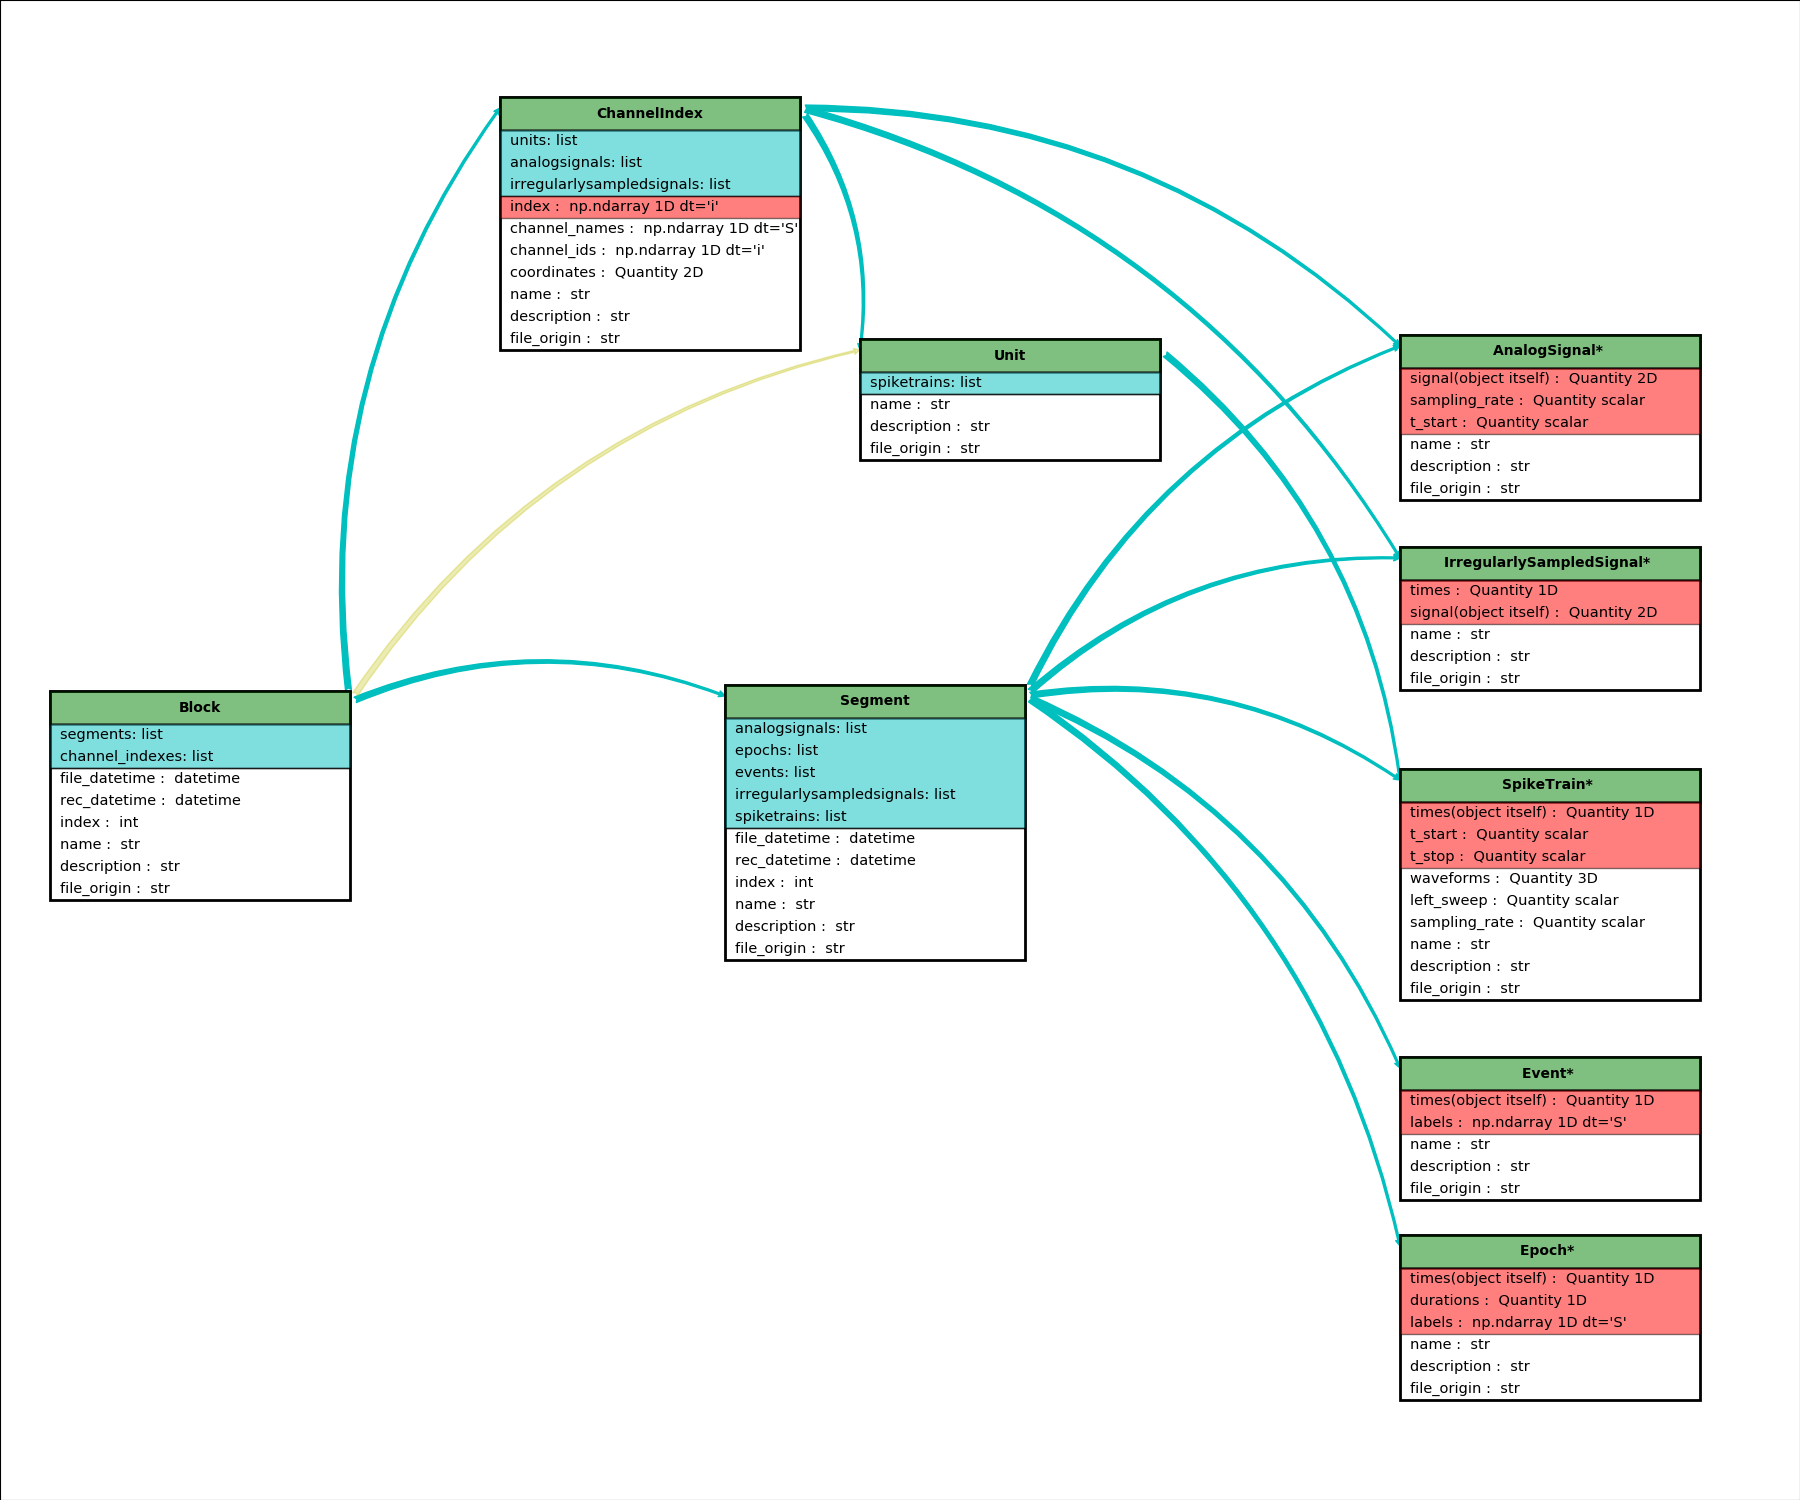
\includegraphics[width=\textwidth]{./Figures/simple_generated_diagram.png}
    \label{fig:neo_uml}
    \caption{Neo 0.7 object structure. Figure modified from \url{https://github.com/neuralensemble/python-neo}.}
\end{figure}


\begin{figure}
    \centering
    \def\svgwidth{\textwidth}
    %LaTeX with PSTricks extensions
%%Creator: inkscape 0.92.4
%%Please note this file requires PSTricks extensions
\psset{xunit=.5pt,yunit=.5pt,runit=.5pt}
\begin{pspicture}(670.67755127,449.88290405)
{
\newrgbcolor{curcolor}{1 1 1}
\pscustom[linestyle=none,fillstyle=solid,fillcolor=curcolor]
{
\newpath
\moveto(0.44696135,449.43594383)
\lineto(670.23059172,449.43594383)
\lineto(670.23059172,0.44696067)
\lineto(0.44696135,0.44696067)
\closepath
}
}
{
\newrgbcolor{curcolor}{1 1 1}
\pscustom[linewidth=0.89392179,linecolor=curcolor]
{
\newpath
\moveto(0.44696135,449.43594383)
\lineto(670.23059172,449.43594383)
\lineto(670.23059172,0.44696067)
\lineto(0.44696135,0.44696067)
\closepath
}
}
{
\newrgbcolor{curcolor}{1 0.80000001 0}
\pscustom[linestyle=none,fillstyle=solid,fillcolor=curcolor]
{
\newpath
\moveto(511.65668634,397.34317869)
\lineto(518.06807018,397.34317869)
\lineto(518.06807018,396.18858626)
\lineto(513.02861381,396.18858626)
\lineto(513.02861381,393.18664595)
\lineto(517.85752685,393.18664595)
\lineto(517.85752685,392.03205352)
\lineto(513.02861381,392.03205352)
\lineto(513.02861381,388.35773291)
\lineto(518.19032114,388.35773291)
\lineto(518.19032114,387.20314048)
\lineto(511.65668634,387.20314048)
\closepath
}
}
{
\newrgbcolor{curcolor}{1 0.80000001 0}
\pscustom[linestyle=none,fillstyle=solid,fillcolor=curcolor]
{
\newpath
\moveto(519.50791518,394.80986707)
\lineto(520.83230061,394.80986707)
\lineto(523.20940267,388.42565011)
\lineto(525.58650473,394.80986707)
\lineto(526.91089016,394.80986707)
\lineto(524.05836769,387.20314048)
\lineto(522.36043765,387.20314048)
\closepath
}
}
{
\newrgbcolor{curcolor}{1 0.80000001 0}
\pscustom[linestyle=none,fillstyle=solid,fillcolor=curcolor]
{
\newpath
\moveto(535.14245468,391.3189229)
\lineto(535.14245468,390.70766809)
\lineto(529.39665942,390.70766809)
\curveto(529.45099318,389.84738354)(529.70907855,389.19085059)(530.17091552,388.73806924)
\curveto(530.63728031,388.28981571)(531.28475763,388.06568894)(532.11334749,388.06568894)
\curveto(532.59329571,388.06568894)(533.05739659,388.12455052)(533.50565012,388.24227367)
\curveto(533.95843147,388.35999682)(534.406685,388.53658154)(534.85041072,388.77202784)
\lineto(534.85041072,387.59026853)
\curveto(534.40215719,387.40010037)(533.94258412,387.25521034)(533.47169152,387.15559844)
\curveto(533.00079892,387.05598655)(532.52311461,387.0061806)(532.03863857,387.0061806)
\curveto(530.82518456,387.0061806)(529.86302421,387.35935005)(529.1521575,388.06568894)
\curveto(528.4458186,388.77202784)(528.09264915,389.72739648)(528.09264915,390.93179485)
\curveto(528.09264915,392.17694355)(528.42770735,393.16400688)(529.09782374,393.89298485)
\curveto(529.77246794,394.62649063)(530.68029453,394.99324351)(531.82130352,394.99324351)
\curveto(532.84458936,394.99324351)(533.65280406,394.66271313)(534.24594762,394.00165237)
\curveto(534.843619,393.34511942)(535.14245468,392.45087627)(535.14245468,391.3189229)
\closepath
\moveto(533.89277817,391.68567579)
\curveto(533.88372255,392.36937562)(533.69129047,392.91497714)(533.31548196,393.32248035)
\curveto(532.94420126,393.72998356)(532.45066959,393.93373517)(531.83488696,393.93373517)
\curveto(531.13760369,393.93373517)(530.57841873,393.73677528)(530.15733208,393.34285551)
\curveto(529.74077324,392.94893574)(529.50079913,392.3942786)(529.43740974,391.67888407)
\closepath
}
}
{
\newrgbcolor{curcolor}{1 0.80000001 0}
\pscustom[linestyle=none,fillstyle=solid,fillcolor=curcolor]
{
\newpath
\moveto(543.51664584,391.79434332)
\lineto(543.51664584,387.20314048)
\lineto(542.26696932,387.20314048)
\lineto(542.26696932,391.753593)
\curveto(542.26696932,392.47351533)(542.12660711,393.01232513)(541.84588267,393.37002239)
\curveto(541.56515824,393.72771966)(541.14407159,393.90656829)(540.58262272,393.90656829)
\curveto(539.90797852,393.90656829)(539.37596044,393.69149715)(538.98656848,393.26135487)
\curveto(538.59717653,392.83121259)(538.40248055,392.24486075)(538.40248055,391.50229935)
\lineto(538.40248055,387.20314048)
\lineto(537.14601232,387.20314048)
\lineto(537.14601232,394.80986707)
\lineto(538.40248055,394.80986707)
\lineto(538.40248055,393.62810776)
\curveto(538.70131624,394.08541692)(539.05222178,394.42726683)(539.45519718,394.65365751)
\curveto(539.86270039,394.88004818)(540.33132908,394.99324351)(540.86108325,394.99324351)
\curveto(541.73495125,394.99324351)(542.39601201,394.72157471)(542.84426554,394.17823709)
\curveto(543.29251907,393.63942729)(543.51664584,392.84479604)(543.51664584,391.79434332)
\closepath
}
}
{
\newrgbcolor{curcolor}{1 0.80000001 0}
\pscustom[linestyle=none,fillstyle=solid,fillcolor=curcolor]
{
\newpath
\moveto(547.25888251,396.96963408)
\lineto(547.25888251,394.80986707)
\lineto(549.83294445,394.80986707)
\lineto(549.83294445,393.83865109)
\lineto(547.25888251,393.83865109)
\lineto(547.25888251,389.70928522)
\curveto(547.25888251,389.08897478)(547.34264706,388.6905272)(547.51017615,388.51394248)
\curveto(547.68223306,388.33735775)(548.02861079,388.24906539)(548.54930934,388.24906539)
\lineto(549.83294445,388.24906539)
\lineto(549.83294445,387.20314048)
\lineto(548.54930934,387.20314048)
\curveto(547.58488508,387.20314048)(546.9192965,387.38198911)(546.55254361,387.73968638)
\curveto(546.18579072,388.10191145)(546.00241428,388.7584444)(546.00241428,389.70928522)
\lineto(546.00241428,393.83865109)
\lineto(545.08553205,393.83865109)
\lineto(545.08553205,394.80986707)
\lineto(546.00241428,394.80986707)
\lineto(546.00241428,396.96963408)
\closepath
}
}
{
\newrgbcolor{curcolor}{0 0 0}
\pscustom[linewidth=1.28582072,linecolor=curcolor]
{
\newpath
\moveto(17.75170226,404.87457298)
\lineto(640.74218077,404.87457298)
\lineto(640.74218077,33.14746116)
\lineto(17.75170226,33.14746116)
\closepath
}
}
{
\newrgbcolor{curcolor}{0.66666669 0.83137256 0}
\pscustom[linewidth=1.16330421,linecolor=curcolor]
{
\newpath
\moveto(249.17607207,155.52130149)
\lineto(377.4213571,155.52130149)
\lineto(377.4213571,144.06550335)
\lineto(249.17607207,144.06550335)
\closepath
}
}
{
\newrgbcolor{curcolor}{1 0.40000001 0}
\pscustom[linewidth=1.16330421,linecolor=curcolor]
{
\newpath
\moveto(240.96714873,223.39184593)
\lineto(630.23991484,223.39184593)
\lineto(630.23991484,210.80626796)
\lineto(240.96714873,210.80626796)
\closepath
}
}
{
\newrgbcolor{curcolor}{0 0 0}
\pscustom[linewidth=1.19684625,linecolor=curcolor]
{
\newpath
\moveto(247.01603789,350.47927879)
\lineto(379.93156523,350.47927879)
\lineto(379.93156523,43.8909304)
\lineto(247.01603789,43.8909304)
\closepath
}
}
{
\newrgbcolor{curcolor}{0 0 0}
\pscustom[linewidth=1.20369136,linecolor=curcolor]
{
\newpath
\moveto(443.79020781,350.48156761)
\lineto(624.54814238,350.48156761)
\lineto(624.54814238,44.16961692)
\lineto(443.79020781,44.16961692)
\closepath
}
}
{
\newrgbcolor{curcolor}{0 0 0.50196081}
\pscustom[linewidth=1.00000004,linecolor=curcolor]
{
\newpath
\moveto(251.31268974,147.02347415)
\lineto(251.31268974,152.60733455)
}
}
{
\newrgbcolor{curcolor}{0 0 0.50196081}
\pscustom[linewidth=1.00000004,linecolor=curcolor]
{
\newpath
\moveto(252.12478744,147.02347415)
\lineto(252.12478744,152.60733455)
}
}
{
\newrgbcolor{curcolor}{0 0 0.50196081}
\pscustom[linewidth=1.00000004,linecolor=curcolor]
{
\newpath
\moveto(254.3807769,147.02347415)
\lineto(254.3807769,152.60733455)
}
}
{
\newrgbcolor{curcolor}{0 0 0.50196081}
\pscustom[linewidth=1.00000004,linecolor=curcolor]
{
\newpath
\moveto(258.70910086,147.02347415)
\lineto(258.70910086,152.60733455)
}
}
{
\newrgbcolor{curcolor}{0 0 0.50196081}
\pscustom[linewidth=1.00000004,linecolor=curcolor]
{
\newpath
\moveto(259.15501049,147.02347415)
\lineto(259.15501049,152.60733455)
}
}
{
\newrgbcolor{curcolor}{0 0 0.50196081}
\pscustom[linewidth=1.00000004,linecolor=curcolor]
{
\newpath
\moveto(260.7565277,147.02347415)
\lineto(260.7565277,152.60733455)
}
}
{
\newrgbcolor{curcolor}{0 0 0.50196081}
\pscustom[linewidth=1.00000004,linecolor=curcolor]
{
\newpath
\moveto(262.82135014,147.02347415)
\lineto(262.82135014,152.60733455)
}
}
{
\newrgbcolor{curcolor}{0 0 0.50196081}
\pscustom[linewidth=1.00000004,linecolor=curcolor]
{
\newpath
\moveto(265.62522295,147.02347415)
\lineto(265.62522295,152.60733455)
}
}
{
\newrgbcolor{curcolor}{0 0 0.50196081}
\pscustom[linewidth=1.00000004,linecolor=curcolor]
{
\newpath
\moveto(268.40258345,147.02347415)
\lineto(268.40258345,152.60733455)
}
}
{
\newrgbcolor{curcolor}{0 0 0.50196081}
\pscustom[linewidth=1.00000004,linecolor=curcolor]
{
\newpath
\moveto(271.68538203,147.02347415)
\lineto(271.68538203,152.60733455)
}
}
{
\newrgbcolor{curcolor}{0 0 0.50196081}
\pscustom[linewidth=1.00000004,linecolor=curcolor]
{
\newpath
\moveto(278.84167704,147.02347415)
\lineto(278.84167704,152.60733455)
}
}
{
\newrgbcolor{curcolor}{0 0 0.50196081}
\pscustom[linewidth=1.00000004,linecolor=curcolor]
{
\newpath
\moveto(280.24604883,147.02347415)
\lineto(280.24604883,152.60733455)
}
}
{
\newrgbcolor{curcolor}{0 0 0.50196081}
\pscustom[linewidth=1.00000004,linecolor=curcolor]
{
\newpath
\moveto(282.42066947,147.02347415)
\lineto(282.42066947,152.60733455)
}
}
{
\newrgbcolor{curcolor}{0 0 0.50196081}
\pscustom[linewidth=1.00000004,linecolor=curcolor]
{
\newpath
\moveto(295.17724065,147.02347415)
\lineto(295.17724065,152.60733455)
}
}
{
\newrgbcolor{curcolor}{0 0 0.50196081}
\pscustom[linewidth=1.00000004,linecolor=curcolor]
{
\newpath
\moveto(296.37204159,147.02347415)
\lineto(296.37204159,152.60733455)
}
}
{
\newrgbcolor{curcolor}{0 0 0.50196081}
\pscustom[linewidth=1.00000004,linecolor=curcolor]
{
\newpath
\moveto(300.52684974,147.02347415)
\lineto(300.52684974,152.60733455)
}
}
{
\newrgbcolor{curcolor}{0 0 0.50196081}
\pscustom[linewidth=1.00000004,linecolor=curcolor]
{
\newpath
\moveto(300.92003294,147.02347415)
\lineto(300.92003294,152.60733455)
}
}
{
\newrgbcolor{curcolor}{0 0 0.50196081}
\pscustom[linewidth=1.00000004,linecolor=curcolor]
{
\newpath
\moveto(303.48674335,147.02347415)
\lineto(303.48674335,152.60733455)
}
}
{
\newrgbcolor{curcolor}{0 0 0.50196081}
\pscustom[linewidth=1.00000004,linecolor=curcolor]
{
\newpath
\moveto(306.62796304,147.02347415)
\lineto(306.62796304,152.60733455)
}
}
{
\newrgbcolor{curcolor}{0 0 0.50196081}
\pscustom[linewidth=1.00000004,linecolor=curcolor]
{
\newpath
\moveto(308.38439341,147.02347415)
\lineto(308.38439341,152.60733455)
}
}
{
\newrgbcolor{curcolor}{0 0 0.50196081}
\pscustom[linewidth=1.00000004,linecolor=curcolor]
{
\newpath
\moveto(310.89779517,147.02347415)
\lineto(310.89779517,152.60733455)
}
}
{
\newrgbcolor{curcolor}{0 0 0.50196081}
\pscustom[linewidth=1.00000004,linecolor=curcolor]
{
\newpath
\moveto(314.57249892,147.02347415)
\lineto(314.57249892,152.60733455)
}
}
{
\newrgbcolor{curcolor}{0 0 0.50196081}
\pscustom[linewidth=1.00000004,linecolor=curcolor]
{
\newpath
\moveto(314.62772463,147.02347415)
\lineto(314.62772463,152.60733455)
}
}
{
\newrgbcolor{curcolor}{0 0 0.50196081}
\pscustom[linewidth=1.00000004,linecolor=curcolor]
{
\newpath
\moveto(315.83976496,147.02347415)
\lineto(315.83976496,152.60733455)
}
}
{
\newrgbcolor{curcolor}{0 0 0.50196081}
\pscustom[linewidth=1.00000004,linecolor=curcolor]
{
\newpath
\moveto(317.14471911,147.02347415)
\lineto(317.14471911,152.60733455)
}
}
{
\newrgbcolor{curcolor}{0 0 0.50196081}
\pscustom[linewidth=1.00000004,linecolor=curcolor]
{
\newpath
\moveto(318.93540107,147.02347415)
\lineto(318.93540107,152.60733455)
}
}
{
\newrgbcolor{curcolor}{0 0 0.50196081}
\pscustom[linewidth=1.00000004,linecolor=curcolor]
{
\newpath
\moveto(322.22909143,147.02347415)
\lineto(322.22909143,152.60733455)
}
}
{
\newrgbcolor{curcolor}{0 0 0.50196081}
\pscustom[linewidth=1.00000004,linecolor=curcolor]
{
\newpath
\moveto(323.41413663,147.02347415)
\lineto(323.41413663,152.60733455)
}
}
{
\newrgbcolor{curcolor}{0 0 0.50196081}
\pscustom[linewidth=1.00000004,linecolor=curcolor]
{
\newpath
\moveto(325.41561068,147.02347415)
\lineto(325.41561068,152.60733455)
}
}
{
\newrgbcolor{curcolor}{0 0 0.50196081}
\pscustom[linewidth=1.00000004,linecolor=curcolor]
{
\newpath
\moveto(327.26423065,147.02347415)
\lineto(327.26423065,152.60733455)
}
}
{
\newrgbcolor{curcolor}{0 0 0.50196081}
\pscustom[linewidth=1.00000004,linecolor=curcolor]
{
\newpath
\moveto(334.70341364,147.02347415)
\lineto(334.70341364,152.60733455)
}
}
{
\newrgbcolor{curcolor}{0 0 0.50196081}
\pscustom[linewidth=1.00000004,linecolor=curcolor]
{
\newpath
\moveto(336.38946638,147.02347415)
\lineto(336.38946638,152.60733455)
}
}
{
\newrgbcolor{curcolor}{0 0 0.50196081}
\pscustom[linewidth=1.00000004,linecolor=curcolor]
{
\newpath
\moveto(337.25988549,147.02347415)
\lineto(337.25988549,152.60733455)
}
}
{
\newrgbcolor{curcolor}{0 0 0.50196081}
\pscustom[linewidth=1.00000004,linecolor=curcolor]
{
\newpath
\moveto(339.69154923,147.02347415)
\lineto(339.69154923,152.60733455)
}
}
{
\newrgbcolor{curcolor}{0 0 0.50196081}
\pscustom[linewidth=1.00000004,linecolor=curcolor]
{
\newpath
\moveto(342.97186273,147.02347415)
\lineto(342.97186273,152.60733455)
}
}
{
\newrgbcolor{curcolor}{0 0 0.50196081}
\pscustom[linewidth=1.00000004,linecolor=curcolor]
{
\newpath
\moveto(343.64678368,147.02347415)
\lineto(343.64678368,152.60733455)
}
}
{
\newrgbcolor{curcolor}{0 0 0.50196081}
\pscustom[linewidth=1.00000004,linecolor=curcolor]
{
\newpath
\moveto(344.48682794,147.02347415)
\lineto(344.48682794,152.60733455)
}
}
{
\newrgbcolor{curcolor}{0 0 0.50196081}
\pscustom[linewidth=1.00000004,linecolor=curcolor]
{
\newpath
\moveto(345.53400058,147.02347415)
\lineto(345.53400058,152.60733455)
}
}
{
\newrgbcolor{curcolor}{0 0 0.50196081}
\pscustom[linewidth=1.00000004,linecolor=curcolor]
{
\newpath
\moveto(346.09994696,147.02347415)
\lineto(346.09994696,152.60733455)
}
}
{
\newrgbcolor{curcolor}{0 0 0.50196081}
\pscustom[linewidth=1.00000004,linecolor=curcolor]
{
\newpath
\moveto(353.01692108,147.02347415)
\lineto(353.01692108,152.60733455)
}
}
{
\newrgbcolor{curcolor}{0 0 0.50196081}
\pscustom[linewidth=1.00000004,linecolor=curcolor]
{
\newpath
\moveto(353.14884365,147.02347415)
\lineto(353.14884365,152.60733455)
}
}
{
\newrgbcolor{curcolor}{0 0 0.50196081}
\pscustom[linewidth=1.00000004,linecolor=curcolor]
{
\newpath
\moveto(363.00614311,147.02347415)
\lineto(363.00614311,152.60733455)
}
}
{
\newrgbcolor{curcolor}{0 0 0.50196081}
\pscustom[linewidth=1.00000004,linecolor=curcolor]
{
\newpath
\moveto(363.4914307,147.02347415)
\lineto(363.4914307,152.60733455)
}
}
{
\newrgbcolor{curcolor}{0 0 0.50196081}
\pscustom[linewidth=1.00000004,linecolor=curcolor]
{
\newpath
\moveto(366.2084391,147.02347415)
\lineto(366.2084391,152.60733455)
}
}
{
\newrgbcolor{curcolor}{0 0 0.50196081}
\pscustom[linewidth=1.00000004,linecolor=curcolor]
{
\newpath
\moveto(371.16588743,147.02347415)
\lineto(371.16588743,152.60733455)
}
}
{
\newrgbcolor{curcolor}{0 0 0.50196081}
\pscustom[linewidth=1.00000004,linecolor=curcolor]
{
\newpath
\moveto(374.066707,147.02347415)
\lineto(374.066707,152.60733455)
}
}
{
\newrgbcolor{curcolor}{0 0 0.50196081}
\pscustom[linewidth=1.00000004,linecolor=curcolor]
{
\newpath
\moveto(375.52177454,147.02347415)
\lineto(375.52177454,152.60733455)
}
}
{
\newrgbcolor{curcolor}{0 0 0.50196081}
\pscustom[linewidth=1.00000004,linecolor=curcolor]
{
\newpath
\moveto(449.86589083,147.02347415)
\lineto(449.86589083,152.60733455)
}
}
{
\newrgbcolor{curcolor}{0 0 0.50196081}
\pscustom[linewidth=1.00000004,linecolor=curcolor]
{
\newpath
\moveto(452.45412918,147.02347415)
\lineto(452.45412918,152.60733455)
}
}
{
\newrgbcolor{curcolor}{0 0 0.50196081}
\pscustom[linewidth=1.00000004,linecolor=curcolor]
{
\newpath
\moveto(456.43128919,147.02347415)
\lineto(456.43128919,152.60733455)
}
}
{
\newrgbcolor{curcolor}{0 0 0.50196081}
\pscustom[linewidth=1.00000004,linecolor=curcolor]
{
\newpath
\moveto(458.88635533,147.02347415)
\lineto(458.88635533,152.60733455)
}
}
{
\newrgbcolor{curcolor}{0 0 0.50196081}
\pscustom[linewidth=1.00000004,linecolor=curcolor]
{
\newpath
\moveto(460.14625133,147.02347415)
\lineto(460.14625133,152.60733455)
}
}
{
\newrgbcolor{curcolor}{0 0 0.50196081}
\pscustom[linewidth=1.00000004,linecolor=curcolor]
{
\newpath
\moveto(463.42903571,147.02347415)
\lineto(463.42903571,152.60733455)
}
}
{
\newrgbcolor{curcolor}{0 0 0.50196081}
\pscustom[linewidth=1.00000004,linecolor=curcolor]
{
\newpath
\moveto(467.39617017,147.02347415)
\lineto(467.39617017,152.60733455)
}
}
{
\newrgbcolor{curcolor}{0 0 0.50196081}
\pscustom[linewidth=1.00000004,linecolor=curcolor]
{
\newpath
\moveto(468.85322579,147.02347415)
\lineto(468.85322579,152.60733455)
}
}
{
\newrgbcolor{curcolor}{0 0 0.50196081}
\pscustom[linewidth=1.00000004,linecolor=curcolor]
{
\newpath
\moveto(471.80908646,147.02347415)
\lineto(471.80908646,152.60733455)
}
}
{
\newrgbcolor{curcolor}{0 0 0.50196081}
\pscustom[linewidth=1.00000004,linecolor=curcolor]
{
\newpath
\moveto(472.81439604,147.02347415)
\lineto(472.81439604,152.60733455)
}
}
{
\newrgbcolor{curcolor}{0 0 0.50196081}
\pscustom[linewidth=1.00000004,linecolor=curcolor]
{
\newpath
\moveto(475.59292098,147.02347415)
\lineto(475.59292098,152.60733455)
}
}
{
\newrgbcolor{curcolor}{0 0 0.50196081}
\pscustom[linewidth=1.00000004,linecolor=curcolor]
{
\newpath
\moveto(476.88468287,147.02347415)
\lineto(476.88468287,152.60733455)
}
}
{
\newrgbcolor{curcolor}{0 0 0.50196081}
\pscustom[linewidth=1.00000004,linecolor=curcolor]
{
\newpath
\moveto(478.93534742,147.02347415)
\lineto(478.93534742,152.60733455)
}
}
{
\newrgbcolor{curcolor}{0 0 0.50196081}
\pscustom[linewidth=1.00000004,linecolor=curcolor]
{
\newpath
\moveto(482.13378089,147.02347415)
\lineto(482.13378089,152.60733455)
}
}
{
\newrgbcolor{curcolor}{0 0 0.50196081}
\pscustom[linewidth=1.00000004,linecolor=curcolor]
{
\newpath
\moveto(492.96966461,147.02347415)
\lineto(492.96966461,152.60733455)
}
}
{
\newrgbcolor{curcolor}{0 0 0.50196081}
\pscustom[linewidth=1.00000004,linecolor=curcolor]
{
\newpath
\moveto(493.8047387,147.02347415)
\lineto(493.8047387,152.60733455)
}
}
{
\newrgbcolor{curcolor}{0 0 0.50196081}
\pscustom[linewidth=1.00000004,linecolor=curcolor]
{
\newpath
\moveto(495.91035915,147.02347415)
\lineto(495.91035915,152.60733455)
}
}
{
\newrgbcolor{curcolor}{0 0 0.50196081}
\pscustom[linewidth=1.00000004,linecolor=curcolor]
{
\newpath
\moveto(497.27460036,147.02347415)
\lineto(497.27460036,152.60733455)
}
}
{
\newrgbcolor{curcolor}{0 0 0.50196081}
\pscustom[linewidth=1.00000004,linecolor=curcolor]
{
\newpath
\moveto(502.44494245,147.02347415)
\lineto(502.44494245,152.60733455)
}
}
{
\newrgbcolor{curcolor}{0 0 0.50196081}
\pscustom[linewidth=1.00000004,linecolor=curcolor]
{
\newpath
\moveto(504.19898714,147.02347415)
\lineto(504.19898714,152.60733455)
}
}
{
\newrgbcolor{curcolor}{0 0 0.50196081}
\pscustom[linewidth=1.00000004,linecolor=curcolor]
{
\newpath
\moveto(512.06640015,147.02347415)
\lineto(512.06640015,152.60733455)
}
}
{
\newrgbcolor{curcolor}{0 0 0.50196081}
\pscustom[linewidth=1.00000004,linecolor=curcolor]
{
\newpath
\moveto(515.34625923,147.02347415)
\lineto(515.34625923,152.60733455)
}
}
{
\newrgbcolor{curcolor}{0 0 0.50196081}
\pscustom[linewidth=1.00000004,linecolor=curcolor]
{
\newpath
\moveto(516.80754659,147.02347415)
\lineto(516.80754659,152.60733455)
}
}
{
\newrgbcolor{curcolor}{0 0 0.50196081}
\pscustom[linewidth=1.00000004,linecolor=curcolor]
{
\newpath
\moveto(519.92716733,147.02347415)
\lineto(519.92716733,152.60733455)
}
}
{
\newrgbcolor{curcolor}{0 0 0.50196081}
\pscustom[linewidth=1.00000004,linecolor=curcolor]
{
\newpath
\moveto(532.41581783,147.02347415)
\lineto(532.41581783,152.60733455)
}
}
{
\newrgbcolor{curcolor}{0 0 0.50196081}
\pscustom[linewidth=1.00000004,linecolor=curcolor]
{
\newpath
\moveto(545.96001926,147.02347415)
\lineto(545.96001926,152.60733455)
}
}
{
\newrgbcolor{curcolor}{0 0 0.50196081}
\pscustom[linewidth=1.00000004,linecolor=curcolor]
{
\newpath
\moveto(546.32599432,147.02347415)
\lineto(546.32599432,152.60733455)
}
}
{
\newrgbcolor{curcolor}{0 0 0.50196081}
\pscustom[linewidth=1.00000004,linecolor=curcolor]
{
\newpath
\moveto(549.14198015,147.02347415)
\lineto(549.14198015,152.60733455)
}
}
{
\newrgbcolor{curcolor}{0 0 0.50196081}
\pscustom[linewidth=1.00000004,linecolor=curcolor]
{
\newpath
\moveto(551.17850102,147.02347415)
\lineto(551.17850102,152.60733455)
}
}
{
\newrgbcolor{curcolor}{0 0 0.50196081}
\pscustom[linewidth=1.00000004,linecolor=curcolor]
{
\newpath
\moveto(551.32740737,147.02347415)
\lineto(551.32740737,152.60733455)
}
}
{
\newrgbcolor{curcolor}{0 0 0.50196081}
\pscustom[linewidth=1.00000004,linecolor=curcolor]
{
\newpath
\moveto(552.68173663,147.02347415)
\lineto(552.68173663,152.60733455)
}
}
{
\newrgbcolor{curcolor}{0 0 0.50196081}
\pscustom[linewidth=1.00000004,linecolor=curcolor]
{
\newpath
\moveto(554.52010384,147.02347415)
\lineto(554.52010384,152.60733455)
}
}
{
\newrgbcolor{curcolor}{0 0 0.50196081}
\pscustom[linewidth=1.00000004,linecolor=curcolor]
{
\newpath
\moveto(555.63336555,147.02347415)
\lineto(555.63336555,152.60733455)
}
}
{
\newrgbcolor{curcolor}{0 0 0.50196081}
\pscustom[linewidth=1.00000004,linecolor=curcolor]
{
\newpath
\moveto(562.41455458,147.02347415)
\lineto(562.41455458,152.60733455)
}
}
{
\newrgbcolor{curcolor}{0 0 0.50196081}
\pscustom[linewidth=1.00000004,linecolor=curcolor]
{
\newpath
\moveto(564.83656198,147.02347415)
\lineto(564.83656198,152.60733455)
}
}
{
\newrgbcolor{curcolor}{0 0 0.50196081}
\pscustom[linewidth=1.00000004,linecolor=curcolor]
{
\newpath
\moveto(565.06922283,147.02347415)
\lineto(565.06922283,152.60733455)
}
}
{
\newrgbcolor{curcolor}{0 0 0.50196081}
\pscustom[linewidth=1.00000004,linecolor=curcolor]
{
\newpath
\moveto(573.21777717,147.02347415)
\lineto(573.21777717,152.60733455)
}
}
{
\newrgbcolor{curcolor}{0 0 0.50196081}
\pscustom[linewidth=1.00000004,linecolor=curcolor]
{
\newpath
\moveto(578.65349804,147.02347415)
\lineto(578.65349804,152.60733455)
}
}
{
\newrgbcolor{curcolor}{0 0 0.50196081}
\pscustom[linewidth=1.00000004,linecolor=curcolor]
{
\newpath
\moveto(579.7215738,147.02347415)
\lineto(579.7215738,152.60733455)
}
}
{
\newrgbcolor{curcolor}{0 0 0.50196081}
\pscustom[linewidth=1.00000004,linecolor=curcolor]
{
\newpath
\moveto(586.89304913,147.02347415)
\lineto(586.89304913,152.60733455)
}
}
{
\newrgbcolor{curcolor}{0 0 0.50196081}
\pscustom[linewidth=1.00000004,linecolor=curcolor]
{
\newpath
\moveto(587.63175869,147.02347415)
\lineto(587.63175869,152.60733455)
}
}
{
\newrgbcolor{curcolor}{0 0 0.50196081}
\pscustom[linewidth=1.00000004,linecolor=curcolor]
{
\newpath
\moveto(588.78137367,147.02347415)
\lineto(588.78137367,152.60733455)
}
}
{
\newrgbcolor{curcolor}{0 0 0.50196081}
\pscustom[linewidth=1.00000004,linecolor=curcolor]
{
\newpath
\moveto(592.55018407,147.02347415)
\lineto(592.55018407,152.60733455)
}
}
{
\newrgbcolor{curcolor}{0 0 0.50196081}
\pscustom[linewidth=1.00000004,linecolor=curcolor]
{
\newpath
\moveto(594.44231433,147.02347415)
\lineto(594.44231433,152.60733455)
}
}
{
\newrgbcolor{curcolor}{0 0 0.50196081}
\pscustom[linewidth=1.00000004,linecolor=curcolor]
{
\newpath
\moveto(594.60567678,147.02347415)
\lineto(594.60567678,152.60733455)
}
}
{
\newrgbcolor{curcolor}{0 0 0.50196081}
\pscustom[linewidth=1.00000004,linecolor=curcolor]
{
\newpath
\moveto(605.89353374,147.02347415)
\lineto(605.89353374,152.60733455)
}
}
{
\newrgbcolor{curcolor}{0 0 0.50196081}
\pscustom[linewidth=1.00000004,linecolor=curcolor]
{
\newpath
\moveto(610.84081452,147.02347415)
\lineto(610.84081452,152.60733455)
}
}
{
\newrgbcolor{curcolor}{0 0 0.50196081}
\pscustom[linewidth=1.00000004,linecolor=curcolor]
{
\newpath
\moveto(614.71056201,147.02347415)
\lineto(614.71056201,152.60733455)
}
}
{
\newrgbcolor{curcolor}{0 0 0.50196081}
\pscustom[linewidth=1.00000004,linecolor=curcolor]
{
\newpath
\moveto(621.6209187,147.02347415)
\lineto(621.6209187,152.60733455)
}
}
{
\newrgbcolor{curcolor}{0 0 0.50196081}
\pscustom[linewidth=1.00000004,linecolor=curcolor]
{
\newpath
\moveto(623.82455095,147.02347415)
\lineto(623.82455095,152.60733455)
}
}
{
\newrgbcolor{curcolor}{0.21568628 0.27058825 0.28235295}
\pscustom[linewidth=1.00000005,linecolor=curcolor]
{
\newpath
\moveto(248.70713287,214.49752495)
\lineto(248.70713287,220.15642855)
}
}
{
\newrgbcolor{curcolor}{0.21568628 0.27058825 0.28235295}
\pscustom[linewidth=1.00000005,linecolor=curcolor]
{
\newpath
\moveto(249.36093237,214.49752495)
\lineto(249.36093237,220.15642855)
}
}
{
\newrgbcolor{curcolor}{0.21568628 0.27058825 0.28235295}
\pscustom[linewidth=1.00000005,linecolor=curcolor]
{
\newpath
\moveto(250.35543151,214.49752495)
\lineto(250.35543151,220.15642855)
}
}
{
\newrgbcolor{curcolor}{0.21568628 0.27058825 0.28235295}
\pscustom[linewidth=1.00000005,linecolor=curcolor]
{
\newpath
\moveto(252.35562741,214.49752495)
\lineto(252.35562741,220.15642855)
}
}
{
\newrgbcolor{curcolor}{0.21568628 0.27058825 0.28235295}
\pscustom[linewidth=1.00000005,linecolor=curcolor]
{
\newpath
\moveto(252.56562235,214.49752495)
\lineto(252.56562235,220.15642855)
}
}
{
\newrgbcolor{curcolor}{0.21568628 0.27058825 0.28235295}
\pscustom[linewidth=1.00000005,linecolor=curcolor]
{
\newpath
\moveto(253.03604099,214.49752495)
\lineto(253.03604099,220.15642855)
}
}
{
\newrgbcolor{curcolor}{0.21568628 0.27058825 0.28235295}
\pscustom[linewidth=1.00000005,linecolor=curcolor]
{
\newpath
\moveto(256.63666961,214.49752495)
\lineto(256.63666961,220.15642855)
}
}
{
\newrgbcolor{curcolor}{0.21568628 0.27058825 0.28235295}
\pscustom[linewidth=1.00000005,linecolor=curcolor]
{
\newpath
\moveto(258.94452427,214.49752495)
\lineto(258.94452427,220.15642855)
}
}
{
\newrgbcolor{curcolor}{0.21568628 0.27058825 0.28235295}
\pscustom[linewidth=1.00000005,linecolor=curcolor]
{
\newpath
\moveto(259.71956568,214.49752495)
\lineto(259.71956568,220.15642855)
}
}
{
\newrgbcolor{curcolor}{0.21568628 0.27058825 0.28235295}
\pscustom[linewidth=1.00000005,linecolor=curcolor]
{
\newpath
\moveto(262.57779949,214.49752495)
\lineto(262.57779949,220.15642855)
}
}
{
\newrgbcolor{curcolor}{0.21568628 0.27058825 0.28235295}
\pscustom[linewidth=1.00000005,linecolor=curcolor]
{
\newpath
\moveto(262.98836602,214.49752495)
\lineto(262.98836602,220.15642855)
}
}
{
\newrgbcolor{curcolor}{0.21568628 0.27058825 0.28235295}
\pscustom[linewidth=1.00000005,linecolor=curcolor]
{
\newpath
\moveto(268.00655907,214.49752495)
\lineto(268.00655907,220.15642855)
}
}
{
\newrgbcolor{curcolor}{0.21568628 0.27058825 0.28235295}
\pscustom[linewidth=1.00000005,linecolor=curcolor]
{
\newpath
\moveto(275.77865874,214.49752495)
\lineto(275.77865874,220.15642855)
}
}
{
\newrgbcolor{curcolor}{0.21568628 0.27058825 0.28235295}
\pscustom[linewidth=1.00000005,linecolor=curcolor]
{
\newpath
\moveto(276.10603163,214.49752495)
\lineto(276.10603163,220.15642855)
}
}
{
\newrgbcolor{curcolor}{0.21568628 0.27058825 0.28235295}
\pscustom[linewidth=1.00000005,linecolor=curcolor]
{
\newpath
\moveto(278.06644441,214.49752495)
\lineto(278.06644441,220.15642855)
}
}
{
\newrgbcolor{curcolor}{0.21568628 0.27058825 0.28235295}
\pscustom[linewidth=1.00000005,linecolor=curcolor]
{
\newpath
\moveto(278.20700618,214.49752495)
\lineto(278.20700618,220.15642855)
}
}
{
\newrgbcolor{curcolor}{0.21568628 0.27058825 0.28235295}
\pscustom[linewidth=1.00000005,linecolor=curcolor]
{
\newpath
\moveto(279.68280615,214.49752495)
\lineto(279.68280615,220.15642855)
}
}
{
\newrgbcolor{curcolor}{0.21568628 0.27058825 0.28235295}
\pscustom[linewidth=1.00000005,linecolor=curcolor]
{
\newpath
\moveto(280.6554226,214.49752495)
\lineto(280.6554226,220.15642855)
}
}
{
\newrgbcolor{curcolor}{0.21568628 0.27058825 0.28235295}
\pscustom[linewidth=1.00000005,linecolor=curcolor]
{
\newpath
\moveto(281.59901985,214.49752495)
\lineto(281.59901985,220.15642855)
}
}
{
\newrgbcolor{curcolor}{0.21568628 0.27058825 0.28235295}
\pscustom[linewidth=1.00000005,linecolor=curcolor]
{
\newpath
\moveto(283.29277927,214.49752495)
\lineto(283.29277927,220.15642855)
}
}
{
\newrgbcolor{curcolor}{0.21568628 0.27058825 0.28235295}
\pscustom[linewidth=1.00000005,linecolor=curcolor]
{
\newpath
\moveto(284.34874708,214.49752495)
\lineto(284.34874708,220.15642855)
}
}
{
\newrgbcolor{curcolor}{0.21568628 0.27058825 0.28235295}
\pscustom[linewidth=1.00000005,linecolor=curcolor]
{
\newpath
\moveto(285.72972207,214.49752495)
\lineto(285.72972207,220.15642855)
}
}
{
\newrgbcolor{curcolor}{0.21568628 0.27058825 0.28235295}
\pscustom[linewidth=1.00000005,linecolor=curcolor]
{
\newpath
\moveto(285.94365984,214.49752495)
\lineto(285.94365984,220.15642855)
}
}
{
\newrgbcolor{curcolor}{0.21568628 0.27058825 0.28235295}
\pscustom[linewidth=1.00000005,linecolor=curcolor]
{
\newpath
\moveto(287.31446234,214.49752495)
\lineto(287.31446234,220.15642855)
}
}
{
\newrgbcolor{curcolor}{0.21568628 0.27058825 0.28235295}
\pscustom[linewidth=1.00000005,linecolor=curcolor]
{
\newpath
\moveto(295.90272711,214.49752495)
\lineto(295.90272711,220.15642855)
}
}
{
\newrgbcolor{curcolor}{0.21568628 0.27058825 0.28235295}
\pscustom[linewidth=1.00000005,linecolor=curcolor]
{
\newpath
\moveto(301.02891417,214.49752495)
\lineto(301.02891417,220.15642855)
}
}
{
\newrgbcolor{curcolor}{0.21568628 0.27058825 0.28235295}
\pscustom[linewidth=1.00000005,linecolor=curcolor]
{
\newpath
\moveto(301.37860346,214.49752495)
\lineto(301.37860346,220.15642855)
}
}
{
\newrgbcolor{curcolor}{0.21568628 0.27058825 0.28235295}
\pscustom[linewidth=1.00000005,linecolor=curcolor]
{
\newpath
\moveto(309.31886468,214.49752495)
\lineto(309.31886468,220.15642855)
}
}
{
\newrgbcolor{curcolor}{0.21568628 0.27058825 0.28235295}
\pscustom[linewidth=1.00000005,linecolor=curcolor]
{
\newpath
\moveto(309.4956216,214.49752495)
\lineto(309.4956216,220.15642855)
}
}
{
\newrgbcolor{curcolor}{0.21568628 0.27058825 0.28235295}
\pscustom[linewidth=1.00000005,linecolor=curcolor]
{
\newpath
\moveto(312.71020807,214.49752495)
\lineto(312.71020807,220.15642855)
}
}
{
\newrgbcolor{curcolor}{0.21568628 0.27058825 0.28235295}
\pscustom[linewidth=1.00000005,linecolor=curcolor]
{
\newpath
\moveto(323.20179349,214.49752495)
\lineto(323.20179349,220.15642855)
}
}
{
\newrgbcolor{curcolor}{0.21568628 0.27058825 0.28235295}
\pscustom[linewidth=1.00000005,linecolor=curcolor]
{
\newpath
\moveto(335.28781854,214.49752495)
\lineto(335.28781854,220.15642855)
}
}
{
\newrgbcolor{curcolor}{0.21568628 0.27058825 0.28235295}
\pscustom[linewidth=1.00000005,linecolor=curcolor]
{
\newpath
\moveto(336.01925229,214.49752495)
\lineto(336.01925229,220.15642855)
}
}
{
\newrgbcolor{curcolor}{0.21568628 0.27058825 0.28235295}
\pscustom[linewidth=1.00000005,linecolor=curcolor]
{
\newpath
\moveto(338.6637849,214.49752495)
\lineto(338.6637849,220.15642855)
}
}
{
\newrgbcolor{curcolor}{0.21568628 0.27058825 0.28235295}
\pscustom[linewidth=1.00000005,linecolor=curcolor]
{
\newpath
\moveto(340.08162533,214.49752495)
\lineto(340.08162533,220.15642855)
}
}
{
\newrgbcolor{curcolor}{0.21568628 0.27058825 0.28235295}
\pscustom[linewidth=1.00000005,linecolor=curcolor]
{
\newpath
\moveto(344.23961191,214.49752495)
\lineto(344.23961191,220.15642855)
}
}
{
\newrgbcolor{curcolor}{0.21568628 0.27058825 0.28235295}
\pscustom[linewidth=1.00000005,linecolor=curcolor]
{
\newpath
\moveto(344.3167336,214.49752495)
\lineto(344.3167336,220.15642855)
}
}
{
\newrgbcolor{curcolor}{0.21568628 0.27058825 0.28235295}
\pscustom[linewidth=1.00000005,linecolor=curcolor]
{
\newpath
\moveto(348.12775144,214.49752495)
\lineto(348.12775144,220.15642855)
}
}
{
\newrgbcolor{curcolor}{0.21568628 0.27058825 0.28235295}
\pscustom[linewidth=1.00000005,linecolor=curcolor]
{
\newpath
\moveto(349.00436007,214.49752495)
\lineto(349.00436007,220.15642855)
}
}
{
\newrgbcolor{curcolor}{0.21568628 0.27058825 0.28235295}
\pscustom[linewidth=1.00000005,linecolor=curcolor]
{
\newpath
\moveto(349.34446828,214.49752495)
\lineto(349.34446828,220.15642855)
}
}
{
\newrgbcolor{curcolor}{0.21568628 0.27058825 0.28235295}
\pscustom[linewidth=1.00000005,linecolor=curcolor]
{
\newpath
\moveto(350.86174679,214.49752495)
\lineto(350.86174679,220.15642855)
}
}
{
\newrgbcolor{curcolor}{0.21568628 0.27058825 0.28235295}
\pscustom[linewidth=1.00000005,linecolor=curcolor]
{
\newpath
\moveto(355.15718031,214.49752495)
\lineto(355.15718031,220.15642855)
}
}
{
\newrgbcolor{curcolor}{0.21568628 0.27058825 0.28235295}
\pscustom[linewidth=1.00000005,linecolor=curcolor]
{
\newpath
\moveto(357.51021976,214.49752495)
\lineto(357.51021976,220.15642855)
}
}
{
\newrgbcolor{curcolor}{0.21568628 0.27058825 0.28235295}
\pscustom[linewidth=1.00000005,linecolor=curcolor]
{
\newpath
\moveto(359.69170683,214.49752495)
\lineto(359.69170683,220.15642855)
}
}
{
\newrgbcolor{curcolor}{0.21568628 0.27058825 0.28235295}
\pscustom[linewidth=1.00000005,linecolor=curcolor]
{
\newpath
\moveto(360.73462387,214.49752495)
\lineto(360.73462387,220.15642855)
}
}
{
\newrgbcolor{curcolor}{0.21568628 0.27058825 0.28235295}
\pscustom[linewidth=1.00000005,linecolor=curcolor]
{
\newpath
\moveto(363.31027531,214.49752495)
\lineto(363.31027531,220.15642855)
}
}
{
\newrgbcolor{curcolor}{0.21568628 0.27058825 0.28235295}
\pscustom[linewidth=1.00000005,linecolor=curcolor]
{
\newpath
\moveto(365.94100803,214.49752495)
\lineto(365.94100803,220.15642855)
}
}
{
\newrgbcolor{curcolor}{0.21568628 0.27058825 0.28235295}
\pscustom[linewidth=1.00000005,linecolor=curcolor]
{
\newpath
\moveto(368.86193279,214.49752495)
\lineto(368.86193279,220.15642855)
}
}
{
\newrgbcolor{curcolor}{0.21568628 0.27058825 0.28235295}
\pscustom[linewidth=1.00000005,linecolor=curcolor]
{
\newpath
\moveto(369.51738827,214.49752495)
\lineto(369.51738827,220.15642855)
}
}
{
\newrgbcolor{curcolor}{0.21568628 0.27058825 0.28235295}
\pscustom[linewidth=1.00000005,linecolor=curcolor]
{
\newpath
\moveto(372.89966316,214.49752495)
\lineto(372.89966316,220.15642855)
}
}
{
\newrgbcolor{curcolor}{0.21568628 0.27058825 0.28235295}
\pscustom[linewidth=1.00000005,linecolor=curcolor]
{
\newpath
\moveto(373.05043685,214.49752495)
\lineto(373.05043685,220.15642855)
}
}
{
\newrgbcolor{curcolor}{0.21568628 0.27058825 0.28235295}
\pscustom[linewidth=1.00000005,linecolor=curcolor]
{
\newpath
\moveto(373.84933236,214.49752495)
\lineto(373.84933236,220.15642855)
}
}
{
\newrgbcolor{curcolor}{0.21568628 0.27058825 0.28235295}
\pscustom[linewidth=1.00000005,linecolor=curcolor]
{
\newpath
\moveto(374.7696275,214.49752495)
\lineto(374.7696275,220.15642855)
}
}
{
\newrgbcolor{curcolor}{0.21568628 0.27058825 0.28235295}
\pscustom[linewidth=1.00000005,linecolor=curcolor]
{
\newpath
\moveto(448.72880255,214.49752495)
\lineto(448.72880255,220.15642855)
}
}
{
\newrgbcolor{curcolor}{0.21568628 0.27058825 0.28235295}
\pscustom[linewidth=1.00000005,linecolor=curcolor]
{
\newpath
\moveto(450.91474501,214.49752495)
\lineto(450.91474501,220.15642855)
}
}
{
\newrgbcolor{curcolor}{0.21568628 0.27058825 0.28235295}
\pscustom[linewidth=1.00000005,linecolor=curcolor]
{
\newpath
\moveto(458.01226649,214.49752495)
\lineto(458.01226649,220.15642855)
}
}
{
\newrgbcolor{curcolor}{0.21568628 0.27058825 0.28235295}
\pscustom[linewidth=1.00000005,linecolor=curcolor]
{
\newpath
\moveto(460.36818421,214.49752495)
\lineto(460.36818421,220.15642855)
}
}
{
\newrgbcolor{curcolor}{0.21568628 0.27058825 0.28235295}
\pscustom[linewidth=1.00000005,linecolor=curcolor]
{
\newpath
\moveto(461.44595584,214.49752495)
\lineto(461.44595584,220.15642855)
}
}
{
\newrgbcolor{curcolor}{0.21568628 0.27058825 0.28235295}
\pscustom[linewidth=1.00000005,linecolor=curcolor]
{
\newpath
\moveto(461.86026805,214.49752495)
\lineto(461.86026805,220.15642855)
}
}
{
\newrgbcolor{curcolor}{0.21568628 0.27058825 0.28235295}
\pscustom[linewidth=1.00000005,linecolor=curcolor]
{
\newpath
\moveto(466.265943,214.49752495)
\lineto(466.265943,220.15642855)
}
}
{
\newrgbcolor{curcolor}{0.21568628 0.27058825 0.28235295}
\pscustom[linewidth=1.00000005,linecolor=curcolor]
{
\newpath
\moveto(467.18793356,214.49752495)
\lineto(467.18793356,220.15642855)
}
}
{
\newrgbcolor{curcolor}{0.21568628 0.27058825 0.28235295}
\pscustom[linewidth=1.00000005,linecolor=curcolor]
{
\newpath
\moveto(467.41752435,214.49752495)
\lineto(467.41752435,220.15642855)
}
}
{
\newrgbcolor{curcolor}{0.21568628 0.27058825 0.28235295}
\pscustom[linewidth=1.00000005,linecolor=curcolor]
{
\newpath
\moveto(468.5036942,214.49752495)
\lineto(468.5036942,220.15642855)
}
}
{
\newrgbcolor{curcolor}{0.21568628 0.27058825 0.28235295}
\pscustom[linewidth=1.00000005,linecolor=curcolor]
{
\newpath
\moveto(471.01397357,214.49752495)
\lineto(471.01397357,220.15642855)
}
}
{
\newrgbcolor{curcolor}{0.21568628 0.27058825 0.28235295}
\pscustom[linewidth=0.99999998,linecolor=curcolor]
{
\newpath
\moveto(538.90969975,214.5283891)
\lineto(538.90969975,220.1256193)
}
}
{
\newrgbcolor{curcolor}{0.21568628 0.27058825 0.28235295}
\pscustom[linewidth=0.99999998,linecolor=curcolor]
{
\newpath
\moveto(539.79611676,214.5283891)
\lineto(539.79611676,220.1256193)
}
}
{
\newrgbcolor{curcolor}{0.21568628 0.27058825 0.28235295}
\pscustom[linewidth=0.99999998,linecolor=curcolor]
{
\newpath
\moveto(541.14445206,214.5283891)
\lineto(541.14445206,220.1256193)
}
}
{
\newrgbcolor{curcolor}{0.21568628 0.27058825 0.28235295}
\pscustom[linewidth=0.99999998,linecolor=curcolor]
{
\newpath
\moveto(543.85630435,214.5283891)
\lineto(543.85630435,220.1256193)
}
}
{
\newrgbcolor{curcolor}{0.21568628 0.27058825 0.28235295}
\pscustom[linewidth=0.99999998,linecolor=curcolor]
{
\newpath
\moveto(544.14101409,214.5283891)
\lineto(544.14101409,220.1256193)
}
}
{
\newrgbcolor{curcolor}{0.21568628 0.27058825 0.28235295}
\pscustom[linewidth=0.99999998,linecolor=curcolor]
{
\newpath
\moveto(544.77880454,214.5283891)
\lineto(544.77880454,220.1256193)
}
}
{
\newrgbcolor{curcolor}{0.21568628 0.27058825 0.28235295}
\pscustom[linewidth=0.99999998,linecolor=curcolor]
{
\newpath
\moveto(549.66051285,214.5283891)
\lineto(549.66051285,220.1256193)
}
}
{
\newrgbcolor{curcolor}{0.21568628 0.27058825 0.28235295}
\pscustom[linewidth=0.99999998,linecolor=curcolor]
{
\newpath
\moveto(552.78948682,214.5283891)
\lineto(552.78948682,220.1256193)
}
}
{
\newrgbcolor{curcolor}{0.21568628 0.27058825 0.28235295}
\pscustom[linewidth=0.99999998,linecolor=curcolor]
{
\newpath
\moveto(553.8402828,214.5283891)
\lineto(553.8402828,220.1256193)
}
}
{
\newrgbcolor{curcolor}{0.21568628 0.27058825 0.28235295}
\pscustom[linewidth=0.99999998,linecolor=curcolor]
{
\newpath
\moveto(557.71545717,214.5283891)
\lineto(557.71545717,220.1256193)
}
}
{
\newrgbcolor{curcolor}{0.21568628 0.27058825 0.28235295}
\pscustom[linewidth=0.99999998,linecolor=curcolor]
{
\newpath
\moveto(558.27210053,214.5283891)
\lineto(558.27210053,220.1256193)
}
}
{
\newrgbcolor{curcolor}{0.21568628 0.27058825 0.28235295}
\pscustom[linewidth=0.99999998,linecolor=curcolor]
{
\newpath
\moveto(565.07573324,214.5283891)
\lineto(565.07573324,220.1256193)
}
}
{
\newrgbcolor{curcolor}{0.21568628 0.27058825 0.28235295}
\pscustom[linewidth=0.99999998,linecolor=curcolor]
{
\newpath
\moveto(575.61309421,214.5283891)
\lineto(575.61309421,220.1256193)
}
}
{
\newrgbcolor{curcolor}{0.21568628 0.27058825 0.28235295}
\pscustom[linewidth=0.99999998,linecolor=curcolor]
{
\newpath
\moveto(576.05694419,214.5283891)
\lineto(576.05694419,220.1256193)
}
}
{
\newrgbcolor{curcolor}{0.21568628 0.27058825 0.28235295}
\pscustom[linewidth=0.99999998,linecolor=curcolor]
{
\newpath
\moveto(578.71485879,214.5283891)
\lineto(578.71485879,220.1256193)
}
}
{
\newrgbcolor{curcolor}{0.21568628 0.27058825 0.28235295}
\pscustom[linewidth=0.99999998,linecolor=curcolor]
{
\newpath
\moveto(578.90543149,214.5283891)
\lineto(578.90543149,220.1256193)
}
}
{
\newrgbcolor{curcolor}{0.21568628 0.27058825 0.28235295}
\pscustom[linewidth=0.99999998,linecolor=curcolor]
{
\newpath
\moveto(580.90631127,214.5283891)
\lineto(580.90631127,220.1256193)
}
}
{
\newrgbcolor{curcolor}{0.21568628 0.27058825 0.28235295}
\pscustom[linewidth=0.99999998,linecolor=curcolor]
{
\newpath
\moveto(582.22497817,214.5283891)
\lineto(582.22497817,220.1256193)
}
}
{
\newrgbcolor{curcolor}{0.21568628 0.27058825 0.28235295}
\pscustom[linewidth=0.99999998,linecolor=curcolor]
{
\newpath
\moveto(583.50430104,214.5283891)
\lineto(583.50430104,220.1256193)
}
}
{
\newrgbcolor{curcolor}{0.21568628 0.27058825 0.28235295}
\pscustom[linewidth=0.99999998,linecolor=curcolor]
{
\newpath
\moveto(585.80068878,214.5283891)
\lineto(585.80068878,220.1256193)
}
}
{
\newrgbcolor{curcolor}{0.21568628 0.27058825 0.28235295}
\pscustom[linewidth=0.99999998,linecolor=curcolor]
{
\newpath
\moveto(587.2323629,214.5283891)
\lineto(587.2323629,220.1256193)
}
}
{
\newrgbcolor{curcolor}{0.21568628 0.27058825 0.28235295}
\pscustom[linewidth=0.99999998,linecolor=curcolor]
{
\newpath
\moveto(589.1046796,214.5283891)
\lineto(589.1046796,220.1256193)
}
}
{
\newrgbcolor{curcolor}{0.21568628 0.27058825 0.28235295}
\pscustom[linewidth=0.99999998,linecolor=curcolor]
{
\newpath
\moveto(589.394735,214.5283891)
\lineto(589.394735,220.1256193)
}
}
{
\newrgbcolor{curcolor}{0.21568628 0.27058825 0.28235295}
\pscustom[linewidth=0.99999998,linecolor=curcolor]
{
\newpath
\moveto(591.2532599,214.5283891)
\lineto(591.2532599,220.1256193)
}
}
{
\newrgbcolor{curcolor}{0.21568628 0.27058825 0.28235295}
\pscustom[linewidth=0.99999998,linecolor=curcolor]
{
\newpath
\moveto(602.89717207,214.5283891)
\lineto(602.89717207,220.1256193)
}
}
{
\newrgbcolor{curcolor}{0.21568628 0.27058825 0.28235295}
\pscustom[linewidth=0.99999998,linecolor=curcolor]
{
\newpath
\moveto(609.84722235,214.5283891)
\lineto(609.84722235,220.1256193)
}
}
{
\newrgbcolor{curcolor}{0.21568628 0.27058825 0.28235295}
\pscustom[linewidth=0.99999998,linecolor=curcolor]
{
\newpath
\moveto(610.32132875,214.5283891)
\lineto(610.32132875,220.1256193)
}
}
{
\newrgbcolor{curcolor}{0.3019608 0 0.53725493}
\pscustom[linewidth=1,linecolor=curcolor]
{
\newpath
\moveto(255.865155,80.44406405)
\lineto(280.116335,80.44406405)
}
}
{
\newrgbcolor{curcolor}{0 0.50196081 0}
\pscustom[linestyle=none,fillstyle=solid,fillcolor=curcolor]
{
\newpath
\moveto(548.711565,350.19088405)
\lineto(548.711565,177.06226105)
\lineto(548.711565,45.37401305)
}
}
{
\newrgbcolor{curcolor}{1 0.80000001 0}
\pscustom[linewidth=0.96008289,linecolor=curcolor]
{
\newpath
\moveto(548.711565,350.19088405)
\lineto(548.711565,177.06226105)
\lineto(548.711565,45.37401305)
}
}
{
\newrgbcolor{curcolor}{0 0 0}
\pscustom[linewidth=1,linecolor=curcolor]
{
\newpath
\moveto(447.318875,185.28611405)
\lineto(447.318875,180.29632405)
}
}
{
\newrgbcolor{curcolor}{0 0 0}
\pscustom[linewidth=1,linecolor=curcolor]
{
\newpath
\moveto(454.185635,185.28611405)
\lineto(454.185635,180.29632405)
}
}
{
\newrgbcolor{curcolor}{0 0.21568628 0.5529412}
\pscustom[linewidth=1,linecolor=curcolor]
{
\newpath
\moveto(461.957175,197.18254405)
\lineto(461.957175,192.19276405)
}
}
{
\newrgbcolor{curcolor}{0 0 0}
\pscustom[linewidth=1,linecolor=curcolor]
{
\newpath
\moveto(467.546285,185.28611405)
\lineto(467.546285,180.29632405)
}
}
{
\newrgbcolor{curcolor}{0 0.21568628 0.5529412}
\pscustom[linewidth=1,linecolor=curcolor]
{
\newpath
\moveto(473.135385,197.18254405)
\lineto(473.135385,192.19276405)
}
}
{
\newrgbcolor{curcolor}{0 0 0}
\pscustom[linewidth=1,linecolor=curcolor]
{
\newpath
\moveto(486.176595,185.28611405)
\lineto(486.176595,180.29632405)
}
}
{
\newrgbcolor{curcolor}{0 0 0}
\pscustom[linewidth=1,linecolor=curcolor]
{
\newpath
\moveto(493.628725,185.28611405)
\lineto(493.628725,180.29632405)
}
}
{
\newrgbcolor{curcolor}{0 0.21568628 0.5529412}
\pscustom[linewidth=1,linecolor=curcolor]
{
\newpath
\moveto(501.080845,197.18254405)
\lineto(501.080845,192.19276405)
}
}
{
\newrgbcolor{curcolor}{0 0 0}
\pscustom[linewidth=1,linecolor=curcolor]
{
\newpath
\moveto(509.757175,185.28611405)
\lineto(509.757175,180.29632405)
}
}
{
\newrgbcolor{curcolor}{0 0.21568628 0.5529412}
\pscustom[linewidth=1,linecolor=curcolor]
{
\newpath
\moveto(511.620205,197.18254405)
\lineto(511.620205,192.19276405)
}
}
{
\newrgbcolor{curcolor}{0 0 0}
\pscustom[linewidth=1,linecolor=curcolor]
{
\newpath
\moveto(519.072335,185.28611405)
\lineto(519.072335,180.29632405)
}
}
{
\newrgbcolor{curcolor}{0 0 0}
\pscustom[linewidth=1,linecolor=curcolor]
{
\newpath
\moveto(524.661435,185.28611405)
\lineto(524.661435,180.29632405)
}
}
{
\newrgbcolor{curcolor}{0 0.21568628 0.5529412}
\pscustom[linewidth=1,linecolor=curcolor]
{
\newpath
\moveto(526.524465,197.18254405)
\lineto(526.524465,192.19276405)
}
}
{
\newrgbcolor{curcolor}{0 0 0}
\pscustom[linewidth=1,linecolor=curcolor]
{
\newpath
\moveto(533.976585,185.28611405)
\lineto(533.976585,180.29632405)
}
}
{
\newrgbcolor{curcolor}{0 0 0}
\pscustom[linewidth=1,linecolor=curcolor]
{
\newpath
\moveto(535.839615,185.28611405)
\lineto(535.839615,180.29632405)
}
}
{
\newrgbcolor{curcolor}{0 0 0}
\pscustom[linewidth=1,linecolor=curcolor]
{
\newpath
\moveto(541.428715,185.28611405)
\lineto(541.428715,180.29632405)
}
}
{
\newrgbcolor{curcolor}{0 0 0}
\pscustom[linewidth=1,linecolor=curcolor]
{
\newpath
\moveto(547.017805,185.28611405)
\lineto(547.017805,180.29632405)
}
}
{
\newrgbcolor{curcolor}{0 0 0}
\pscustom[linewidth=1,linecolor=curcolor]
{
\newpath
\moveto(550.743875,185.28611405)
\lineto(550.743875,180.29632405)
}
}
{
\newrgbcolor{curcolor}{0 0 0}
\pscustom[linewidth=1,linecolor=curcolor]
{
\newpath
\moveto(556.332955,185.28611405)
\lineto(556.332955,180.29632405)
}
}
{
\newrgbcolor{curcolor}{0 0.21568628 0.5529412}
\pscustom[linewidth=1,linecolor=curcolor]
{
\newpath
\moveto(564.689885,197.18254405)
\lineto(564.689885,192.19276405)
}
}
{
\newrgbcolor{curcolor}{0 0.21568628 0.5529412}
\pscustom[linewidth=1,linecolor=curcolor]
{
\newpath
\moveto(572.142005,197.18254405)
\lineto(572.142005,192.19276405)
}
}
{
\newrgbcolor{curcolor}{0 0 0}
\pscustom[linewidth=1,linecolor=curcolor]
{
\newpath
\moveto(577.731095,185.28611405)
\lineto(577.731095,180.29632405)
}
}
{
\newrgbcolor{curcolor}{0 0.21568628 0.5529412}
\pscustom[linewidth=1,linecolor=curcolor]
{
\newpath
\moveto(581.457155,197.18254405)
\lineto(581.457155,192.19276405)
}
}
{
\newrgbcolor{curcolor}{0 0 0}
\pscustom[linewidth=1,linecolor=curcolor]
{
\newpath
\moveto(594.498385,185.28611405)
\lineto(594.498385,180.29632405)
}
}
{
\newrgbcolor{curcolor}{0 0 0}
\pscustom[linewidth=1,linecolor=curcolor]
{
\newpath
\moveto(604.452365,185.28611405)
\lineto(604.452365,180.29632405)
}
}
{
\newrgbcolor{curcolor}{0 0.21568628 0.5529412}
\pscustom[linewidth=1,linecolor=curcolor]
{
\newpath
\moveto(613.767535,197.18254405)
\lineto(613.767535,192.19276405)
}
}
{
\newrgbcolor{curcolor}{0 0.21568628 0.5529412}
\pscustom[linewidth=1,linecolor=curcolor]
{
\newpath
\moveto(623.082685,197.18254405)
\lineto(623.082685,192.19276405)
}
}
{
\newrgbcolor{curcolor}{0 0 0}
\pscustom[linewidth=1,linecolor=curcolor]
{
\newpath
\moveto(250.982875,191.28611405)
\lineto(250.982875,186.29632405)
}
}
{
\newrgbcolor{curcolor}{0 0.21568628 0.5529412}
\pscustom[linewidth=1,linecolor=curcolor]
{
\newpath
\moveto(257.983265,199.18254405)
\lineto(257.983265,194.19276405)
}
}
{
\newrgbcolor{curcolor}{0 0 0}
\pscustom[linewidth=1,linecolor=curcolor]
{
\newpath
\moveto(267.298425,191.28611405)
\lineto(267.298425,186.29632405)
}
}
{
\newrgbcolor{curcolor}{0 0 0}
\pscustom[linewidth=1,linecolor=curcolor]
{
\newpath
\moveto(272.661665,191.28611405)
\lineto(272.661665,186.29632405)
}
}
{
\newrgbcolor{curcolor}{0 0 0}
\pscustom[linewidth=1,linecolor=curcolor]
{
\newpath
\moveto(278.250755,191.28611405)
\lineto(278.250755,186.29632405)
}
}
{
\newrgbcolor{curcolor}{0 0 0}
\pscustom[linewidth=1,linecolor=curcolor]
{
\newpath
\moveto(283.839845,191.28611405)
\lineto(283.839845,186.29632405)
}
}
{
\newrgbcolor{curcolor}{0 0.21568628 0.5529412}
\pscustom[linewidth=1,linecolor=curcolor]
{
\newpath
\moveto(296.881075,199.18254405)
\lineto(296.881075,194.19276405)
}
}
{
\newrgbcolor{curcolor}{0 0.21568628 0.5529412}
\pscustom[linewidth=1,linecolor=curcolor]
{
\newpath
\moveto(304.333195,199.18254405)
\lineto(304.333195,194.19276405)
}
}
{
\newrgbcolor{curcolor}{0 0 0}
\pscustom[linewidth=1,linecolor=curcolor]
{
\newpath
\moveto(311.785325,191.28611405)
\lineto(311.785325,186.29632405)
}
}
{
\newrgbcolor{curcolor}{0 0 0}
\pscustom[linewidth=1,linecolor=curcolor]
{
\newpath
\moveto(316.696815,191.28611405)
\lineto(316.696815,186.29632405)
}
}
{
\newrgbcolor{curcolor}{0 0 0}
\pscustom[linewidth=1,linecolor=curcolor]
{
\newpath
\moveto(329.738045,191.28611405)
\lineto(329.738045,186.29632405)
}
}
{
\newrgbcolor{curcolor}{0 0.21568628 0.5529412}
\pscustom[linewidth=1,linecolor=curcolor]
{
\newpath
\moveto(336.738435,199.18254405)
\lineto(336.738435,194.19276405)
}
}
{
\newrgbcolor{curcolor}{0 0 0}
\pscustom[linewidth=1,linecolor=curcolor]
{
\newpath
\moveto(347.182925,191.28611405)
\lineto(347.182925,186.29632405)
}
}
{
\newrgbcolor{curcolor}{0 0 0}
\pscustom[linewidth=1,linecolor=curcolor]
{
\newpath
\moveto(354.409185,191.28611405)
\lineto(354.409185,186.29632405)
}
}
{
\newrgbcolor{curcolor}{0 0 0}
\pscustom[linewidth=1,linecolor=curcolor]
{
\newpath
\moveto(361.579335,191.28611405)
\lineto(361.579335,186.29632405)
}
}
{
\newrgbcolor{curcolor}{0 0.21568628 0.5529412}
\pscustom[linewidth=1,linecolor=curcolor]
{
\newpath
\moveto(365.982985,199.18254405)
\lineto(365.982985,194.19276405)
}
}
{
\newrgbcolor{curcolor}{0 0.21568628 0.5529412}
\pscustom[linewidth=1,linecolor=curcolor]
{
\newpath
\moveto(375.524015,199.18254405)
\lineto(375.524015,194.19276405)
}
}
{
\newrgbcolor{curcolor}{0 0 0}
\pscustom[linestyle=none,fillstyle=solid,fillcolor=curcolor]
{
\newpath
\moveto(56.50832706,426.55035275)
\lineto(56.50832706,419.82370741)
\lineto(60.49266543,419.82370741)
\curveto(61.82897645,419.82370741)(62.81686282,420.09834802)(63.45632453,420.64762923)
\curveto(64.10398448,421.20510868)(64.42781445,422.05362518)(64.42781445,423.19317875)
\curveto(64.42781445,424.34093055)(64.10398448,425.18534794)(63.45632453,425.72643093)
\curveto(62.81686282,426.27571215)(61.82897645,426.55035275)(60.49266543,426.55035275)
\closepath
\moveto(56.50832706,434.10091992)
\lineto(56.50832706,428.56711662)
\lineto(60.18523192,428.56711662)
\curveto(61.39856953,428.56711662)(62.30037451,428.79256787)(62.89064686,429.24347036)
\curveto(63.48911744,429.70257108)(63.78835273,430.39942038)(63.78835273,431.33401827)
\curveto(63.78835273,432.26041794)(63.48911744,432.95316813)(62.89064686,433.41226885)
\curveto(62.30037451,433.87136957)(61.39856953,434.10091992)(60.18523192,434.10091992)
\closepath
\moveto(54.02426424,436.14227848)
\lineto(60.36969203,436.14227848)
\curveto(62.26348249,436.14227848)(63.72276692,435.74876357)(64.7475453,434.96173377)
\curveto(65.77232369,434.17470397)(66.28471289,433.05564597)(66.28471289,431.60455977)
\curveto(66.28471289,430.48140265)(66.02236962,429.5877959)(65.49768309,428.9237395)
\curveto(64.97299655,428.25968311)(64.2023632,427.84567264)(63.18578304,427.6817081)
\curveto(64.40731888,427.41936483)(65.35421411,426.87008361)(66.02646873,426.03386445)
\curveto(66.70692158,425.20584351)(67.04714801,424.16876778)(67.04714801,422.92263726)
\curveto(67.04714801,421.28299183)(66.48966857,420.01636575)(65.37470968,419.12275899)
\curveto(64.25975079,418.22915224)(62.67339385,417.78234886)(60.61563884,417.78234886)
\lineto(54.02426424,417.78234886)
\closepath
}
}
{
\newrgbcolor{curcolor}{0 0 0}
\pscustom[linestyle=none,fillstyle=solid,fillcolor=curcolor]
{
\newpath
\moveto(71.19135221,436.91701094)
\lineto(73.45406289,436.91701094)
\lineto(73.45406289,417.78234886)
\lineto(71.19135221,417.78234886)
\closepath
}
}
{
\newrgbcolor{curcolor}{0 0 0}
\pscustom[linestyle=none,fillstyle=solid,fillcolor=curcolor]
{
\newpath
\moveto(83.51328804,429.96901346)
\curveto(82.29995043,429.96901346)(81.34075786,429.49351629)(80.63571032,428.54252194)
\curveto(79.93066279,427.59972582)(79.57813903,426.30440594)(79.57813903,424.65656229)
\curveto(79.57813903,423.00871864)(79.92656368,421.70929964)(80.62341298,420.7583053)
\curveto(81.32846052,419.81550918)(82.2917522,419.34411112)(83.51328804,419.34411112)
\curveto(84.71842743,419.34411112)(85.67352088,419.81960829)(86.37856842,420.77060264)
\curveto(87.08361595,421.72159698)(87.43613971,423.01691687)(87.43613971,424.65656229)
\curveto(87.43613971,426.28800949)(87.08361595,427.57923026)(86.37856842,428.5302246)
\curveto(85.67352088,429.48941717)(84.71842743,429.96901346)(83.51328804,429.96901346)
\closepath
\moveto(83.51328804,431.8873986)
\curveto(85.48086255,431.8873986)(87.02622836,431.24793689)(88.14938547,429.96901346)
\curveto(89.27254259,428.69009003)(89.83412114,426.91927297)(89.83412114,424.65656229)
\curveto(89.83412114,422.40204984)(89.27254259,420.63123278)(88.14938547,419.34411112)
\curveto(87.02622836,418.06518769)(85.48086255,417.42572598)(83.51328804,417.42572598)
\curveto(81.53751531,417.42572598)(79.98805038,418.06518769)(78.86489327,419.34411112)
\curveto(77.74993438,420.63123278)(77.19245494,422.40204984)(77.19245494,424.65656229)
\curveto(77.19245494,426.91927297)(77.74993438,428.69009003)(78.86489327,429.96901346)
\curveto(79.98805038,431.24793689)(81.53751531,431.8873986)(83.51328804,431.8873986)
\closepath
}
}
{
\newrgbcolor{curcolor}{0 0 0}
\pscustom[linestyle=none,fillstyle=solid,fillcolor=curcolor]
{
\newpath
\moveto(103.48416761,431.02658476)
\lineto(103.48416761,428.91144216)
\curveto(102.8447059,429.26396593)(102.20114507,429.5263092)(101.55348513,429.69847197)
\curveto(100.91402341,429.87883296)(100.26636347,429.96901346)(99.6105053,429.96901346)
\curveto(98.14302265,429.96901346)(97.00346908,429.50171451)(96.1918446,428.56711662)
\curveto(95.38022011,427.64071696)(94.97440787,426.33719885)(94.97440787,424.65656229)
\curveto(94.97440787,422.97592573)(95.38022011,421.66830851)(96.1918446,420.73371062)
\curveto(97.00346908,419.80731095)(98.14302265,419.34411112)(99.6105053,419.34411112)
\curveto(100.26636347,419.34411112)(100.91402341,419.43019251)(101.55348513,419.60235528)
\curveto(102.20114507,419.78271627)(102.8447059,420.04915865)(103.48416761,420.40168242)
\lineto(103.48416761,418.31113451)
\curveto(102.85290413,418.01599833)(102.19704596,417.7946462)(101.51659311,417.64707811)
\curveto(100.84433848,417.49951002)(100.12699361,417.42572598)(99.36455849,417.42572598)
\curveto(97.29040703,417.42572598)(95.64256338,418.07748503)(94.42102754,419.38100314)
\curveto(93.1994917,420.68452126)(92.58872378,422.44304097)(92.58872378,424.65656229)
\curveto(92.58872378,426.90287652)(93.20359081,428.66959446)(94.43332488,429.95671612)
\curveto(95.67125718,431.24383778)(97.36419107,431.8873986)(99.51212658,431.8873986)
\curveto(100.20897588,431.8873986)(100.88942873,431.81361456)(101.55348513,431.66604647)
\curveto(102.21754153,431.52667661)(102.86110235,431.31352271)(103.48416761,431.02658476)
\closepath
}
}
{
\newrgbcolor{curcolor}{0 0 0}
\pscustom[linestyle=none,fillstyle=solid,fillcolor=curcolor]
{
\newpath
\moveto(107.35783239,436.91701094)
\lineto(109.63284041,436.91701094)
\lineto(109.63284041,425.61575486)
\lineto(116.38408044,431.55537041)
\lineto(119.2739555,431.55537041)
\lineto(111.96933514,425.1115639)
\lineto(119.58138902,417.78234886)
\lineto(116.63002725,417.78234886)
\lineto(109.63284041,424.5089942)
\lineto(109.63284041,417.78234886)
\lineto(107.35783239,417.78234886)
\closepath
}
}
{
\newrgbcolor{curcolor}{0 0 0}
\pscustom[linewidth=0.93064338,linecolor=curcolor]
{
\newpath
\moveto(122.306955,425.26855405)
\curveto(139.711515,424.51876405)(142.659675,424.23681405)(153.258045,423.69900405)
\curveto(164.592295,423.12385405)(161.261925,421.22484405)(164.419245,406.03084405)
}
}
{
\newrgbcolor{curcolor}{0 0 0}
\pscustom[linestyle=none,fillstyle=solid,fillcolor=curcolor]
{
\newpath
\moveto(162.52581205,415.14262882)
\lineto(158.12372496,418.02996955)
\lineto(164.419245,406.03084405)
\lineto(165.41315277,419.54471591)
\closepath
}
}
{
\newrgbcolor{curcolor}{0 0 0}
\pscustom[linewidth=0.9926863,linecolor=curcolor]
{
\newpath
\moveto(162.52581205,415.14262882)
\lineto(158.12372496,418.02996955)
\lineto(164.419245,406.03084405)
\lineto(165.41315277,419.54471591)
\closepath
}
}
{
\newrgbcolor{curcolor}{1 0.40000001 0}
\pscustom[linestyle=none,fillstyle=solid,fillcolor=curcolor]
{
\newpath
\moveto(163.25423734,225.20907568)
\lineto(165.18020125,225.20907568)
\lineto(165.18020125,216.60390689)
\curveto(165.18020125,215.08590578)(165.45533895,213.99167998)(166.00561435,213.32122949)
\curveto(166.55588976,212.657104)(167.44771541,212.32504126)(168.68109131,212.32504126)
\curveto(169.90814221,212.32504126)(170.79680535,212.657104)(171.34708076,213.32122949)
\curveto(171.89735616,213.99167998)(172.17249386,215.08590578)(172.17249386,216.60390689)
\lineto(172.17249386,225.20907568)
\lineto(174.09845777,225.20907568)
\lineto(174.09845777,216.36671921)
\curveto(174.09845777,214.51981786)(173.63989493,213.12515435)(172.72276926,212.18272866)
\curveto(171.8119686,211.24030297)(170.46474261,210.76909012)(168.68109131,210.76909012)
\curveto(166.891115,210.76909012)(165.53756401,211.24030297)(164.62043834,212.18272866)
\curveto(163.70963768,213.12515435)(163.25423734,214.51981786)(163.25423734,216.36671921)
\closepath
}
}
{
\newrgbcolor{curcolor}{1 0.40000001 0}
\pscustom[linestyle=none,fillstyle=solid,fillcolor=curcolor]
{
\newpath
\moveto(186.4606792,217.45778251)
\lineto(186.4606792,211.04422782)
\lineto(184.71497793,211.04422782)
\lineto(184.71497793,217.40085747)
\curveto(184.71497793,218.40653321)(184.51890278,219.15920876)(184.1267525,219.65888412)
\curveto(183.73460221,220.15855949)(183.14637678,220.40839717)(182.36207621,220.40839717)
\curveto(181.41965052,220.40839717)(180.67646247,220.10795945)(180.13251208,219.50708401)
\curveto(179.58856168,218.90620857)(179.31658648,218.08712047)(179.31658648,217.04981971)
\lineto(179.31658648,211.04422782)
\lineto(177.5613977,211.04422782)
\lineto(177.5613977,221.67023559)
\lineto(179.31658648,221.67023559)
\lineto(179.31658648,220.01940938)
\curveto(179.73403679,220.65823485)(180.22422464,221.1357727)(180.78715006,221.45202293)
\curveto(181.35640047,221.76827316)(182.01103845,221.92639828)(182.75106399,221.92639828)
\curveto(183.97178988,221.92639828)(184.89524056,221.546898)(185.52141601,220.78789745)
\curveto(186.14759147,220.0352219)(186.4606792,218.92518358)(186.4606792,217.45778251)
\closepath
}
}
{
\newrgbcolor{curcolor}{1 0.40000001 0}
\pscustom[linestyle=none,fillstyle=solid,fillcolor=curcolor]
{
\newpath
\moveto(189.96156955,221.67023559)
\lineto(191.70727083,221.67023559)
\lineto(191.70727083,211.04422782)
\lineto(189.96156955,211.04422782)
\closepath
\moveto(189.96156955,225.80678861)
\lineto(191.70727083,225.80678861)
\lineto(191.70727083,223.5961995)
\lineto(189.96156955,223.5961995)
\closepath
}
}
{
\newrgbcolor{curcolor}{1 0.40000001 0}
\pscustom[linestyle=none,fillstyle=solid,fillcolor=curcolor]
{
\newpath
\moveto(197.07720039,224.6872628)
\lineto(197.07720039,221.67023559)
\lineto(200.67296552,221.67023559)
\lineto(200.67296552,220.3135221)
\lineto(197.07720039,220.3135221)
\lineto(197.07720039,214.54511788)
\curveto(197.07720039,213.67859225)(197.19421297,213.12199184)(197.42823814,212.87531666)
\curveto(197.66858832,212.62864148)(198.15245117,212.50530389)(198.8798267,212.50530389)
\lineto(200.67296552,212.50530389)
\lineto(200.67296552,211.04422782)
\lineto(198.8798267,211.04422782)
\curveto(197.53260072,211.04422782)(196.60282504,211.29406551)(196.09049967,211.79374087)
\curveto(195.57817429,212.29974124)(195.3220116,213.21686691)(195.3220116,214.54511788)
\lineto(195.3220116,220.3135221)
\lineto(194.04119817,220.3135221)
\lineto(194.04119817,221.67023559)
\lineto(195.3220116,221.67023559)
\lineto(195.3220116,224.6872628)
\closepath
}
}
{
\newrgbcolor{curcolor}{1 0.40000001 0}
\pscustom[linewidth=1,linecolor=curcolor]
{
\newpath
\moveto(206.689885,216.39904805)
\curveto(206.689885,216.39904805)(220.701175,216.89251405)(239.209875,216.89251405)
}
}
{
\newrgbcolor{curcolor}{1 0.40000001 0}
\pscustom[linestyle=none,fillstyle=solid,fillcolor=curcolor]
{
\newpath
\moveto(229.209875,216.89251405)
\lineto(225.209875,212.89251405)
\lineto(239.209875,216.89251405)
\lineto(225.209875,220.89251405)
\closepath
}
}
{
\newrgbcolor{curcolor}{1 0.40000001 0}
\pscustom[linewidth=1.0666667,linecolor=curcolor]
{
\newpath
\moveto(229.209875,216.89251405)
\lineto(225.209875,212.89251405)
\lineto(239.209875,216.89251405)
\lineto(225.209875,220.89251405)
\closepath
}
}
{
\newrgbcolor{curcolor}{0.66666669 0.83137256 0}
\pscustom[linestyle=none,fillstyle=solid,fillcolor=curcolor]
{
\newpath
\moveto(148.33784259,177.2381608)
\lineto(148.33784259,175.60967641)
\curveto(147.70408385,175.91277841)(147.10614627,176.13872718)(146.54402983,176.2875227)
\curveto(145.98191339,176.43631823)(145.43908526,176.510716)(144.91554543,176.510716)
\curveto(144.00623943,176.510716)(143.30359388,176.33436574)(142.80760878,175.98166523)
\curveto(142.31713463,175.62896472)(142.07189756,175.12746868)(142.07189756,174.47717711)
\curveto(142.07189756,173.9315935)(142.23447045,173.51827259)(142.55961624,173.23721437)
\curveto(142.89027296,172.9616671)(143.51300981,172.73847381)(144.42782676,172.5676345)
\lineto(145.43632978,172.36097404)
\curveto(146.68180346,172.12400338)(147.59937589,171.70517153)(148.18904706,171.10447847)
\curveto(148.78422917,170.50929635)(149.08182023,169.71020926)(149.08182023,168.70721718)
\curveto(149.08182023,167.511342)(148.67952121,166.60479147)(147.87492316,165.98756558)
\curveto(147.07583607,165.37033968)(145.90200468,165.06172673)(144.35342899,165.06172673)
\curveto(143.76926877,165.06172673)(143.14653193,165.12785808)(142.48521847,165.26012077)
\curveto(141.82941596,165.39238346)(141.14881419,165.58802203)(140.44341317,165.84703647)
\lineto(140.44341317,167.56645146)
\curveto(141.12125946,167.18619622)(141.78532839,166.89962705)(142.43561996,166.70674396)
\curveto(143.08591153,166.51386087)(143.72518121,166.41741932)(144.35342899,166.41741932)
\curveto(145.30682256,166.41741932)(146.04253379,166.60479147)(146.56056266,166.97953576)
\curveto(147.07859154,167.35428006)(147.33760598,167.88884177)(147.33760598,168.5832209)
\curveto(147.33760598,169.18942491)(147.15023383,169.66336622)(146.77548954,170.00504484)
\curveto(146.40625619,170.34672346)(145.79729671,170.60298243)(144.94861111,170.77382174)
\lineto(143.93184166,170.97221577)
\curveto(142.68636798,171.22020832)(141.78532839,171.60872998)(141.2287229,172.13778075)
\curveto(140.6721174,172.66683151)(140.39381466,173.40254274)(140.39381466,174.34491442)
\curveto(140.39381466,175.43608162)(140.77682537,176.29578912)(141.54284679,176.92403691)
\curveto(142.31437916,177.55228469)(143.37523617,177.86640859)(144.72541781,177.86640859)
\curveto(145.30406709,177.86640859)(145.89373826,177.81405461)(146.49443132,177.70934664)
\curveto(147.09512438,177.60463868)(147.7095948,177.44757673)(148.33784259,177.2381608)
\closepath
}
}
{
\newrgbcolor{curcolor}{0.66666669 0.83137256 0}
\pscustom[linestyle=none,fillstyle=solid,fillcolor=curcolor]
{
\newpath
\moveto(153.09103297,166.69021113)
\lineto(153.09103297,161.77995869)
\lineto(151.5617456,161.77995869)
\lineto(151.5617456,174.55984129)
\lineto(153.09103297,174.55984129)
\lineto(153.09103297,173.15455019)
\curveto(153.41066781,173.70564474)(153.81296683,174.11345471)(154.29793004,174.37798009)
\curveto(154.78840419,174.64801642)(155.37256441,174.78303458)(156.0504107,174.78303458)
\curveto(157.17464358,174.78303458)(158.08670506,174.336648)(158.78659514,173.44387483)
\curveto(159.49199616,172.55110166)(159.84469668,171.37727027)(159.84469668,169.92238066)
\curveto(159.84469668,168.46749105)(159.49199616,167.29365966)(158.78659514,166.40088649)
\curveto(158.08670506,165.50811332)(157.17464358,165.06172673)(156.0504107,165.06172673)
\curveto(155.37256441,165.06172673)(154.78840419,165.19398942)(154.29793004,165.45851481)
\curveto(153.81296683,165.72855114)(153.41066781,166.13911658)(153.09103297,166.69021113)
\closepath
\moveto(158.26581079,169.92238066)
\curveto(158.26581079,171.04110259)(158.03435108,171.91734293)(157.57143166,172.55110166)
\curveto(157.11402318,173.19037134)(156.48301992,173.51000617)(155.67842188,173.51000617)
\curveto(154.87382384,173.51000617)(154.24006511,173.19037134)(153.77714569,172.55110166)
\curveto(153.31973721,171.91734293)(153.09103297,171.04110259)(153.09103297,169.92238066)
\curveto(153.09103297,168.80365872)(153.31973721,167.92466292)(153.77714569,167.28539324)
\curveto(154.24006511,166.65163451)(154.87382384,166.33475514)(155.67842188,166.33475514)
\curveto(156.48301992,166.33475514)(157.11402318,166.65163451)(157.57143166,167.28539324)
\curveto(158.03435108,167.92466292)(158.26581079,168.80365872)(158.26581079,169.92238066)
\closepath
}
}
{
\newrgbcolor{curcolor}{0.66666669 0.83137256 0}
\pscustom[linestyle=none,fillstyle=solid,fillcolor=curcolor]
{
\newpath
\moveto(162.36595414,174.55984129)
\lineto(163.8869751,174.55984129)
\lineto(163.8869751,165.30145286)
\lineto(162.36595414,165.30145286)
\closepath
\moveto(162.36595414,178.16399964)
\lineto(163.8869751,178.16399964)
\lineto(163.8869751,176.23792419)
\lineto(162.36595414,176.23792419)
\closepath
}
}
{
\newrgbcolor{curcolor}{0.66666669 0.83137256 0}
\pscustom[linestyle=none,fillstyle=solid,fillcolor=curcolor]
{
\newpath
\moveto(167.00341506,178.16399964)
\lineto(168.53270244,178.16399964)
\lineto(168.53270244,170.56716128)
\lineto(173.07096605,174.55984129)
\lineto(175.01357434,174.55984129)
\lineto(170.1033219,170.22823813)
\lineto(175.22023479,165.30145286)
\lineto(173.23629442,165.30145286)
\lineto(168.53270244,169.82318364)
\lineto(168.53270244,165.30145286)
\lineto(167.00341506,165.30145286)
\closepath
}
}
{
\newrgbcolor{curcolor}{0.66666669 0.83137256 0}
\pscustom[linestyle=none,fillstyle=solid,fillcolor=curcolor]
{
\newpath
\moveto(184.20582948,170.31090232)
\lineto(184.20582948,169.56692467)
\lineto(177.21243965,169.56692467)
\curveto(177.278571,168.51984503)(177.59269489,167.72075793)(178.15481133,167.16966338)
\curveto(178.72243872,166.62407978)(179.51050392,166.35128798)(180.51900695,166.35128798)
\curveto(181.10316717,166.35128798)(181.66803908,166.42293027)(182.21362269,166.56621485)
\curveto(182.76471723,166.70949944)(183.31030084,166.92442631)(183.8503735,167.21099547)
\lineto(183.8503735,165.7726387)
\curveto(183.30478989,165.54117899)(182.74542893,165.36482873)(182.17229059,165.24358793)
\curveto(181.59915226,165.12234713)(181.01774751,165.06172673)(180.42807635,165.06172673)
\curveto(178.95114295,165.06172673)(177.78006704,165.49158048)(176.91484859,166.35128798)
\curveto(176.0551411,167.21099547)(175.62528735,168.37380497)(175.62528735,169.83971648)
\curveto(175.62528735,171.35522649)(176.03309731,172.5566126)(176.84871725,173.44387483)
\curveto(177.66984813,174.336648)(178.7747927,174.78303458)(180.16355096,174.78303458)
\curveto(181.40902464,174.78303458)(182.39272841,174.38073556)(183.11466227,173.57613752)
\curveto(183.84210708,172.77705042)(184.20582948,171.68863869)(184.20582948,170.31090232)
\closepath
\moveto(182.68480853,170.7572889)
\curveto(182.67378663,171.58944167)(182.43957145,172.2535106)(181.98216297,172.7494957)
\curveto(181.53026544,173.24548079)(180.92957239,173.49347334)(180.1800838,173.49347334)
\curveto(179.33139819,173.49347334)(178.65079642,173.25374721)(178.13827849,172.77429495)
\curveto(177.63127151,172.29484269)(177.3391914,171.61975187)(177.26203816,170.74902248)
\closepath
}
}
{
\newrgbcolor{curcolor}{0.66666669 0.83137256 0}
\pscustom[linestyle=none,fillstyle=solid,fillcolor=curcolor]
{
\newpath
\moveto(185.05727114,177.6432153)
\lineto(195.49775738,177.6432153)
\lineto(195.49775738,176.23792419)
\lineto(191.11655571,176.23792419)
\lineto(191.11655571,165.30145286)
\lineto(189.43847281,165.30145286)
\lineto(189.43847281,176.23792419)
\lineto(185.05727114,176.23792419)
\closepath
}
}
{
\newrgbcolor{curcolor}{0.66666669 0.83137256 0}
\pscustom[linestyle=none,fillstyle=solid,fillcolor=curcolor]
{
\newpath
\moveto(199.95335943,173.13801735)
\curveto(199.78252011,173.23721437)(199.59514797,173.30885666)(199.39124298,173.35294423)
\curveto(199.19284895,173.40254274)(198.97241113,173.42734199)(198.72992953,173.42734199)
\curveto(197.87022203,173.42734199)(197.20890857,173.14628377)(196.74598915,172.58416733)
\curveto(196.28858067,172.02756184)(196.05987643,171.22571927)(196.05987643,170.17863962)
\lineto(196.05987643,165.30145286)
\lineto(194.53058906,165.30145286)
\lineto(194.53058906,174.55984129)
\lineto(196.05987643,174.55984129)
\lineto(196.05987643,173.12148452)
\curveto(196.37951127,173.68360096)(196.79558766,174.09967734)(197.30810559,174.36971367)
\curveto(197.82062352,174.64526095)(198.44336036,174.78303458)(199.17631611,174.78303458)
\curveto(199.28102407,174.78303458)(199.39675393,174.77476817)(199.52350568,174.75823533)
\curveto(199.65025742,174.74721344)(199.79078653,174.72792513)(199.94509301,174.7003704)
\closepath
}
}
{
\newrgbcolor{curcolor}{0.66666669 0.83137256 0}
\pscustom[linestyle=none,fillstyle=solid,fillcolor=curcolor]
{
\newpath
\moveto(205.78945,169.95544633)
\curveto(204.56050916,169.95544633)(203.70906808,169.81491722)(203.23512676,169.533859)
\curveto(202.76118545,169.25280078)(202.5242148,168.77334852)(202.5242148,168.09550223)
\curveto(202.5242148,167.55542957)(202.70056505,167.12557582)(203.05326556,166.80594098)
\curveto(203.41147702,166.49181709)(203.89644022,166.33475514)(204.50815517,166.33475514)
\curveto(205.35132983,166.33475514)(206.02642066,166.6323462)(206.53342764,167.22752831)
\curveto(207.04594557,167.82822137)(207.30220454,168.62455299)(207.30220454,169.61652318)
\lineto(207.30220454,169.95544633)
\closepath
\moveto(208.8232255,170.58369412)
\lineto(208.8232255,165.30145286)
\lineto(207.30220454,165.30145286)
\lineto(207.30220454,166.70674396)
\curveto(206.95501497,166.14462752)(206.52240575,165.72855114)(206.00437688,165.45851481)
\curveto(205.486348,165.19398942)(204.85258927,165.06172673)(204.10310068,165.06172673)
\curveto(203.15521805,165.06172673)(202.40021852,165.32625212)(201.83810208,165.85530288)
\curveto(201.28149659,166.3898646)(201.00319384,167.10353204)(201.00319384,167.99630521)
\curveto(201.00319384,169.03787391)(201.35038341,169.82318364)(202.04476254,170.35223441)
\curveto(202.74465262,170.88128517)(203.78622131,171.14581056)(205.16946863,171.14581056)
\lineto(207.30220454,171.14581056)
\lineto(207.30220454,171.29460609)
\curveto(207.30220454,171.99449616)(207.07074483,172.53456882)(206.60782541,172.91482406)
\curveto(206.15041693,173.30059025)(205.50563631,173.49347334)(204.67348354,173.49347334)
\curveto(204.14443277,173.49347334)(203.62915937,173.43009746)(203.12766333,173.30334572)
\curveto(202.62616729,173.17659397)(202.14395956,172.98646635)(201.68104014,172.73296286)
\lineto(201.68104014,174.13825396)
\curveto(202.23764563,174.35318084)(202.77771829,174.51299825)(203.30125811,174.61770622)
\curveto(203.82479793,174.72792513)(204.33456039,174.78303458)(204.83054548,174.78303458)
\curveto(206.16970524,174.78303458)(207.16994185,174.43584502)(207.83125531,173.74146589)
\curveto(208.49256877,173.04708675)(208.8232255,171.99449616)(208.8232255,170.58369412)
\closepath
}
}
{
\newrgbcolor{curcolor}{0.66666669 0.83137256 0}
\pscustom[linestyle=none,fillstyle=solid,fillcolor=curcolor]
{
\newpath
\moveto(211.96446107,174.55984129)
\lineto(213.48548202,174.55984129)
\lineto(213.48548202,165.30145286)
\lineto(211.96446107,165.30145286)
\closepath
\moveto(211.96446107,178.16399964)
\lineto(213.48548202,178.16399964)
\lineto(213.48548202,176.23792419)
\lineto(211.96446107,176.23792419)
\closepath
}
}
{
\newrgbcolor{curcolor}{0.66666669 0.83137256 0}
\pscustom[linestyle=none,fillstyle=solid,fillcolor=curcolor]
{
\newpath
\moveto(224.35582421,170.88955159)
\lineto(224.35582421,165.30145286)
\lineto(222.83480325,165.30145286)
\lineto(222.83480325,170.83995308)
\curveto(222.83480325,171.71619342)(222.66396394,172.37199593)(222.32228532,172.80736062)
\curveto(221.9806067,173.24272532)(221.46808877,173.46040767)(220.78473153,173.46040767)
\curveto(219.96360065,173.46040767)(219.31606455,173.19863775)(218.84212324,172.67509793)
\curveto(218.36818193,172.15155811)(218.13121127,171.43789067)(218.13121127,170.53409561)
\lineto(218.13121127,165.30145286)
\lineto(216.6019239,165.30145286)
\lineto(216.6019239,174.55984129)
\lineto(218.13121127,174.55984129)
\lineto(218.13121127,173.12148452)
\curveto(218.49493367,173.67809001)(218.92203195,174.0941664)(219.4125061,174.36971367)
\curveto(219.90849119,174.64526095)(220.47887405,174.78303458)(221.12365468,174.78303458)
\curveto(222.18726716,174.78303458)(222.9918652,174.45237785)(223.5374488,173.79106439)
\curveto(224.08303241,173.13526188)(224.35582421,172.16809095)(224.35582421,170.88955159)
\closepath
}
}
{
\newrgbcolor{curcolor}{0.66666669 0.83137256 0}
\pscustom[linewidth=1,linecolor=curcolor]
{
\newpath
\moveto(208.310415,157.80031405)
\curveto(208.048745,148.03441405)(227.601205,150.06961405)(246.748155,150.06961405)
}
}
{
\newrgbcolor{curcolor}{0.66666669 0.83137256 0}
\pscustom[linestyle=none,fillstyle=solid,fillcolor=curcolor]
{
\newpath
\moveto(236.748155,150.06961405)
\lineto(232.748155,146.06961405)
\lineto(246.748155,150.06961405)
\lineto(232.748155,154.06961405)
\closepath
}
}
{
\newrgbcolor{curcolor}{0.66666669 0.83137256 0}
\pscustom[linewidth=1.0666667,linecolor=curcolor]
{
\newpath
\moveto(236.748155,150.06961405)
\lineto(232.748155,146.06961405)
\lineto(246.748155,150.06961405)
\lineto(232.748155,154.06961405)
\closepath
}
}
{
\newrgbcolor{curcolor}{0 0 0}
\pscustom[linestyle=none,fillstyle=solid,fillcolor=curcolor]
{
\newpath
\moveto(156.49920225,371.80929638)
\lineto(156.49920225,369.84237065)
\curveto(155.733732,370.20846512)(155.01152746,370.4813719)(154.33258863,370.66109101)
\curveto(153.6536498,370.84081011)(152.9980079,370.93066966)(152.36566291,370.93066966)
\curveto(151.26737951,370.93066966)(150.41870597,370.71766924)(149.8196423,370.29166841)
\curveto(149.22723489,369.86566758)(148.93103119,369.25994764)(148.93103119,368.4745086)
\curveto(148.93103119,367.81553856)(149.12739095,367.31631884)(149.52011047,366.97684942)
\curveto(149.91948625,366.64403627)(150.67164397,366.37445762)(151.77658363,366.16811347)
\lineto(152.99467976,365.9185036)
\curveto(154.49899521,365.63228429)(155.607263,365.1264083)(156.31948314,364.40087563)
\curveto(157.03835955,363.68199923)(157.39779775,362.71684109)(157.39779775,361.50540122)
\curveto(157.39779775,360.06099214)(156.91189055,358.96603687)(155.94007615,358.22053542)
\curveto(154.97491801,357.47503396)(153.55713399,357.10228323)(151.68672408,357.10228323)
\curveto(150.9811602,357.10228323)(150.22900248,357.18215838)(149.43025091,357.3419087)
\curveto(148.63815561,357.50165901)(147.81610713,357.73795635)(146.96410546,358.05080071)
\lineto(146.96410546,360.12755477)
\curveto(147.78282582,359.66827262)(148.58490551,359.32214695)(149.37034455,359.08917774)
\curveto(150.15578358,358.85620853)(150.9279101,358.73972393)(151.68672408,358.73972393)
\curveto(152.83825758,358.73972393)(153.7268687,358.96603687)(154.35255742,359.41866276)
\curveto(154.97824614,359.87128865)(155.29109051,360.51694616)(155.29109051,361.3556353)
\curveto(155.29109051,362.08782423)(155.06477756,362.66026285)(154.61215168,363.07295116)
\curveto(154.16618206,363.48563947)(153.43066499,363.7951557)(152.40560049,364.00149985)
\lineto(151.17751996,364.24112532)
\curveto(149.67320452,364.54065716)(148.58490551,365.0099237)(147.91262295,365.64892495)
\curveto(147.24034038,366.2879262)(146.9041991,367.17653731)(146.9041991,368.31475829)
\curveto(146.9041991,369.63269837)(147.36680938,370.6710754)(148.29202994,371.42988939)
\curveto(149.22390676,372.18870337)(150.50523739,372.56811036)(152.13602183,372.56811036)
\curveto(152.83492945,372.56811036)(153.54714959,372.50487586)(154.27268226,372.37840687)
\curveto(154.99821493,372.25193787)(155.74038826,372.06223437)(156.49920225,371.80929638)
\closepath
}
}
{
\newrgbcolor{curcolor}{0 0 0}
\pscustom[linestyle=none,fillstyle=solid,fillcolor=curcolor]
{
\newpath
\moveto(170.02805643,363.44237376)
\lineto(170.02805643,362.54377825)
\lineto(161.58125865,362.54377825)
\curveto(161.66113381,361.27908827)(162.0405408,360.31393014)(162.71947963,359.64830383)
\curveto(163.40507472,358.98933379)(164.35692034,358.65984877)(165.57501647,358.65984877)
\curveto(166.28058035,358.65984877)(166.96284731,358.74638019)(167.62181735,358.91944303)
\curveto(168.28744365,359.09250587)(168.94641369,359.35210013)(169.59872747,359.69822581)
\lineto(169.59872747,357.96094116)
\curveto(168.93975743,357.68137811)(168.26414673,357.46837769)(167.57189538,357.32193991)
\curveto(166.87964402,357.17550212)(166.17740827,357.10228323)(165.46518813,357.10228323)
\curveto(163.68130964,357.10228323)(162.26685375,357.62147174)(161.22182045,358.65984877)
\curveto(160.18344342,359.69822581)(159.6642549,361.1026973)(159.6642549,362.87326327)
\curveto(159.6642549,364.7037356)(160.15681837,366.15480094)(161.14194529,367.22645929)
\curveto(162.13372849,368.3047739)(163.46830922,368.8439312)(165.1456875,368.8439312)
\curveto(166.65000295,368.8439312)(167.8381459,368.358024)(168.71011635,367.3862096)
\curveto(169.58874307,366.42105146)(170.02805643,365.10643951)(170.02805643,363.44237376)
\closepath
\moveto(168.19092784,363.98153106)
\curveto(168.17761531,364.98662678)(167.89472413,365.78870647)(167.3422543,366.38777015)
\curveto(166.79644073,366.98683382)(166.07090806,367.28636565)(165.16565629,367.28636565)
\curveto(164.14059179,367.28636565)(163.3185433,366.99681821)(162.69951084,366.41772333)
\curveto(162.08713464,365.83862845)(161.7343527,365.02323623)(161.64116502,363.97154667)
\closepath
}
}
{
\newrgbcolor{curcolor}{0 0 0}
\pscustom[linestyle=none,fillstyle=solid,fillcolor=curcolor]
{
\newpath
\moveto(180.40184372,363.11288874)
\curveto(180.40184372,364.44414134)(180.1256088,365.47586211)(179.57313897,366.20805104)
\curveto(179.0273254,366.94023998)(178.25852702,367.30633444)(177.26674383,367.30633444)
\curveto(176.28161691,367.30633444)(175.51281853,366.94023998)(174.9603487,366.20805104)
\curveto(174.41453513,365.47586211)(174.14162834,364.44414134)(174.14162834,363.11288874)
\curveto(174.14162834,361.7882924)(174.41453513,360.75989976)(174.9603487,360.02771083)
\curveto(175.51281853,359.29552189)(176.28161691,358.92942743)(177.26674383,358.92942743)
\curveto(178.25852702,358.92942743)(179.0273254,359.29552189)(179.57313897,360.02771083)
\curveto(180.1256088,360.75989976)(180.40184372,361.7882924)(180.40184372,363.11288874)
\closepath
\moveto(182.23897231,358.77966151)
\curveto(182.23897231,356.87597028)(181.81629961,355.46151439)(180.97095421,354.53629383)
\curveto(180.1256088,353.60441701)(178.83096564,353.1384786)(177.08702473,353.1384786)
\curveto(176.44136722,353.1384786)(175.83231915,353.18840057)(175.25988053,353.28824451)
\curveto(174.68744191,353.3814322)(174.13164395,353.52786998)(173.59248664,353.72755787)
\lineto(173.59248664,355.5147645)
\curveto(174.13164395,355.22188892)(174.66414499,355.00556037)(175.18998977,354.86577885)
\curveto(175.71583455,354.72599733)(176.25166372,354.65610657)(176.79747729,354.65610657)
\curveto(178.0022609,354.65610657)(178.90418454,354.97227906)(179.50324821,355.60462405)
\curveto(180.10231188,356.23031277)(180.40184372,357.17883025)(180.40184372,358.45017649)
\lineto(180.40184372,359.35875639)
\curveto(180.02243672,358.69978635)(179.53652952,358.20722289)(178.94412212,357.881066)
\curveto(178.35171471,357.55490911)(177.64282269,357.39183067)(176.81744608,357.39183067)
\curveto(175.4462559,357.39183067)(174.34131623,357.91434732)(173.50262709,358.95938061)
\curveto(172.66393795,360.00441391)(172.24459338,361.38891661)(172.24459338,363.11288874)
\curveto(172.24459338,364.84351712)(172.66393795,366.23134796)(173.50262709,367.27638126)
\curveto(174.34131623,368.32141455)(175.4462559,368.8439312)(176.81744608,368.8439312)
\curveto(177.64282269,368.8439312)(178.35171471,368.68085276)(178.94412212,368.35469587)
\curveto(179.53652952,368.02853898)(180.02243672,367.53597552)(180.40184372,366.87700548)
\lineto(180.40184372,368.57435255)
\lineto(182.23897231,368.57435255)
\closepath
}
}
{
\newrgbcolor{curcolor}{0 0 0}
\pscustom[linestyle=none,fillstyle=solid,fillcolor=curcolor]
{
\newpath
\moveto(194.72945042,366.42770772)
\curveto(195.18873257,367.25308434)(195.73787427,367.86213241)(196.37687552,368.25485192)
\curveto(197.01587677,368.64757144)(197.76803449,368.8439312)(198.63334868,368.8439312)
\curveto(199.79819471,368.8439312)(200.69679022,368.43457103)(201.32913521,367.61585067)
\curveto(201.96148019,366.80378658)(202.27765269,365.64559682)(202.27765269,364.14128137)
\lineto(202.27765269,357.39183067)
\lineto(200.4305397,357.39183067)
\lineto(200.4305397,364.08137501)
\curveto(200.4305397,365.15303335)(200.2408362,365.94845679)(199.86142921,366.4676453)
\curveto(199.48202222,366.98683382)(198.90292734,367.24642808)(198.12414456,367.24642808)
\curveto(197.17229895,367.24642808)(196.42014123,366.93025558)(195.8676714,366.29791059)
\curveto(195.31520157,365.66556561)(195.03896665,364.80357955)(195.03896665,363.71195241)
\lineto(195.03896665,357.39183067)
\lineto(193.19185366,357.39183067)
\lineto(193.19185366,364.08137501)
\curveto(193.19185366,365.15968962)(193.00215016,365.95511305)(192.62274317,366.4676453)
\curveto(192.24333618,366.98683382)(191.65758503,367.24642808)(190.86548973,367.24642808)
\curveto(189.92695665,367.24642808)(189.18145519,366.92692745)(188.62898536,366.2879262)
\curveto(188.07651553,365.65558121)(187.80028061,364.79692328)(187.80028061,363.71195241)
\lineto(187.80028061,357.39183067)
\lineto(185.95316762,357.39183067)
\lineto(185.95316762,368.57435255)
\lineto(187.80028061,368.57435255)
\lineto(187.80028061,366.8370679)
\curveto(188.21962518,367.52266299)(188.72217304,368.02853898)(189.30792419,368.35469587)
\curveto(189.89367533,368.68085276)(190.58925482,368.8439312)(191.39466264,368.8439312)
\curveto(192.20672673,368.8439312)(192.89564996,368.63758705)(193.46143231,368.22489874)
\curveto(194.03387093,367.81221043)(194.45654364,367.21314676)(194.72945042,366.42770772)
\closepath
}
}
{
\newrgbcolor{curcolor}{0 0 0}
\pscustom[linestyle=none,fillstyle=solid,fillcolor=curcolor]
{
\newpath
\moveto(215.51695662,363.44237376)
\lineto(215.51695662,362.54377825)
\lineto(207.07015884,362.54377825)
\curveto(207.150034,361.27908827)(207.52944099,360.31393014)(208.20837982,359.64830383)
\curveto(208.89397491,358.98933379)(209.84582052,358.65984877)(211.06391665,358.65984877)
\curveto(211.76948053,358.65984877)(212.45174749,358.74638019)(213.11071753,358.91944303)
\curveto(213.77634384,359.09250587)(214.43531387,359.35210013)(215.08762765,359.69822581)
\lineto(215.08762765,357.96094116)
\curveto(214.42865761,357.68137811)(213.75304691,357.46837769)(213.06079556,357.32193991)
\curveto(212.36854421,357.17550212)(211.66630846,357.10228323)(210.95408831,357.10228323)
\curveto(209.17020982,357.10228323)(207.75575393,357.62147174)(206.71072064,358.65984877)
\curveto(205.6723436,359.69822581)(205.15315509,361.1026973)(205.15315509,362.87326327)
\curveto(205.15315509,364.7037356)(205.64571855,366.15480094)(206.63084548,367.22645929)
\curveto(207.62262867,368.3047739)(208.95720941,368.8439312)(210.63458769,368.8439312)
\curveto(212.13890313,368.8439312)(213.32704608,368.358024)(214.19901654,367.3862096)
\curveto(215.07764326,366.42105146)(215.51695662,365.10643951)(215.51695662,363.44237376)
\closepath
\moveto(213.67982802,363.98153106)
\curveto(213.6665155,364.98662678)(213.38362432,365.78870647)(212.83115449,366.38777015)
\curveto(212.28534092,366.98683382)(211.55980825,367.28636565)(210.65455648,367.28636565)
\curveto(209.62949197,367.28636565)(208.80744349,366.99681821)(208.18841103,366.41772333)
\curveto(207.57603483,365.83862845)(207.22325289,365.02323623)(207.13006521,363.97154667)
\closepath
}
}
{
\newrgbcolor{curcolor}{0 0 0}
\pscustom[linestyle=none,fillstyle=solid,fillcolor=curcolor]
{
\newpath
\moveto(227.82771549,364.14128137)
\lineto(227.82771549,357.39183067)
\lineto(225.99058689,357.39183067)
\lineto(225.99058689,364.08137501)
\curveto(225.99058689,365.13972083)(225.78424274,365.93181613)(225.37155443,366.45766091)
\curveto(224.95886612,366.98350569)(224.33983366,367.24642808)(223.51445705,367.24642808)
\curveto(222.52267386,367.24642808)(221.74056295,366.93025558)(221.16812433,366.29791059)
\curveto(220.59568571,365.66556561)(220.3094664,364.80357955)(220.3094664,363.71195241)
\lineto(220.3094664,357.39183067)
\lineto(218.46235341,357.39183067)
\lineto(218.46235341,368.57435255)
\lineto(220.3094664,368.57435255)
\lineto(220.3094664,366.8370679)
\curveto(220.74877976,367.50935046)(221.26464015,368.01189832)(221.85704756,368.34471147)
\curveto(222.45611123,368.67752463)(223.14503445,368.8439312)(223.92381722,368.8439312)
\curveto(225.20847599,368.8439312)(226.18029039,368.44455542)(226.83926043,367.64580386)
\curveto(227.49823047,366.85370856)(227.82771549,365.6855344)(227.82771549,364.14128137)
\closepath
}
}
{
\newrgbcolor{curcolor}{0 0 0}
\pscustom[linestyle=none,fillstyle=solid,fillcolor=curcolor]
{
\newpath
\moveto(233.32911742,371.74939001)
\lineto(233.32911742,368.57435255)
\lineto(237.11320295,368.57435255)
\lineto(237.11320295,367.14658413)
\lineto(233.32911742,367.14658413)
\lineto(233.32911742,361.07607225)
\curveto(233.32911742,360.16416422)(233.45225829,359.57841307)(233.69854002,359.31881881)
\curveto(233.95147801,359.05922456)(234.46068214,358.92942743)(235.22615238,358.92942743)
\lineto(237.11320295,358.92942743)
\lineto(237.11320295,357.39183067)
\lineto(235.22615238,357.39183067)
\curveto(233.80836836,357.39183067)(232.82989769,357.65475306)(232.29074039,358.18059784)
\curveto(231.75158308,358.71309888)(231.48200443,359.67825702)(231.48200443,361.07607225)
\lineto(231.48200443,367.14658413)
\lineto(230.13411117,367.14658413)
\lineto(230.13411117,368.57435255)
\lineto(231.48200443,368.57435255)
\lineto(231.48200443,371.74939001)
\closepath
}
}
{
\newrgbcolor{curcolor}{0 0 0}
\pscustom[linewidth=1,linecolor=curcolor]
{
\newpath
\moveto(243.374275,363.69887405)
\curveto(274.115565,363.69887405)(276.640825,375.49796405)(293.017015,351.96513405)
}
}
{
\newrgbcolor{curcolor}{0 0 0}
\pscustom[linestyle=none,fillstyle=solid,fillcolor=curcolor]
{
\newpath
\moveto(287.30507139,360.17328246)
\lineto(281.73703459,361.17176438)
\lineto(293.017015,351.96513405)
\lineto(288.30355331,365.74131926)
\closepath
}
}
{
\newrgbcolor{curcolor}{0 0 0}
\pscustom[linewidth=1.0666667,linecolor=curcolor]
{
\newpath
\moveto(287.30507139,360.17328246)
\lineto(281.73703459,361.17176438)
\lineto(293.017015,351.96513405)
\lineto(288.30355331,365.74131926)
\closepath
}
}
{
\newrgbcolor{curcolor}{0 0.50196081 0}
\pscustom[linestyle=none,fillstyle=solid,fillcolor=curcolor]
{
\newpath
\moveto(566.427455,350.07381405)
\lineto(566.427455,176.97851105)
\lineto(566.427455,44.70849505)
}
}
{
\newrgbcolor{curcolor}{1 0.80000001 0}
\pscustom[linewidth=0.95999038,linecolor=curcolor]
{
\newpath
\moveto(566.427455,350.07381405)
\lineto(566.427455,176.97851105)
\lineto(566.427455,44.70849505)
}
}
{
\newrgbcolor{curcolor}{0 0.50196081 0}
\pscustom[linestyle=none,fillstyle=solid,fillcolor=curcolor]
{
\newpath
\moveto(520.422605,350.04675405)
\lineto(520.422605,176.99382105)
\lineto(520.422605,44.77599505)
}
}
{
\newrgbcolor{curcolor}{1 0.80000001 0}
\pscustom[linewidth=0.95987302,linecolor=curcolor]
{
\newpath
\moveto(520.422605,350.04675405)
\lineto(520.422605,176.99382105)
\lineto(520.422605,44.77599505)
}
}
{
\newrgbcolor{curcolor}{0 0.58823532 0.73333335}
\pscustom[linewidth=1,linecolor=curcolor]
{
\newpath
\moveto(481.2528543,187.74798606)
\lineto(491.20683093,187.74798606)
\lineto(491.20683093,177.87836574)
\lineto(481.2528543,177.87836574)
\closepath
}
}
{
\newrgbcolor{curcolor}{0.57647061 0.67450982 0.65490198}
\pscustom[linestyle=none,fillstyle=solid,fillcolor=curcolor]
{
\newpath
\moveto(403.80854577,135.78285015)
\lineto(510.36517645,135.78285015)
\lineto(510.36517645,42.66653348)
\lineto(403.80854577,42.66653348)
\closepath
}
}
{
\newrgbcolor{curcolor}{0.57647061 0.67450982 0.65490198}
\pscustom[linewidth=0.87409636,linecolor=curcolor]
{
\newpath
\moveto(403.80854577,135.78285015)
\lineto(510.36517645,135.78285015)
\lineto(510.36517645,42.66653348)
\lineto(403.80854577,42.66653348)
\closepath
}
}
{
\newrgbcolor{curcolor}{1 1 1}
\pscustom[linestyle=none,fillstyle=solid,fillcolor=curcolor]
{
\newpath
\moveto(405.99690337,131.57852195)
\lineto(512.57107634,131.57852195)
\lineto(512.57107634,40.8807299)
\lineto(405.99690337,40.8807299)
\closepath
}
}
{
\newrgbcolor{curcolor}{0 0.58823532 0.73333335}
\pscustom[linewidth=0.86274117,linecolor=curcolor]
{
\newpath
\moveto(405.99690337,131.57852195)
\lineto(512.57107634,131.57852195)
\lineto(512.57107634,40.8807299)
\lineto(405.99690337,40.8807299)
\closepath
}
}
{
\newrgbcolor{curcolor}{0 0 0}
\pscustom[linewidth=1,linecolor=curcolor]
{
\newpath
\moveto(414.108355,96.95792405)
\curveto(437.800165,96.95792405)(437.615875,102.24754405)(444.616395,65.06314405)
\curveto(456.696085,0.89994455)(453.473395,109.43847405)(469.577505,109.43847405)
\curveto(482.908165,109.43847405)(485.923055,94.18445405)(508.405915,94.18445405)
}
}
{
\newrgbcolor{curcolor}{0 0 0}
\pscustom[linestyle=none,fillstyle=solid,fillcolor=curcolor]
{
\newpath
\moveto(413.29762555,122.80672973)
\lineto(414.79332846,122.80672973)
\lineto(417.09553784,113.55390094)
\lineto(419.39041535,122.80672973)
\lineto(421.05475143,122.80672973)
\lineto(423.35696081,113.55390094)
\lineto(425.65183832,122.80672973)
\lineto(427.15487311,122.80672973)
\lineto(424.40541923,111.86023735)
\lineto(422.54312246,111.86023735)
\lineto(420.2335812,121.36234996)
\lineto(417.90204431,111.86023735)
\lineto(416.03974755,111.86023735)
\closepath
}
}
{
\newrgbcolor{curcolor}{0 0 0}
\pscustom[linestyle=none,fillstyle=solid,fillcolor=curcolor]
{
\newpath
\moveto(431.83261032,115.98808411)
\curveto(430.7426046,115.98808411)(429.98742127,115.8634422)(429.56706032,115.61415838)
\curveto(429.14669937,115.36487456)(428.9365189,114.93962569)(428.9365189,114.33841178)
\curveto(428.9365189,113.85939581)(429.09293228,113.47813821)(429.40575903,113.19463896)
\curveto(429.7234737,112.91602764)(430.15361048,112.77672197)(430.69616938,112.77672197)
\curveto(431.44402084,112.77672197)(432.04279079,113.04066955)(432.49247925,113.56856469)
\curveto(432.94705563,114.10134775)(433.17434381,114.80765191)(433.17434381,115.68747715)
\lineto(433.17434381,115.98808411)
\closepath
\moveto(434.52340918,116.54530676)
\lineto(434.52340918,111.86023735)
\lineto(433.17434381,111.86023735)
\lineto(433.17434381,113.10665644)
\curveto(432.86640498,112.6080888)(432.48270342,112.23905099)(432.02323912,111.99954301)
\curveto(431.56377483,111.76492294)(431.00166426,111.64761291)(430.33690741,111.64761291)
\curveto(429.49618551,111.64761291)(428.82654074,111.88223298)(428.32797311,112.35147311)
\curveto(427.83429339,112.82560115)(427.58745353,113.45858654)(427.58745353,114.25042925)
\curveto(427.58745353,115.17424576)(427.89539236,115.87077407)(428.51127003,116.3400142)
\curveto(429.13203562,116.80925433)(430.05585212,117.0438744)(431.28271954,117.0438744)
\lineto(433.17434381,117.0438744)
\lineto(433.17434381,117.17584818)
\curveto(433.17434381,117.79661377)(432.96905126,118.27562973)(432.55846614,118.61289608)
\curveto(432.15276895,118.95505034)(431.58088254,119.12612747)(430.84280692,119.12612747)
\curveto(430.37356679,119.12612747)(429.91654646,119.06991641)(429.47174592,118.9574943)
\curveto(429.02694538,118.84507218)(428.59925256,118.67643901)(428.18866744,118.45159478)
\lineto(428.18866744,119.69801388)
\curveto(428.68234716,119.88864268)(429.16136313,120.0303923)(429.62571534,120.12326274)
\curveto(430.09006755,120.2210211)(430.54219997,120.26990028)(430.98211259,120.26990028)
\curveto(432.16987666,120.26990028)(433.05703378,119.96196145)(433.64358394,119.34608378)
\curveto(434.2301341,118.73020611)(434.52340918,117.79661377)(434.52340918,116.54530676)
\closepath
}
}
{
\newrgbcolor{curcolor}{0 0 0}
\pscustom[linestyle=none,fillstyle=solid,fillcolor=curcolor]
{
\newpath
\moveto(436.35637931,120.0719396)
\lineto(437.78609533,120.0719396)
\lineto(440.35225229,113.17997521)
\lineto(442.91840924,120.0719396)
\lineto(444.34812526,120.0719396)
\lineto(441.26873691,111.86023735)
\lineto(439.43576766,111.86023735)
\closepath
}
}
{
\newrgbcolor{curcolor}{0 0 0}
\pscustom[linestyle=none,fillstyle=solid,fillcolor=curcolor]
{
\newpath
\moveto(453.23435954,116.30335482)
\lineto(453.23435954,115.64348589)
\lineto(447.03159159,115.64348589)
\curveto(447.0902466,114.71478146)(447.36885793,114.00603335)(447.86742557,113.51724155)
\curveto(448.37088112,113.03333767)(449.0698534,112.79138573)(449.96434239,112.79138573)
\curveto(450.4824617,112.79138573)(450.9834733,112.85492866)(451.46737718,112.98201453)
\curveto(451.95616898,113.1091004)(452.44007287,113.2997292)(452.91908883,113.55390094)
\lineto(452.91908883,112.27815434)
\curveto(452.43518495,112.07286178)(451.93906127,111.9164484)(451.4307178,111.80891421)
\curveto(450.92237432,111.70138001)(450.40669897,111.64761291)(449.88369175,111.64761291)
\curveto(448.57372972,111.64761291)(447.53504714,112.02887052)(446.76764402,112.79138573)
\curveto(446.00512881,113.55390094)(445.6238712,114.58525164)(445.6238712,115.88543783)
\curveto(445.6238712,117.22961528)(445.98557713,118.29518141)(446.708989,119.08213621)
\curveto(447.43728878,119.87397892)(448.41731634,120.26990028)(449.64907168,120.26990028)
\curveto(450.75374115,120.26990028)(451.62623452,119.91308227)(452.26655178,119.19944624)
\curveto(452.91175695,118.49069813)(453.23435954,117.52533432)(453.23435954,116.30335482)
\closepath
\moveto(451.88529417,116.69927618)
\curveto(451.87551834,117.4373518)(451.66778182,118.02634592)(451.26208463,118.46625854)
\curveto(450.86127535,118.90617116)(450.32849229,119.12612747)(449.66373544,119.12612747)
\curveto(448.91099606,119.12612747)(448.30733819,118.91350304)(447.85276181,118.48825417)
\curveto(447.40307336,118.0630053)(447.1440137,117.46423535)(447.07558285,116.6919443)
\closepath
}
}
{
\newrgbcolor{curcolor}{0 0 0}
\pscustom[linestyle=none,fillstyle=solid,fillcolor=curcolor]
{
\newpath
\moveto(459.60575862,123.26863798)
\lineto(459.60575862,122.1468608)
\lineto(458.31534827,122.1468608)
\curveto(457.83144439,122.1468608)(457.49417804,122.04910244)(457.30354924,121.85358572)
\curveto(457.11780836,121.658069)(457.02493791,121.3061389)(457.02493791,120.79779543)
\lineto(457.02493791,120.0719396)
\lineto(459.24649665,120.0719396)
\lineto(459.24649665,119.02348119)
\lineto(457.02493791,119.02348119)
\lineto(457.02493791,111.86023735)
\lineto(455.66854067,111.86023735)
\lineto(455.66854067,119.02348119)
\lineto(454.37813031,119.02348119)
\lineto(454.37813031,120.0719396)
\lineto(455.66854067,120.0719396)
\lineto(455.66854067,120.64382601)
\curveto(455.66854067,121.55786668)(455.8811651,122.22262353)(456.30641397,122.63809656)
\curveto(456.73166283,123.05845751)(457.40619552,123.26863798)(458.33001202,123.26863798)
\closepath
}
}
{
\newrgbcolor{curcolor}{0 0 0}
\pscustom[linestyle=none,fillstyle=solid,fillcolor=curcolor]
{
\newpath
\moveto(463.90957253,119.12612747)
\curveto(463.18616067,119.12612747)(462.61427426,118.84262822)(462.19391331,118.27562973)
\curveto(461.77355236,117.71351916)(461.56337189,116.94122812)(461.56337189,115.9587566)
\curveto(461.56337189,114.97628508)(461.7711084,114.20155007)(462.18658143,113.63455158)
\curveto(462.60694238,113.07244101)(463.18127275,112.79138573)(463.90957253,112.79138573)
\curveto(464.62809648,112.79138573)(465.19753893,113.07488497)(465.61789988,113.64188346)
\curveto(466.03826083,114.20888195)(466.2484413,114.981173)(466.2484413,115.9587566)
\curveto(466.2484413,116.93145228)(466.03826083,117.70129937)(465.61789988,118.26829786)
\curveto(465.19753893,118.84018426)(464.62809648,119.12612747)(463.90957253,119.12612747)
\closepath
\moveto(463.90957253,120.26990028)
\curveto(465.08267286,120.26990028)(466.0040454,119.88864268)(466.67369017,119.12612747)
\curveto(467.34333494,118.36361226)(467.67815732,117.30782197)(467.67815732,115.9587566)
\curveto(467.67815732,114.61457915)(467.34333494,113.55878885)(466.67369017,112.79138573)
\curveto(466.0040454,112.02887052)(465.08267286,111.64761291)(463.90957253,111.64761291)
\curveto(462.73158429,111.64761291)(461.80776779,112.02887052)(461.13812302,112.79138573)
\curveto(460.47336617,113.55878885)(460.14098775,114.61457915)(460.14098775,115.9587566)
\curveto(460.14098775,117.30782197)(460.47336617,118.36361226)(461.13812302,119.12612747)
\curveto(461.80776779,119.88864268)(462.73158429,120.26990028)(463.90957253,120.26990028)
\closepath
}
}
{
\newrgbcolor{curcolor}{0 0 0}
\pscustom[linestyle=none,fillstyle=solid,fillcolor=curcolor]
{
\newpath
\moveto(474.66543812,118.81085676)
\curveto(474.51391266,118.89883928)(474.34772344,118.96238222)(474.16687048,119.00148556)
\curveto(473.99090543,119.04547682)(473.79538871,119.06747245)(473.58032032,119.06747245)
\curveto(472.81780511,119.06747245)(472.23125495,118.81818863)(471.82066983,118.319621)
\curveto(471.41497264,117.82594128)(471.21212404,117.11474921)(471.21212404,116.18604479)
\lineto(471.21212404,111.86023735)
\lineto(469.85572679,111.86023735)
\lineto(469.85572679,120.0719396)
\lineto(471.21212404,120.0719396)
\lineto(471.21212404,118.796193)
\curveto(471.49562329,119.29476064)(471.8646611,119.66379845)(472.31923747,119.90330643)
\curveto(472.77381385,120.14770233)(473.32614858,120.26990028)(473.97624168,120.26990028)
\curveto(474.06911212,120.26990028)(474.1717584,120.26256841)(474.28418051,120.24790465)
\curveto(474.39660262,120.23812882)(474.52124453,120.2210211)(474.65810624,120.19658151)
\closepath
}
}
{
\newrgbcolor{curcolor}{0 0 0}
\pscustom[linestyle=none,fillstyle=solid,fillcolor=curcolor]
{
\newpath
\moveto(482.23926658,118.49558605)
\curveto(482.57653292,119.10168788)(482.97978615,119.54893238)(483.44902628,119.83731954)
\curveto(483.91826641,120.1257067)(484.47060115,120.26990028)(485.10603049,120.26990028)
\curveto(485.96141614,120.26990028)(486.62128507,119.96929333)(487.08563728,119.36807941)
\curveto(487.54998949,118.77175341)(487.7821656,117.92125568)(487.7821656,116.81658621)
\lineto(487.7821656,111.86023735)
\lineto(486.42576835,111.86023735)
\lineto(486.42576835,116.77259495)
\curveto(486.42576835,117.55954975)(486.28646269,118.14365595)(486.00785136,118.52491355)
\curveto(485.72924003,118.90617116)(485.30399117,119.09679996)(484.73210476,119.09679996)
\curveto(484.03313249,119.09679996)(483.48079775,118.86462386)(483.07510056,118.40027164)
\curveto(482.66940336,117.93591943)(482.46655476,117.30293405)(482.46655476,116.5013155)
\lineto(482.46655476,111.86023735)
\lineto(481.11015751,111.86023735)
\lineto(481.11015751,116.77259495)
\curveto(481.11015751,117.56443766)(480.97085185,118.14854387)(480.69224052,118.52491355)
\curveto(480.4136292,118.90617116)(479.98349241,119.09679996)(479.40183017,119.09679996)
\curveto(478.71263373,119.09679996)(478.16518691,118.8621799)(477.75948972,118.39293977)
\curveto(477.35379252,117.92858756)(477.15094393,117.29804613)(477.15094393,116.5013155)
\lineto(477.15094393,111.86023735)
\lineto(475.79454668,111.86023735)
\lineto(475.79454668,120.0719396)
\lineto(477.15094393,120.0719396)
\lineto(477.15094393,118.796193)
\curveto(477.45888276,119.29964856)(477.82792057,119.67113033)(478.25805736,119.91063831)
\curveto(478.68819414,120.15014629)(479.19898157,120.26990028)(479.79041965,120.26990028)
\curveto(480.38674565,120.26990028)(480.89264516,120.11837482)(481.30811819,119.81532391)
\curveto(481.72847914,119.51227299)(482.03886194,119.07236037)(482.23926658,118.49558605)
\closepath
}
}
{
\newrgbcolor{curcolor}{0 0 0}
\pscustom[linestyle=none,fillstyle=solid,fillcolor=curcolor]
{
\newpath
\moveto(261.97969146,21.87988304)
\lineto(265.33906646,21.87988304)
\lineto(269.58125396,13.87988304)
\lineto(269.58125396,21.87988304)
\lineto(272.43281646,21.87988304)
\lineto(272.43281646,10.21582054)
\lineto(269.07344146,10.21582054)
\lineto(264.83125396,18.21582054)
\lineto(264.83125396,10.21582054)
\lineto(261.97969146,10.21582054)
\closepath
}
}
{
\newrgbcolor{curcolor}{0 0 0}
\pscustom[linestyle=none,fillstyle=solid,fillcolor=curcolor]
{
\newpath
\moveto(283.99531646,14.61425804)
\lineto(283.99531646,13.81738304)
\lineto(277.45625396,13.81738304)
\curveto(277.52396229,13.16113304)(277.76094146,12.66894554)(278.16719146,12.34082054)
\curveto(278.57344146,12.01269554)(279.14114979,11.84863304)(279.87031646,11.84863304)
\curveto(280.45885812,11.84863304)(281.06042062,11.93457054)(281.67500396,12.10644554)
\curveto(282.29479562,12.28352887)(282.93021229,12.54915387)(283.58125396,12.90332054)
\lineto(283.58125396,10.74707054)
\curveto(282.91979562,10.49707054)(282.25833729,10.30957054)(281.59687896,10.18457054)
\curveto(280.93542062,10.0543622)(280.27396229,9.98925804)(279.61250396,9.98925804)
\curveto(278.02917062,9.98925804)(276.79739979,10.3902997)(275.91719146,11.19238304)
\curveto(275.04219146,11.9996747)(274.60469146,13.12988304)(274.60469146,14.58300804)
\curveto(274.60469146,16.01009137)(275.03437896,17.1324872)(275.89375396,17.95019554)
\curveto(276.75833729,18.76790387)(277.94583729,19.17675804)(279.45625396,19.17675804)
\curveto(280.83125396,19.17675804)(281.93021229,18.76269554)(282.75312896,17.93457054)
\curveto(283.58125396,17.10644554)(283.99531646,15.9996747)(283.99531646,14.61425804)
\closepath
\moveto(281.12031646,15.54394554)
\curveto(281.12031646,16.07519554)(280.96406646,16.50227887)(280.65156646,16.82519554)
\curveto(280.34427479,17.15332054)(279.94062896,17.31738304)(279.44062896,17.31738304)
\curveto(278.89896229,17.31738304)(278.45885812,17.1637372)(278.12031646,16.85644554)
\curveto(277.78177479,16.5543622)(277.57083729,16.1168622)(277.48750396,15.54394554)
\closepath
}
}
{
\newrgbcolor{curcolor}{0 0 0}
\pscustom[linestyle=none,fillstyle=solid,fillcolor=curcolor]
{
\newpath
\moveto(290.26875396,17.17675804)
\curveto(289.64896229,17.17675804)(289.17500396,16.9527997)(288.84687896,16.50488304)
\curveto(288.52396229,16.0621747)(288.36250396,15.4215497)(288.36250396,14.58300804)
\curveto(288.36250396,13.74446637)(288.52396229,13.1012372)(288.84687896,12.65332054)
\curveto(289.17500396,12.2106122)(289.64896229,11.98925804)(290.26875396,11.98925804)
\curveto(290.87812896,11.98925804)(291.34427479,12.2106122)(291.66719146,12.65332054)
\curveto(291.99010812,13.1012372)(292.15156646,13.74446637)(292.15156646,14.58300804)
\curveto(292.15156646,15.4215497)(291.99010812,16.0621747)(291.66719146,16.50488304)
\curveto(291.34427479,16.9527997)(290.87812896,17.17675804)(290.26875396,17.17675804)
\closepath
\moveto(290.26875396,19.17675804)
\curveto(291.77396229,19.17675804)(292.94844146,18.77050804)(293.79219146,17.95800804)
\curveto(294.64114979,17.14550804)(295.06562896,16.02050804)(295.06562896,14.58300804)
\curveto(295.06562896,13.14550804)(294.64114979,12.02050804)(293.79219146,11.20800804)
\curveto(292.94844146,10.39550804)(291.77396229,9.98925804)(290.26875396,9.98925804)
\curveto(288.75833729,9.98925804)(287.57604562,10.39550804)(286.72187896,11.20800804)
\curveto(285.87292062,12.02050804)(285.44844146,13.14550804)(285.44844146,14.58300804)
\curveto(285.44844146,16.02050804)(285.87292062,17.14550804)(286.72187896,17.95800804)
\curveto(287.57604562,18.77050804)(288.75833729,19.17675804)(290.26875396,19.17675804)
\closepath
}
}
{
\newrgbcolor{curcolor}{0 0 0}
\pscustom[linestyle=none,fillstyle=solid,fillcolor=curcolor]
{
\newpath
\moveto(308.68281646,16.05957054)
\curveto(308.68281646,17.51790387)(308.54479562,18.54394554)(308.26875396,19.13769554)
\curveto(307.99792062,19.73665387)(307.53958729,20.03613304)(306.89375396,20.03613304)
\curveto(306.24792062,20.03613304)(305.78698312,19.73665387)(305.51094146,19.13769554)
\curveto(305.23489979,18.54394554)(305.09687896,17.51790387)(305.09687896,16.05957054)
\curveto(305.09687896,14.5856122)(305.23489979,13.5465497)(305.51094146,12.94238304)
\curveto(305.78698312,12.33821637)(306.24792062,12.03613304)(306.89375396,12.03613304)
\curveto(307.53437896,12.03613304)(307.99271229,12.33821637)(308.26875396,12.94238304)
\curveto(308.54479562,13.5465497)(308.68281646,14.5856122)(308.68281646,16.05957054)
\closepath
\moveto(311.69062896,16.03613304)
\curveto(311.69062896,14.10384137)(311.27396229,12.61165387)(310.44062896,11.55957054)
\curveto(309.60729562,10.51269554)(308.42500396,9.98925804)(306.89375396,9.98925804)
\curveto(305.35729562,9.98925804)(304.17239979,10.51269554)(303.33906646,11.55957054)
\curveto(302.50573312,12.61165387)(302.08906646,14.10384137)(302.08906646,16.03613304)
\curveto(302.08906646,17.97363304)(302.50573312,19.46582054)(303.33906646,20.51269554)
\curveto(304.17239979,21.56477887)(305.35729562,22.09082054)(306.89375396,22.09082054)
\curveto(308.42500396,22.09082054)(309.60729562,21.56477887)(310.44062896,20.51269554)
\curveto(311.27396229,19.46582054)(311.69062896,17.97363304)(311.69062896,16.03613304)
\closepath
}
}
{
\newrgbcolor{curcolor}{0 0 0}
\pscustom[linestyle=none,fillstyle=solid,fillcolor=curcolor]
{
\newpath
\moveto(314.08125396,13.23925804)
\lineto(316.89375396,13.23925804)
\lineto(316.89375396,10.21582054)
\lineto(314.08125396,10.21582054)
\closepath
}
}
{
\newrgbcolor{curcolor}{0 0 0}
\pscustom[linestyle=none,fillstyle=solid,fillcolor=curcolor]
{
\newpath
\moveto(319.61250396,21.87988304)
\lineto(328.40156646,21.87988304)
\lineto(328.40156646,20.18457054)
\lineto(323.85469146,10.21582054)
\lineto(320.92500396,10.21582054)
\lineto(325.22969146,19.66894554)
\lineto(319.61250396,19.66894554)
\closepath
}
}
{
\newrgbcolor{curcolor}{0 0 0}
\pscustom[linestyle=none,fillstyle=solid,fillcolor=curcolor]
{
\newpath
\moveto(340.49531646,14.15332054)
\curveto(339.91198312,14.15332054)(339.47187896,14.0543622)(339.17500396,13.85644554)
\curveto(338.88333729,13.65852887)(338.73750396,13.3668622)(338.73750396,12.98144554)
\curveto(338.73750396,12.62727887)(338.85469146,12.34863304)(339.08906646,12.14550804)
\curveto(339.32864979,11.94759137)(339.65937896,11.84863304)(340.08125396,11.84863304)
\curveto(340.60729562,11.84863304)(341.05000396,12.03613304)(341.40937896,12.41113304)
\curveto(341.76875396,12.79134137)(341.94844146,13.2652997)(341.94844146,13.83300804)
\lineto(341.94844146,14.15332054)
\closepath
\moveto(344.76875396,15.20800804)
\lineto(344.76875396,10.21582054)
\lineto(341.94844146,10.21582054)
\lineto(341.94844146,11.51269554)
\curveto(341.57344146,10.98144554)(341.15156646,10.5934247)(340.68281646,10.34863304)
\curveto(340.21406646,10.1090497)(339.64375396,9.98925804)(338.97187896,9.98925804)
\curveto(338.06562896,9.98925804)(337.32864979,10.25227887)(336.76094146,10.77832054)
\curveto(336.19844146,11.30957054)(335.91719146,11.99707054)(335.91719146,12.84082054)
\curveto(335.91719146,13.8668622)(336.26875396,14.61946637)(336.97187896,15.09863304)
\curveto(337.68021229,15.5777997)(338.78958729,15.81738304)(340.30000396,15.81738304)
\lineto(341.94844146,15.81738304)
\lineto(341.94844146,16.03613304)
\curveto(341.94844146,16.47884137)(341.77396229,16.80175804)(341.42500396,17.00488304)
\curveto(341.07604562,17.21321637)(340.53177479,17.31738304)(339.79219146,17.31738304)
\curveto(339.19323312,17.31738304)(338.63594146,17.2574872)(338.12031646,17.13769554)
\curveto(337.60469146,17.01790387)(337.12552479,16.83821637)(336.68281646,16.59863304)
\lineto(336.68281646,18.73144554)
\curveto(337.28177479,18.87727887)(337.88333729,18.98665387)(338.48750396,19.05957054)
\curveto(339.09167062,19.13769554)(339.69583729,19.17675804)(340.30000396,19.17675804)
\curveto(341.87812896,19.17675804)(343.01614979,18.86425804)(343.71406646,18.23925804)
\curveto(344.41719146,17.61946637)(344.76875396,16.6090497)(344.76875396,15.20800804)
\closepath
}
}
{
\newrgbcolor{curcolor}{0 0 0}
\pscustom[linestyle=none,fillstyle=solid,fillcolor=curcolor]
{
\newpath
\moveto(353.88594146,16.58300804)
\curveto(353.64114979,16.69759137)(353.39635812,16.7809247)(353.15156646,16.83300804)
\curveto(352.91198312,16.8902997)(352.66979562,16.91894554)(352.42500396,16.91894554)
\curveto(351.70625396,16.91894554)(351.15156646,16.6871747)(350.76094146,16.22363304)
\curveto(350.37552479,15.7652997)(350.18281646,15.10644554)(350.18281646,14.24707054)
\lineto(350.18281646,10.21582054)
\lineto(347.38594146,10.21582054)
\lineto(347.38594146,18.96582054)
\lineto(350.18281646,18.96582054)
\lineto(350.18281646,17.52832054)
\curveto(350.54219146,18.1012372)(350.95364979,18.51790387)(351.41719146,18.77832054)
\curveto(351.88594146,19.04394554)(352.44583729,19.17675804)(353.09687896,19.17675804)
\curveto(353.19062896,19.17675804)(353.29219146,19.1715497)(353.40156646,19.16113304)
\curveto(353.51094146,19.1559247)(353.66979562,19.1402997)(353.87812896,19.11425804)
\closepath
}
}
{
\newrgbcolor{curcolor}{0 0 0}
\pscustom[linestyle=none,fillstyle=solid,fillcolor=curcolor]
{
\newpath
\moveto(362.36250396,18.69238304)
\lineto(362.36250396,16.41113304)
\curveto(361.98229562,16.6715497)(361.59948312,16.86425804)(361.21406646,16.98925804)
\curveto(360.83385812,17.11425804)(360.43802479,17.17675804)(360.02656646,17.17675804)
\curveto(359.24531646,17.17675804)(358.63594146,16.94759137)(358.19844146,16.48925804)
\curveto(357.76614979,16.03613304)(357.55000396,15.40071637)(357.55000396,14.58300804)
\curveto(357.55000396,13.7652997)(357.76614979,13.12727887)(358.19844146,12.66894554)
\curveto(358.63594146,12.21582054)(359.24531646,11.98925804)(360.02656646,11.98925804)
\curveto(360.46406646,11.98925804)(360.87812896,12.0543622)(361.26875396,12.18457054)
\curveto(361.66458729,12.31477887)(362.02917062,12.5074872)(362.36250396,12.76269554)
\lineto(362.36250396,10.47363304)
\curveto(361.92500396,10.3121747)(361.47969146,10.19238304)(361.02656646,10.11425804)
\curveto(360.57864979,10.0309247)(360.12812896,9.98925804)(359.67500396,9.98925804)
\curveto(358.09687896,9.98925804)(356.86250396,10.39290387)(355.97187896,11.20019554)
\curveto(355.08125396,12.01269554)(354.63594146,13.1402997)(354.63594146,14.58300804)
\curveto(354.63594146,16.02571637)(355.08125396,17.15071637)(355.97187896,17.95800804)
\curveto(356.86250396,18.77050804)(358.09687896,19.17675804)(359.67500396,19.17675804)
\curveto(360.13333729,19.17675804)(360.58385812,19.13509137)(361.02656646,19.05175804)
\curveto(361.47448312,18.97363304)(361.91979562,18.85384137)(362.36250396,18.69238304)
\closepath
}
}
{
\newrgbcolor{curcolor}{0 0 0}
\pscustom[linestyle=none,fillstyle=solid,fillcolor=curcolor]
{
\newpath
\moveto(373.58906646,15.54394554)
\lineto(373.58906646,10.21582054)
\lineto(370.77656646,10.21582054)
\lineto(370.77656646,11.08300804)
\lineto(370.77656646,14.27832054)
\curveto(370.77656646,15.04394554)(370.75833729,15.5699872)(370.72187896,15.85644554)
\curveto(370.69062896,16.14290387)(370.63333729,16.35384137)(370.55000396,16.48925804)
\curveto(370.44062896,16.6715497)(370.29219146,16.8121747)(370.10469146,16.91113304)
\curveto(369.91719146,17.0152997)(369.70364979,17.06738304)(369.46406646,17.06738304)
\curveto(368.88073312,17.06738304)(368.42239979,16.84082054)(368.08906646,16.38769554)
\curveto(367.75573312,15.93977887)(367.58906646,15.31738304)(367.58906646,14.52050804)
\lineto(367.58906646,10.21582054)
\lineto(364.79219146,10.21582054)
\lineto(364.79219146,22.37207054)
\lineto(367.58906646,22.37207054)
\lineto(367.58906646,17.68457054)
\curveto(368.01094146,18.1949872)(368.45885812,18.5699872)(368.93281646,18.80957054)
\curveto(369.40677479,19.0543622)(369.93021229,19.17675804)(370.50312896,19.17675804)
\curveto(371.51354562,19.17675804)(372.27917062,18.8668622)(372.80000396,18.24707054)
\curveto(373.32604562,17.62727887)(373.58906646,16.7262372)(373.58906646,15.54394554)
\closepath
}
}
{
\newrgbcolor{curcolor}{0 0 0}
\pscustom[linestyle=none,fillstyle=solid,fillcolor=curcolor]
{
\newpath
\moveto(376.19844146,18.96582054)
\lineto(378.99531646,18.96582054)
\lineto(378.99531646,10.21582054)
\lineto(376.19844146,10.21582054)
\closepath
\moveto(376.19844146,22.37207054)
\lineto(378.99531646,22.37207054)
\lineto(378.99531646,20.09082054)
\lineto(376.19844146,20.09082054)
\closepath
}
}
{
\newrgbcolor{curcolor}{0 0 0}
\pscustom[linestyle=none,fillstyle=solid,fillcolor=curcolor]
{
\newpath
\moveto(384.75312896,21.45019554)
\lineto(384.75312896,18.96582054)
\lineto(387.63594146,18.96582054)
\lineto(387.63594146,16.96582054)
\lineto(384.75312896,16.96582054)
\lineto(384.75312896,13.25488304)
\curveto(384.75312896,12.84863304)(384.83385812,12.57259137)(384.99531646,12.42675804)
\curveto(385.15677479,12.28613304)(385.47708729,12.21582054)(385.95625396,12.21582054)
\lineto(387.39375396,12.21582054)
\lineto(387.39375396,10.21582054)
\lineto(384.99531646,10.21582054)
\curveto(383.89114979,10.21582054)(383.10729562,10.4449872)(382.64375396,10.90332054)
\curveto(382.18542062,11.3668622)(381.95625396,12.15071637)(381.95625396,13.25488304)
\lineto(381.95625396,16.96582054)
\lineto(380.56562896,16.96582054)
\lineto(380.56562896,18.96582054)
\lineto(381.95625396,18.96582054)
\lineto(381.95625396,21.45019554)
\closepath
}
}
{
\newrgbcolor{curcolor}{0 0 0}
\pscustom[linestyle=none,fillstyle=solid,fillcolor=curcolor]
{
\newpath
\moveto(398.08906646,14.61425804)
\lineto(398.08906646,13.81738304)
\lineto(391.55000396,13.81738304)
\curveto(391.61771229,13.16113304)(391.85469146,12.66894554)(392.26094146,12.34082054)
\curveto(392.66719146,12.01269554)(393.23489979,11.84863304)(393.96406646,11.84863304)
\curveto(394.55260812,11.84863304)(395.15417062,11.93457054)(395.76875396,12.10644554)
\curveto(396.38854562,12.28352887)(397.02396229,12.54915387)(397.67500396,12.90332054)
\lineto(397.67500396,10.74707054)
\curveto(397.01354562,10.49707054)(396.35208729,10.30957054)(395.69062896,10.18457054)
\curveto(395.02917062,10.0543622)(394.36771229,9.98925804)(393.70625396,9.98925804)
\curveto(392.12292062,9.98925804)(390.89114979,10.3902997)(390.01094146,11.19238304)
\curveto(389.13594146,11.9996747)(388.69844146,13.12988304)(388.69844146,14.58300804)
\curveto(388.69844146,16.01009137)(389.12812896,17.1324872)(389.98750396,17.95019554)
\curveto(390.85208729,18.76790387)(392.03958729,19.17675804)(393.55000396,19.17675804)
\curveto(394.92500396,19.17675804)(396.02396229,18.76269554)(396.84687896,17.93457054)
\curveto(397.67500396,17.10644554)(398.08906646,15.9996747)(398.08906646,14.61425804)
\closepath
\moveto(395.21406646,15.54394554)
\curveto(395.21406646,16.07519554)(395.05781646,16.50227887)(394.74531646,16.82519554)
\curveto(394.43802479,17.15332054)(394.03437896,17.31738304)(393.53437896,17.31738304)
\curveto(392.99271229,17.31738304)(392.55260812,17.1637372)(392.21406646,16.85644554)
\curveto(391.87552479,16.5543622)(391.66458729,16.1168622)(391.58125396,15.54394554)
\closepath
}
}
{
\newrgbcolor{curcolor}{0 0 0}
\pscustom[linestyle=none,fillstyle=solid,fillcolor=curcolor]
{
\newpath
\moveto(407.26875396,18.69238304)
\lineto(407.26875396,16.41113304)
\curveto(406.88854562,16.6715497)(406.50573312,16.86425804)(406.12031646,16.98925804)
\curveto(405.74010812,17.11425804)(405.34427479,17.17675804)(404.93281646,17.17675804)
\curveto(404.15156646,17.17675804)(403.54219146,16.94759137)(403.10469146,16.48925804)
\curveto(402.67239979,16.03613304)(402.45625396,15.40071637)(402.45625396,14.58300804)
\curveto(402.45625396,13.7652997)(402.67239979,13.12727887)(403.10469146,12.66894554)
\curveto(403.54219146,12.21582054)(404.15156646,11.98925804)(404.93281646,11.98925804)
\curveto(405.37031646,11.98925804)(405.78437896,12.0543622)(406.17500396,12.18457054)
\curveto(406.57083729,12.31477887)(406.93542062,12.5074872)(407.26875396,12.76269554)
\lineto(407.26875396,10.47363304)
\curveto(406.83125396,10.3121747)(406.38594146,10.19238304)(405.93281646,10.11425804)
\curveto(405.48489979,10.0309247)(405.03437896,9.98925804)(404.58125396,9.98925804)
\curveto(403.00312896,9.98925804)(401.76875396,10.39290387)(400.87812896,11.20019554)
\curveto(399.98750396,12.01269554)(399.54219146,13.1402997)(399.54219146,14.58300804)
\curveto(399.54219146,16.02571637)(399.98750396,17.15071637)(400.87812896,17.95800804)
\curveto(401.76875396,18.77050804)(403.00312896,19.17675804)(404.58125396,19.17675804)
\curveto(405.03958729,19.17675804)(405.49010812,19.13509137)(405.93281646,19.05175804)
\curveto(406.38073312,18.97363304)(406.82604562,18.85384137)(407.26875396,18.69238304)
\closepath
}
}
{
\newrgbcolor{curcolor}{0 0 0}
\pscustom[linestyle=none,fillstyle=solid,fillcolor=curcolor]
{
\newpath
\moveto(412.75312896,21.45019554)
\lineto(412.75312896,18.96582054)
\lineto(415.63594146,18.96582054)
\lineto(415.63594146,16.96582054)
\lineto(412.75312896,16.96582054)
\lineto(412.75312896,13.25488304)
\curveto(412.75312896,12.84863304)(412.83385812,12.57259137)(412.99531646,12.42675804)
\curveto(413.15677479,12.28613304)(413.47708729,12.21582054)(413.95625396,12.21582054)
\lineto(415.39375396,12.21582054)
\lineto(415.39375396,10.21582054)
\lineto(412.99531646,10.21582054)
\curveto(411.89114979,10.21582054)(411.10729562,10.4449872)(410.64375396,10.90332054)
\curveto(410.18542062,11.3668622)(409.95625396,12.15071637)(409.95625396,13.25488304)
\lineto(409.95625396,16.96582054)
\lineto(408.56562896,16.96582054)
\lineto(408.56562896,18.96582054)
\lineto(409.95625396,18.96582054)
\lineto(409.95625396,21.45019554)
\closepath
}
}
{
\newrgbcolor{curcolor}{0 0 0}
\pscustom[linestyle=none,fillstyle=solid,fillcolor=curcolor]
{
\newpath
\moveto(417.26094146,13.62207054)
\lineto(417.26094146,18.96582054)
\lineto(420.07344146,18.96582054)
\lineto(420.07344146,18.09082054)
\curveto(420.07344146,17.6168622)(420.07083729,17.02050804)(420.06562896,16.30175804)
\curveto(420.06042062,15.58821637)(420.05781646,15.11165387)(420.05781646,14.87207054)
\curveto(420.05781646,14.16894554)(420.07604562,13.66113304)(420.11250396,13.34863304)
\curveto(420.14896229,13.04134137)(420.21146229,12.81738304)(420.30000396,12.67675804)
\curveto(420.41458729,12.49446637)(420.56302479,12.35384137)(420.74531646,12.25488304)
\curveto(420.93281646,12.1559247)(421.14635812,12.10644554)(421.38594146,12.10644554)
\curveto(421.96927479,12.10644554)(422.42760812,12.33040387)(422.76094146,12.77832054)
\curveto(423.09427479,13.2262372)(423.26094146,13.84863304)(423.26094146,14.64550804)
\lineto(423.26094146,18.96582054)
\lineto(426.05781646,18.96582054)
\lineto(426.05781646,10.21582054)
\lineto(423.26094146,10.21582054)
\lineto(423.26094146,11.48144554)
\curveto(422.83906646,10.97102887)(422.39114979,10.5934247)(421.91719146,10.34863304)
\curveto(421.44844146,10.1090497)(420.93021229,9.98925804)(420.36250396,9.98925804)
\curveto(419.35208729,9.98925804)(418.58125396,10.29915387)(418.05000396,10.91894554)
\curveto(417.52396229,11.5387372)(417.26094146,12.43977887)(417.26094146,13.62207054)
\closepath
}
}
{
\newrgbcolor{curcolor}{0 0 0}
\pscustom[linestyle=none,fillstyle=solid,fillcolor=curcolor]
{
\newpath
\moveto(435.26094146,16.58300804)
\curveto(435.01614979,16.69759137)(434.77135812,16.7809247)(434.52656646,16.83300804)
\curveto(434.28698312,16.8902997)(434.04479562,16.91894554)(433.80000396,16.91894554)
\curveto(433.08125396,16.91894554)(432.52656646,16.6871747)(432.13594146,16.22363304)
\curveto(431.75052479,15.7652997)(431.55781646,15.10644554)(431.55781646,14.24707054)
\lineto(431.55781646,10.21582054)
\lineto(428.76094146,10.21582054)
\lineto(428.76094146,18.96582054)
\lineto(431.55781646,18.96582054)
\lineto(431.55781646,17.52832054)
\curveto(431.91719146,18.1012372)(432.32864979,18.51790387)(432.79219146,18.77832054)
\curveto(433.26094146,19.04394554)(433.82083729,19.17675804)(434.47187896,19.17675804)
\curveto(434.56562896,19.17675804)(434.66719146,19.1715497)(434.77656646,19.16113304)
\curveto(434.88594146,19.1559247)(435.04479562,19.1402997)(435.25312896,19.11425804)
\closepath
}
}
{
\newrgbcolor{curcolor}{0 0 0}
\pscustom[linestyle=none,fillstyle=solid,fillcolor=curcolor]
{
\newpath
\moveto(445.40156646,14.61425804)
\lineto(445.40156646,13.81738304)
\lineto(438.86250396,13.81738304)
\curveto(438.93021229,13.16113304)(439.16719146,12.66894554)(439.57344146,12.34082054)
\curveto(439.97969146,12.01269554)(440.54739979,11.84863304)(441.27656646,11.84863304)
\curveto(441.86510812,11.84863304)(442.46667062,11.93457054)(443.08125396,12.10644554)
\curveto(443.70104562,12.28352887)(444.33646229,12.54915387)(444.98750396,12.90332054)
\lineto(444.98750396,10.74707054)
\curveto(444.32604562,10.49707054)(443.66458729,10.30957054)(443.00312896,10.18457054)
\curveto(442.34167062,10.0543622)(441.68021229,9.98925804)(441.01875396,9.98925804)
\curveto(439.43542062,9.98925804)(438.20364979,10.3902997)(437.32344146,11.19238304)
\curveto(436.44844146,11.9996747)(436.01094146,13.12988304)(436.01094146,14.58300804)
\curveto(436.01094146,16.01009137)(436.44062896,17.1324872)(437.30000396,17.95019554)
\curveto(438.16458729,18.76790387)(439.35208729,19.17675804)(440.86250396,19.17675804)
\curveto(442.23750396,19.17675804)(443.33646229,18.76269554)(444.15937896,17.93457054)
\curveto(444.98750396,17.10644554)(445.40156646,15.9996747)(445.40156646,14.61425804)
\closepath
\moveto(442.52656646,15.54394554)
\curveto(442.52656646,16.07519554)(442.37031646,16.50227887)(442.05781646,16.82519554)
\curveto(441.75052479,17.15332054)(441.34687896,17.31738304)(440.84687896,17.31738304)
\curveto(440.30521229,17.31738304)(439.86510812,17.1637372)(439.52656646,16.85644554)
\curveto(439.18802479,16.5543622)(438.97708729,16.1168622)(438.89375396,15.54394554)
\closepath
}
}
{
\newrgbcolor{curcolor}{0 0.50196081 0}
\pscustom[linestyle=none,fillstyle=solid,fillcolor=curcolor]
{
\newpath
\moveto(594.266475,350.75293405)
\lineto(594.266475,177.40385105)
\lineto(594.266475,45.44401305)
}
}
{
\newrgbcolor{curcolor}{1 0.80000001 0}
\pscustom[linewidth=0.96069378,linecolor=curcolor]
{
\newpath
\moveto(594.266475,350.75293405)
\lineto(594.266475,177.40385105)
\lineto(594.266475,45.44401305)
}
}
{
\newrgbcolor{curcolor}{0.3019608 0 0.53725493}
\pscustom[linewidth=1,linecolor=curcolor]
{
\newpath
\moveto(296.707685,68.03803405)
\lineto(330.788855,68.37913405)
}
}
{
\newrgbcolor{curcolor}{0.3019608 0 0.53725493}
\pscustom[linewidth=1,linecolor=curcolor]
{
\newpath
\moveto(344.165915,57.53814405)
\lineto(374.090435,57.53814405)
}
}
{
\newrgbcolor{curcolor}{0 0.58823532 0.73333335}
\pscustom[linewidth=0.85058808,linecolor=curcolor,linestyle=dashed,dash=1.70117627 1.70117627]
{
\newpath
\moveto(481.252855,177.87836505)
\lineto(405.996905,131.57852205)
}
}
{
\newrgbcolor{curcolor}{0 0.58823532 0.73333335}
\pscustom[linewidth=0.85782182,linecolor=curcolor,linestyle=dashed,dash=1.71564366 1.71564366]
{
\newpath
\moveto(512.571095,131.57852205)
\lineto(491.206835,177.87836505)
}
}
{
\newrgbcolor{curcolor}{0.3019608 0 0.53725493}
\pscustom[linestyle=none,fillstyle=solid,fillcolor=curcolor]
{
\newpath
\moveto(175.38701776,114.73693174)
\lineto(181.7984016,114.73693174)
\lineto(181.7984016,113.58233932)
\lineto(176.75894523,113.58233932)
\lineto(176.75894523,110.580399)
\lineto(181.58785827,110.580399)
\lineto(181.58785827,109.42580657)
\lineto(176.75894523,109.42580657)
\lineto(176.75894523,105.75148596)
\lineto(181.92065256,105.75148596)
\lineto(181.92065256,104.59689354)
\lineto(175.38701776,104.59689354)
\closepath
}
}
{
\newrgbcolor{curcolor}{0.3019608 0 0.53725493}
\pscustom[linestyle=none,fillstyle=solid,fillcolor=curcolor]
{
\newpath
\moveto(185.34367985,105.73790252)
\lineto(185.34367985,101.70362074)
\lineto(184.08721162,101.70362074)
\lineto(184.08721162,112.20362012)
\lineto(185.34367985,112.20362012)
\lineto(185.34367985,111.04902769)
\curveto(185.60629303,111.50180904)(185.93682341,111.83686723)(186.335271,112.05420228)
\curveto(186.73824639,112.27606514)(187.21819462,112.38699657)(187.77511567,112.38699657)
\curveto(188.69878962,112.38699657)(189.44814274,112.02024368)(190.02317505,111.2867379)
\curveto(190.60273517,110.55323212)(190.89251523,109.58880786)(190.89251523,108.39346511)
\curveto(190.89251523,107.19812236)(190.60273517,106.2336981)(190.02317505,105.50019232)
\curveto(189.44814274,104.76668654)(188.69878962,104.39993365)(187.77511567,104.39993365)
\curveto(187.21819462,104.39993365)(186.73824639,104.50860117)(186.335271,104.72593622)
\curveto(185.93682341,104.94779908)(185.60629303,105.28512118)(185.34367985,105.73790252)
\closepath
\moveto(189.59529668,108.39346511)
\curveto(189.59529668,109.31261124)(189.40512851,110.03253358)(189.02479218,110.55323212)
\curveto(188.64898367,111.07845848)(188.13054903,111.34107166)(187.46948826,111.34107166)
\curveto(186.8084275,111.34107166)(186.28772896,111.07845848)(185.90739263,110.55323212)
\curveto(185.53158411,110.03253358)(185.34367985,109.31261124)(185.34367985,108.39346511)
\curveto(185.34367985,107.47431898)(185.53158411,106.75213273)(185.90739263,106.22690638)
\curveto(186.28772896,105.70620783)(186.8084275,105.44585856)(187.46948826,105.44585856)
\curveto(188.13054903,105.44585856)(188.64898367,105.70620783)(189.02479218,106.22690638)
\curveto(189.40512851,106.75213273)(189.59529668,107.47431898)(189.59529668,108.39346511)
\closepath
}
}
{
\newrgbcolor{curcolor}{0.3019608 0 0.53725493}
\pscustom[linestyle=none,fillstyle=solid,fillcolor=curcolor]
{
\newpath
\moveto(195.91159625,111.32748822)
\curveto(195.24147986,111.32748822)(194.71172568,111.06487504)(194.32233373,110.53964868)
\curveto(193.93294177,110.01895013)(193.73824579,109.30355561)(193.73824579,108.39346511)
\curveto(193.73824579,107.48337461)(193.93067786,106.76571618)(194.31554201,106.24048982)
\curveto(194.70493396,105.71979127)(195.23695204,105.459442)(195.91159625,105.459442)
\curveto(196.57718482,105.459442)(197.10467509,105.72205518)(197.49406704,106.24728154)
\curveto(197.883459,106.7725079)(198.07815498,107.48790242)(198.07815498,108.39346511)
\curveto(198.07815498,109.29449998)(197.883459,110.0076306)(197.49406704,110.53285696)
\curveto(197.10467509,111.06261113)(196.57718482,111.32748822)(195.91159625,111.32748822)
\closepath
\moveto(195.91159625,112.38699657)
\curveto(196.99827147,112.38699657)(197.85176431,112.03382712)(198.47207475,111.32748822)
\curveto(199.09238519,110.62114932)(199.40254041,109.64314162)(199.40254041,108.39346511)
\curveto(199.40254041,107.14831641)(199.09238519,106.17030871)(198.47207475,105.459442)
\curveto(197.85176431,104.7531031)(196.99827147,104.39993365)(195.91159625,104.39993365)
\curveto(194.82039321,104.39993365)(193.96463646,104.7531031)(193.34432602,105.459442)
\curveto(192.72854339,106.17030871)(192.42065208,107.14831641)(192.42065208,108.39346511)
\curveto(192.42065208,109.64314162)(192.72854339,110.62114932)(193.34432602,111.32748822)
\curveto(193.96463646,112.03382712)(194.82039321,112.38699657)(195.91159625,112.38699657)
\closepath
}
}
{
\newrgbcolor{curcolor}{0.3019608 0 0.53725493}
\pscustom[linestyle=none,fillstyle=solid,fillcolor=curcolor]
{
\newpath
\moveto(206.94135101,111.91157615)
\lineto(206.94135101,110.74340029)
\curveto(206.58818156,110.93809626)(206.23274821,111.08298629)(205.87505095,111.17807038)
\curveto(205.5218815,111.27768227)(205.16418423,111.32748822)(204.80195916,111.32748822)
\curveto(203.99148055,111.32748822)(203.36211448,111.06940285)(202.91386095,110.55323212)
\curveto(202.46560742,110.0415892)(202.24148066,109.32166686)(202.24148066,108.39346511)
\curveto(202.24148066,107.46526335)(202.46560742,106.74307711)(202.91386095,106.22690638)
\curveto(203.36211448,105.71526346)(203.99148055,105.459442)(204.80195916,105.459442)
\curveto(205.16418423,105.459442)(205.5218815,105.50698404)(205.87505095,105.60206812)
\curveto(206.23274821,105.70168002)(206.58818156,105.84883395)(206.94135101,106.04352993)
\lineto(206.94135101,104.8889375)
\curveto(206.59270938,104.72593622)(206.2304843,104.60368526)(205.85467578,104.52218461)
\curveto(205.48339508,104.44068397)(205.08721141,104.39993365)(204.66612476,104.39993365)
\curveto(203.52058795,104.39993365)(202.61049745,104.75989482)(201.93585325,105.47981716)
\curveto(201.26120905,106.19973949)(200.92388694,107.17095548)(200.92388694,108.39346511)
\curveto(200.92388694,109.63408599)(201.26347295,110.60982979)(201.94264497,111.3206965)
\curveto(202.6263448,112.03156321)(203.56133827,112.38699657)(204.7476254,112.38699657)
\curveto(205.13248954,112.38699657)(205.50829806,112.34624625)(205.87505095,112.2647456)
\curveto(206.24180383,112.18777277)(206.59723719,112.07004963)(206.94135101,111.91157615)
\closepath
}
}
{
\newrgbcolor{curcolor}{0.3019608 0 0.53725493}
\pscustom[linestyle=none,fillstyle=solid,fillcolor=curcolor]
{
\newpath
\moveto(215.45137637,109.18809637)
\lineto(215.45137637,104.59689354)
\lineto(214.20169985,104.59689354)
\lineto(214.20169985,109.14734605)
\curveto(214.20169985,109.86726838)(214.06133764,110.40607818)(213.7806132,110.76377545)
\curveto(213.49988877,111.12147271)(213.07880212,111.30032134)(212.51735325,111.30032134)
\curveto(211.84270905,111.30032134)(211.31069097,111.0852502)(210.92129901,110.65510792)
\curveto(210.53190706,110.22496565)(210.33721108,109.63861381)(210.33721108,108.8960524)
\lineto(210.33721108,104.59689354)
\lineto(209.08074285,104.59689354)
\lineto(209.08074285,115.16481011)
\lineto(210.33721108,115.16481011)
\lineto(210.33721108,111.02186081)
\curveto(210.63604677,111.47916997)(210.98695231,111.82101989)(211.38992771,112.04741056)
\curveto(211.79743092,112.27380123)(212.26605961,112.38699657)(212.79581378,112.38699657)
\curveto(213.66968178,112.38699657)(214.33074254,112.11532776)(214.77899607,111.57199015)
\curveto(215.2272496,111.03318035)(215.45137637,110.23854909)(215.45137637,109.18809637)
\closepath
}
}
{
\newrgbcolor{curcolor}{0.66666669 0 0}
\pscustom[linewidth=0.99999997,linecolor=curcolor]
{
\newpath
\moveto(247.53122556,326.1585105)
\lineto(248.18938875,323.08546688)
\lineto(249.72510285,314.7122739)
\lineto(249.94449058,314.28708448)
\lineto(250.38326604,314.68116584)
\lineto(250.8220415,316.70189211)
\lineto(251.69959241,321.92633227)
\lineto(252.13836787,323.47527846)
\lineto(252.3577556,323.81387302)
\lineto(252.79653106,323.50896561)
\lineto(253.45469425,322.17289624)
\lineto(253.8934697,322.55653565)
\lineto(254.33224516,324.49432803)
\lineto(254.99040835,327.94544059)
\lineto(255.20979608,328.47693065)
\lineto(255.64857154,327.64302109)
\lineto(256.087347,324.45843357)
\lineto(256.74551018,318.66076594)
\lineto(257.18428564,316.42458273)
\lineto(257.40367337,316.00773533)
\lineto(257.84244883,316.64456369)
\lineto(258.28122429,318.83805727)
\lineto(258.93938747,322.5449328)
\lineto(259.1587752,323.06569322)
\lineto(259.59755066,322.42662614)
\lineto(260.03632612,320.33835134)
\lineto(260.69448931,316.94517398)
\lineto(261.35265249,314.72983214)
\lineto(261.79142795,313.60597609)
\lineto(262.01081568,313.28396932)
\lineto(262.44959114,313.75414989)
\lineto(262.66897887,314.74730326)
\lineto(263.10775433,318.30376324)
\lineto(264.64346843,334.79785675)
\lineto(264.86285616,335.24127298)
\lineto(265.08224389,334.95220577)
\lineto(265.52101935,333.10451421)
\lineto(266.17918254,330.42831236)
\lineto(266.61795799,329.58801689)
\lineto(267.05673345,330.00970843)
\lineto(267.49550891,331.95398601)
\lineto(268.37305983,337.0143681)
\lineto(268.81183528,338.44552233)
\lineto(269.03122301,338.59564594)
\lineto(269.25061074,338.2728853)
\lineto(269.46999847,337.44705914)
\lineto(269.90877393,334.4008914)
\lineto(270.78632485,326.86945159)
\lineto(271.2251003,324.61954028)
\lineto(271.44448803,324.2267039)
\lineto(271.88326349,324.65107988)
\lineto(272.32203895,325.33668799)
\lineto(272.54142668,325.22347568)
\lineto(272.76081441,324.66130808)
\lineto(273.63836533,320.79892061)
\lineto(273.85775305,320.58919926)
\lineto(274.07714078,320.90646218)
\lineto(274.29652851,321.69939811)
\lineto(275.39346716,327.27820415)
\lineto(275.61285489,327.64771227)
\lineto(276.05163035,327.11020502)
\lineto(276.92918126,324.0511144)
\lineto(278.02611991,319.9232706)
\lineto(278.46489537,320.54011054)
\lineto(278.90367082,323.56328948)
\lineto(280.43938493,337.29428503)
\lineto(280.65877266,337.74400604)
\lineto(280.87816039,337.50809958)
\lineto(281.31693584,335.60375801)
\lineto(281.97509903,332.45903184)
\lineto(282.19448676,332.13056419)
\lineto(282.41387449,332.26774497)
\lineto(282.85264995,333.06140621)
\lineto(283.29142541,332.74945038)
\lineto(283.51081314,331.85092289)
\lineto(284.38836405,326.35918073)
\lineto(284.60775178,325.90792595)
\lineto(284.82713951,326.29658677)
\lineto(285.04652724,327.54865555)
\lineto(285.4853027,332.00786315)
\lineto(286.14346589,338.84132557)
\lineto(286.36285361,339.83486114)
\lineto(286.58224134,339.96006285)
\lineto(286.80162907,339.26684269)
\lineto(287.24040453,335.82638795)
\lineto(288.33734318,324.58666859)
\lineto(288.77611863,321.4683431)
\lineto(289.21489409,319.86507708)
\lineto(289.43428182,319.75867513)
\lineto(289.65366955,320.05481001)
\lineto(290.09244501,321.61687145)
\lineto(290.7506082,324.56488211)
\lineto(290.96999593,324.98425896)
\lineto(291.40877138,324.65455343)
\lineto(291.84754684,323.23364879)
\lineto(292.2863223,321.84050729)
\lineto(292.50571003,321.47850343)
\lineto(292.94448549,321.48456114)
\lineto(293.38326095,322.09613757)
\lineto(294.04142413,323.23991214)
\lineto(294.26081186,323.41368533)
\lineto(294.69958732,323.32939808)
\lineto(295.13836278,323.05178885)
\lineto(295.57713824,323.29059835)
\lineto(295.79652597,323.73491209)
\lineto(296.23530142,325.33472886)
\lineto(297.11285234,329.14919965)
\lineto(297.5516278,330.07954835)
\lineto(297.99040326,330.11976425)
\lineto(298.42917872,330.06112197)
\lineto(298.64856644,330.27131335)
\lineto(299.52611736,331.51520119)
\lineto(299.74550509,331.62440508)
\lineto(300.18428055,331.24293146)
\lineto(300.40366828,330.5266458)
\lineto(300.84244374,328.21024657)
\lineto(301.93938238,321.90006937)
\lineto(302.37815784,320.83278604)
\lineto(302.8169333,320.98813489)
\lineto(303.03632103,321.56141403)
\lineto(303.47509649,323.62728544)
\lineto(304.3526474,328.93027322)
\lineto(304.57203513,329.5096749)
\lineto(304.79142286,329.68946326)
\lineto(305.23019832,329.47337727)
\lineto(305.44958605,329.29620142)
\lineto(305.66897378,329.02850435)
\lineto(305.88836151,328.56870495)
\lineto(306.32713696,326.910253)
\lineto(306.98530015,323.0870583)
\lineto(307.86285107,317.25535302)
\lineto(308.30162653,315.60927379)
\lineto(308.52101426,315.2035278)
\lineto(308.95978971,315.3599413)
\lineto(309.17917744,315.97399247)
\lineto(309.6179529,318.26818584)
\lineto(310.93427928,327.0569772)
\lineto(311.153667,327.59846249)
\lineto(311.59244246,327.04792002)
\lineto(312.03121792,324.59185614)
\lineto(312.46999338,321.78018851)
\lineto(312.68938111,320.86111748)
\lineto(312.90876884,320.44262397)
\lineto(313.3475443,321.02363935)
\lineto(314.00570748,323.26949969)
\lineto(314.22509521,323.48302179)
\lineto(314.44448294,323.2902205)
\lineto(314.8832584,322.10154392)
\lineto(315.54142159,319.68406502)
\lineto(315.76080932,319.31980016)
\lineto(316.19958477,319.77761814)
\lineto(316.63836023,320.85018322)
\lineto(317.07713569,321.40930677)
\lineto(317.29652342,321.52851499)
\lineto(317.73529888,321.45398592)
\lineto(317.95468661,321.15328142)
\lineto(318.39346207,320.02135079)
\lineto(319.05162525,317.42453533)
\lineto(319.70978844,314.49279741)
\lineto(319.92917617,313.97724074)
\lineto(320.36795163,314.63148451)
\lineto(320.80672709,317.55739771)
\lineto(322.12305346,328.77289737)
\lineto(322.56182892,331.63143628)
\lineto(323.00060438,333.22520546)
\lineto(323.21999211,333.33583565)
\lineto(323.43937984,332.88287498)
\lineto(323.65876756,331.83411427)
\lineto(324.09754302,328.3035667)
\lineto(324.75570621,322.28689768)
\lineto(325.19448167,319.68002317)
\lineto(325.85264486,317.19732158)
\lineto(326.29142031,315.98752001)
\lineto(326.51080804,315.57902779)
\lineto(326.73019577,315.42335478)
\lineto(326.9495835,315.63679686)
\lineto(327.16897123,316.3067461)
\lineto(327.60774669,318.89788677)
\lineto(328.48529761,324.8125857)
\lineto(328.70468533,325.60270552)
\lineto(328.92407306,325.93592715)
\lineto(329.14346079,325.79101519)
\lineto(329.36284852,325.17910651)
\lineto(329.80162398,322.77674352)
\lineto(330.45978717,318.47991292)
\lineto(330.89856263,316.93237378)
\lineto(331.11795035,316.73723449)
\lineto(331.33733808,316.85338449)
\lineto(331.99550127,317.75314479)
\lineto(332.43427673,317.63651666)
\lineto(332.87305219,316.84927072)
\lineto(333.53121538,315.63021746)
\lineto(333.7506031,315.49507077)
\lineto(334.18937856,315.74748377)
\lineto(334.40876629,316.12411224)
\lineto(334.62815402,316.73241466)
\lineto(335.06692948,318.88344957)
\lineto(336.38325585,327.74180633)
\lineto(336.82203131,328.87713758)
\lineto(337.26080677,328.65245126)
\lineto(337.4801945,327.95850113)
\lineto(337.91896996,325.6676081)
\lineto(339.0159086,319.07271956)
\lineto(339.45468406,317.82518595)
\lineto(339.89345952,317.96864426)
\lineto(340.11284725,318.44943494)
\lineto(340.55162271,320.08643369)
\lineto(341.42917362,324.00607057)
\lineto(341.86794908,325.03556614)
\lineto(342.08733681,325.24781289)
\lineto(342.52611227,325.22511572)
\lineto(342.96488773,325.0994537)
\lineto(343.40366319,325.25821837)
\lineto(343.84243864,325.01807375)
\lineto(344.06182637,324.43602916)
\lineto(344.50060183,322.22698916)
\lineto(345.15876502,318.57551938)
\lineto(345.37815275,317.82416181)
\lineto(345.59754048,317.44589432)
\lineto(346.03631593,317.8027157)
\lineto(346.47509139,319.46809147)
\lineto(347.35264231,323.49475025)
\lineto(347.79141777,324.59487689)
\lineto(348.44958096,325.57603843)
\lineto(349.32713187,326.39408145)
\lineto(349.5465196,326.58656567)
\lineto(349.98529506,326.67775952)
\lineto(350.42407052,326.94832742)
\lineto(350.86284598,328.03898966)
\lineto(351.30162143,329.1222084)
\lineto(351.52100916,329.27416878)
\lineto(351.74039689,329.02524757)
\lineto(351.95978462,328.32834456)
\lineto(352.39856008,325.76275162)
\lineto(353.276111,319.82973065)
\lineto(353.49549872,319.29324348)
\lineto(353.71488645,319.42686866)
\lineto(353.93427418,320.24059935)
\lineto(354.37304964,323.55288501)
\lineto(355.25060056,331.55816433)
\lineto(355.68937602,333.6314539)
\lineto(355.90876375,333.7424903)
\lineto(356.12815147,333.16207967)
\lineto(356.3475392,331.91407603)
\lineto(356.78631466,327.77643252)
\lineto(358.10264104,313.29855847)
\lineto(358.54141649,310.98744606)
\lineto(358.76080422,310.40483927)
\lineto(358.98019195,310.10325043)
\lineto(359.41896741,310.50651559)
\lineto(359.63835514,311.5155902)
\lineto(360.0771306,315.33273023)
\lineto(360.95468152,324.64399296)
\lineto(361.39345697,327.16745848)
\lineto(361.6128447,327.71162718)
\lineto(361.83223243,327.90007564)
\lineto(362.27100789,327.61096386)
\lineto(362.70978335,326.81531309)
\lineto(363.14855881,325.60871359)
\lineto(363.58733426,323.76485825)
\lineto(364.24549745,320.69784702)
\lineto(364.68427291,319.25704107)
\lineto(365.12304837,318.41940369)
\lineto(365.56182383,318.13763714)
\lineto(366.00059928,318.05158018)
\lineto(366.43937474,318.42936954)
\lineto(366.65876247,318.99190384)
\lineto(367.09753793,321.08004493)
\lineto(367.53631339,324.34353564)
\lineto(368.85263976,335.87584469)
\lineto(369.29141522,337.91618235)
\lineto(369.51080295,338.13098062)
\lineto(369.73019068,337.65667595)
\lineto(369.94957841,336.51854781)
\lineto(370.38835387,332.86086767)
\lineto(371.04651705,327.01001274)
\lineto(371.48529251,324.45134666)
\lineto(372.1434557,321.98403145)
\lineto(372.58223116,320.94635493)
\lineto(372.80161889,320.792013)
\lineto(373.24039435,320.92399205)
\lineto(373.45978207,321.13570596)
\lineto(373.6791698,321.5196989)
\lineto(374.11794526,323.05562405)
\lineto(374.77610845,326.12079467)
\lineto(374.99549618,326.73296167)
\lineto(375.21488391,326.98474256)
\lineto(375.43427164,326.8539629)
\lineto(375.65365937,326.33619892)
\lineto(376.09243482,324.2872972)
\lineto(377.18937347,317.70999931)
\lineto(377.4087612,316.92421208)
\lineto(377.62814893,316.54258651)
\lineto(378.06692439,317.03494053)
\lineto(378.50569984,318.81208914)
\lineto(378.9444753,321.90813281)
\lineto(378.9444753,321.90813281)
}
}
{
\newrgbcolor{curcolor}{0.66666669 0 0}
\pscustom[linewidth=0.99999999,linecolor=curcolor]
{
\newpath
\moveto(247.531203,302.2252486)
\lineto(247.75057717,302.45164752)
\lineto(248.1893255,302.0843032)
\lineto(248.62807383,300.70702552)
\lineto(249.06682216,298.44072208)
\lineto(249.72494466,293.26904083)
\lineto(250.16369299,289.82539871)
\lineto(250.38306716,288.62051017)
\lineto(250.60244132,287.97589854)
\lineto(251.04118966,288.37560035)
\lineto(251.47993799,290.1278877)
\lineto(252.13806049,294.02762831)
\lineto(252.57680882,296.48462475)
\lineto(252.79618298,297.19214675)
\lineto(253.01555715,297.34957946)
\lineto(253.23493132,296.94257562)
\lineto(254.33180215,292.81748322)
\lineto(254.55117631,292.47011398)
\lineto(254.77055048,292.32310777)
\lineto(255.20929881,292.80924653)
\lineto(255.64804714,294.63099976)
\lineto(256.52554381,299.47577162)
\lineto(256.74491797,300.15915192)
\lineto(256.96429214,300.4952884)
\lineto(257.40304047,300.40876187)
\lineto(257.8417888,299.97475164)
\lineto(258.06116297,299.86148549)
\lineto(258.4999113,300.11020658)
\lineto(258.71928547,300.35476006)
\lineto(258.93865963,300.48230977)
\lineto(259.1580338,300.35704244)
\lineto(259.37740796,299.89880391)
\lineto(259.8161563,297.94529155)
\lineto(260.25490463,295.53753806)
\lineto(260.47427879,294.74981908)
\lineto(260.69365296,294.40337256)
\lineto(261.13240129,294.77287882)
\lineto(261.79052379,295.92955064)
\lineto(262.00989796,296.1091373)
\lineto(262.44864629,295.99264416)
\lineto(262.88739462,295.21119104)
\lineto(263.54551712,294.09523285)
\lineto(264.42301378,292.73402442)
\lineto(264.86176211,292.9120812)
\lineto(265.30051045,293.78856728)
\lineto(265.73925878,295.25737721)
\lineto(266.61675544,298.58526475)
\lineto(267.93300044,301.68164912)
\lineto(268.1523746,301.7954687)
\lineto(268.37174877,301.4007507)
\lineto(268.59112294,300.3837104)
\lineto(269.02987127,296.77198013)
\lineto(269.4686196,293.1011199)
\lineto(269.68799377,291.9518397)
\lineto(269.90736793,291.35645211)
\lineto(270.34611626,291.50071409)
\lineto(270.7848646,292.06960294)
\lineto(271.22361293,291.99863902)
\lineto(271.66236126,292.11737274)
\lineto(272.10110959,292.94267689)
\lineto(272.53985792,293.65964098)
\lineto(272.97860626,293.57614037)
\lineto(273.19798042,293.20578506)
\lineto(273.63672875,291.87016361)
\lineto(274.07547709,290.54526032)
\lineto(274.29485125,290.25798058)
\lineto(274.73359958,290.40997061)
\lineto(274.95297375,290.76332102)
\lineto(275.17234792,291.36008123)
\lineto(275.61109625,293.3884932)
\lineto(276.26921875,297.20074277)
\lineto(276.48859291,297.98928193)
\lineto(276.70796708,298.26333519)
\lineto(276.92734124,298.07625538)
\lineto(277.58546374,296.80082396)
\lineto(277.80483791,296.6980749)
\lineto(278.02421207,296.86943184)
\lineto(278.68233457,298.14604078)
\lineto(279.1210829,297.89627753)
\lineto(279.99857957,295.65185233)
\lineto(280.21795373,295.77684494)
\lineto(280.4373279,296.33922904)
\lineto(281.31482456,299.80902352)
\lineto(281.7535729,299.32252046)
\lineto(281.97294706,298.07191158)
\lineto(282.41169539,293.86634252)
\lineto(283.28919206,284.20709389)
\lineto(283.50856622,282.96477745)
\lineto(283.72794039,282.64255624)
\lineto(283.94731456,283.24487857)
\lineto(284.38606289,286.46777249)
\lineto(284.82481122,290.2045939)
\lineto(285.26355955,292.28754121)
\lineto(285.48293372,292.6605462)
\lineto(285.70230788,292.7608377)
\lineto(286.14105622,292.61510059)
\lineto(286.57980455,292.61359758)
\lineto(286.79917871,292.84705865)
\lineto(287.01855288,293.30113056)
\lineto(287.45730121,294.81285786)
\lineto(287.89604954,296.47684195)
\lineto(288.11542371,297.00934305)
\lineto(288.33479788,297.16480991)
\lineto(288.55417204,296.88123295)
\lineto(288.77354621,296.16976131)
\lineto(289.21229454,293.78907094)
\lineto(289.87041704,290.04642064)
\lineto(290.0897912,289.69426566)
\lineto(290.30916537,290.09742141)
\lineto(290.52853954,291.19755322)
\lineto(290.96728787,294.94829787)
\lineto(292.0641587,306.84264707)
\lineto(292.50290703,309.47825581)
\lineto(292.7222812,310.16483761)
\lineto(292.94165536,310.47528459)
\lineto(293.16102953,310.35083576)
\lineto(293.38040369,309.65492176)
\lineto(293.59977786,308.28209159)
\lineto(294.03852619,303.57370932)
\lineto(295.35477119,285.92337472)
\lineto(295.79351952,282.62430414)
\lineto(296.23226785,280.92981793)
\lineto(296.45164202,280.63446773)
\lineto(296.89039035,281.18319934)
\lineto(297.32913868,283.31769089)
\lineto(297.98726118,287.40880733)
\lineto(298.42600951,289.00652664)
\lineto(298.64538368,289.39967394)
\lineto(298.86475784,289.53815878)
\lineto(299.30350618,289.3145688)
\lineto(299.74225451,289.35197481)
\lineto(299.96162867,289.88633825)
\lineto(300.40037701,292.24019344)
\lineto(301.0584995,296.32509479)
\lineto(301.49724784,297.88450131)
\lineto(301.93599617,298.71889319)
\lineto(302.3747445,298.16015313)
\lineto(302.59411867,297.10068518)
\lineto(303.032867,293.64809369)
\lineto(303.91036366,286.02983154)
\lineto(304.12973783,285.04376119)
\lineto(304.34911199,284.56605919)
\lineto(304.78786033,284.82176081)
\lineto(305.00723449,285.47334799)
\lineto(305.44598282,287.84334908)
\lineto(306.10410532,291.85235047)
\lineto(306.32347949,292.59942351)
\lineto(306.54285365,292.91548935)
\lineto(306.98160199,292.67938258)
\lineto(307.42035032,292.03585392)
\lineto(308.07847282,290.97561754)
\lineto(308.51722115,291.33467341)
\lineto(308.95596948,292.79217991)
\lineto(309.61409198,295.20835822)
\lineto(310.05284031,296.12612429)
\lineto(310.27221448,296.4028322)
\lineto(310.71096281,296.41740043)
\lineto(311.14971114,296.11191737)
\lineto(311.36908531,296.23488639)
\lineto(311.58845947,296.73592982)
\lineto(312.0272078,298.66956066)
\lineto(312.46595614,300.53517089)
\lineto(312.6853303,300.96188108)
\lineto(313.12407863,300.335855)
\lineto(313.56282697,297.91806519)
\lineto(314.6596978,290.52866849)
\lineto(314.87907196,289.83531359)
\lineto(315.09844613,289.59336599)
\lineto(315.31782029,289.734825)
\lineto(315.75656863,290.62669354)
\lineto(316.41469112,292.06862847)
\lineto(316.63406529,292.18441091)
\lineto(317.07281362,292.14177523)
\lineto(317.29218779,292.27086776)
\lineto(317.51156195,292.57351502)
\lineto(318.60843278,294.90017173)
\lineto(318.82780695,295.00246691)
\lineto(319.04718112,294.84772568)
\lineto(319.26655528,294.42892769)
\lineto(319.70530361,292.88764984)
\lineto(321.02154861,286.41640442)
\lineto(321.24092278,286.10768043)
\lineto(321.46029694,286.32070357)
\lineto(321.67967111,287.17494313)
\lineto(322.11841944,290.82958779)
\lineto(322.77654194,297.7036346)
\lineto(323.21529027,300.68060541)
\lineto(323.6540386,302.32045376)
\lineto(323.87341277,302.6074528)
\lineto(324.09278693,302.4817714)
\lineto(324.3121611,301.92322246)
\lineto(324.75090943,299.71177287)
\lineto(325.84778026,292.86537446)
\lineto(326.06715443,292.15849048)
\lineto(326.28652859,291.80795995)
\lineto(326.72527693,292.09440756)
\lineto(327.16402526,292.93101613)
\lineto(327.38339942,293.11477439)
\lineto(327.60277359,292.95101112)
\lineto(328.04152192,291.71236461)
\lineto(328.48027025,290.39021152)
\lineto(328.69964442,290.05512117)
\lineto(329.13839275,290.32445737)
\lineto(329.57714108,291.66796712)
\lineto(330.67401191,296.30389042)
\lineto(331.99025691,303.06454069)
\lineto(332.20963108,303.20750968)
\lineto(332.42900524,302.86746637)
\lineto(333.08712774,300.63061693)
\lineto(333.74525024,298.42786489)
\lineto(334.18399857,297.65629082)
\lineto(334.6227469,297.18400761)
\lineto(335.2808694,296.75250571)
\lineto(335.71961773,296.16617898)
\lineto(336.15836606,295.61493306)
\lineto(336.5971144,295.71854412)
\lineto(336.81648856,296.11796822)
\lineto(337.25523689,297.73714971)
\lineto(337.69398523,300.39999664)
\lineto(338.57148189,307.03010214)
\lineto(338.79085606,307.9438708)
\lineto(339.01023022,308.20023335)
\lineto(339.22960439,307.73512079)
\lineto(339.66835272,305.0839575)
\lineto(340.54584938,299.05445037)
\lineto(341.20397188,295.74647819)
\lineto(341.64272021,294.59678889)
\lineto(342.08146855,295.03565553)
\lineto(343.17833938,298.89754022)
\lineto(343.39771354,299.13398641)
\lineto(343.83646187,299.22542708)
\lineto(344.05583604,299.45436917)
\lineto(344.27521021,300.00846085)
\lineto(345.15270687,303.35204737)
\lineto(345.37208104,303.64125016)
\lineto(345.5914552,303.5257504)
\lineto(346.03020353,302.43621431)
\lineto(346.46895187,301.48391586)
\lineto(346.68832603,301.30590786)
\lineto(347.12707436,301.1266427)
\lineto(347.34644853,300.91673208)
\lineto(347.5658227,300.54371813)
\lineto(348.00457103,299.24650703)
\lineto(348.44331936,297.3108735)
\lineto(349.10144186,294.00063984)
\lineto(349.32081602,293.36543844)
\lineto(349.54019019,293.23429843)
\lineto(349.75956436,293.68903027)
\lineto(350.19831269,296.12242051)
\lineto(350.85643519,300.13901757)
\lineto(351.07580935,300.89484887)
\lineto(351.29518352,301.27568942)
\lineto(351.73393185,300.90052945)
\lineto(352.39205435,299.46208627)
\lineto(352.83080268,299.55241412)
\lineto(353.70829934,300.86298907)
\lineto(354.14704768,300.68164557)
\lineto(354.80517017,299.67407423)
\lineto(355.24391851,299.97553998)
\lineto(355.68266684,301.43612416)
\lineto(356.99891183,307.27903723)
\lineto(357.218286,307.68078851)
\lineto(357.65703433,307.38037088)
\lineto(358.09578266,305.92306545)
\lineto(358.75390516,303.00059413)
\lineto(359.19265349,301.92959183)
\lineto(359.63140183,301.40562503)
\lineto(359.85077599,301.29837191)
\lineto(360.28952432,301.52409298)
\lineto(360.72827266,301.92928426)
\lineto(361.16702099,301.91960926)
\lineto(361.38639515,301.5637107)
\lineto(361.82514349,299.89586856)
\lineto(362.48326598,296.7933139)
\lineto(362.92201432,295.86767843)
\lineto(363.36076265,295.55437773)
\lineto(363.79951098,295.28228435)
\lineto(364.01888515,295.01814399)
\lineto(364.23825931,294.5452546)
\lineto(364.67700764,292.76762812)
\lineto(365.33513014,289.34428756)
\lineto(365.55450431,288.70192049)
\lineto(365.77387847,288.45925225)
\lineto(365.99325264,288.60564929)
\lineto(366.21262681,289.1135777)
\lineto(366.65137514,291.00281204)
\lineto(367.74824597,296.81691611)
\lineto(368.1869943,297.86265592)
\lineto(368.40636847,298.00473007)
\lineto(369.28386513,297.94318833)
\lineto(369.5032393,297.80810864)
\lineto(370.16136179,296.93820793)
\lineto(370.81948429,296.02919216)
\lineto(371.03885846,295.90149215)
\lineto(371.47760679,296.19388212)
\lineto(372.35510345,297.42896421)
\lineto(372.79385179,297.1496345)
\lineto(373.23260012,296.17852953)
\lineto(374.32947095,292.93786129)
\lineto(374.76821928,293.03394635)
\lineto(375.20696761,293.98904378)
\lineto(376.30383844,296.96082573)
\lineto(377.18133511,299.18261721)
\lineto(377.40070927,299.44158563)
\lineto(377.8394576,298.95413498)
\lineto(378.27820594,297.0166859)
\lineto(378.71695427,294.82075911)
\lineto(378.93632843,294.19868166)
\lineto(378.93632843,294.19868166)
}
}
{
\newrgbcolor{curcolor}{0.66666669 0 0}
\pscustom[linestyle=none,fillstyle=solid,fillcolor=curcolor]
{
\newpath
\moveto(121.17907074,299.48617899)
\lineto(119.31813942,294.43993091)
\lineto(123.04679379,294.43993091)
\closepath
\moveto(120.40481464,300.8377313)
\lineto(121.96011856,300.8377313)
\lineto(125.82460734,290.6976931)
\lineto(124.3983461,290.6976931)
\lineto(123.47467216,293.29892192)
\lineto(118.90384449,293.29892192)
\lineto(117.98017054,290.6976931)
\lineto(116.53353415,290.6976931)
\closepath
}
}
{
\newrgbcolor{curcolor}{0.66666669 0 0}
\pscustom[linestyle=none,fillstyle=solid,fillcolor=curcolor]
{
\newpath
\moveto(133.56716864,295.28889593)
\lineto(133.56716864,290.6976931)
\lineto(132.31749213,290.6976931)
\lineto(132.31749213,295.24814561)
\curveto(132.31749213,295.96806795)(132.17712991,296.50687775)(131.89640548,296.86457501)
\curveto(131.61568105,297.22227227)(131.19459439,297.4011209)(130.63314553,297.4011209)
\curveto(129.95850132,297.4011209)(129.42648324,297.18604976)(129.03709129,296.75590748)
\curveto(128.64769933,296.32576521)(128.45300335,295.73941337)(128.45300335,294.99685196)
\lineto(128.45300335,290.6976931)
\lineto(127.19653512,290.6976931)
\lineto(127.19653512,298.30441968)
\lineto(128.45300335,298.30441968)
\lineto(128.45300335,297.12266037)
\curveto(128.75183904,297.57996953)(129.10274458,297.92181945)(129.50571998,298.14821012)
\curveto(129.91322319,298.37460079)(130.38185188,298.48779613)(130.91160605,298.48779613)
\curveto(131.78547405,298.48779613)(132.44653481,298.21612732)(132.89478834,297.67278971)
\curveto(133.34304187,297.13397991)(133.56716864,296.33934865)(133.56716864,295.28889593)
\closepath
}
}
{
\newrgbcolor{curcolor}{0.66666669 0 0}
\pscustom[linestyle=none,fillstyle=solid,fillcolor=curcolor]
{
\newpath
\moveto(139.53029876,294.52143155)
\curveto(138.52059636,294.52143155)(137.82104918,294.40597231)(137.43165723,294.17505382)
\curveto(137.04226527,293.94413534)(136.84756929,293.55021557)(136.84756929,292.99329451)
\curveto(136.84756929,292.54956879)(136.99245932,292.19639935)(137.28223938,291.93378617)
\curveto(137.57654726,291.6757008)(137.97499484,291.54665812)(138.47758213,291.54665812)
\curveto(139.17033759,291.54665812)(139.72499474,291.79116004)(140.14155358,292.28016389)
\curveto(140.56264023,292.77369556)(140.77318355,293.4279646)(140.77318355,294.24297102)
\lineto(140.77318355,294.52143155)
\closepath
\moveto(142.02286006,295.03760228)
\lineto(142.02286006,290.6976931)
\lineto(140.77318355,290.6976931)
\lineto(140.77318355,291.85228552)
\curveto(140.4879313,291.39044855)(140.13249795,291.04859864)(139.70688348,290.82673578)
\curveto(139.28126902,290.60940073)(138.76057047,290.50073321)(138.14478785,290.50073321)
\curveto(137.36600393,290.50073321)(136.74569349,290.71806826)(136.28385652,291.15273835)
\curveto(135.82654736,291.59193625)(135.59789278,292.17828809)(135.59789278,292.91179387)
\curveto(135.59789278,293.76755061)(135.88314503,294.41276403)(136.45364952,294.84743412)
\curveto(137.02868183,295.28210421)(137.88443857,295.49943925)(139.02091975,295.49943925)
\lineto(140.77318355,295.49943925)
\lineto(140.77318355,295.62169022)
\curveto(140.77318355,296.19672252)(140.58301539,296.64044824)(140.20267906,296.95286737)
\curveto(139.82687054,297.26981431)(139.29711637,297.42828778)(138.61341654,297.42828778)
\curveto(138.17874645,297.42828778)(137.75539589,297.37621793)(137.34336487,297.27207822)
\curveto(136.93133384,297.16793851)(136.53515017,297.01172894)(136.15481384,296.80344953)
\lineto(136.15481384,297.95804195)
\curveto(136.612123,298.13462668)(137.05584871,298.26593327)(137.48599099,298.35196172)
\curveto(137.91613327,298.44251799)(138.33495601,298.48779613)(138.74245922,298.48779613)
\curveto(139.84271789,298.48779613)(140.66451603,298.20254388)(141.20785364,297.63203939)
\curveto(141.75119125,297.06153489)(142.02286006,296.19672252)(142.02286006,295.03760228)
\closepath
}
}
{
\newrgbcolor{curcolor}{0.66666669 0 0}
\pscustom[linestyle=none,fillstyle=solid,fillcolor=curcolor]
{
\newpath
\moveto(144.60371443,301.26560968)
\lineto(145.85339094,301.26560968)
\lineto(145.85339094,290.6976931)
\lineto(144.60371443,290.6976931)
\closepath
}
}
{
\newrgbcolor{curcolor}{0.66666669 0 0}
\pscustom[linestyle=none,fillstyle=solid,fillcolor=curcolor]
{
\newpath
\moveto(151.40901751,297.42828778)
\curveto(150.73890112,297.42828778)(150.20914695,297.1656746)(149.81975499,296.64044824)
\curveto(149.43036304,296.1197497)(149.23566706,295.40435517)(149.23566706,294.49426467)
\curveto(149.23566706,293.58417417)(149.42809913,292.86651574)(149.81296327,292.34128938)
\curveto(150.20235523,291.82059083)(150.73437331,291.56024156)(151.40901751,291.56024156)
\curveto(152.07460609,291.56024156)(152.60209635,291.82285474)(152.99148831,292.3480811)
\curveto(153.38088027,292.87330746)(153.57557624,293.58870198)(153.57557624,294.49426467)
\curveto(153.57557624,295.39529954)(153.38088027,296.10843016)(152.99148831,296.63365652)
\curveto(152.60209635,297.16341069)(152.07460609,297.42828778)(151.40901751,297.42828778)
\closepath
\moveto(151.40901751,298.48779613)
\curveto(152.49569274,298.48779613)(153.34918557,298.13462668)(153.96949601,297.42828778)
\curveto(154.58980646,296.72194888)(154.89996168,295.74394118)(154.89996168,294.49426467)
\curveto(154.89996168,293.24911597)(154.58980646,292.27110827)(153.96949601,291.56024156)
\curveto(153.34918557,290.85390266)(152.49569274,290.50073321)(151.40901751,290.50073321)
\curveto(150.31781447,290.50073321)(149.46205773,290.85390266)(148.84174729,291.56024156)
\curveto(148.22596466,292.27110827)(147.91807334,293.24911597)(147.91807334,294.49426467)
\curveto(147.91807334,295.74394118)(148.22596466,296.72194888)(148.84174729,297.42828778)
\curveto(149.46205773,298.13462668)(150.31781447,298.48779613)(151.40901751,298.48779613)
\closepath
}
}
{
\newrgbcolor{curcolor}{0.66666669 0 0}
\pscustom[linestyle=none,fillstyle=solid,fillcolor=curcolor]
{
\newpath
\moveto(161.97014358,294.58934875)
\curveto(161.97014358,295.49491144)(161.78223933,296.19672252)(161.40643081,296.694782)
\curveto(161.03515011,297.19284148)(160.51218766,297.44187122)(159.83754345,297.44187122)
\curveto(159.16742706,297.44187122)(158.64446461,297.19284148)(158.26865609,296.694782)
\curveto(157.89737539,296.19672252)(157.71173504,295.49491144)(157.71173504,294.58934875)
\curveto(157.71173504,293.68831388)(157.89737539,292.9887667)(158.26865609,292.49070722)
\curveto(158.64446461,291.99264774)(159.16742706,291.743618)(159.83754345,291.743618)
\curveto(160.51218766,291.743618)(161.03515011,291.99264774)(161.40643081,292.49070722)
\curveto(161.78223933,292.9887667)(161.97014358,293.68831388)(161.97014358,294.58934875)
\closepath
\moveto(163.2198201,291.6417422)
\curveto(163.2198201,290.34678755)(162.93230394,289.3846272)(162.35727163,288.75526113)
\curveto(161.78223933,288.12136725)(160.90157961,287.8044203)(159.71529249,287.8044203)
\curveto(159.27609458,287.8044203)(158.86179965,287.83837891)(158.4724077,287.90629611)
\curveto(158.08301574,287.9696855)(157.70494332,288.06929739)(157.33819043,288.20513179)
\lineto(157.33819043,289.4208497)
\curveto(157.70494332,289.22162591)(158.0671684,289.07447198)(158.42486566,288.97938789)
\curveto(158.78256292,288.88430381)(159.1470519,288.83676177)(159.5183326,288.83676177)
\curveto(160.33786684,288.83676177)(160.95138556,289.05183291)(161.35888877,289.48197519)
\curveto(161.76639198,289.90758965)(161.97014358,290.55280307)(161.97014358,291.41761543)
\lineto(161.97014358,292.03566197)
\curveto(161.71205822,291.58740844)(161.38152784,291.25235024)(160.97855244,291.03048738)
\curveto(160.57557704,290.80862453)(160.09336491,290.6976931)(159.53191604,290.6976931)
\curveto(158.59918648,290.6976931)(157.84756944,291.05312645)(157.27706495,291.76399316)
\curveto(156.70656046,292.47485987)(156.42130821,293.41664507)(156.42130821,294.58934875)
\curveto(156.42130821,295.76658025)(156.70656046,296.71062935)(157.27706495,297.42149606)
\curveto(157.84756944,298.13236277)(158.59918648,298.48779613)(159.53191604,298.48779613)
\curveto(160.09336491,298.48779613)(160.57557704,298.3768647)(160.97855244,298.15500184)
\curveto(161.38152784,297.93313898)(161.71205822,297.59808079)(161.97014358,297.14982725)
\lineto(161.97014358,298.30441968)
\lineto(163.2198201,298.30441968)
\closepath
}
}
{
\newrgbcolor{curcolor}{0.66666669 0 0}
\pscustom[linestyle=none,fillstyle=solid,fillcolor=curcolor]
{
\newpath
\moveto(171.92680421,300.50493702)
\lineto(171.92680421,299.16696814)
\curveto(171.40610566,299.41599788)(170.9148379,299.60163823)(170.45300093,299.7238892)
\curveto(169.99116396,299.84614016)(169.54517434,299.90726564)(169.11503206,299.90726564)
\curveto(168.36794284,299.90726564)(167.79064663,299.76237561)(167.38314342,299.47259555)
\curveto(166.98016802,299.18281549)(166.77868032,298.77078447)(166.77868032,298.23650248)
\curveto(166.77868032,297.78824895)(166.91225082,297.44866294)(167.17939181,297.21774446)
\curveto(167.45106062,296.99135378)(167.96270354,296.80797734)(168.71432057,296.66761512)
\lineto(169.54291043,296.49782212)
\curveto(170.56619627,296.30312614)(171.32007721,295.95901232)(171.80455325,295.46548065)
\curveto(172.2935571,294.9764768)(172.53805902,294.31994385)(172.53805902,293.4958818)
\curveto(172.53805902,292.51334629)(172.20752864,291.76852098)(171.54646788,291.26140587)
\curveto(170.88993493,290.75429076)(169.92551067,290.50073321)(168.65319509,290.50073321)
\curveto(168.17324686,290.50073321)(167.66160394,290.55506697)(167.11826633,290.66373449)
\curveto(166.57945653,290.77240202)(166.02027157,290.93313939)(165.44071145,291.14594663)
\lineto(165.44071145,292.55862442)
\curveto(165.9976325,292.24620529)(166.54323402,292.01075899)(167.07751601,291.85228552)
\curveto(167.611798,291.69381205)(168.13702436,291.61457532)(168.65319509,291.61457532)
\curveto(169.43650681,291.61457532)(170.04096991,291.76852098)(170.46658437,292.07641229)
\curveto(170.89219884,292.3843036)(171.10500607,292.82350151)(171.10500607,293.394006)
\curveto(171.10500607,293.89206548)(170.95106041,294.28145744)(170.6431691,294.56218187)
\curveto(170.3398056,294.8429063)(169.83948221,295.05344963)(169.14219894,295.19381185)
\lineto(168.30681736,295.35681313)
\curveto(167.28353152,295.56056474)(166.54323402,295.87977558)(166.08592487,296.31444567)
\curveto(165.62861571,296.74911576)(165.39996113,297.35357886)(165.39996113,298.12783496)
\curveto(165.39996113,299.02434202)(165.71464416,299.73068092)(166.34401023,300.24685165)
\curveto(166.97790411,300.76302238)(167.8495082,301.02110775)(168.9588225,301.02110775)
\curveto(169.43424291,301.02110775)(169.91871895,300.97809352)(170.41225061,300.89206507)
\curveto(170.90578228,300.80603661)(171.41063348,300.67699393)(171.92680421,300.50493702)
\closepath
}
}
{
\newrgbcolor{curcolor}{0.66666669 0 0}
\pscustom[linestyle=none,fillstyle=solid,fillcolor=curcolor]
{
\newpath
\moveto(174.62311598,298.30441968)
\lineto(175.87279249,298.30441968)
\lineto(175.87279249,290.6976931)
\lineto(174.62311598,290.6976931)
\closepath
\moveto(174.62311598,301.26560968)
\lineto(175.87279249,301.26560968)
\lineto(175.87279249,299.68313888)
\lineto(174.62311598,299.68313888)
\closepath
}
}
{
\newrgbcolor{curcolor}{0.66666669 0 0}
\pscustom[linestyle=none,fillstyle=solid,fillcolor=curcolor]
{
\newpath
\moveto(183.48631027,294.58934875)
\curveto(183.48631027,295.49491144)(183.29840601,296.19672252)(182.9225975,296.694782)
\curveto(182.5513168,297.19284148)(182.02835434,297.44187122)(181.35371014,297.44187122)
\curveto(180.68359375,297.44187122)(180.1606313,297.19284148)(179.78482278,296.694782)
\curveto(179.41354208,296.19672252)(179.22790173,295.49491144)(179.22790173,294.58934875)
\curveto(179.22790173,293.68831388)(179.41354208,292.9887667)(179.78482278,292.49070722)
\curveto(180.1606313,291.99264774)(180.68359375,291.743618)(181.35371014,291.743618)
\curveto(182.02835434,291.743618)(182.5513168,291.99264774)(182.9225975,292.49070722)
\curveto(183.29840601,292.9887667)(183.48631027,293.68831388)(183.48631027,294.58934875)
\closepath
\moveto(184.73598678,291.6417422)
\curveto(184.73598678,290.34678755)(184.44847063,289.3846272)(183.87343832,288.75526113)
\curveto(183.29840601,288.12136725)(182.4177463,287.8044203)(181.23145918,287.8044203)
\curveto(180.79226127,287.8044203)(180.37796634,287.83837891)(179.98857439,287.90629611)
\curveto(179.59918243,287.9696855)(179.22111001,288.06929739)(178.85435712,288.20513179)
\lineto(178.85435712,289.4208497)
\curveto(179.22111001,289.22162591)(179.58333508,289.07447198)(179.94103234,288.97938789)
\curveto(180.29872961,288.88430381)(180.66321859,288.83676177)(181.03449929,288.83676177)
\curveto(181.85403352,288.83676177)(182.46755225,289.05183291)(182.87505546,289.48197519)
\curveto(183.28255867,289.90758965)(183.48631027,290.55280307)(183.48631027,291.41761543)
\lineto(183.48631027,292.03566197)
\curveto(183.22822491,291.58740844)(182.89769452,291.25235024)(182.49471913,291.03048738)
\curveto(182.09174373,290.80862453)(181.6095316,290.6976931)(181.04808273,290.6976931)
\curveto(180.11535316,290.6976931)(179.36373613,291.05312645)(178.79323164,291.76399316)
\curveto(178.22272714,292.47485987)(177.9374749,293.41664507)(177.9374749,294.58934875)
\curveto(177.9374749,295.76658025)(178.22272714,296.71062935)(178.79323164,297.42149606)
\curveto(179.36373613,298.13236277)(180.11535316,298.48779613)(181.04808273,298.48779613)
\curveto(181.6095316,298.48779613)(182.09174373,298.3768647)(182.49471913,298.15500184)
\curveto(182.89769452,297.93313898)(183.22822491,297.59808079)(183.48631027,297.14982725)
\lineto(183.48631027,298.30441968)
\lineto(184.73598678,298.30441968)
\closepath
}
}
{
\newrgbcolor{curcolor}{0.66666669 0 0}
\pscustom[linestyle=none,fillstyle=solid,fillcolor=curcolor]
{
\newpath
\moveto(193.63313906,295.28889593)
\lineto(193.63313906,290.6976931)
\lineto(192.38346255,290.6976931)
\lineto(192.38346255,295.24814561)
\curveto(192.38346255,295.96806795)(192.24310033,296.50687775)(191.9623759,296.86457501)
\curveto(191.68165147,297.22227227)(191.26056482,297.4011209)(190.69911595,297.4011209)
\curveto(190.02447175,297.4011209)(189.49245367,297.18604976)(189.10306171,296.75590748)
\curveto(188.71366975,296.32576521)(188.51897378,295.73941337)(188.51897378,294.99685196)
\lineto(188.51897378,290.6976931)
\lineto(187.26250554,290.6976931)
\lineto(187.26250554,298.30441968)
\lineto(188.51897378,298.30441968)
\lineto(188.51897378,297.12266037)
\curveto(188.81780946,297.57996953)(189.168715,297.92181945)(189.5716904,298.14821012)
\curveto(189.97919361,298.37460079)(190.4478223,298.48779613)(190.97757648,298.48779613)
\curveto(191.85144447,298.48779613)(192.51250523,298.21612732)(192.96075876,297.67278971)
\curveto(193.4090123,297.13397991)(193.63313906,296.33934865)(193.63313906,295.28889593)
\closepath
}
}
{
\newrgbcolor{curcolor}{0.66666669 0 0}
\pscustom[linestyle=none,fillstyle=solid,fillcolor=curcolor]
{
\newpath
\moveto(199.59627204,294.52143155)
\curveto(198.58656964,294.52143155)(197.88702247,294.40597231)(197.49763051,294.17505382)
\curveto(197.10823855,293.94413534)(196.91354258,293.55021557)(196.91354258,292.99329451)
\curveto(196.91354258,292.54956879)(197.05843261,292.19639935)(197.34821267,291.93378617)
\curveto(197.64252054,291.6757008)(198.04096812,291.54665812)(198.54355542,291.54665812)
\curveto(199.23631087,291.54665812)(199.79096802,291.79116004)(200.20752686,292.28016389)
\curveto(200.62861351,292.77369556)(200.83915683,293.4279646)(200.83915683,294.24297102)
\lineto(200.83915683,294.52143155)
\closepath
\moveto(202.08883334,295.03760228)
\lineto(202.08883334,290.6976931)
\lineto(200.83915683,290.6976931)
\lineto(200.83915683,291.85228552)
\curveto(200.55390459,291.39044855)(200.19847123,291.04859864)(199.77285677,290.82673578)
\curveto(199.3472423,290.60940073)(198.82654376,290.50073321)(198.21076113,290.50073321)
\curveto(197.43197722,290.50073321)(196.81166677,290.71806826)(196.3498298,291.15273835)
\curveto(195.89252064,291.59193625)(195.66386607,292.17828809)(195.66386607,292.91179387)
\curveto(195.66386607,293.76755061)(195.94911831,294.41276403)(196.51962281,294.84743412)
\curveto(197.09465511,295.28210421)(197.95041185,295.49943925)(199.08689303,295.49943925)
\lineto(200.83915683,295.49943925)
\lineto(200.83915683,295.62169022)
\curveto(200.83915683,296.19672252)(200.64898867,296.64044824)(200.26865234,296.95286737)
\curveto(199.89284382,297.26981431)(199.36308965,297.42828778)(198.67938982,297.42828778)
\curveto(198.24471973,297.42828778)(197.82136917,297.37621793)(197.40933815,297.27207822)
\curveto(196.99730712,297.16793851)(196.60112345,297.01172894)(196.22078712,296.80344953)
\lineto(196.22078712,297.95804195)
\curveto(196.67809628,298.13462668)(197.12182199,298.26593327)(197.55196427,298.35196172)
\curveto(197.98210655,298.44251799)(198.40092929,298.48779613)(198.8084325,298.48779613)
\curveto(199.90869117,298.48779613)(200.73048931,298.20254388)(201.27382692,297.63203939)
\curveto(201.81716454,297.06153489)(202.08883334,296.19672252)(202.08883334,295.03760228)
\closepath
}
}
{
\newrgbcolor{curcolor}{0.66666669 0 0}
\pscustom[linestyle=none,fillstyle=solid,fillcolor=curcolor]
{
\newpath
\moveto(204.66968961,301.26560968)
\lineto(205.91936612,301.26560968)
\lineto(205.91936612,290.6976931)
\lineto(204.66968961,290.6976931)
\closepath
}
}
{
\newrgbcolor{curcolor}{0 0 0.50196081}
\pscustom[linestyle=none,fillstyle=solid,fillcolor=curcolor]
{
\newpath
\moveto(54.88285211,270.21050352)
\lineto(56.25477958,270.21050352)
\lineto(56.25477958,260.07046531)
\lineto(54.88285211,260.07046531)
\closepath
}
}
{
\newrgbcolor{curcolor}{0 0 0.50196081}
\pscustom[linestyle=none,fillstyle=solid,fillcolor=curcolor]
{
\newpath
\moveto(63.33854382,266.50901603)
\curveto(63.1981816,266.59051667)(63.04423594,266.64937825)(62.87670684,266.68560075)
\curveto(62.71370556,266.72635108)(62.53259302,266.74672624)(62.33336923,266.74672624)
\curveto(61.62703033,266.74672624)(61.08369272,266.51580775)(60.70335639,266.05397078)
\curveto(60.32754787,265.59666162)(60.13964362,264.93786477)(60.13964362,264.07758021)
\lineto(60.13964362,260.07046531)
\lineto(58.88317539,260.07046531)
\lineto(58.88317539,267.6771919)
\lineto(60.13964362,267.6771919)
\lineto(60.13964362,266.49543259)
\curveto(60.4022568,266.95726956)(60.74410671,267.29911948)(61.16519336,267.52098234)
\curveto(61.58628001,267.74737301)(62.09792293,267.86056834)(62.70012212,267.86056834)
\curveto(62.78615058,267.86056834)(62.88123466,267.85377662)(62.98537437,267.84019318)
\curveto(63.08951408,267.83113756)(63.20497332,267.81529021)(63.3317521,267.79265114)
\closepath
}
}
{
\newrgbcolor{curcolor}{0 0 0.50196081}
\pscustom[linestyle=none,fillstyle=solid,fillcolor=curcolor]
{
\newpath
\moveto(68.83983747,266.50901603)
\curveto(68.69947526,266.59051667)(68.5455296,266.64937825)(68.3780005,266.68560075)
\curveto(68.21499922,266.72635108)(68.03388668,266.74672624)(67.83466289,266.74672624)
\curveto(67.12832399,266.74672624)(66.58498638,266.51580775)(66.20465005,266.05397078)
\curveto(65.82884153,265.59666162)(65.64093728,264.93786477)(65.64093728,264.07758021)
\lineto(65.64093728,260.07046531)
\lineto(64.38446905,260.07046531)
\lineto(64.38446905,267.6771919)
\lineto(65.64093728,267.6771919)
\lineto(65.64093728,266.49543259)
\curveto(65.90355046,266.95726956)(66.24540037,267.29911948)(66.66648702,267.52098234)
\curveto(67.08757367,267.74737301)(67.59921659,267.86056834)(68.20141578,267.86056834)
\curveto(68.28744423,267.86056834)(68.38252832,267.85377662)(68.48666803,267.84019318)
\curveto(68.59080774,267.83113756)(68.70626698,267.81529021)(68.83304575,267.79265114)
\closepath
}
}
{
\newrgbcolor{curcolor}{0 0 0.50196081}
\pscustom[linestyle=none,fillstyle=solid,fillcolor=curcolor]
{
\newpath
\moveto(76.37185532,264.18624773)
\lineto(76.37185532,263.57499292)
\lineto(70.62606006,263.57499292)
\curveto(70.68039382,262.71470836)(70.93847919,262.05817541)(71.40031616,261.60539407)
\curveto(71.86668094,261.15714054)(72.51415826,260.93301377)(73.34274812,260.93301377)
\curveto(73.82269635,260.93301377)(74.28679723,260.99187535)(74.73505076,261.1095985)
\curveto(75.1878321,261.22732165)(75.63608563,261.40390637)(76.07981135,261.63935267)
\lineto(76.07981135,260.45759336)
\curveto(75.63155782,260.2674252)(75.17198476,260.12253517)(74.70109216,260.02292327)
\curveto(74.23019956,259.92331138)(73.75251524,259.87350543)(73.2680392,259.87350543)
\curveto(72.0545852,259.87350543)(71.09242484,260.22667488)(70.38155813,260.93301377)
\curveto(69.67521923,261.63935267)(69.32204979,262.59472131)(69.32204979,263.79911968)
\curveto(69.32204979,265.04426838)(69.65710798,266.03133171)(70.32722437,266.76030968)
\curveto(71.00186857,267.49381545)(71.90969517,267.86056834)(73.05070416,267.86056834)
\curveto(74.07399,267.86056834)(74.8822047,267.53003796)(75.47534826,266.8689772)
\curveto(76.07301963,266.21244425)(76.37185532,265.31820109)(76.37185532,264.18624773)
\closepath
\moveto(75.12217881,264.55300062)
\curveto(75.11312318,265.23670045)(74.92069111,265.78230197)(74.54488259,266.18980518)
\curveto(74.17360189,266.59730839)(73.68007023,266.80106)(73.0642876,266.80106)
\curveto(72.36700433,266.80106)(71.80781937,266.60410011)(71.38673272,266.21018034)
\curveto(70.97017388,265.81626057)(70.73019977,265.26160343)(70.66681038,264.5462089)
\closepath
}
}
{
\newrgbcolor{curcolor}{0 0 0.50196081}
\pscustom[linestyle=none,fillstyle=solid,fillcolor=curcolor]
{
\newpath
\moveto(83.44203499,263.96212097)
\curveto(83.44203499,264.86768366)(83.25413073,265.56949474)(82.87832221,266.06755422)
\curveto(82.50704151,266.5656137)(81.98407906,266.81464344)(81.30943486,266.81464344)
\curveto(80.63931847,266.81464344)(80.11635601,266.5656137)(79.7405475,266.06755422)
\curveto(79.36926679,265.56949474)(79.18362644,264.86768366)(79.18362644,263.96212097)
\curveto(79.18362644,263.06108609)(79.36926679,262.36153892)(79.7405475,261.86347944)
\curveto(80.11635601,261.36541996)(80.63931847,261.11639022)(81.30943486,261.11639022)
\curveto(81.98407906,261.11639022)(82.50704151,261.36541996)(82.87832221,261.86347944)
\curveto(83.25413073,262.36153892)(83.44203499,263.06108609)(83.44203499,263.96212097)
\closepath
\moveto(84.6917115,261.01451442)
\curveto(84.6917115,259.71955977)(84.40419534,258.75739941)(83.82916304,258.12803334)
\curveto(83.25413073,257.49413946)(82.37347101,257.17719252)(81.18718389,257.17719252)
\curveto(80.74798599,257.17719252)(80.33369106,257.21115112)(79.9442991,257.27906832)
\curveto(79.55490715,257.34245771)(79.17683472,257.44206961)(78.81008183,257.57790401)
\lineto(78.81008183,258.79362192)
\curveto(79.17683472,258.59439813)(79.5390598,258.44724419)(79.89675706,258.35216011)
\curveto(80.25445432,258.25707603)(80.61894331,258.20953399)(80.99022401,258.20953399)
\curveto(81.80975824,258.20953399)(82.42327696,258.42460513)(82.83078017,258.8547474)
\curveto(83.23828338,259.28036187)(83.44203499,259.92557528)(83.44203499,260.79038765)
\lineto(83.44203499,261.40843419)
\curveto(83.18394962,260.96018065)(82.85341924,260.62512246)(82.45044384,260.4032596)
\curveto(82.04746845,260.18139674)(81.56525631,260.07046531)(81.00380745,260.07046531)
\curveto(80.07107788,260.07046531)(79.31946085,260.42589867)(78.74895635,261.13676538)
\curveto(78.17845186,261.84763209)(77.89319961,262.78941729)(77.89319961,263.96212097)
\curveto(77.89319961,265.13935246)(78.17845186,266.08340157)(78.74895635,266.79426828)
\curveto(79.31946085,267.50513499)(80.07107788,267.86056834)(81.00380745,267.86056834)
\curveto(81.56525631,267.86056834)(82.04746845,267.74963691)(82.45044384,267.52777406)
\curveto(82.85341924,267.3059112)(83.18394962,266.970853)(83.44203499,266.52259947)
\lineto(83.44203499,267.6771919)
\lineto(84.6917115,267.6771919)
\closepath
}
}
{
\newrgbcolor{curcolor}{0 0 0.50196081}
\pscustom[linestyle=none,fillstyle=solid,fillcolor=curcolor]
{
\newpath
\moveto(87.13673153,263.07240563)
\lineto(87.13673153,267.6771919)
\lineto(88.38640804,267.6771919)
\lineto(88.38640804,263.11994767)
\curveto(88.38640804,262.40002533)(88.52677025,261.85895162)(88.80749469,261.49672655)
\curveto(89.08821912,261.13902929)(89.50930577,260.96018065)(90.07075464,260.96018065)
\curveto(90.74539884,260.96018065)(91.27741692,261.17525179)(91.66680888,261.60539407)
\curveto(92.06072865,262.03553635)(92.25768853,262.62188819)(92.25768853,263.36444959)
\lineto(92.25768853,267.6771919)
\lineto(93.50736504,267.6771919)
\lineto(93.50736504,260.07046531)
\lineto(92.25768853,260.07046531)
\lineto(92.25768853,261.23864118)
\curveto(91.95432503,260.77680421)(91.60115558,260.43269039)(91.19818019,260.20629972)
\curveto(90.7997326,259.98443686)(90.33563172,259.87350543)(89.80587755,259.87350543)
\curveto(88.93200956,259.87350543)(88.26868489,260.14517423)(87.81590354,260.68851185)
\curveto(87.3631222,261.23184946)(87.13673153,262.02648072)(87.13673153,263.07240563)
\closepath
}
}
{
\newrgbcolor{curcolor}{0 0 0.50196081}
\pscustom[linestyle=none,fillstyle=solid,fillcolor=curcolor]
{
\newpath
\moveto(96.09500929,270.63838189)
\lineto(97.3446858,270.63838189)
\lineto(97.3446858,260.07046531)
\lineto(96.09500929,260.07046531)
\closepath
}
}
{
\newrgbcolor{curcolor}{0 0 0.50196081}
\pscustom[linestyle=none,fillstyle=solid,fillcolor=curcolor]
{
\newpath
\moveto(103.40969138,263.89420377)
\curveto(102.39998899,263.89420377)(101.70044181,263.77874452)(101.31104985,263.54782604)
\curveto(100.9216579,263.31690755)(100.72696192,262.92298778)(100.72696192,262.36606673)
\curveto(100.72696192,261.92234101)(100.87185195,261.56917156)(101.16163201,261.30655838)
\curveto(101.45593988,261.04847302)(101.85438747,260.91943033)(102.35697476,260.91943033)
\curveto(103.04973022,260.91943033)(103.60438736,261.16393226)(104.0209462,261.65293611)
\curveto(104.44203285,262.14646778)(104.65257617,262.80073682)(104.65257617,263.61574324)
\lineto(104.65257617,263.89420377)
\closepath
\moveto(105.90225269,264.4103745)
\lineto(105.90225269,260.07046531)
\lineto(104.65257617,260.07046531)
\lineto(104.65257617,261.22505774)
\curveto(104.36732393,260.76322077)(104.01189057,260.42137085)(103.58627611,260.199508)
\curveto(103.16066164,259.98217295)(102.6399631,259.87350543)(102.02418047,259.87350543)
\curveto(101.24539656,259.87350543)(100.62508612,260.09084047)(100.16324914,260.52551056)
\curveto(99.70593999,260.96470847)(99.47728541,261.55106031)(99.47728541,262.28456609)
\curveto(99.47728541,263.14032283)(99.76253765,263.78553624)(100.33304215,264.22020633)
\curveto(100.90807446,264.65487643)(101.7638312,264.87221147)(102.90031237,264.87221147)
\lineto(104.65257617,264.87221147)
\lineto(104.65257617,264.99446243)
\curveto(104.65257617,265.56949474)(104.46240801,266.01322046)(104.08207168,266.32563959)
\curveto(103.70626316,266.64258653)(103.17650899,266.80106)(102.49280916,266.80106)
\curveto(102.05813907,266.80106)(101.63478851,266.74899014)(101.22275749,266.64485043)
\curveto(100.81072647,266.54071072)(100.41454279,266.38450116)(100.03420646,266.17622174)
\lineto(100.03420646,267.33081417)
\curveto(100.49151562,267.5073989)(100.93524134,267.63870549)(101.36538361,267.72473394)
\curveto(101.79552589,267.81529021)(102.21434863,267.86056834)(102.62185184,267.86056834)
\curveto(103.72211051,267.86056834)(104.54390865,267.5753161)(105.08724627,267.0048116)
\curveto(105.63058388,266.43430711)(105.90225269,265.56949474)(105.90225269,264.4103745)
\closepath
}
}
{
\newrgbcolor{curcolor}{0 0 0.50196081}
\pscustom[linestyle=none,fillstyle=solid,fillcolor=curcolor]
{
\newpath
\moveto(112.89093153,266.50901603)
\curveto(112.75056931,266.59051667)(112.59662366,266.64937825)(112.42909456,266.68560075)
\curveto(112.26609327,266.72635108)(112.08498074,266.74672624)(111.88575695,266.74672624)
\curveto(111.17941805,266.74672624)(110.63608043,266.51580775)(110.25574411,266.05397078)
\curveto(109.87993559,265.59666162)(109.69203133,264.93786477)(109.69203133,264.07758021)
\lineto(109.69203133,260.07046531)
\lineto(108.4355631,260.07046531)
\lineto(108.4355631,267.6771919)
\lineto(109.69203133,267.6771919)
\lineto(109.69203133,266.49543259)
\curveto(109.95464451,266.95726956)(110.29649443,267.29911948)(110.71758108,267.52098234)
\curveto(111.13866773,267.74737301)(111.65031065,267.86056834)(112.25250983,267.86056834)
\curveto(112.33853829,267.86056834)(112.43362237,267.85377662)(112.53776208,267.84019318)
\curveto(112.64190179,267.83113756)(112.75736103,267.81529021)(112.88413981,267.79265114)
\closepath
}
}
{
\newrgbcolor{curcolor}{0 0 0.50196081}
\pscustom[linestyle=none,fillstyle=solid,fillcolor=curcolor]
{
\newpath
\moveto(114.21531721,270.63838189)
\lineto(115.46499372,270.63838189)
\lineto(115.46499372,260.07046531)
\lineto(114.21531721,260.07046531)
\closepath
}
}
{
\newrgbcolor{curcolor}{0 0 0.50196081}
\pscustom[linestyle=none,fillstyle=solid,fillcolor=curcolor]
{
\newpath
\moveto(121.23795915,259.36412642)
\curveto(120.88478971,258.45856373)(120.54067588,257.86768407)(120.20561769,257.59148745)
\curveto(119.87055949,257.31529083)(119.42230596,257.17719252)(118.8608571,257.17719252)
\lineto(117.86247423,257.17719252)
\lineto(117.86247423,258.22311743)
\lineto(118.59598001,258.22311743)
\curveto(118.94009383,258.22311743)(119.20723482,258.30461807)(119.39740299,258.46761935)
\curveto(119.58757115,258.63062064)(119.79811448,259.01548478)(120.02903296,259.62221178)
\lineto(120.25315973,260.19271628)
\lineto(117.17651049,267.6771919)
\lineto(118.50089593,267.6771919)
\lineto(120.87799799,261.72764503)
\lineto(123.25510004,267.6771919)
\lineto(124.57948548,267.6771919)
\closepath
}
}
{
\newrgbcolor{curcolor}{0 0 0.50196081}
\pscustom[linestyle=none,fillstyle=solid,fillcolor=curcolor]
{
\newpath
\moveto(132.43750062,269.87770923)
\lineto(132.43750062,268.53974036)
\curveto(131.91680207,268.7887701)(131.42553432,268.97441045)(130.96369734,269.09666141)
\curveto(130.50186037,269.21891238)(130.05587075,269.28003786)(129.62572847,269.28003786)
\curveto(128.87863925,269.28003786)(128.30134304,269.13514783)(127.89383983,268.84536777)
\curveto(127.49086443,268.55558771)(127.28937673,268.14355668)(127.28937673,267.6092747)
\curveto(127.28937673,267.16102117)(127.42294723,266.82143516)(127.69008822,266.59051667)
\curveto(127.96175703,266.364126)(128.47339995,266.18074956)(129.22501698,266.04038734)
\lineto(130.05360684,265.87059433)
\curveto(131.07689268,265.67589836)(131.83077362,265.33178454)(132.31524966,264.83825287)
\curveto(132.80425351,264.34924902)(133.04875544,263.69271607)(133.04875544,262.86865402)
\curveto(133.04875544,261.8861185)(132.71822505,261.14129319)(132.05716429,260.63417809)
\curveto(131.40063134,260.12706298)(130.43620708,259.87350543)(129.1638915,259.87350543)
\curveto(128.68394327,259.87350543)(128.17230036,259.92783919)(127.62896274,260.03650671)
\curveto(127.09015294,260.14517423)(126.53096798,260.30591161)(125.95140786,260.51871884)
\lineto(125.95140786,261.93139664)
\curveto(126.50832891,261.61897751)(127.05393043,261.38353121)(127.58821242,261.22505774)
\curveto(128.12249441,261.06658427)(128.64772077,260.98734754)(129.1638915,260.98734754)
\curveto(129.94720323,260.98734754)(130.55166632,261.14129319)(130.97728078,261.44918451)
\curveto(131.40289525,261.75707582)(131.61570248,262.19627372)(131.61570248,262.76677822)
\curveto(131.61570248,263.2648377)(131.46175682,263.65422965)(131.15386551,263.93495409)
\curveto(130.85050201,264.21567852)(130.35017862,264.42622185)(129.65289535,264.56658406)
\lineto(128.81751377,264.72958535)
\curveto(127.79422793,264.93333695)(127.05393043,265.2525478)(126.59662128,265.68721789)
\curveto(126.13931212,266.12188798)(125.91065754,266.72635108)(125.91065754,267.50060717)
\curveto(125.91065754,268.39711424)(126.22534057,269.10345313)(126.85470664,269.61962387)
\curveto(127.48860053,270.1357946)(128.36020461,270.39387997)(129.46951891,270.39387997)
\curveto(129.94493932,270.39387997)(130.42941536,270.35086574)(130.92294702,270.26483728)
\curveto(131.41647869,270.17880883)(131.92132989,270.04976614)(132.43750062,269.87770923)
\closepath
}
}
{
\newrgbcolor{curcolor}{0 0 0.50196081}
\pscustom[linestyle=none,fillstyle=solid,fillcolor=curcolor]
{
\newpath
\moveto(138.59080177,263.89420377)
\curveto(137.58109937,263.89420377)(136.88155219,263.77874452)(136.49216023,263.54782604)
\curveto(136.10276828,263.31690755)(135.9080723,262.92298778)(135.9080723,262.36606673)
\curveto(135.9080723,261.92234101)(136.05296233,261.56917156)(136.34274239,261.30655838)
\curveto(136.63705026,261.04847302)(137.03549785,260.91943033)(137.53808514,260.91943033)
\curveto(138.2308406,260.91943033)(138.78549774,261.16393226)(139.20205658,261.65293611)
\curveto(139.62314323,262.14646778)(139.83368656,262.80073682)(139.83368656,263.61574324)
\lineto(139.83368656,263.89420377)
\closepath
\moveto(141.08336307,264.4103745)
\lineto(141.08336307,260.07046531)
\lineto(139.83368656,260.07046531)
\lineto(139.83368656,261.22505774)
\curveto(139.54843431,260.76322077)(139.19300095,260.42137085)(138.76738649,260.199508)
\curveto(138.34177203,259.98217295)(137.82107348,259.87350543)(137.20529085,259.87350543)
\curveto(136.42650694,259.87350543)(135.8061965,260.09084047)(135.34435953,260.52551056)
\curveto(134.88705037,260.96470847)(134.65839579,261.55106031)(134.65839579,262.28456609)
\curveto(134.65839579,263.14032283)(134.94364804,263.78553624)(135.51415253,264.22020633)
\curveto(136.08918484,264.65487643)(136.94494158,264.87221147)(138.08142275,264.87221147)
\lineto(139.83368656,264.87221147)
\lineto(139.83368656,264.99446243)
\curveto(139.83368656,265.56949474)(139.64351839,266.01322046)(139.26318206,266.32563959)
\curveto(138.88737355,266.64258653)(138.35761937,266.80106)(137.67391954,266.80106)
\curveto(137.23924945,266.80106)(136.8158989,266.74899014)(136.40386787,266.64485043)
\curveto(135.99183685,266.54071072)(135.59565317,266.38450116)(135.21531684,266.17622174)
\lineto(135.21531684,267.33081417)
\curveto(135.672626,267.5073989)(136.11635172,267.63870549)(136.546494,267.72473394)
\curveto(136.97663627,267.81529021)(137.39545902,267.86056834)(137.80296223,267.86056834)
\curveto(138.90322089,267.86056834)(139.72501903,267.5753161)(140.26835665,267.0048116)
\curveto(140.81169426,266.43430711)(141.08336307,265.56949474)(141.08336307,264.4103745)
\closepath
}
}
{
\newrgbcolor{curcolor}{0 0 0.50196081}
\pscustom[linestyle=none,fillstyle=solid,fillcolor=curcolor]
{
\newpath
\moveto(149.58659932,266.21697206)
\curveto(149.89901845,266.77842093)(150.27256306,267.19271586)(150.70723315,267.45985685)
\curveto(151.14190324,267.72699785)(151.65354616,267.86056834)(152.24216191,267.86056834)
\curveto(153.03452926,267.86056834)(153.64578408,267.58210782)(154.07592635,267.02518676)
\curveto(154.50606863,266.47279352)(154.72113977,265.68495398)(154.72113977,264.66166815)
\lineto(154.72113977,260.07046531)
\lineto(153.46467154,260.07046531)
\lineto(153.46467154,264.62091782)
\curveto(153.46467154,265.34989579)(153.33562886,265.8909695)(153.07754349,266.24413894)
\curveto(152.81945812,266.59730839)(152.42553835,266.77389312)(151.89578418,266.77389312)
\curveto(151.24830686,266.77389312)(150.73666394,266.55882198)(150.36085542,266.1286797)
\curveto(149.98504691,265.69853742)(149.79714265,265.11218558)(149.79714265,264.36962418)
\lineto(149.79714265,260.07046531)
\lineto(148.54067442,260.07046531)
\lineto(148.54067442,264.62091782)
\curveto(148.54067442,265.3544236)(148.41163173,265.89549731)(148.15354637,266.24413894)
\curveto(147.895461,266.59730839)(147.49701342,266.77389312)(146.95820362,266.77389312)
\curveto(146.31978192,266.77389312)(145.81266682,266.55655807)(145.4368583,266.12188798)
\curveto(145.06104979,265.6917457)(144.87314553,265.10765777)(144.87314553,264.36962418)
\lineto(144.87314553,260.07046531)
\lineto(143.6166773,260.07046531)
\lineto(143.6166773,267.6771919)
\lineto(144.87314553,267.6771919)
\lineto(144.87314553,266.49543259)
\curveto(145.15839778,266.96179738)(145.50024769,267.3059112)(145.89869527,267.52777406)
\curveto(146.29714286,267.74963691)(146.77029936,267.86056834)(147.31816479,267.86056834)
\curveto(147.87055803,267.86056834)(148.33918672,267.72020613)(148.72405086,267.43948169)
\curveto(149.11344282,267.15875726)(149.40095897,266.75125405)(149.58659932,266.21697206)
\closepath
}
}
{
\newrgbcolor{curcolor}{0 0 0.50196081}
\pscustom[linestyle=none,fillstyle=solid,fillcolor=curcolor]
{
\newpath
\moveto(158.42941231,261.2114743)
\lineto(158.42941231,257.17719252)
\lineto(157.17294408,257.17719252)
\lineto(157.17294408,267.6771919)
\lineto(158.42941231,267.6771919)
\lineto(158.42941231,266.52259947)
\curveto(158.69202549,266.97538082)(159.02255587,267.31043901)(159.42100346,267.52777406)
\curveto(159.82397885,267.74963691)(160.30392708,267.86056834)(160.86084813,267.86056834)
\curveto(161.78452208,267.86056834)(162.5338752,267.49381545)(163.10890751,266.76030968)
\curveto(163.68846763,266.0268039)(163.97824769,265.06237964)(163.97824769,263.86703689)
\curveto(163.97824769,262.67169414)(163.68846763,261.70726987)(163.10890751,260.97376409)
\curveto(162.5338752,260.24025832)(161.78452208,259.87350543)(160.86084813,259.87350543)
\curveto(160.30392708,259.87350543)(159.82397885,259.98217295)(159.42100346,260.199508)
\curveto(159.02255587,260.42137085)(158.69202549,260.75869296)(158.42941231,261.2114743)
\closepath
\moveto(162.68102914,263.86703689)
\curveto(162.68102914,264.78618301)(162.49086097,265.50610535)(162.11052464,266.0268039)
\curveto(161.73471613,266.55203026)(161.21628149,266.81464344)(160.55522072,266.81464344)
\curveto(159.89415996,266.81464344)(159.37346142,266.55203026)(158.99312509,266.0268039)
\curveto(158.61731657,265.50610535)(158.42941231,264.78618301)(158.42941231,263.86703689)
\curveto(158.42941231,262.94789076)(158.61731657,262.22570451)(158.99312509,261.70047815)
\curveto(159.37346142,261.17977961)(159.89415996,260.91943033)(160.55522072,260.91943033)
\curveto(161.21628149,260.91943033)(161.73471613,261.17977961)(162.11052464,261.70047815)
\curveto(162.49086097,262.22570451)(162.68102914,262.94789076)(162.68102914,263.86703689)
\closepath
}
}
{
\newrgbcolor{curcolor}{0 0 0.50196081}
\pscustom[linestyle=none,fillstyle=solid,fillcolor=curcolor]
{
\newpath
\moveto(166.04972501,270.63838189)
\lineto(167.29940153,270.63838189)
\lineto(167.29940153,260.07046531)
\lineto(166.04972501,260.07046531)
\closepath
}
}
{
\newrgbcolor{curcolor}{0 0 0.50196081}
\pscustom[linestyle=none,fillstyle=solid,fillcolor=curcolor]
{
\newpath
\moveto(176.41388947,264.18624773)
\lineto(176.41388947,263.57499292)
\lineto(170.66809421,263.57499292)
\curveto(170.72242797,262.71470836)(170.98051333,262.05817541)(171.44235031,261.60539407)
\curveto(171.90871509,261.15714054)(172.55619241,260.93301377)(173.38478227,260.93301377)
\curveto(173.8647305,260.93301377)(174.32883138,260.99187535)(174.77708491,261.1095985)
\curveto(175.22986625,261.22732165)(175.67811978,261.40390637)(176.1218455,261.63935267)
\lineto(176.1218455,260.45759336)
\curveto(175.67359197,260.2674252)(175.2140189,260.12253517)(174.74312631,260.02292327)
\curveto(174.27223371,259.92331138)(173.79454939,259.87350543)(173.31007335,259.87350543)
\curveto(172.09661935,259.87350543)(171.13445899,260.22667488)(170.42359228,260.93301377)
\curveto(169.71725338,261.63935267)(169.36408393,262.59472131)(169.36408393,263.79911968)
\curveto(169.36408393,265.04426838)(169.69914213,266.03133171)(170.36925852,266.76030968)
\curveto(171.04390272,267.49381545)(171.95172932,267.86056834)(173.09273831,267.86056834)
\curveto(174.11602414,267.86056834)(174.92423884,267.53003796)(175.51738241,266.8689772)
\curveto(176.11505378,266.21244425)(176.41388947,265.31820109)(176.41388947,264.18624773)
\closepath
\moveto(175.16421296,264.55300062)
\curveto(175.15515733,265.23670045)(174.96272526,265.78230197)(174.58691674,266.18980518)
\curveto(174.21563604,266.59730839)(173.72210437,266.80106)(173.10632175,266.80106)
\curveto(172.40903848,266.80106)(171.84985352,266.60410011)(171.42876687,266.21018034)
\curveto(171.01220803,265.81626057)(170.77223392,265.26160343)(170.70884453,264.5462089)
\closepath
}
}
{
\newrgbcolor{curcolor}{0 0 0.50196081}
\pscustom[linestyle=none,fillstyle=solid,fillcolor=curcolor]
{
\newpath
\moveto(183.47049072,266.52259947)
\lineto(183.47049072,270.63838189)
\lineto(184.72016723,270.63838189)
\lineto(184.72016723,260.07046531)
\lineto(183.47049072,260.07046531)
\lineto(183.47049072,261.2114743)
\curveto(183.20787754,260.75869296)(182.87508325,260.42137085)(182.47210786,260.199508)
\curveto(182.07366027,259.98217295)(181.59371205,259.87350543)(181.03226318,259.87350543)
\curveto(180.11311705,259.87350543)(179.36376393,260.24025832)(178.78420381,260.97376409)
\curveto(178.2091715,261.70726987)(177.92165535,262.67169414)(177.92165535,263.86703689)
\curveto(177.92165535,265.06237964)(178.2091715,266.0268039)(178.78420381,266.76030968)
\curveto(179.36376393,267.49381545)(180.11311705,267.86056834)(181.03226318,267.86056834)
\curveto(181.59371205,267.86056834)(182.07366027,267.74963691)(182.47210786,267.52777406)
\curveto(182.87508325,267.31043901)(183.20787754,266.97538082)(183.47049072,266.52259947)
\closepath
\moveto(179.21208218,263.86703689)
\curveto(179.21208218,262.94789076)(179.39998644,262.22570451)(179.77579495,261.70047815)
\curveto(180.15613128,261.17977961)(180.67682983,260.91943033)(181.33789059,260.91943033)
\curveto(181.99895135,260.91943033)(182.5196499,261.17977961)(182.89998623,261.70047815)
\curveto(183.28032256,262.22570451)(183.47049072,262.94789076)(183.47049072,263.86703689)
\curveto(183.47049072,264.78618301)(183.28032256,265.50610535)(182.89998623,266.0268039)
\curveto(182.5196499,266.55203026)(181.99895135,266.81464344)(181.33789059,266.81464344)
\curveto(180.67682983,266.81464344)(180.15613128,266.55203026)(179.77579495,266.0268039)
\curveto(179.39998644,265.50610535)(179.21208218,264.78618301)(179.21208218,263.86703689)
\closepath
}
}
{
\newrgbcolor{curcolor}{0 0 0.50196081}
\pscustom[linestyle=none,fillstyle=solid,fillcolor=curcolor]
{
\newpath
\moveto(193.42715516,269.87770923)
\lineto(193.42715516,268.53974036)
\curveto(192.90645662,268.7887701)(192.41518886,268.97441045)(191.95335189,269.09666141)
\curveto(191.49151491,269.21891238)(191.04552529,269.28003786)(190.61538301,269.28003786)
\curveto(189.86829379,269.28003786)(189.29099758,269.13514783)(188.88349437,268.84536777)
\curveto(188.48051897,268.55558771)(188.27903127,268.14355668)(188.27903127,267.6092747)
\curveto(188.27903127,267.16102117)(188.41260177,266.82143516)(188.67974276,266.59051667)
\curveto(188.95141157,266.364126)(189.46305449,266.18074956)(190.21467152,266.04038734)
\lineto(191.04326138,265.87059433)
\curveto(192.06654722,265.67589836)(192.82042816,265.33178454)(193.3049042,264.83825287)
\curveto(193.79390805,264.34924902)(194.03840998,263.69271607)(194.03840998,262.86865402)
\curveto(194.03840998,261.8861185)(193.70787959,261.14129319)(193.04681883,260.63417809)
\curveto(192.39028588,260.12706298)(191.42586162,259.87350543)(190.15354604,259.87350543)
\curveto(189.67359782,259.87350543)(189.1619549,259.92783919)(188.61861728,260.03650671)
\curveto(188.07980748,260.14517423)(187.52062252,260.30591161)(186.9410624,260.51871884)
\lineto(186.9410624,261.93139664)
\curveto(187.49798346,261.61897751)(188.04358498,261.38353121)(188.57786696,261.22505774)
\curveto(189.11214895,261.06658427)(189.63737531,260.98734754)(190.15354604,260.98734754)
\curveto(190.93685777,260.98734754)(191.54132086,261.14129319)(191.96693533,261.44918451)
\curveto(192.39254979,261.75707582)(192.60535702,262.19627372)(192.60535702,262.76677822)
\curveto(192.60535702,263.2648377)(192.45141136,263.65422965)(192.14352005,263.93495409)
\curveto(191.84015655,264.21567852)(191.33983316,264.42622185)(190.64254989,264.56658406)
\lineto(189.80716831,264.72958535)
\curveto(188.78388247,264.93333695)(188.04358498,265.2525478)(187.58627582,265.68721789)
\curveto(187.12896666,266.12188798)(186.90031208,266.72635108)(186.90031208,267.50060717)
\curveto(186.90031208,268.39711424)(187.21499512,269.10345313)(187.84436118,269.61962387)
\curveto(188.47825507,270.1357946)(189.34985915,270.39387997)(190.45917345,270.39387997)
\curveto(190.93459386,270.39387997)(191.4190699,270.35086574)(191.91260156,270.26483728)
\curveto(192.40613323,270.17880883)(192.91098443,270.04976614)(193.42715516,269.87770923)
\closepath
}
}
{
\newrgbcolor{curcolor}{0 0 0.50196081}
\pscustom[linestyle=none,fillstyle=solid,fillcolor=curcolor]
{
\newpath
\moveto(196.12345548,267.6771919)
\lineto(197.37313199,267.6771919)
\lineto(197.37313199,260.07046531)
\lineto(196.12345548,260.07046531)
\closepath
\moveto(196.12345548,270.63838189)
\lineto(197.37313199,270.63838189)
\lineto(197.37313199,269.05591109)
\lineto(196.12345548,269.05591109)
\closepath
}
}
{
\newrgbcolor{curcolor}{0 0 0.50196081}
\pscustom[linestyle=none,fillstyle=solid,fillcolor=curcolor]
{
\newpath
\moveto(204.98666504,263.96212097)
\curveto(204.98666504,264.86768366)(204.79876078,265.56949474)(204.42295226,266.06755422)
\curveto(204.05167156,266.5656137)(203.52870911,266.81464344)(202.85406491,266.81464344)
\curveto(202.18394852,266.81464344)(201.66098606,266.5656137)(201.28517755,266.06755422)
\curveto(200.91389684,265.56949474)(200.72825649,264.86768366)(200.72825649,263.96212097)
\curveto(200.72825649,263.06108609)(200.91389684,262.36153892)(201.28517755,261.86347944)
\curveto(201.66098606,261.36541996)(202.18394852,261.11639022)(202.85406491,261.11639022)
\curveto(203.52870911,261.11639022)(204.05167156,261.36541996)(204.42295226,261.86347944)
\curveto(204.79876078,262.36153892)(204.98666504,263.06108609)(204.98666504,263.96212097)
\closepath
\moveto(206.23634155,261.01451442)
\curveto(206.23634155,259.71955977)(205.9488254,258.75739941)(205.37379309,258.12803334)
\curveto(204.79876078,257.49413946)(203.91810107,257.17719252)(202.73181394,257.17719252)
\curveto(202.29261604,257.17719252)(201.87832111,257.21115112)(201.48892915,257.27906832)
\curveto(201.0995372,257.34245771)(200.72146477,257.44206961)(200.35471188,257.57790401)
\lineto(200.35471188,258.79362192)
\curveto(200.72146477,258.59439813)(201.08368985,258.44724419)(201.44138711,258.35216011)
\curveto(201.79908437,258.25707603)(202.16357336,258.20953399)(202.53485406,258.20953399)
\curveto(203.35438829,258.20953399)(203.96790701,258.42460513)(204.37541022,258.8547474)
\curveto(204.78291343,259.28036187)(204.98666504,259.92557528)(204.98666504,260.79038765)
\lineto(204.98666504,261.40843419)
\curveto(204.72857967,260.96018065)(204.39804929,260.62512246)(203.99507389,260.4032596)
\curveto(203.5920985,260.18139674)(203.10988637,260.07046531)(202.5484375,260.07046531)
\curveto(201.61570793,260.07046531)(200.8640909,260.42589867)(200.2935864,261.13676538)
\curveto(199.72308191,261.84763209)(199.43782966,262.78941729)(199.43782966,263.96212097)
\curveto(199.43782966,265.13935246)(199.72308191,266.08340157)(200.2935864,266.79426828)
\curveto(200.8640909,267.50513499)(201.61570793,267.86056834)(202.5484375,267.86056834)
\curveto(203.10988637,267.86056834)(203.5920985,267.74963691)(203.99507389,267.52777406)
\curveto(204.39804929,267.3059112)(204.72857967,266.970853)(204.98666504,266.52259947)
\lineto(204.98666504,267.6771919)
\lineto(206.23634155,267.6771919)
\closepath
}
}
{
\newrgbcolor{curcolor}{0 0 0.50196081}
\pscustom[linestyle=none,fillstyle=solid,fillcolor=curcolor]
{
\newpath
\moveto(215.13348238,264.66166815)
\lineto(215.13348238,260.07046531)
\lineto(213.88380587,260.07046531)
\lineto(213.88380587,264.62091782)
\curveto(213.88380587,265.34084016)(213.74344366,265.87964996)(213.46271922,266.23734722)
\curveto(213.18199479,266.59504449)(212.76090814,266.77389312)(212.19945927,266.77389312)
\curveto(211.52481507,266.77389312)(210.99279699,266.55882198)(210.60340503,266.1286797)
\curveto(210.21401308,265.69853742)(210.0193171,265.11218558)(210.0193171,264.36962418)
\lineto(210.0193171,260.07046531)
\lineto(208.76284887,260.07046531)
\lineto(208.76284887,267.6771919)
\lineto(210.0193171,267.6771919)
\lineto(210.0193171,266.49543259)
\curveto(210.31815279,266.95274175)(210.66905833,267.29459166)(211.07203372,267.52098234)
\curveto(211.47953693,267.74737301)(211.94816563,267.86056834)(212.4779198,267.86056834)
\curveto(213.35178779,267.86056834)(214.01284856,267.58889954)(214.46110209,267.04556192)
\curveto(214.90935562,266.50675212)(215.13348238,265.71212086)(215.13348238,264.66166815)
\closepath
}
}
{
\newrgbcolor{curcolor}{0 0 0.50196081}
\pscustom[linestyle=none,fillstyle=solid,fillcolor=curcolor]
{
\newpath
\moveto(221.09661536,263.89420377)
\curveto(220.08691297,263.89420377)(219.38736579,263.77874452)(218.99797383,263.54782604)
\curveto(218.60858188,263.31690755)(218.4138859,262.92298778)(218.4138859,262.36606673)
\curveto(218.4138859,261.92234101)(218.55877593,261.56917156)(218.84855599,261.30655838)
\curveto(219.14286386,261.04847302)(219.54131145,260.91943033)(220.04389874,260.91943033)
\curveto(220.7366542,260.91943033)(221.29131134,261.16393226)(221.70787018,261.65293611)
\curveto(222.12895683,262.14646778)(222.33950016,262.80073682)(222.33950016,263.61574324)
\lineto(222.33950016,263.89420377)
\closepath
\moveto(223.58917667,264.4103745)
\lineto(223.58917667,260.07046531)
\lineto(222.33950016,260.07046531)
\lineto(222.33950016,261.22505774)
\curveto(222.05424791,260.76322077)(221.69881455,260.42137085)(221.27320009,260.199508)
\curveto(220.84758563,259.98217295)(220.32688708,259.87350543)(219.71110445,259.87350543)
\curveto(218.93232054,259.87350543)(218.3120101,260.09084047)(217.85017312,260.52551056)
\curveto(217.39286397,260.96470847)(217.16420939,261.55106031)(217.16420939,262.28456609)
\curveto(217.16420939,263.14032283)(217.44946164,263.78553624)(218.01996613,264.22020633)
\curveto(218.59499844,264.65487643)(219.45075518,264.87221147)(220.58723635,264.87221147)
\lineto(222.33950016,264.87221147)
\lineto(222.33950016,264.99446243)
\curveto(222.33950016,265.56949474)(222.14933199,266.01322046)(221.76899566,266.32563959)
\curveto(221.39318715,266.64258653)(220.86343297,266.80106)(220.17973314,266.80106)
\curveto(219.74506305,266.80106)(219.32171249,266.74899014)(218.90968147,266.64485043)
\curveto(218.49765045,266.54071072)(218.10146677,266.38450116)(217.72113044,266.17622174)
\lineto(217.72113044,267.33081417)
\curveto(218.1784396,267.5073989)(218.62216532,267.63870549)(219.05230759,267.72473394)
\curveto(219.48244987,267.81529021)(219.90127262,267.86056834)(220.30877583,267.86056834)
\curveto(221.40903449,267.86056834)(222.23083263,267.5753161)(222.77417025,267.0048116)
\curveto(223.31750786,266.43430711)(223.58917667,265.56949474)(223.58917667,264.4103745)
\closepath
}
}
{
\newrgbcolor{curcolor}{0 0 0.50196081}
\pscustom[linestyle=none,fillstyle=solid,fillcolor=curcolor]
{
\newpath
\moveto(226.17002531,270.63838189)
\lineto(227.41970182,270.63838189)
\lineto(227.41970182,260.07046531)
\lineto(226.17002531,260.07046531)
\closepath
}
}
{
\newrgbcolor{curcolor}{0 0 0.50196081}
\pscustom[linewidth=0.99999998,linecolor=curcolor]
{
\newpath
\moveto(248.03286996,244.1487598)
\lineto(249.69303814,244.1487598)
\lineto(251.35320633,244.1487598)
\lineto(253.01337451,244.1487598)
\lineto(254.6735427,244.1487598)
\lineto(256.33371088,244.1487598)
\lineto(257.99387907,244.1487598)
\lineto(259.65404725,244.70551459)
\lineto(261.31421544,244.70551459)
\lineto(262.97438362,244.70551459)
\lineto(264.6345518,244.70551459)
\lineto(266.29471999,245.49254867)
\lineto(267.95488817,246.59035304)
\lineto(269.61505636,246.59035304)
\lineto(271.27522454,248.07055704)
\lineto(272.93539273,249.94970127)
\lineto(274.59556091,252.13356735)
\lineto(276.25572909,254.43298776)
\lineto(277.91589728,258.39164949)
\lineto(279.57606546,259.57563995)
\lineto(281.23623365,260.13066391)
\lineto(282.89640183,258.87536661)
\lineto(284.55657002,256.21649156)
\lineto(286.2167382,253.62559378)
\lineto(287.87690639,252.58100237)
\lineto(289.53707457,252.57955287)
\lineto(291.19724275,251.92905314)
\lineto(292.85741094,251.72438627)
\lineto(294.51757912,251.86298852)
\lineto(296.17774731,257.28987743)
\lineto(297.83791549,260.98471551)
\lineto(299.49808368,260.17644239)
\lineto(301.15825186,258.82337244)
\lineto(302.81842005,256.1937061)
\lineto(304.47858823,255.64330081)
\lineto(306.13875641,250.86234184)
\lineto(307.7989246,259.245358)
\lineto(309.45909278,263.56841656)
\lineto(311.11926097,257.56287838)
\lineto(312.77942915,246.70715532)
\lineto(314.43959734,247.38625566)
\lineto(316.09976552,251.75973778)
\lineto(317.7599337,246.17155294)
\lineto(319.42010189,251.66639425)
\lineto(321.08027007,260.13385624)
\lineto(322.74043826,250.56999392)
\lineto(324.40060644,251.27045595)
\lineto(326.06077463,261.25212379)
\lineto(327.72094281,236.94707353)
\lineto(329.381111,251.32192436)
\lineto(331.04127918,256.21710395)
\lineto(332.70144736,252.70567569)
\lineto(334.36161555,241.99131494)
\lineto(336.02178373,262.69947362)
\lineto(337.68195192,241.25657266)
\lineto(339.3421201,253.09993378)
\lineto(341.00228829,252.20885302)
\lineto(342.66245647,259.47197237)
\lineto(344.32262466,248.15616762)
\lineto(345.98279284,257.54575111)
\lineto(347.64296102,262.55075506)
\lineto(349.30312921,250.3180193)
\lineto(350.96329739,258.45307399)
\lineto(352.62346558,264.62247441)
\lineto(354.28363376,251.97208529)
\lineto(355.94380195,252.13850079)
\lineto(357.60397013,253.37916072)
\lineto(359.26413831,255.84112072)
\lineto(360.9243065,254.44332382)
\lineto(362.58447468,251.64934075)
\lineto(364.24464287,255.88074183)
\lineto(365.90481105,240.74071608)
\lineto(367.56497924,249.12193709)
\lineto(369.22514742,257.42894969)
\lineto(370.88531561,243.37654579)
\lineto(372.54548379,259.0507836)
\lineto(374.20565197,243.59877306)
\lineto(375.86582016,250.0308244)
\lineto(377.52598834,253.6732609)
\lineto(379.18615653,248.30559566)
}
}
{
\newrgbcolor{curcolor}{0 0.66666669 0.83137256}
\pscustom[linestyle=none,fillstyle=solid,fillcolor=curcolor]
{
\newpath
\moveto(52.6049986,195.94865286)
\lineto(52.6049986,194.34349258)
\curveto(52.09255306,194.82077028)(51.54493969,195.17747257)(50.9621585,195.41359943)
\curveto(50.38440127,195.6497263)(49.76896423,195.76778973)(49.11584737,195.76778973)
\curveto(47.82970955,195.76778973)(46.84501028,195.37340763)(46.16174956,194.58464342)
\curveto(45.47848885,193.80090318)(45.13685849,192.66548464)(45.13685849,191.17838779)
\curveto(45.13685849,189.69631491)(45.47848885,188.56089637)(46.16174956,187.77213216)
\curveto(46.84501028,186.98839192)(47.82970955,186.59652181)(49.11584737,186.59652181)
\curveto(49.76896423,186.59652181)(50.38440127,186.71458524)(50.9621585,186.9507121)
\curveto(51.54493969,187.18683897)(52.09255306,187.54354126)(52.6049986,188.02081896)
\lineto(52.6049986,186.4307306)
\curveto(52.07245716,186.06900434)(51.50725988,185.79770965)(50.90940675,185.61684651)
\curveto(50.3165776,185.43598338)(49.68858062,185.34555182)(49.0254158,185.34555182)
\curveto(47.32228799,185.34555182)(45.98088643,185.86553332)(45.00121114,186.90549632)
\curveto(44.02153585,187.9504833)(43.5316982,189.37478046)(43.5316982,191.17838779)
\curveto(43.5316982,192.9870191)(44.02153585,194.41131625)(45.00121114,195.45127925)
\curveto(45.98088643,196.49626623)(47.32228799,197.01875972)(49.0254158,197.01875972)
\curveto(49.69862857,197.01875972)(50.33164953,196.92832816)(50.92447868,196.74746502)
\curveto(51.5223318,196.57162587)(52.08250511,196.30535515)(52.6049986,195.94865286)
\closepath
}
}
{
\newrgbcolor{curcolor}{0 0.66666669 0.83137256}
\pscustom[linestyle=none,fillstyle=solid,fillcolor=curcolor]
{
\newpath
\moveto(61.92698575,190.65840629)
\lineto(61.92698575,185.56409477)
\lineto(60.54036842,185.56409477)
\lineto(60.54036842,190.6131905)
\curveto(60.54036842,191.41200267)(60.38462517,192.00985579)(60.07313866,192.40674988)
\curveto(59.76165216,192.80364398)(59.2944224,193.00209102)(58.6714494,193.00209102)
\curveto(57.922877,193.00209102)(57.33255983,192.76345217)(56.90049791,192.28617446)
\curveto(56.46843599,191.80889676)(56.25240502,191.15829188)(56.25240502,190.33435984)
\lineto(56.25240502,185.56409477)
\lineto(54.85825172,185.56409477)
\lineto(54.85825172,197.29005442)
\lineto(56.25240502,197.29005442)
\lineto(56.25240502,192.69311651)
\curveto(56.58398743,193.20053807)(56.97334556,193.57984825)(57.42047941,193.83104704)
\curveto(57.87263724,194.08224583)(58.39261874,194.20784523)(58.98042391,194.20784523)
\curveto(59.95005125,194.20784523)(60.68355173,193.90640668)(61.18092534,193.30352958)
\curveto(61.67829895,192.70567645)(61.92698575,191.82396869)(61.92698575,190.65840629)
\closepath
}
}
{
\newrgbcolor{curcolor}{0 0.66666669 0.83137256}
\pscustom[linestyle=none,fillstyle=solid,fillcolor=curcolor]
{
\newpath
\moveto(68.54356197,189.80684238)
\curveto(67.42321535,189.80684238)(66.64701108,189.67873099)(66.21494916,189.42250823)
\curveto(65.78288723,189.16628546)(65.56685627,188.72919956)(65.56685627,188.11125053)
\curveto(65.56685627,187.61890089)(65.7276235,187.22703078)(66.04915795,186.93564018)
\curveto(66.37571638,186.64927355)(66.81782626,186.50609024)(67.37548758,186.50609024)
\curveto(68.14415589,186.50609024)(68.75959293,186.77738494)(69.22179871,187.31997433)
\curveto(69.68902846,187.8675877)(69.92264334,188.59355221)(69.92264334,189.49786786)
\lineto(69.92264334,189.80684238)
\closepath
\moveto(71.30926068,190.37957563)
\lineto(71.30926068,185.56409477)
\lineto(69.92264334,185.56409477)
\lineto(69.92264334,186.84520861)
\curveto(69.60613286,186.33276307)(69.21175076,185.9534529)(68.73949702,185.70727808)
\curveto(68.26724329,185.46612724)(67.68948607,185.34555182)(67.00622535,185.34555182)
\curveto(66.14210151,185.34555182)(65.45381681,185.58670266)(64.94137128,186.06900434)
\curveto(64.43394972,186.55633)(64.18023893,187.20693487)(64.18023893,188.02081896)
\curveto(64.18023893,188.9703504)(64.49674941,189.68626696)(65.12977037,190.16856864)
\curveto(65.76781531,190.65087032)(66.71734674,190.89202116)(67.97836468,190.89202116)
\lineto(69.92264334,190.89202116)
\lineto(69.92264334,191.02766851)
\curveto(69.92264334,191.66571345)(69.71163635,192.15806308)(69.28962238,192.50471741)
\curveto(68.87263238,192.85639572)(68.28482721,193.03223488)(67.52620686,193.03223488)
\curveto(67.04390517,193.03223488)(66.57416343,192.97445916)(66.11698163,192.85890771)
\curveto(65.65979982,192.74335627)(65.22020194,192.5700291)(64.79818796,192.33892621)
\lineto(64.79818796,193.62004005)
\curveto(65.30560953,193.81597511)(65.79795916,193.96167041)(66.27523687,194.05712595)
\curveto(66.75251457,194.15760547)(67.21723234,194.20784523)(67.66939017,194.20784523)
\curveto(68.8902163,194.20784523)(69.80206792,193.89133475)(70.40494502,193.25831379)
\curveto(71.00782212,192.62529283)(71.30926068,191.66571345)(71.30926068,190.37957563)
\closepath
}
}
{
\newrgbcolor{curcolor}{0 0.66666669 0.83137256}
\pscustom[linestyle=none,fillstyle=solid,fillcolor=curcolor]
{
\newpath
\moveto(81.1889105,190.65840629)
\lineto(81.1889105,185.56409477)
\lineto(79.80229316,185.56409477)
\lineto(79.80229316,190.6131905)
\curveto(79.80229316,191.41200267)(79.64654991,192.00985579)(79.33506341,192.40674988)
\curveto(79.0235769,192.80364398)(78.55634715,193.00209102)(77.93337414,193.00209102)
\curveto(77.18480174,193.00209102)(76.59448458,192.76345217)(76.16242265,192.28617446)
\curveto(75.73036073,191.80889676)(75.51432977,191.15829188)(75.51432977,190.33435984)
\lineto(75.51432977,185.56409477)
\lineto(74.12017647,185.56409477)
\lineto(74.12017647,194.00437421)
\lineto(75.51432977,194.00437421)
\lineto(75.51432977,192.69311651)
\curveto(75.84591217,193.20053807)(76.2352703,193.57984825)(76.68240415,193.83104704)
\curveto(77.13456198,194.08224583)(77.65454348,194.20784523)(78.24234866,194.20784523)
\curveto(79.211976,194.20784523)(79.94547647,193.90640668)(80.44285008,193.30352958)
\curveto(80.94022369,192.70567645)(81.1889105,191.82396869)(81.1889105,190.65840629)
\closepath
}
}
{
\newrgbcolor{curcolor}{0 0.66666669 0.83137256}
\pscustom[linestyle=none,fillstyle=solid,fillcolor=curcolor]
{
\newpath
\moveto(90.98566343,190.65840629)
\lineto(90.98566343,185.56409477)
\lineto(89.59904609,185.56409477)
\lineto(89.59904609,190.6131905)
\curveto(89.59904609,191.41200267)(89.44330284,192.00985579)(89.13181634,192.40674988)
\curveto(88.82032983,192.80364398)(88.35310008,193.00209102)(87.73012707,193.00209102)
\curveto(86.98155467,193.00209102)(86.39123751,192.76345217)(85.95917558,192.28617446)
\curveto(85.52711366,191.80889676)(85.3110827,191.15829188)(85.3110827,190.33435984)
\lineto(85.3110827,185.56409477)
\lineto(83.9169294,185.56409477)
\lineto(83.9169294,194.00437421)
\lineto(85.3110827,194.00437421)
\lineto(85.3110827,192.69311651)
\curveto(85.6426651,193.20053807)(86.03202323,193.57984825)(86.47915708,193.83104704)
\curveto(86.93131491,194.08224583)(87.45129641,194.20784523)(88.03910159,194.20784523)
\curveto(89.00872893,194.20784523)(89.7422294,193.90640668)(90.23960301,193.30352958)
\curveto(90.73697662,192.70567645)(90.98566343,191.82396869)(90.98566343,190.65840629)
\closepath
}
}
{
\newrgbcolor{curcolor}{0 0.66666669 0.83137256}
\pscustom[linestyle=none,fillstyle=solid,fillcolor=curcolor]
{
\newpath
\moveto(100.98588738,190.13088882)
\lineto(100.98588738,189.45265208)
\lineto(94.61046202,189.45265208)
\curveto(94.67074973,188.49809667)(94.95711635,187.76962017)(95.46956189,187.26722258)
\curveto(95.9870314,186.76984897)(96.70545995,186.52116217)(97.62484753,186.52116217)
\curveto(98.15738897,186.52116217)(98.6723465,186.58647385)(99.16972011,186.71709723)
\curveto(99.67211769,186.8477206)(100.1694913,187.04365566)(100.66184094,187.3049024)
\lineto(100.66184094,185.9936447)
\curveto(100.16446733,185.78263772)(99.65453378,185.62187049)(99.13204029,185.51134302)
\curveto(98.6095468,185.40081555)(98.07951735,185.34555182)(97.54195193,185.34555182)
\curveto(96.1955264,185.34555182)(95.12793153,185.73742194)(94.33916732,186.52116217)
\curveto(93.55542709,187.3049024)(93.16355697,188.36496131)(93.16355697,189.70133889)
\curveto(93.16355697,191.08293225)(93.53533118,192.17815898)(94.27887961,192.9870191)
\curveto(95.02745201,193.80090318)(96.03475917,194.20784523)(97.30080109,194.20784523)
\curveto(98.43621963,194.20784523)(99.33299932,193.84109499)(99.99114016,193.10759452)
\curveto(100.65430497,192.37911802)(100.98588738,191.38688279)(100.98588738,190.13088882)
\closepath
\moveto(99.59927004,190.53783087)
\curveto(99.58922209,191.29645122)(99.37570312,191.90184031)(98.95871312,192.35399814)
\curveto(98.5467471,192.80615597)(97.99913373,193.03223488)(97.31587302,193.03223488)
\curveto(96.54218073,193.03223488)(95.92171972,192.81369193)(95.45448996,192.37660603)
\curveto(94.99228418,191.93952013)(94.72601346,191.32408309)(94.6556778,190.5302949)
\closepath
}
}
{
\newrgbcolor{curcolor}{0 0.66666669 0.83137256}
\pscustom[linestyle=none,fillstyle=solid,fillcolor=curcolor]
{
\newpath
\moveto(103.26174581,197.29005442)
\lineto(104.64836315,197.29005442)
\lineto(104.64836315,185.56409477)
\lineto(103.26174581,185.56409477)
\closepath
}
}
{
\newrgbcolor{curcolor}{0 0.66666669 0.83137256}
\pscustom[linestyle=none,fillstyle=solid,fillcolor=curcolor]
{
\newpath
\moveto(107.60246336,196.8152887)
\lineto(109.12472804,196.8152887)
\lineto(109.12472804,185.56409477)
\lineto(107.60246336,185.56409477)
\closepath
}
}
{
\newrgbcolor{curcolor}{0 0.66666669 0.83137256}
\pscustom[linestyle=none,fillstyle=solid,fillcolor=curcolor]
{
\newpath
\moveto(119.10988141,190.65840629)
\lineto(119.10988141,185.56409477)
\lineto(117.72326408,185.56409477)
\lineto(117.72326408,190.6131905)
\curveto(117.72326408,191.41200267)(117.56752083,192.00985579)(117.25603432,192.40674988)
\curveto(116.94454782,192.80364398)(116.47731807,193.00209102)(115.85434506,193.00209102)
\curveto(115.10577266,193.00209102)(114.51545549,192.76345217)(114.08339357,192.28617446)
\curveto(113.65133165,191.80889676)(113.43530068,191.15829188)(113.43530068,190.33435984)
\lineto(113.43530068,185.56409477)
\lineto(112.04114738,185.56409477)
\lineto(112.04114738,194.00437421)
\lineto(113.43530068,194.00437421)
\lineto(113.43530068,192.69311651)
\curveto(113.76688309,193.20053807)(114.15624122,193.57984825)(114.60337507,193.83104704)
\curveto(115.0555329,194.08224583)(115.5755144,194.20784523)(116.16331957,194.20784523)
\curveto(117.13294691,194.20784523)(117.86644739,193.90640668)(118.363821,193.30352958)
\curveto(118.86119461,192.70567645)(119.10988141,191.82396869)(119.10988141,190.65840629)
\closepath
}
}
{
\newrgbcolor{curcolor}{0 0.66666669 0.83137256}
\pscustom[linestyle=none,fillstyle=solid,fillcolor=curcolor]
{
\newpath
\moveto(127.44465737,192.72326036)
\lineto(127.44465737,197.29005442)
\lineto(128.83127471,197.29005442)
\lineto(128.83127471,185.56409477)
\lineto(127.44465737,185.56409477)
\lineto(127.44465737,186.83013668)
\curveto(127.15326677,186.3277391)(126.78400454,185.9534529)(126.33687069,185.70727808)
\curveto(125.89476082,185.46612724)(125.36221938,185.34555182)(124.73924637,185.34555182)
\curveto(123.71937927,185.34555182)(122.88791127,185.75249386)(122.24484236,186.56637795)
\curveto(121.60679742,187.38026204)(121.28777496,188.4503689)(121.28777496,189.77669852)
\curveto(121.28777496,191.10302815)(121.60679742,192.17313501)(122.24484236,192.9870191)
\curveto(122.88791127,193.80090318)(123.71937927,194.20784523)(124.73924637,194.20784523)
\curveto(125.36221938,194.20784523)(125.89476082,194.08475782)(126.33687069,193.838583)
\curveto(126.78400454,193.59743216)(127.15326677,193.22565795)(127.44465737,192.72326036)
\closepath
\moveto(122.71960808,189.77669852)
\curveto(122.71960808,188.75683142)(122.92810307,187.95550728)(123.34509307,187.37272608)
\curveto(123.76710704,186.79496885)(124.34486427,186.50609024)(125.07836474,186.50609024)
\curveto(125.81186522,186.50609024)(126.38962244,186.79496885)(126.81163641,187.37272608)
\curveto(127.23365038,187.95550728)(127.44465737,188.75683142)(127.44465737,189.77669852)
\curveto(127.44465737,190.79656562)(127.23365038,191.59537778)(126.81163641,192.17313501)
\curveto(126.38962244,192.75591621)(125.81186522,193.04730681)(125.07836474,193.04730681)
\curveto(124.34486427,193.04730681)(123.76710704,192.75591621)(123.34509307,192.17313501)
\curveto(122.92810307,191.59537778)(122.71960808,190.79656562)(122.71960808,189.77669852)
\closepath
}
}
{
\newrgbcolor{curcolor}{0 0.66666669 0.83137256}
\pscustom[linestyle=none,fillstyle=solid,fillcolor=curcolor]
{
\newpath
\moveto(138.9068583,190.13088882)
\lineto(138.9068583,189.45265208)
\lineto(132.53143293,189.45265208)
\curveto(132.59172064,188.49809667)(132.87808727,187.76962017)(133.39053281,187.26722258)
\curveto(133.90800232,186.76984897)(134.62643087,186.52116217)(135.54581845,186.52116217)
\curveto(136.07835989,186.52116217)(136.59331741,186.58647385)(137.09069102,186.71709723)
\curveto(137.59308861,186.8477206)(138.09046222,187.04365566)(138.58281185,187.3049024)
\lineto(138.58281185,185.9936447)
\curveto(138.08543824,185.78263772)(137.57550469,185.62187049)(137.0530112,185.51134302)
\curveto(136.53051772,185.40081555)(136.00048826,185.34555182)(135.46292285,185.34555182)
\curveto(134.11649732,185.34555182)(133.04890245,185.73742194)(132.26013824,186.52116217)
\curveto(131.476398,187.3049024)(131.08452789,188.36496131)(131.08452789,189.70133889)
\curveto(131.08452789,191.08293225)(131.4563021,192.17815898)(132.19985053,192.9870191)
\curveto(132.94842293,193.80090318)(133.95573009,194.20784523)(135.221772,194.20784523)
\curveto(136.35719055,194.20784523)(137.25397024,193.84109499)(137.91211108,193.10759452)
\curveto(138.57527589,192.37911802)(138.9068583,191.38688279)(138.9068583,190.13088882)
\closepath
\moveto(137.52024096,190.53783087)
\curveto(137.51019301,191.29645122)(137.29667403,191.90184031)(136.87968404,192.35399814)
\curveto(136.46771802,192.80615597)(135.92010465,193.03223488)(135.23684393,193.03223488)
\curveto(134.46315165,193.03223488)(133.84269063,192.81369193)(133.37546088,192.37660603)
\curveto(132.9132551,191.93952013)(132.64698438,191.32408309)(132.57664872,190.5302949)
\closepath
}
}
{
\newrgbcolor{curcolor}{0 0.66666669 0.83137256}
\pscustom[linestyle=none,fillstyle=solid,fillcolor=curcolor]
{
\newpath
\moveto(147.94247724,194.00437421)
\lineto(144.89041191,189.89727394)
\lineto(148.10073248,185.56409477)
\lineto(146.46542834,185.56409477)
\lineto(144.00870414,188.87991883)
\lineto(141.55197995,185.56409477)
\lineto(139.91667581,185.56409477)
\lineto(143.19482005,189.98016955)
\lineto(140.19550647,194.00437421)
\lineto(141.83081061,194.00437421)
\lineto(144.06899185,190.99752466)
\lineto(146.3071731,194.00437421)
\closepath
}
}
{
\newrgbcolor{curcolor}{1 0.80000001 0}
\pscustom[linewidth=1,linecolor=curcolor]
{
\newpath
\moveto(552.333355,392.03594405)
\curveto(552.333355,392.03594405)(559.556275,392.53765405)(559.910935,388.88794405)
\curveto(560.059455,387.35954405)(560.123035,384.23286405)(560.123035,384.23286405)
\curveto(560.659405,377.49724405)(555.983335,374.88333405)(547.212175,375.12776405)
\lineto(530.771615,375.12774405)
\curveto(523.890835,374.84627405)(521.066605,374.00174405)(520.302395,365.52213405)
\lineto(520.457495,352.59366405)
}
}
{
\newrgbcolor{curcolor}{1 0.80000001 0}
\pscustom[linestyle=none,fillstyle=solid,fillcolor=curcolor]
{
\newpath
\moveto(520.33753584,362.59294452)
\lineto(516.28983999,366.54467304)
\lineto(520.457495,352.59366405)
\lineto(524.28926436,366.64064037)
\closepath
}
}
{
\newrgbcolor{curcolor}{1 0.80000001 0}
\pscustom[linewidth=1.0666667,linecolor=curcolor]
{
\newpath
\moveto(520.33753584,362.59294452)
\lineto(516.28983999,366.54467304)
\lineto(520.457495,352.59366405)
\lineto(524.28926436,366.64064037)
\closepath
}
}
{
\newrgbcolor{curcolor}{1 0.80000001 0}
\pscustom[linewidth=1,linecolor=curcolor]
{
\newpath
\moveto(559.773725,389.36930405)
\lineto(560.149055,383.72500405)
\curveto(559.769015,377.59464405)(563.386185,375.64070405)(567.204975,375.84635405)
\lineto(585.527135,375.08193405)
\curveto(594.082805,374.82363405)(593.824605,368.95216405)(594.024715,359.85578405)
\lineto(594.310415,350.83777405)
}
}
{
\newrgbcolor{curcolor}{1 0.80000001 0}
\pscustom[linestyle=none,fillstyle=solid,fillcolor=curcolor]
{
\newpath
\moveto(593.9937634,360.83275938)
\lineto(589.86910863,364.70409288)
\lineto(594.310415,350.83777405)
\lineto(597.86509689,364.95741416)
\closepath
}
}
{
\newrgbcolor{curcolor}{1 0.80000001 0}
\pscustom[linewidth=1.0666667,linecolor=curcolor]
{
\newpath
\moveto(593.9937634,360.83275938)
\lineto(589.86910863,364.70409288)
\lineto(594.310415,350.83777405)
\lineto(597.86509689,364.95741416)
\closepath
}
}
{
\newrgbcolor{curcolor}{1 0.80000001 0}
\pscustom[linewidth=1,linecolor=curcolor]
{
\newpath
\moveto(560.115925,385.61044405)
\curveto(560.115925,382.46430405)(560.105025,382.78008405)(560.105025,379.63394405)
\curveto(560.038625,375.55794405)(558.416535,372.44926405)(555.632485,371.28840405)
\lineto(551.622655,370.39417405)
\curveto(549.484545,369.33448405)(548.758275,368.14213405)(548.846615,363.63826405)
\lineto(548.723805,350.34297405)
}
}
{
\newrgbcolor{curcolor}{1 0.80000001 0}
\pscustom[linestyle=none,fillstyle=solid,fillcolor=curcolor]
{
\newpath
\moveto(548.81617212,360.34254746)
\lineto(544.8532896,364.37932367)
\lineto(548.723805,350.34297405)
\lineto(552.85294833,364.30542998)
\closepath
}
}
{
\newrgbcolor{curcolor}{1 0.80000001 0}
\pscustom[linewidth=1.0666667,linecolor=curcolor]
{
\newpath
\moveto(548.81617212,360.34254746)
\lineto(544.8532896,364.37932367)
\lineto(548.723805,350.34297405)
\lineto(552.85294833,364.30542998)
\closepath
}
}
{
\newrgbcolor{curcolor}{1 0.80000001 0}
\pscustom[linewidth=1,linecolor=curcolor]
{
\newpath
\moveto(560.114445,383.20607405)
\curveto(560.114445,379.87358405)(560.204145,382.23796405)(560.204145,378.90547405)
\curveto(560.138445,374.58804405)(560.823205,373.29473405)(562.496145,372.48606405)
\lineto(564.246685,371.31866405)
\curveto(566.483145,369.56477405)(566.305095,368.20630405)(566.392625,363.43566405)
\lineto(566.567205,350.01086405)
}
}
{
\newrgbcolor{curcolor}{1 0.80000001 0}
\pscustom[linestyle=none,fillstyle=solid,fillcolor=curcolor]
{
\newpath
\moveto(566.43717309,360.0100186)
\lineto(562.3854985,363.95766766)
\lineto(566.567205,350.01086405)
\lineto(570.38482214,364.06169319)
\closepath
}
}
{
\newrgbcolor{curcolor}{1 0.80000001 0}
\pscustom[linewidth=1.0666667,linecolor=curcolor]
{
\newpath
\moveto(566.43717309,360.0100186)
\lineto(562.3854985,363.95766766)
\lineto(566.567205,350.01086405)
\lineto(570.38482214,364.06169319)
\closepath
}
}
{
\newrgbcolor{curcolor}{0.66666669 0 0}
\pscustom[linewidth=1.01820028,linecolor=curcolor]
{
\newpath
\moveto(215.485935,294.34403405)
\curveto(217.828095,294.47370405)(224.817615,296.35924405)(224.817615,298.82305405)
\curveto(224.753715,302.00876405)(224.464555,311.97991405)(224.602535,314.11206405)
\lineto(224.543235,318.88984405)
\curveto(224.888315,320.96459405)(226.938295,322.95757405)(229.696035,323.06126405)
\lineto(246.122395,323.06135405)
}
}
{
\newrgbcolor{curcolor}{0.66666669 0 0}
\pscustom[linestyle=none,fillstyle=solid,fillcolor=curcolor]
{
\newpath
\moveto(235.94039222,323.06129827)
\lineto(231.86761342,318.98847484)
\lineto(246.122395,323.06135405)
\lineto(231.86756879,327.13407706)
\closepath
}
}
{
\newrgbcolor{curcolor}{0.66666669 0 0}
\pscustom[linewidth=1.08608033,linecolor=curcolor]
{
\newpath
\moveto(235.94039222,323.06129827)
\lineto(231.86761342,318.98847484)
\lineto(246.122395,323.06135405)
\lineto(231.86756879,327.13407706)
\closepath
}
}
{
\newrgbcolor{curcolor}{0.66666669 0 0}
\pscustom[linewidth=1,linecolor=curcolor]
{
\newpath
\moveto(212.917505,294.34129405)
\lineto(245.637365,294.85511405)
}
}
{
\newrgbcolor{curcolor}{0.66666669 0 0}
\pscustom[linestyle=none,fillstyle=solid,fillcolor=curcolor]
{
\newpath
\moveto(235.63859779,294.69809729)
\lineto(231.70189761,290.6357837)
\lineto(245.637365,294.85511405)
\lineto(231.5762842,298.63479747)
\closepath
}
}
{
\newrgbcolor{curcolor}{0.66666669 0 0}
\pscustom[linewidth=1.0666667,linecolor=curcolor]
{
\newpath
\moveto(235.63859779,294.69809729)
\lineto(231.70189761,290.6357837)
\lineto(245.637365,294.85511405)
\lineto(231.5762842,298.63479747)
\closepath
}
}
{
\newrgbcolor{curcolor}{0 0 0.50196081}
\pscustom[linewidth=1,linecolor=curcolor]
{
\newpath
\moveto(230.960085,263.95589405)
\curveto(253.249665,263.78179405)(249.759765,258.92795405)(271.651525,255.26161405)
}
}
{
\newrgbcolor{curcolor}{0 0 0.50196081}
\pscustom[linestyle=none,fillstyle=solid,fillcolor=curcolor]
{
\newpath
\moveto(261.7888829,256.91336792)
\lineto(257.18312452,253.62901263)
\lineto(271.651525,255.26161405)
\lineto(258.50452761,261.51912631)
\closepath
}
}
{
\newrgbcolor{curcolor}{0 0 0.50196081}
\pscustom[linewidth=1.0666667,linecolor=curcolor]
{
\newpath
\moveto(261.7888829,256.91336792)
\lineto(257.18312452,253.62901263)
\lineto(271.651525,255.26161405)
\lineto(258.50452761,261.51912631)
\closepath
}
}
{
\newrgbcolor{curcolor}{0.3019608 0 0.53725493}
\pscustom[linewidth=1,linecolor=curcolor]
{
\newpath
\moveto(223.013245,107.35023405)
\curveto(225.270995,107.47998405)(235.217965,107.00743405)(239.110635,106.98147405)
\curveto(248.690635,106.67167405)(253.244215,100.20917405)(257.237135,95.34768405)
\lineto(268.576365,82.30054405)
}
}
{
\newrgbcolor{curcolor}{0.3019608 0 0.53725493}
\pscustom[linestyle=none,fillstyle=solid,fillcolor=curcolor]
{
\newpath
\moveto(262.01659053,89.84834896)
\lineto(256.37355878,90.24356114)
\lineto(268.576365,82.30054405)
\lineto(262.41180271,95.49138071)
\closepath
}
}
{
\newrgbcolor{curcolor}{0.3019608 0 0.53725493}
\pscustom[linewidth=1.0666667,linecolor=curcolor]
{
\newpath
\moveto(262.01659053,89.84834896)
\lineto(256.37355878,90.24356114)
\lineto(268.576365,82.30054405)
\lineto(262.41180271,95.49138071)
\closepath
}
}
{
\newrgbcolor{curcolor}{0.3019608 0 0.53725493}
\pscustom[linewidth=1,linecolor=curcolor]
{
\newpath
\moveto(230.642875,107.21549405)
\curveto(232.900625,107.34524405)(249.387295,106.95054405)(256.549805,106.69102405)
\curveto(270.723165,106.22551405)(295.440795,94.62468405)(306.596235,78.63015405)
\lineto(313.030695,70.02066405)
}
}
{
\newrgbcolor{curcolor}{0.3019608 0 0.53725493}
\pscustom[linestyle=none,fillstyle=solid,fillcolor=curcolor]
{
\newpath
\moveto(307.0441948,78.03077113)
\lineto(301.44555189,78.84021388)
\lineto(313.030695,70.02066405)
\lineto(307.85363755,83.62941404)
\closepath
}
}
{
\newrgbcolor{curcolor}{0.3019608 0 0.53725493}
\pscustom[linewidth=1.0666667,linecolor=curcolor]
{
\newpath
\moveto(307.0441948,78.03077113)
\lineto(301.44555189,78.84021388)
\lineto(313.030695,70.02066405)
\lineto(307.85363755,83.62941404)
\closepath
}
}
{
\newrgbcolor{curcolor}{0.3019608 0 0.53725493}
\pscustom[linewidth=1,linecolor=curcolor]
{
\newpath
\moveto(234.924835,107.13763405)
\curveto(303.358035,105.86602405)(305.286095,105.70488405)(323.815215,101.94196405)
\curveto(346.630305,93.37969405)(350.716765,80.06608405)(352.996915,69.28773405)
\lineto(357.329325,59.51043405)
}
}
{
\newrgbcolor{curcolor}{0.3019608 0 0.53725493}
\pscustom[linestyle=none,fillstyle=solid,fillcolor=curcolor]
{
\newpath
\moveto(353.27813813,68.65307508)
\lineto(348.00060697,70.68965674)
\lineto(357.329325,59.51043405)
\lineto(355.31471979,73.93060624)
\closepath
}
}
{
\newrgbcolor{curcolor}{0.3019608 0 0.53725493}
\pscustom[linewidth=1.0666667,linecolor=curcolor]
{
\newpath
\moveto(353.27813813,68.65307508)
\lineto(348.00060697,70.68965674)
\lineto(357.329325,59.51043405)
\lineto(355.31471979,73.93060624)
\closepath
}
}
{
\newrgbcolor{curcolor}{0.3019608 0 0.53725493}
\pscustom[linewidth=1.00000005,linecolor=curcolor]
{
\newpath
\moveto(330.59333107,65.61641495)
\lineto(330.59333107,71.27531855)
}
}
{
\newrgbcolor{curcolor}{0.3019608 0 0.53725493}
\pscustom[linewidth=1.00000005,linecolor=curcolor]
{
\newpath
\moveto(296.79219007,65.28611495)
\lineto(296.79219007,70.94501855)
}
}
{
\newrgbcolor{curcolor}{0.3019608 0 0.53725493}
\pscustom[linewidth=1.00000005,linecolor=curcolor]
{
\newpath
\moveto(344.46611307,54.71637495)
\lineto(344.46611307,60.37527855)
}
}
{
\newrgbcolor{curcolor}{0.3019608 0 0.53725493}
\pscustom[linewidth=1.00000005,linecolor=curcolor]
{
\newpath
\moveto(373.64299307,54.69820495)
\lineto(373.64299307,60.35710855)
}
}
{
\newrgbcolor{curcolor}{0.3019608 0 0.53725493}
\pscustom[linewidth=1.00000005,linecolor=curcolor]
{
\newpath
\moveto(280.27697507,77.61747495)
\lineto(280.27697507,83.27637855)
}
}
{
\newrgbcolor{curcolor}{0.3019608 0 0.53725493}
\pscustom[linewidth=1.00000005,linecolor=curcolor]
{
\newpath
\moveto(256.27486007,77.72757495)
\lineto(256.27486007,83.38647855)
}
}
{
\newrgbcolor{curcolor}{0.66666669 0 0}
\pscustom[linewidth=1.17310569,linecolor=curcolor]
{
\newpath
\moveto(443.22293468,298.55019962)
\lineto(443.52548372,299.69665023)
\lineto(443.82803277,300.64338516)
\lineto(444.43313085,301.72933224)
\lineto(445.03822894,301.51135231)
\lineto(445.34077798,300.9880481)
\lineto(445.94587607,299.25874658)
\lineto(447.15607224,295.3338438)
\lineto(447.45862129,294.86075932)
\lineto(447.76117033,294.69556225)
\lineto(448.66881746,295.23011287)
\lineto(449.27391555,295.23413731)
\lineto(449.87901363,294.66906702)
\lineto(450.48411172,293.97883418)
\lineto(450.78666076,293.82755102)
\lineto(451.08920981,293.95535903)
\lineto(451.69430789,294.93902723)
\lineto(452.29940598,295.71250112)
\lineto(452.90450407,295.53924704)
\lineto(453.20705311,295.29416069)
\lineto(453.8121512,295.47094398)
\lineto(455.02234737,297.48150779)
\lineto(455.32489641,297.36525469)
\lineto(456.23254354,296.13012365)
\lineto(456.83764163,296.66217262)
\lineto(457.44273972,299.22653363)
\lineto(458.35038685,304.36170752)
\lineto(458.65293589,305.31667111)
\lineto(458.95548493,305.62644548)
\lineto(459.25803398,305.43098389)
\lineto(459.86313206,304.29202896)
\lineto(460.46823015,302.54482388)
\lineto(461.37587728,298.58985374)
\lineto(461.98097537,296.3215376)
\lineto(462.28352441,295.77174048)
\lineto(462.8886225,295.8928983)
\lineto(463.79626963,296.93151582)
\lineto(464.09881867,297.12412203)
\lineto(464.70391676,296.94141109)
\lineto(465.30901485,295.78419538)
\lineto(466.51921102,292.86731623)
\lineto(467.12430911,291.72487847)
\lineto(467.72940719,289.76814364)
\lineto(468.33450528,287.43589798)
\lineto(468.63705432,286.96472715)
\lineto(468.93960337,287.34303653)
\lineto(469.24215241,288.56561873)
\lineto(471.05744667,298.87903734)
\lineto(471.9650938,299.75773596)
\lineto(472.26764284,300.54498575)
\lineto(473.47783902,305.44953809)
\lineto(473.78038806,305.879619)
\lineto(474.0829371,305.65504919)
\lineto(474.68803519,303.73934978)
\lineto(475.29313328,301.69763191)
\lineto(475.59568232,301.16356724)
\lineto(475.89823136,300.99389224)
\lineto(476.50332945,301.2821109)
\lineto(477.41097658,302.30792095)
\lineto(478.01607467,301.89163681)
\lineto(478.62117275,299.81697184)
\lineto(479.52881988,294.70010512)
\lineto(480.73901606,286.62652883)
\lineto(481.34411414,284.69432572)
\lineto(481.64666319,284.48849335)
\lineto(481.94921223,284.69023401)
\lineto(482.25176127,285.19867329)
\lineto(483.1594084,287.75017579)
\lineto(483.76450649,289.10016007)
\lineto(484.67215362,290.66046623)
\lineto(485.57980075,293.07451597)
\lineto(487.09254597,298.15897722)
\lineto(487.39509501,298.60677496)
\lineto(488.0001931,298.14495197)
\lineto(488.60529118,296.2643151)
\lineto(489.51293831,293.28688835)
\lineto(489.81548736,292.97285989)
\lineto(490.1180364,293.12085855)
\lineto(490.72313449,294.29516481)
\lineto(491.32823257,295.60748284)
\lineto(491.63078162,296.0683003)
\lineto(491.93333066,296.30032286)
\lineto(492.53842875,295.82038175)
\lineto(493.14352683,294.0887108)
\lineto(493.74862492,292.15749698)
\lineto(494.05117396,291.72545372)
\lineto(494.35372301,291.91068139)
\lineto(494.65627205,292.71387587)
\lineto(495.86646822,298.18674473)
\lineto(496.77411535,302.00895807)
\lineto(497.37921344,303.22587704)
\lineto(498.58940961,304.12835468)
\lineto(499.1945077,304.00518696)
\lineto(499.79960579,302.83263082)
\lineto(500.40470388,301.8032556)
\lineto(500.70725292,301.66970551)
\lineto(501.31235101,301.60551968)
\lineto(501.61490005,301.43363994)
\lineto(502.52254718,300.54804293)
\lineto(503.12764527,300.45382106)
\lineto(503.73274335,300.0428754)
\lineto(504.94293953,298.17712317)
\lineto(505.54803761,298.16350965)
\lineto(506.1531357,298.68030516)
\lineto(507.06078283,299.69533735)
\lineto(507.36333187,299.89230666)
\lineto(507.96842996,299.59722905)
\lineto(508.270979,298.87138162)
\lineto(509.48117518,294.35993981)
\lineto(509.78372422,294.19222833)
\lineto(510.08627326,294.64587602)
\lineto(511.29646944,298.22970306)
\lineto(511.90156752,297.55469585)
\lineto(512.80921465,295.16032761)
\lineto(513.1117637,294.829676)
\lineto(513.41431274,294.65323599)
\lineto(514.01941083,294.46634636)
\lineto(514.32195987,294.27918069)
\lineto(514.62450891,293.84529337)
\lineto(515.53215604,291.67266159)
\lineto(515.83470509,291.46127735)
\lineto(516.13725413,291.83589167)
\lineto(516.74235222,294.11388503)
\lineto(517.3474503,296.54434918)
\lineto(517.64999935,297.11066624)
\lineto(518.25509743,296.4997799)
\lineto(518.86019552,293.79160125)
\lineto(520.37294074,284.72283201)
\lineto(520.67548978,284.37068035)
\lineto(520.97803882,284.77961263)
\lineto(521.58313691,287.26454479)
\lineto(523.70098021,299.30537911)
\lineto(524.00352926,300.01845154)
\lineto(524.60862734,299.61865951)
\lineto(525.81882352,296.13522553)
\lineto(526.12137256,295.69852922)
\lineto(526.4239216,295.53644037)
\lineto(527.02901969,295.92675235)
\lineto(527.33156873,296.21874262)
\lineto(527.63411778,296.34778347)
\lineto(528.23921586,295.88517763)
\lineto(528.84431395,294.69191589)
\lineto(529.75196108,292.79038555)
\lineto(530.35705917,293.09843184)
\lineto(530.65960821,294.08219166)
\lineto(531.2647063,297.49079416)
\lineto(532.47490247,304.95903484)
\lineto(532.77745151,306.14462693)
\lineto(533.08000056,306.79284898)
\lineto(533.68509864,306.04161855)
\lineto(534.29019673,302.67056748)
\lineto(536.10549099,287.98331059)
\lineto(536.71058908,285.66797456)
\lineto(537.31568716,284.70632831)
\lineto(538.52588334,283.81067135)
\lineto(539.13098143,284.06606469)
\lineto(539.43353047,284.78995325)
\lineto(540.03862856,287.51490467)
\lineto(541.55137377,297.15306904)
\lineto(541.85392282,297.87640554)
\lineto(542.4590209,297.67171904)
\lineto(543.36666803,296.65509563)
\lineto(543.97176612,296.22043358)
\lineto(544.57686421,296.22321706)
\lineto(545.18196229,296.58706744)
\lineto(546.39215847,296.84031518)
\lineto(546.99725655,296.43897136)
\lineto(547.90490368,295.02991125)
\lineto(548.20745273,294.90846929)
\lineto(548.51000177,295.17942458)
\lineto(548.81255081,295.84849024)
\lineto(549.4176489,298.01606189)
\lineto(550.62784507,302.6124044)
\lineto(550.93039412,303.12230848)
\lineto(551.5354922,302.52470282)
\lineto(551.83804125,301.19792347)
\lineto(552.44313933,296.5140893)
\lineto(553.65333551,285.63948103)
\lineto(553.95588455,284.11073138)
\lineto(554.25843359,283.39312072)
\lineto(554.86353168,284.16513097)
\lineto(555.46862977,286.84341972)
\lineto(556.3762769,291.41520848)
\lineto(556.67882594,292.29469459)
\lineto(556.98137498,292.54886204)
\lineto(557.28392403,292.15709106)
\lineto(557.58647307,291.18444195)
\lineto(558.19157116,287.90127919)
\lineto(559.09921829,282.68145975)
\lineto(559.40176733,281.93179619)
\lineto(560.00686542,282.84250132)
\lineto(560.6119635,286.23846451)
\lineto(561.82215968,293.90154049)
\lineto(562.12470872,294.96759615)
\lineto(562.42725776,295.42818977)
\lineto(562.72980681,295.2774575)
\lineto(563.03235585,294.61443084)
\lineto(564.84765011,288.87605765)
\lineto(566.36039533,285.48731295)
\lineto(566.96549341,285.41827343)
\lineto(567.26804246,285.56669773)
\lineto(567.5705915,285.87396813)
\lineto(567.87314054,286.44178363)
\lineto(568.17568959,287.38579307)
\lineto(568.78078767,290.50907636)
\lineto(569.99098385,297.8596722)
\lineto(570.59608193,299.8823998)
\lineto(571.20118002,300.69262372)
\lineto(571.50372906,300.97686084)
\lineto(571.80627811,301.41244724)
\lineto(573.62157237,305.1352742)
\lineto(573.92412141,305.32428972)
\lineto(574.5292195,305.49464434)
\lineto(575.13431758,305.39908524)
\lineto(575.43686663,305.03337224)
\lineto(576.04196472,303.49667693)
\lineto(577.55470993,298.65769869)
\lineto(577.85725898,298.32704127)
\lineto(578.46235706,298.70641534)
\lineto(578.76490611,299.05097275)
\lineto(579.37000419,298.76474079)
\lineto(579.97510228,296.987698)
\lineto(580.88274941,293.8401567)
\lineto(581.18529845,293.17014002)
\lineto(581.4878475,292.95522772)
\lineto(581.79039654,293.29688451)
\lineto(582.09294558,294.19778949)
\lineto(583.6056908,300.96774379)
\lineto(583.90823984,301.18019387)
\lineto(584.21078889,300.78913268)
\lineto(585.42098506,298.11567559)
\lineto(585.7235341,297.94649235)
\lineto(586.02608315,298.13188123)
\lineto(586.32863219,298.74265158)
\lineto(586.93373028,301.3996676)
\lineto(588.44647549,310.8482166)
\lineto(588.74902454,311.68299125)
\lineto(589.35412262,310.98543334)
\lineto(589.95922071,307.46568856)
\lineto(591.16941688,299.38917222)
\lineto(591.77451497,297.54334622)
\lineto(592.6821621,296.27433214)
\lineto(593.58980923,294.09390431)
\lineto(594.19490732,292.27851679)
\lineto(595.70765253,287.07334772)
\lineto(596.01020158,286.89005804)
\lineto(596.31275062,287.15556932)
\lineto(596.91784871,288.62952853)
\lineto(598.73314297,294.92959008)
\lineto(599.03569201,295.24151237)
\lineto(599.33824105,295.1141358)
\lineto(599.6407901,294.57086362)
\lineto(600.24588818,292.66713316)
\lineto(601.15353531,289.66024446)
\lineto(601.45608436,288.96579697)
\lineto(601.7586334,288.60564165)
\lineto(602.36373149,289.31522082)
\lineto(602.96882957,291.60952884)
\lineto(603.8764767,295.3767801)
\lineto(604.48157479,296.86986412)
\lineto(604.78412383,297.28013479)
\lineto(605.08667288,297.45652028)
\lineto(605.69177096,297.14861199)
\lineto(605.99432001,296.57231037)
\lineto(606.59941809,294.25673426)
\lineto(608.11216331,286.80240634)
\lineto(608.41471235,286.10206715)
\lineto(608.7172614,285.85682307)
\lineto(609.01981044,286.13602558)
\lineto(609.32235948,286.89576417)
\lineto(609.92745757,289.40690045)
\lineto(611.44020279,296.71232625)
\lineto(612.04530087,298.31556871)
\lineto(612.65039896,299.30546726)
\lineto(612.952948,299.58875452)
\lineto(613.55804609,299.25203145)
\lineto(614.16314418,297.43566275)
\lineto(615.6758894,291.6685838)
\lineto(616.28098748,290.13616924)
\lineto(616.88608557,289.30406256)
\lineto(617.49118366,289.4857123)
\lineto(617.7937327,289.90811777)
\lineto(618.39883079,291.37013238)
\lineto(619.30647792,294.87182132)
\lineto(620.21412505,298.25009552)
\lineto(621.42432122,301.31588376)
\lineto(622.33196835,303.26041072)
\lineto(622.93706644,303.99698266)
\lineto(623.54216452,303.69470512)
\lineto(624.14726261,302.64790069)
\lineto(624.44981165,302.03242974)
\lineto(624.44981165,302.03242974)
}
}
{
\newrgbcolor{curcolor}{1 0 0}
\pscustom[linewidth=1.16330421,linecolor=curcolor,strokeopacity=0]
{
\newpath
\moveto(224.54322905,331.47541832)
\lineto(613.81599517,331.47541832)
\lineto(613.81599517,318.88984035)
\lineto(224.54322905,318.88984035)
\closepath
}
}
{
\newrgbcolor{curcolor}{0 0.66666669 0.83137256}
\pscustom[linewidth=1.16330421,linecolor=curcolor]
{
\newpath
\moveto(44.30120177,343.96221946)
\lineto(636.23992247,343.96221946)
\lineto(636.23992247,202.80627464)
\lineto(44.30120177,202.80627464)
\closepath
}
}
{
\newrgbcolor{curcolor}{0.66666669 0 0}
\pscustom[linewidth=1.17310569,linecolor=curcolor]
{
\newpath
\moveto(625.94755532,318.10042848)
\lineto(625.64500628,316.95397788)
\lineto(625.34245723,316.00724295)
\lineto(624.73735915,314.92129587)
\lineto(624.13226106,315.13927579)
\lineto(623.82971202,315.66258)
\lineto(623.22461393,317.39188152)
\lineto(622.01441776,321.31678431)
\lineto(621.71186871,321.78986878)
\lineto(621.40931967,321.95506586)
\lineto(620.50167254,321.42051524)
\lineto(619.89657445,321.41649079)
\lineto(619.29147637,321.98156108)
\lineto(618.68637828,322.67179392)
\lineto(618.38382924,322.82307708)
\lineto(618.08128019,322.69526907)
\lineto(617.47618211,321.71160088)
\lineto(616.87108402,320.93812698)
\lineto(616.26598593,321.11138106)
\lineto(615.96343689,321.35646742)
\lineto(615.3583388,321.17968412)
\lineto(614.14814263,319.16912032)
\lineto(613.84559359,319.28537342)
\lineto(612.93794646,320.52050445)
\lineto(612.33284837,319.98845548)
\lineto(611.72775028,317.42409447)
\lineto(610.82010315,312.28892059)
\lineto(610.51755411,311.333957)
\lineto(610.21500507,311.02418263)
\lineto(609.91245602,311.21964422)
\lineto(609.30735794,312.35859915)
\lineto(608.70225985,314.10580422)
\lineto(607.79461272,318.06077436)
\lineto(607.18951463,320.3290905)
\lineto(606.88696559,320.87888762)
\lineto(606.2818675,320.75772981)
\lineto(605.37422037,319.71911228)
\lineto(605.07167133,319.52650608)
\lineto(604.46657324,319.70921702)
\lineto(603.86147515,320.86643272)
\lineto(602.65127898,323.78331188)
\lineto(602.04618089,324.92574964)
\lineto(601.44108281,326.88248446)
\lineto(598.11304333,317.77159077)
\lineto(598.11304333,317.77159077)
\lineto(598.11304333,317.77159077)
\lineto(598.11304333,317.77159077)
\lineto(598.11304333,317.77159077)
\lineto(597.2053962,316.89289214)
\lineto(596.90284716,316.10564236)
\lineto(595.69265098,311.20109002)
\lineto(595.39010194,310.77100911)
\lineto(595.0875529,310.99557892)
\lineto(594.48245481,312.91127832)
\lineto(593.87735672,314.9529962)
\lineto(593.57480768,315.48706087)
\lineto(593.27225864,315.65673586)
\lineto(592.66716055,315.3685172)
\lineto(591.75951342,314.34270715)
\lineto(591.15441533,314.75899129)
\lineto(590.54931725,316.83365626)
\lineto(589.64167012,321.95052299)
\lineto(588.43147394,330.02409928)
\lineto(587.82637586,331.95630239)
\lineto(587.52382681,332.16213475)
\lineto(587.22127777,331.9603941)
\lineto(586.91872873,331.45195482)
\lineto(586.0110816,328.90045231)
\lineto(585.40598351,327.55046804)
\lineto(584.49833638,325.99016188)
\lineto(583.59068925,323.57611213)
\lineto(582.07794403,318.49165089)
\lineto(581.77539499,318.04385314)
\lineto(581.1702969,318.50567613)
\lineto(580.56519882,320.386313)
\lineto(579.65755169,323.36373976)
\lineto(579.35500264,323.67776821)
\lineto(579.0524536,323.52976955)
\lineto(578.44735551,322.3554633)
\lineto(577.84225743,321.04314527)
\lineto(577.53970838,320.58232781)
\lineto(577.23715934,320.35030524)
\lineto(576.63206125,320.83024635)
\lineto(576.02696317,322.56191731)
\lineto(575.42186508,324.49313112)
\lineto(575.11931604,324.92517438)
\lineto(574.81676699,324.73994671)
\lineto(574.51421795,323.93675224)
\lineto(573.30402178,318.46388338)
\lineto(572.39637465,314.64167004)
\lineto(571.79127656,313.42475106)
\lineto(570.58108039,312.52227342)
\lineto(569.9759823,312.64544114)
\lineto(569.37088421,313.81799729)
\lineto(568.76578612,314.8473725)
\lineto(568.46323708,314.9809226)
\lineto(567.85813899,315.04510843)
\lineto(567.55558995,315.21698816)
\lineto(566.64794282,316.10258517)
\lineto(566.04284473,316.19680705)
\lineto(565.43774665,316.60775271)
\lineto(564.22755047,318.47350493)
\lineto(563.62245239,318.48711846)
\lineto(563.0173543,317.97032294)
\lineto(562.10970717,316.95529075)
\lineto(561.80715813,316.75832144)
\lineto(561.20206004,317.05339906)
\lineto(560.899511,317.77924649)
\lineto(559.68931482,322.2906883)
\lineto(559.38676578,322.45839978)
\lineto(559.08421674,322.00475209)
\lineto(557.87402056,318.42092504)
\lineto(557.26892248,319.09593226)
\lineto(556.36127535,321.4903005)
\lineto(556.0587263,321.82095211)
\lineto(555.75617726,321.99739211)
\lineto(555.15107917,322.18428175)
\lineto(554.84853013,322.37144742)
\lineto(554.54598109,322.80533473)
\lineto(553.63833396,324.97796651)
\lineto(553.33578491,325.18935076)
\lineto(553.03323587,324.81473643)
\lineto(552.42813778,322.53674307)
\lineto(551.8230397,320.10627893)
\lineto(551.52049065,319.53996187)
\lineto(550.91539257,320.1508482)
\lineto(550.31029448,322.85902686)
\lineto(548.79754926,331.9277961)
\lineto(548.49500022,332.27994776)
\lineto(548.19245118,331.87101548)
\lineto(547.58735309,329.38608332)
\lineto(545.46950979,317.34524899)
\lineto(545.16696074,316.63217656)
\lineto(544.56186266,317.0319686)
\lineto(543.35166648,320.51540257)
\lineto(543.04911744,320.95209888)
\lineto(542.7465684,321.11418774)
\lineto(542.14147031,320.72387576)
\lineto(541.83892127,320.43188549)
\lineto(541.53637222,320.30284463)
\lineto(540.93127414,320.76545048)
\lineto(540.32617605,321.95871221)
\lineto(539.41852892,323.86024256)
\lineto(538.81343083,323.55219626)
\lineto(538.51088179,322.56843644)
\lineto(537.9057837,319.15983394)
\lineto(536.69558753,311.69159327)
\lineto(536.39303849,310.50600117)
\lineto(536.09048944,309.85777913)
\lineto(535.48539136,310.60900956)
\lineto(534.88029327,313.98006063)
\lineto(533.06499901,328.66731752)
\lineto(532.45990092,330.98265355)
\lineto(531.85480284,331.9442998)
\lineto(530.64460666,332.83995676)
\lineto(530.03950857,332.58456342)
\lineto(529.73695953,331.86067486)
\lineto(529.13186144,329.13572343)
\lineto(527.61911623,319.49755907)
\lineto(527.31656718,318.77422256)
\lineto(526.7114691,318.97890906)
\lineto(525.80382197,319.99553248)
\lineto(525.19872388,320.43019453)
\lineto(524.59362579,320.42741105)
\lineto(523.98852771,320.06356067)
\lineto(522.77833153,319.81031292)
\lineto(522.17323345,320.21165675)
\lineto(521.26558632,321.62071686)
\lineto(520.96303727,321.74215882)
\lineto(520.66048823,321.47120352)
\lineto(520.35793919,320.80213787)
\lineto(519.7528411,318.63456622)
\lineto(518.54264493,314.03822371)
\lineto(518.24009588,313.52831962)
\lineto(517.6349978,314.12592529)
\lineto(517.33244875,315.45270464)
\lineto(516.72735067,320.13653881)
\lineto(515.51715449,331.01114708)
\lineto(515.21460545,332.53989672)
\lineto(514.91205641,333.25750738)
\lineto(514.30695832,332.48549713)
\lineto(513.70186023,329.80720839)
\lineto(512.7942131,325.23541963)
\lineto(512.49166406,324.35593351)
\lineto(512.18911502,324.10176606)
\lineto(511.88656597,324.49353705)
\lineto(511.58401693,325.46618615)
\lineto(510.97891884,328.74934892)
\lineto(510.07127171,333.96916836)
\lineto(509.76872267,334.71883192)
\lineto(509.16362458,333.80812679)
\lineto(508.5585265,330.41216359)
\lineto(507.34833032,322.74908761)
\lineto(507.04578128,321.68303196)
\lineto(506.74323224,321.22243834)
\lineto(506.44068319,321.3731706)
\lineto(506.13813415,322.03619727)
\lineto(504.32283989,327.77457045)
\lineto(502.81009467,331.16331516)
\lineto(502.20499659,331.23235468)
\lineto(501.90244754,331.08393038)
\lineto(501.5998985,330.77665998)
\lineto(501.29734946,330.20884448)
\lineto(500.99480041,329.26483504)
\lineto(500.38970233,326.14155174)
\lineto(499.17950615,318.7909559)
\lineto(498.57440807,316.76822831)
\lineto(497.96930998,315.95800439)
\lineto(497.66676094,315.67376726)
\lineto(497.36421189,315.23818087)
\lineto(495.54891763,311.51535391)
\lineto(495.24636859,311.32633839)
\lineto(494.6412705,311.15598377)
\lineto(494.03617242,311.25154287)
\lineto(493.73362337,311.61725586)
\lineto(493.12852528,313.15395117)
\lineto(491.61578007,317.99292942)
\lineto(491.31323102,318.32358683)
\lineto(490.70813294,317.94421276)
\lineto(490.40558389,317.59965536)
\lineto(489.80048581,317.88588731)
\lineto(489.19538772,319.66293011)
\lineto(488.28774059,322.81047141)
\lineto(487.98519155,323.48048808)
\lineto(487.6826425,323.69540038)
\lineto(487.38009346,323.35374359)
\lineto(487.07754442,322.45283862)
\lineto(485.5647992,315.68288431)
\lineto(485.26225016,315.47043423)
\lineto(484.95970111,315.86149543)
\lineto(483.74950494,318.53495252)
\lineto(483.4469559,318.70413576)
\lineto(483.14440685,318.51874688)
\lineto(482.84185781,317.90797653)
\lineto(482.23675972,315.25096051)
\lineto(478.00107312,317.26145588)
\lineto(482.23675972,315.25096051)
\lineto(478.00107312,317.26145588)
\lineto(477.39597503,319.10728189)
\lineto(478.00107312,317.26145588)
\lineto(477.39597503,319.10728189)
\lineto(476.4883279,320.37629596)
\lineto(475.58068077,322.5567238)
\lineto(474.97558268,324.37211132)
\lineto(473.46283747,329.57728039)
\lineto(473.16028842,329.76057006)
\lineto(472.85773938,329.49505878)
\lineto(472.25264129,328.02109958)
\lineto(470.43734703,321.72103802)
\lineto(470.13479799,321.40911574)
\lineto(469.83224895,321.53649231)
\lineto(469.5296999,322.07976449)
\lineto(468.92460182,323.98349494)
\lineto(468.01695469,326.99038365)
\lineto(467.71440564,327.68483114)
\lineto(467.4118566,328.04498645)
\lineto(466.80675851,327.33540728)
\lineto(466.20166043,325.04109926)
\lineto(465.2940133,321.27384801)
\lineto(464.68891521,319.78076399)
\lineto(464.38636617,319.37049332)
\lineto(464.08381712,319.19410783)
\lineto(463.47871904,319.50201611)
\lineto(463.17616999,320.07831774)
\lineto(462.57107191,322.39389384)
\lineto(461.05832669,329.84822177)
\lineto(460.75577765,330.54856095)
\lineto(460.4532286,330.79380504)
\lineto(460.15067956,330.51460253)
\lineto(459.84813052,329.75486393)
\lineto(459.24303243,327.24372765)
\lineto(457.73028721,319.93830186)
\lineto(457.12518913,318.3350594)
\lineto(456.52009104,317.34516085)
\lineto(456.217542,317.06187359)
\lineto(455.61244391,317.39859666)
\lineto(455.00734582,319.21496535)
\lineto(453.4946006,324.98204431)
\lineto(452.88950252,326.51445886)
\lineto(452.28440443,327.34656555)
\lineto(451.67930634,327.16491581)
\lineto(451.3767573,326.74251034)
\lineto(450.77165921,325.28049573)
\lineto(449.86401208,321.77880678)
\lineto(448.95636495,318.40053259)
\lineto(447.74616878,315.33474434)
\lineto(446.83852165,313.39021738)
\lineto(446.23342356,312.65364544)
\lineto(445.62832548,312.95592298)
\lineto(445.02322739,314.00272741)
\lineto(444.72067835,314.61819836)
\lineto(444.72067835,314.61819836)
}
}
{
\newrgbcolor{curcolor}{0.3019608 0 0.53725493}
\pscustom[linewidth=1,linecolor=curcolor]
{
\newpath
\moveto(519.340425,112.57037705)
\lineto(543.591605,112.57037705)
}
}
{
\newrgbcolor{curcolor}{0.3019608 0 0.53725493}
\pscustom[linewidth=1.00000005,linecolor=curcolor]
{
\newpath
\moveto(543.75225007,109.74378495)
\lineto(543.75225007,115.40268855)
}
}
{
\newrgbcolor{curcolor}{0.3019608 0 0.53725493}
\pscustom[linewidth=1.00000005,linecolor=curcolor]
{
\newpath
\moveto(519.75013007,109.85388495)
\lineto(519.75013007,115.51278855)
}
}
{
\newrgbcolor{curcolor}{0.3019608 0 0.53725493}
\pscustom[linewidth=1,linecolor=curcolor]
{
\newpath
\moveto(549.422155,101.20000205)
\lineto(573.673335,101.20000205)
}
}
{
\newrgbcolor{curcolor}{0.3019608 0 0.53725493}
\pscustom[linewidth=1.00000005,linecolor=curcolor]
{
\newpath
\moveto(573.83398007,98.37341495)
\lineto(573.83398007,104.03231855)
}
}
{
\newrgbcolor{curcolor}{0.3019608 0 0.53725493}
\pscustom[linewidth=1.00000005,linecolor=curcolor]
{
\newpath
\moveto(549.83186007,98.48351495)
\lineto(549.83186007,104.14241855)
}
}
{
\newrgbcolor{curcolor}{0.3019608 0 0.53725493}
\pscustom[linewidth=1,linecolor=curcolor]
{
\newpath
\moveto(565.422155,89.20000205)
\lineto(589.673335,89.20000205)
}
}
{
\newrgbcolor{curcolor}{0.3019608 0 0.53725493}
\pscustom[linewidth=1.00000005,linecolor=curcolor]
{
\newpath
\moveto(589.83398007,86.37341495)
\lineto(589.83398007,92.03231855)
}
}
{
\newrgbcolor{curcolor}{0.3019608 0 0.53725493}
\pscustom[linewidth=1.00000005,linecolor=curcolor]
{
\newpath
\moveto(565.83186007,86.48351495)
\lineto(565.83186007,92.14241855)
}
}
{
\newrgbcolor{curcolor}{0.3019608 0 0.53725493}
\pscustom[linewidth=1,linecolor=curcolor]
{
\newpath
\moveto(593.422155,79.20000205)
\lineto(617.673335,79.20000205)
}
}
{
\newrgbcolor{curcolor}{0.3019608 0 0.53725493}
\pscustom[linewidth=1.00000005,linecolor=curcolor]
{
\newpath
\moveto(617.83398007,76.37341495)
\lineto(617.83398007,82.03231855)
}
}
{
\newrgbcolor{curcolor}{0.3019608 0 0.53725493}
\pscustom[linewidth=1.00000005,linecolor=curcolor]
{
\newpath
\moveto(593.83186007,76.48351495)
\lineto(593.83186007,82.14241855)
}
}
\end{pspicture}

    \label{fig:neo_architecture}
    \caption{Neo 0.7 architecture. Neo represents electrophysiology signals in data objects such as \code{AnalogSignal}s, \code{IrregularlySampledSignal}s and \code{SpikeTrain}s optionally including information about waveform data for each spike. Additional supplementary information describing the timing during the recording can be provided using \code{Event}s or \code{Epoch}s to mark time points or durations during the recording, respectively. All above described data objects are put into relation by container objects, such as \code{Segment}s (grouping all data objects simultaneous in time), \code{Unit}s (grouping \code{SpikeTrain}s across time) and \code{ChannelIndex}es (grouping \code{AnalogSignal}s \code{IrregularlySampledSignal}s and \code{Unit}s). The top level container is a \code{Block} linking to \code{Segment}s and \code{ChannelIndex}es. Figure modified from \url{https://github.com/neuralensemble/python-neo}.}
\end{figure}


% ...
% \subsection{Exemplary Figure}
% \label{subsec:Section_Name/fig}
% ...
% \begin{figure}[htbp]
%     \centering
%     \includegraphics[width=.5\linewidth]{./Figures/UoC_Logo.png}
%     \caption{Exemplary Figure}
%     \label{fig:UoC}
% \end{figure}
% 
% 
% \subsection{Exemplary Figure Referencing}
% \label{subsec:Section_Name/fig_rfs}
% 
% See Figure \ref{fig:UoC} for details. Additional information can be
% found in the footnote \footnote{Image taken from \url{https://en.wikipedia.org/wiki/File:Siegel_Uni-Koeln_(Grau).svg}.}.

\clearpage
\section{Structuring scientific work - Workflow management}
\label{sec:Workflows}
% ...
% \subsection{Exemplary Figure}
% \label{subsec:Section_Name/fig}
% ...
% \begin{figure}[htbp]
%     \centering
%     \includegraphics[width=.5\linewidth]{./Figures/UoC_Logo.png}
%     \caption{Exemplary Figure}
%     \label{fig:UoC}
% \end{figure}
% 
% 
% \subsection{Exemplary Figure Referencing}
% \label{subsec:Section_Name/fig_rfs}
% 
% See Figure \ref{fig:UoC} for details. Additional information can be
% found in the footnote \footnote{Image taken from \url{https://en.wikipedia.org/wiki/File:Siegel_Uni-Koeln_(Grau).svg}.}.

\clearpage
\section{Practical usage of metadata tools - Workflows implementations}
\label{sec:Workflow implementations}

\subsection{Waves project}
\subsection{Vision 4 Action}
\subsection{...}


% ...
% \subsection{Exemplary Figure}
% \label{subsec:Section_Name/fig}
% ...
% \begin{figure}[htbp]
%     \centering
%     \includegraphics[width=.5\linewidth]{./Figures/UoC_Logo.png}
%     \caption{Exemplary Figure}
%     \label{fig:UoC}
% \end{figure}
% 
% 
% \subsection{Exemplary Figure Referencing}
% \label{subsec:Section_Name/fig_rfs}
% 
% See Figure \ref{fig:UoC} for details. Additional information can be
% found in the footnote \footnote{Image taken from \url{https://en.wikipedia.org/wiki/File:Siegel_Uni-Koeln_(Grau).svg}.}.

% SEC X
% \clearpage
\section{Section X}
\label{sec:Section_Name_X}

\subsection{Exemplary Citation}
\label{subsec:Section_Name_X/cite}

% use \shortciteA when using author names in text

In this research we follow \shortciteA{Ketter2016}...

% use \shortcite to reference normally in brackets

PowerTAC is an example of a multiagent competitive gaming platform \shortcite{Ketter2016}.


%%%%%%%%%%%%%%%%%%%%%%%%%%%%%%%%%%%%%%%%%%%%%%%%%%%%%%%%%%%%%
%APPENDICES
%%%%%%%%%%%%%%%%%%%%%%%%%%%%%%%%%%%%%%%%%%%%%%%%%%%%%%%%%%%%%


\appendix
\renewcommand*{\thesection}{\Alph{section}}\textbf{}

% APPENDIX A
\clearpage
\section{Appendix}
\label{app:A}
...





%%%%%%%%%%%%%%%%%%%%%%%%%%%%%%%%%%%%%%%%%%%%%%%%%%%%%%%%%%%%%
%BIBLIOGRAPHY
%%%%%%%%%%%%%%%%%%%%%%%%%%%%%%%%%%%%%%%%%%%%%%%%%%%%%%%%%%%%%

\clearpage
\renewcommand*{\thesection}{}\textbf{}

\bibliographystyle{apacite}
\bibliography{Bibliography.bib}


\end{document}
